\documentclass[11pt,a4paper,twoside,twocolumn]{article}

\usepackage{graphicx,parskip,times,amsfonts,amsmath}
%\usepackage{url}
%\usepackage{html}
\usepackage{esc-handbook-my}
\usepackage{eurosym}
%\usepackage{chapterbib}
\usepackage{natbib}
\usepackage{a4,a4wide}
\usepackage[latin1]{inputenc}
\usepackage[english]{babel}
\usepackage{amssymb,amsmath,amsfonts}
\usepackage{bibunits}
\usepackage{longtable}
\usepackage{bpchem}
\usepackage{makeidx}
\makeindex

%%/Users/Dierk/IUB documents 2005/Research Reports/Research Report 2005/SinDynamics.pdf
\hyphenation{Schlei-cher} \hyphenation{geo-me-try}
\newcommand{\C}{\mathbb{C}}
\newcommand{\R}{\mathbb{R}}
\usepackage{latexsym}
\newcommand{\bbbr}{\mathbb{R}}
\newcommand{\bbbn}{\mathbb {N}}
\newcommand{\bbbc}{\mathbb {C}}

%---------------------PDF-definitions--------------------------------------
\usepackage[pdftex,           %%% hyper-references for pdflatex
  hypertexnames=false,%       %%% needed for correct links to figures
  breaklinks=true,%           %%% break links if exceeding a single line
  colorlinks=true,%           %%% to underline links instead of boxing
  urlcolor=blue]{hyperref}    %%% blue instead of cyan URLS
%---------------------end-of-PDF-definitions-------------------------------


\newcommand{\mycaption}[1]{\caption{{\footnotesize #1}}}
\renewcommand*{\cleardoublepage}{\clearpage\if@twoside \ifodd\c@page\else
    \hbox{}
    \if!\blankpagetext!\else
    \vfil \begin{center} \setlength{\fboxsep}{3mm}%
    \framebox{\blankpagetext}
    \end{center}\vfil\vfil \fi
    \newpage\if@twocolumn\hbox{}\newpage\fi\fi\fi}
\newcommand*{\resetpages}{\cleardoublepage\pagenumbering{arabic}}
\raggedbottom \pagenumbering{Roman}

\newenvironment{myitemize}{\begin{list}{-}{\labelwidth=0.2cm \leftmargin0.4cm
\labelsep0.2cm \rightmargin0cm \parsep0.5ex plus0.2ex minus0.1ex
\itemsep0ex
 plus0.2ex}}{\end{list}}

% new line after paragraph heading
\makeatletter
\newcommand\myparagraph{%
\@startsection{paragraph}{4}{\z@}%
{-3.25ex \@plus1ex \@minus.2ex}%
{.15ex \@plus.1ex \@minus.1ex}%
{\normalfont\normalsize\bfseries}}
\makeatother

\setlength{\parskip}{0pt plus 1pt}
\begin{document}
% Robert's hacks:
\def\Hchapter{\paragraph}
\def\bpchem{\BPChem}   % Otherwise screwed up by BibTeX
%
\graphicspath{{./MathTheoPhys/}{./Physics/}{./Nano/}{./LifeSciences/}{./GeoAstro/}{./EECS/}}

\title     {School of Engineering and Science \\
            Research Report 2005} \shorttitle{RP 2006}
\author    {Anke Allner}
\date      {2006 January 18}
\masterfile{SES--RR--2006} \issue     {0} \revision {1} \version
{2}{0}{27.12.05}{Test}

\renewcommand{\refname}{\medbreak Publications\vadjust{\nobreak}}
\renewcommand{\bibname}{\medbreak Publications\vadjust{\nobreak}}


Version of \the\day-\the\month-\the\year

\shorttitle{Table of Contents} \tableofcontents \resetpages
\shorttitle{Introduction}
\section{Introduction}

With the outstanding financial investment of the Jacobs Foundation
in the Jacobs University on October 31, 2006 the future perspective
of the University and in particular the School of Engineering and
Science is on steady and forseeable grounds. This, and the advent of
the new president Professor Dr. Dr. h.c. mult. Joachim Treusch, who
formally took office by July 1, 2006, eventually resulted in a
reformulation of the key mission and the main research objectives of
the university. The main scientific activities of the School can be
considered to be perfectly consistent with the new objectives.

\subsection{The Mission}

The Jacobs University Bremen has been designed and developed as an
international research university using the anglo-saxon template,
and incorporating the European Bologna Process into its teaching
model. The main mission is to academically educate bright young
people, irrespective of their nationality, religion, sex, race and
financial conditions, in order to prepare them for future leading
roles in our globalized world. Thus, the University is designed to
provide significant contributions towards a peaceful, and
sustainable development of mankind. As a campus university where
students from more than 80 nations live and learn together in
colleges, intercultural understanding and collaboration in daily
life is trained as a byproduct of the university education.

\null
 Research and teaching are pursued on the same level and take
into account the requirements of practical life in enterprises and
industry. Interdiciplinarity constitutes the key concept. Research
at the Jacobs University Bremen aims at delivering key contributions
towards the main challenges of mankind, namely \\

\begin{myitemize}
\item   energy and materials,
\item  water and food,
\item   health,
\item "Bildung" and communication,
\item peace and conflict management.
\end{myitemize}


\null
 The School of Engineering and Science contributes with its
activities mainly towards the former three of these, although its
strong electrical engineering faculty addresses technological issues
that are closely related to the latter two.

The scientific objectives of Jacobs University concentrate in five
broad areas, namely \\

\begin{myitemize}
\item bio-geo-marine resources - from molecules towards technologies
\item  modelling of complex systems - computer simulation, visualisation, networks and management
\item changing societies, cultures, and institutions -  aspects of globalisation
\item   Asia and Europe - historical,
psychological and cultural perspectives
\item productive adult development \item "Bildung" and work
\end{myitemize}


\null
 The five research fields of the School of Engineering and
Science that have been emerging during the founding years contribute
towards the first two of these: Projects within "Information and
Communication Technologies" are directly related to the second
research area. Topics addressed by our "Life Sciences" and
"Geosciences and Astrophysics"  contribute to the first as well as
to the second area. "Nanoscience and Material Research" and
"Mathematics and Theoretical Physics" establish the scientific
backbones of the above. These provide important scientific tools and
the key methods for successfully tackling questions at the
interfaces between the conventional disciplines.

\null
The latter, namely science across disciplinary boarders is
indeed the outstanding - if not the main - trademark of research and
development,  and teaching at the  School of Engineering and
Science.


\subsection{Factual Development During the Founding Period}

\subsubsection{Students}
During the course of the past founding years, the School of
Engineering and Science has been showing remarkable growth, in
quantity as well as in quality. The number of undergraduate
students, starting in 2001 with 67 has now reached its preliminary
saturation at 381 students (Fig.~\ref{fig:students}). Basically this
is dictated by the number of college places and the fact that
according to planning 2/3 of the total number of students can be
admitted to programs of the School. There are now 12 undergraduate
programs of which 10 are formally accredited.


In 2004, for the first time a significant number (48) of graduate
students were admitted to the graduate programs of the School. Since
then, the number of graduate students has been growing to an
impressive total of 223 out of which 142 are PHD-students
(Fig.~\ref{fig:students}). By now, the school has successfully
established 7 graduate programs on the master's level.

\begin{figure}[ht]
  \begin{center}
   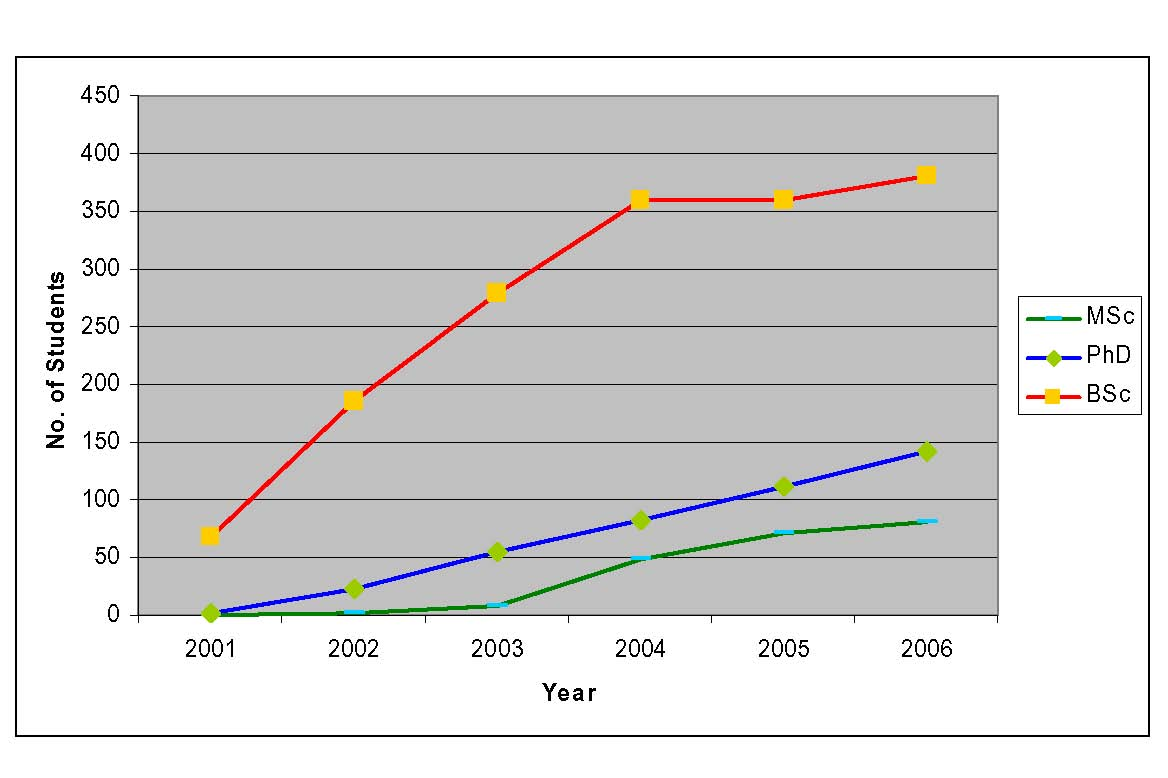
\includegraphics[width=\hsize]{Students.jpg}
   \end{center}
\caption{Temporal Development of Number of Students in the School of
Engineering and Science \label{fig:students}}
\end{figure}

\label{students}

\subsubsection{Publications}

During the founding period, the scientific output of the School,
measured in terms of the number of publications, has been growing
from initially 144 to 389 in 2006, after an intermediate decrease in
2004 which can be understood by having in mind that 2004 has been
the year during which the main research laboratories have been
planned and constructed (Fig.~\ref{fig:publications}). The last of
the laboratories (the EON laboratory) has been finished in 2005.

\begin{figure}[ht]
  \begin{center}
   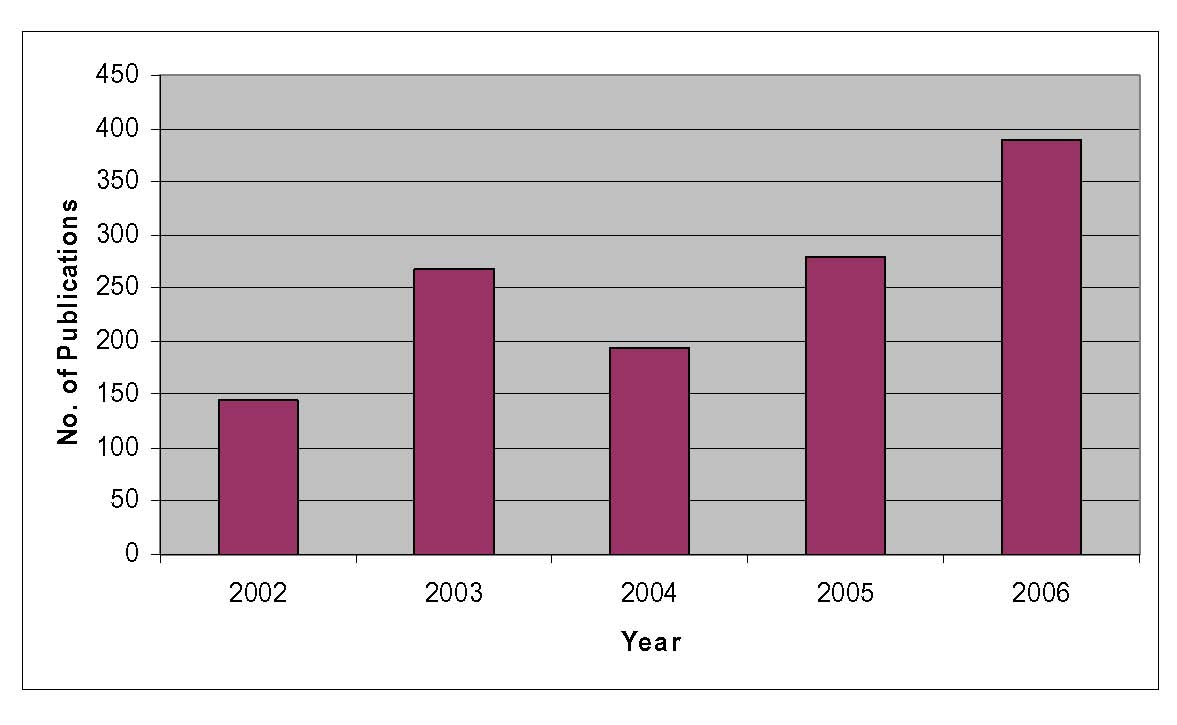
\includegraphics[width=\hsize]{Publications.jpg}
   \end{center}
 \caption{Number of Peer-reviewed Articles, Conference Proceedings, Articles in Encycl./Handbooks,
 Monographs/Books, Editor-ship, and Contribution in Ed. Volumes
 \label{fig:publications}}
\end{figure}


\subsubsection{Grants}
The development of third party funding is summarized in Figures
\ref{fig:grants1}, \ref{fig:grants2}. Revenues from Research grants
have reached a total of more than 4.000.000 EURO in 2006 which
implies an average revenue per professor of 82.000 EURO.

\begin{figure}[ht]
  \begin{center}
   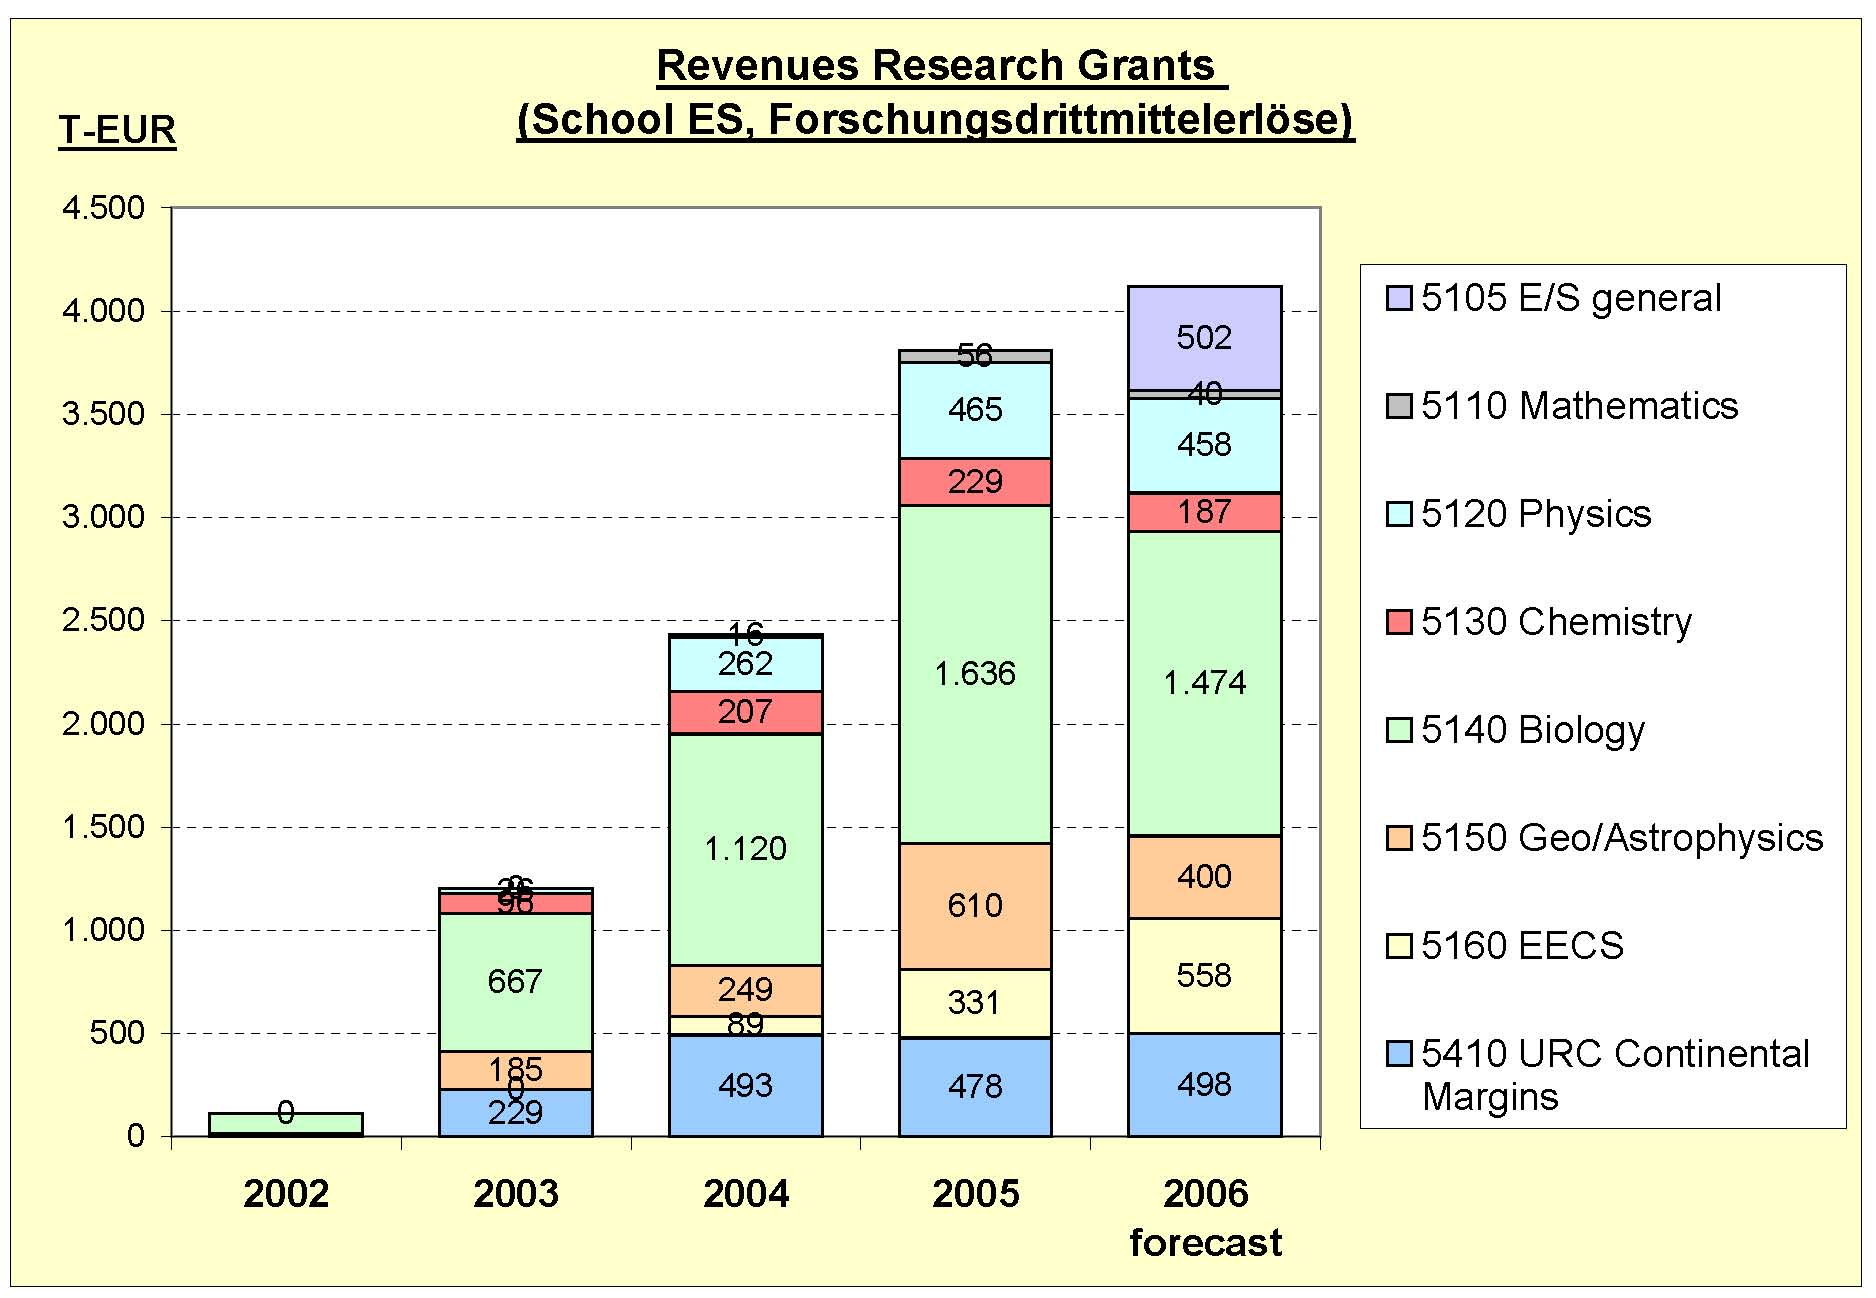
\includegraphics[width=\hsize]{SchoolESGrants-Charts1.jpg}

   \end{center}
 \caption{Research Grants  Revenue
 \label{fig:grants1}}
\end{figure}

\begin{figure}[ht]
  \begin{center}
   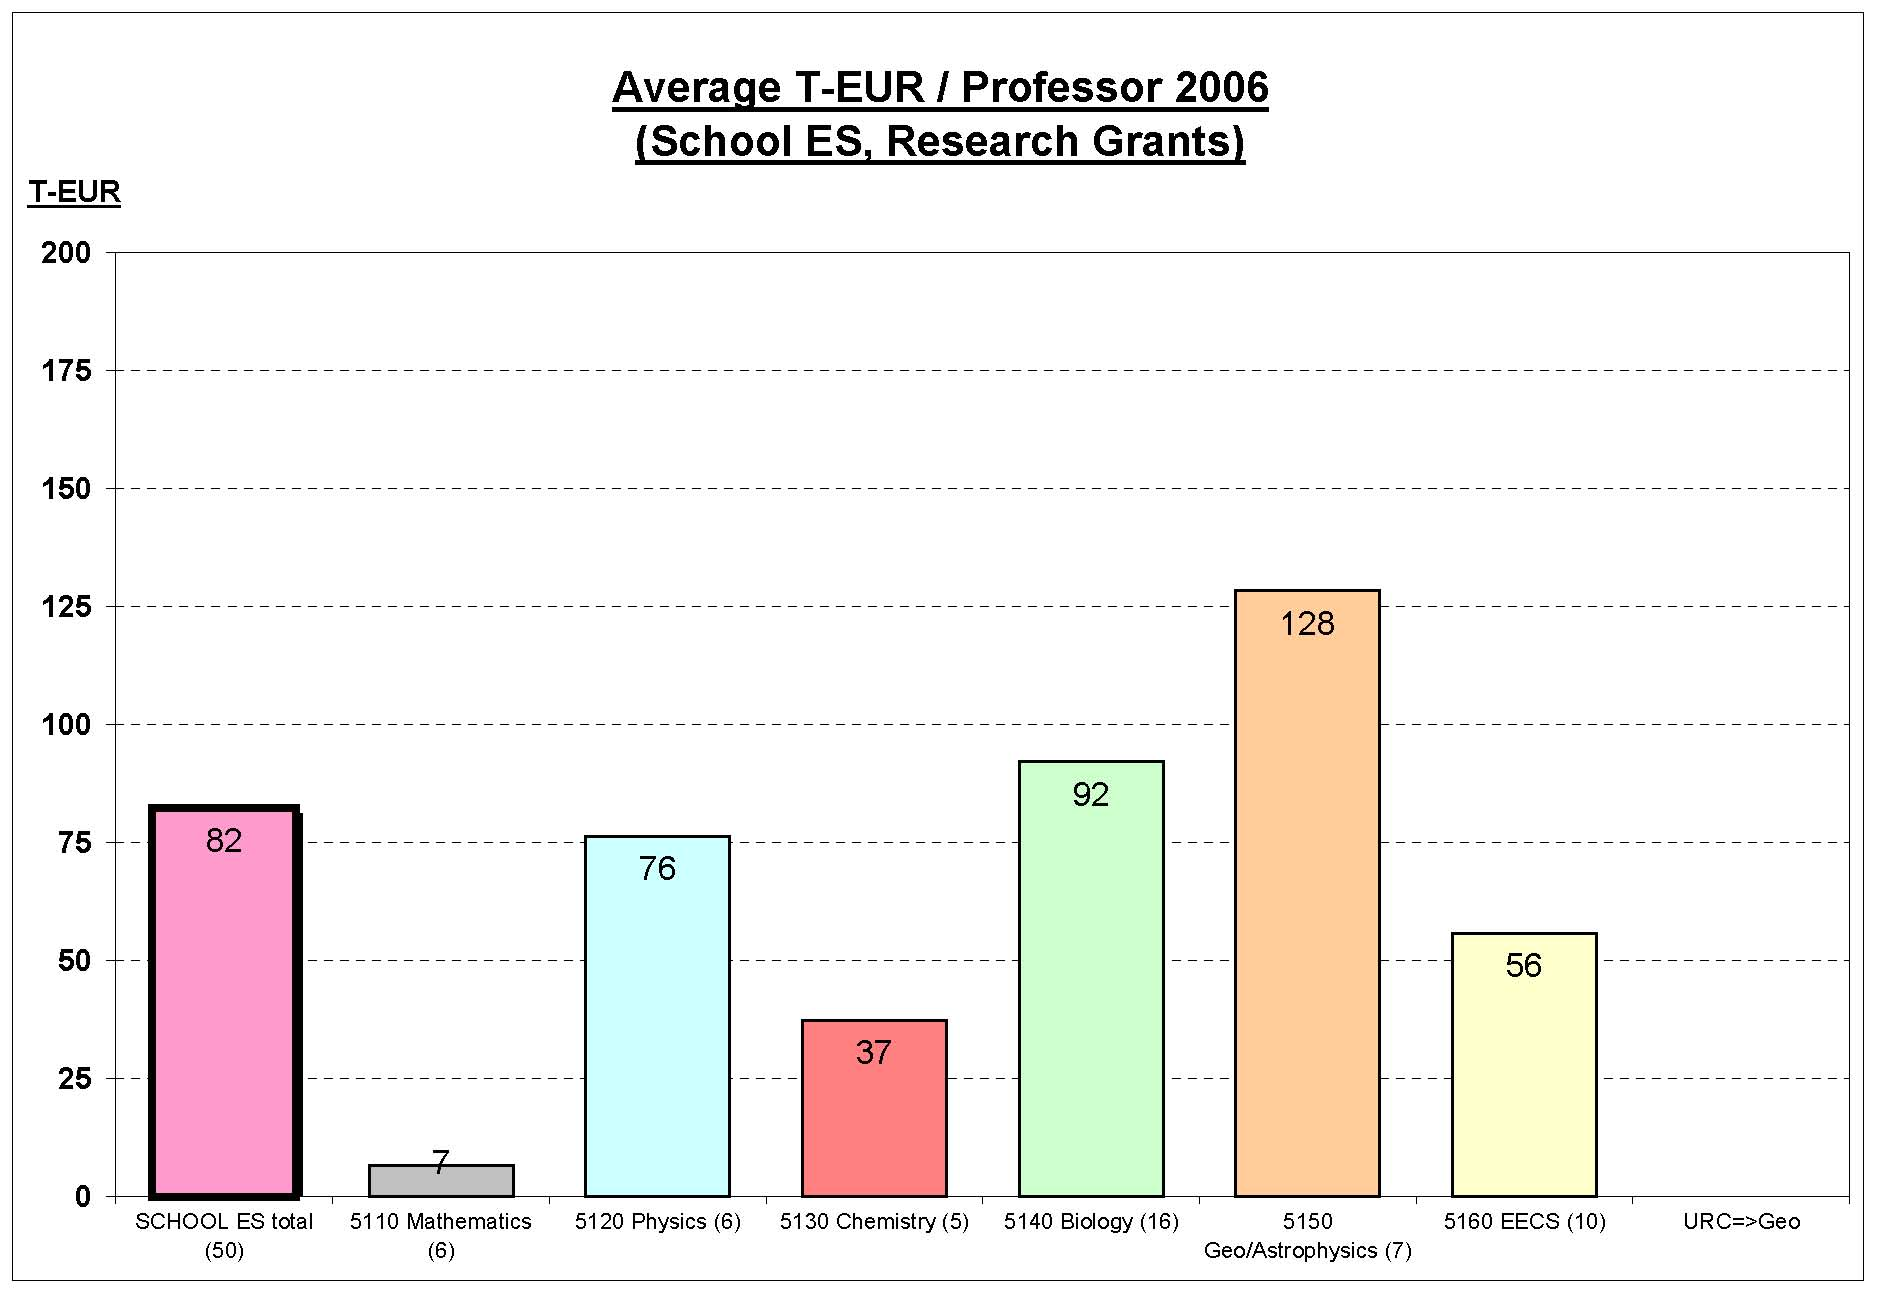
\includegraphics[width=\hsize]{SchoolESGrants-Charts2.jpg}
   \end{center}
 \caption{Research Grants Average T-EUR/Professor
 \label{fig:grants2}}
\end{figure}

\subsection{Personnel 2006} Presently, the school comprises in
total 64 professors out which 4 are adjunct professors, located at
the Alfred-Wegner-Institut in Bremerhaven and the Max-Planck-Insitut
f�r Marine Mikrobiologie in Bremen. Two distinguished professors and
6 university lecturers complete the faculty. In addition, 70
research associates, 5 research assistants, 26 technicians, 1
director and 7 assistants belong to the staff. In 2006, several new
faculty members have been hired.

\begin{myitemize}
 \item   Dr. Ulrich Kleinkath\"ofer, Associate Professor of
Theoretical Physics \item  Jon Wallace, PhD, Assistant Professor of
Electrical Engineering \item  Dr. Lars Linsen,  Associate Professor
of Computational Science and Computer Science \item   Dr. Bendick
Malehko, University Lecturer in Computer Science.
\end{myitemize}

In Mathematics, the visiting professors Prof. G. Litvinov and Prof.
Vladimir Tikhomirov, and Dr. Marc Comerford (research instructor)
left. They are replaced by \begin{myitemize} \item  Dr. Stefan Baier
(Visiting Lecturer for Mathematics) \item Kaivan Mallahi-Karai (PhD,
Visiting Lecturer for Mathematics) \item Dr. Alexei Belov (Visiting
Professor for Mathematics).
\end{myitemize}

The following members of the faculty have been promoted during 2006.
\begin{myitemize}
\item  Dr. Klaudia Brix from Associate to Full Professor
\item Dr. Albert Jeltsch from Associate to Full Professor
\item   Dr. Laurenz Thomsen from Associate to Full Professor
\item Marcus Br\"uggen Assistant to Associate
\item Claus C. Hilgetag, PhD from Assistant to Associate
\item Dr. Ulrich Schwaneberg from Assistant to Associate
\end{myitemize}

\null
Dr. Stefano Carpin, Assistant Professor of Computer Science,
has accepted an offer of an Assistant Professorship at University of
California, Merced, USA, starting on January 1, 2007.

\subsection{International Center for Transdisciplinary Science}
 The "International Center for Transdisciplinary Studies"
has been founded and started to operate. The center invites
internationally highly ranked scientists as fellows for periods of
several weeks, mostly during the summer break. The visiting
scientists are generally expected to participate in ongoing
scientific activities. In 2006, 46 scientists have been
participating, among them 39 from foreign countries:

\null Professor Dr. Roland Benz,   Universit\"at W\"urzburg, Germany
\\
Professor Dr.~Jan Bergstra,  University of Amsterdam, The Netherlands\\
Dr.~Andrey Bessonov, University of Sankt Petersburg, Russia\\
Dr.~S.M. Bezrukov,  National Institute of Health, Bethesda, USA\\
Dr. Georges Bouzerar,   Laboratoire Louis Nel, Grenoble, France\\
Dr. Henk Bruin  University of Surrey, United Kingdom\\
Professor Dr.~Mark Burgess,  University College Oslo, Norway\\
Professor Dr.~Val\'erie Cabuil,     Universit\'e Pierre et Marie
Curie, Paris, France\\
Dr.~Fabio Cavaliere, Universit\'a di Genova, Italy, Professor
Dr.~Shengbo Chen,      Institute of Geography and Natural
Resources, Beijing, China\\
Elizabeth Dan-Cohen,     University of California, Berkeley, USA\\
Professor Dr.~Gero Decher,      Institut Charles Sadron, Strasbourg,
France\\
Dr.~Martin Evans,        University of Edinburgh, United Kingdom\\
Dr.~Tom Fisher,      University of Cambridge, United Kingdom\\
Dr.~Claus F\"utterer,       Institut Curie, Paris, France\\
Professor Dr.~Mariano Grasselli,     Universidad Nacional de
Quilmes,
Argentina\\
Dr.~Giovanni Indiveri,       University of Lecce, Italy\\
Professor Dr.~Dieter J\"ager,      Emory University Atlanta, USA\\
Professor Dr.~Larry S. Liebovich,        Florida Atlantic
University,
USA\\
Professor Liviu Movileanu,      Syrakuse University, USA\\
Dr.~Sergei Nechaeev     CNRS Orsay, France\\
Professor Dr.~Catherine O'Neill,     Columbia University, USA\\
Dr.~Marieke Postma,     NIKHEF, Amsterdam, The Netherlands\\
Dr.~Enrico Ramirez-Ruiz,     Institute of Advanced Studies,
Princeton, USA\\
Professor Dr.~Helmut Ringsdorf,      Universit\"at Mainz, Germany\\
Dr.~Karin R\"omisch,       University of Cambridge, United Kingdom\\
Lucile Sassatelli,       ENSEA-ETIS, Cergy-Pontoise, France\\
Professor Dr.~J\"urgen Schnack,        Universit\"at Osnabr\"uck,
Germany\\
Professor Dr.~Gerhard Schwarz,       Biozentrum Basel, Switzerland\\
Professor Dr.~Vera Serganova,        University of California,
Berkeley, USA\\
Professor Dr.~Nobuo Shimamoto,      National Institute of Genetics,
Mishima, Japan\\
Professor Dr.~Canan Tari,        Izmir Institute of Technology,
Turkey\\
Professor Dr.~Alexander Tikhomirov,  Yaroslavl State Pedagogical
University, Russia\\
Dr.~Andrew Travers,      Medical Research Council, Cambridge, United
Kingdom\\
Dr.~Martin Weigt,        ISI Foundation, Torino, Italy\\
Professor Dr.~James Whisstock,      Monash University, Victoria,
Australia\\
Dr.~Wojtek Zakrzewski,   University of Durham, United Kingdom\\
Dr.~Michael Zaks,    Humboldt-Universit\"at Berlin, Germany\\
Professor Dr.~Gregg Zuckerman,   Yale University, USA.

\subsection{Workshops and Summer Schools 2006}

During the year, several international research workshops have been
organized on the campus by members of the faculty.

\begin{myitemize}
\item
From October 19-22, 2006 the International Workshop on Astrobiology
took place at IUB, organized by Professor Michael Bau.  Focus of the
workshop were Banded Iron Formations (BIFs), that developed between
two and four billion years ago in the precambrian era.  The workshop
aimed at providing an overview on current ideas on the formation and
preservation of Precambrian BIF, on the use of BIF as proxies for
Precambrian seawater, on differences between Early Precambrian BIF
and younger ironstones and hydrogenetic Fe(-Mn) precipitates, and on
experimental set-ups to simulate BIF-related processes in Early
Precambrian environments.

\item
A workshop for young scientists is offered biannually by the DFG
Schwerpunktprogramm SPP1170 (priority program) ''Directed Evolution
to Optimize and Understand Molecular Biocatalysts''. This year's
workshop  took place from July 30 until August 1 on the IUB campus,
organized by Professor Ulrich Schwaneberg. 70 scientists from the 17
DFG institutions participate in the program. They presented and
discussed the research and its influence on applications with
representatives from companies.


\item
From July 28 until August 5, a Summer School for students and
postdocs  took place. Focus of the more than 50 lectures and
workshops has been on recent research perspectives in biosensing and
its application. 70 participants from 14 Nations met on IUB campus.
This summer school  covered applications of membrane channels in
molecular biology and biotechnology. In addition, it informed on the
underlying physics and will present recent advances in microfluidics
and nanoelectronics. The fourth IUB Summer School has been organized
by Dr. Mathias Winterhalter, Professor of Biophysics at IUB. The
Summer School offered students and postdocs the opportunity to
advance their understanding of biosensing, present their research
and build networks.


\item In June 2006, the 10th International RoboCup has been organized
in Bremen. More than 400 teams and 2500 participants from 36
countries participated and competed in three main categories: the
robot soccer competition, the robot rescue competition (coordinated
by Prof. A. Birk), and the RoboCupJunior for educational purposes.
On June 18, the finals of the Robot Rescue League took place in the
Congress Center Bremen. IUB teams participated in both competitions
the ''Rescue Robot League�� and the ''Virtual Robot Competition��.
The team led by Andreas Birk, Professor of Electrical Engineering
and Computer Science, reached the finals of the Robot League and won
the Innovation Award, a student team led by Stefano Carpin,
Professor of Computer Science came in second place in the Virtual
Robot Competition.

\item
From the 16th to 20th of January, IUB  hosted the international
"HERMES Graduate Training and Job Fair". More than 30 Master's and
PhD students working at HERMES partner institutions all over Europe
participated. The fair offered students and Postdocs the opportunity
to advance their understanding in aspects of marine science outside
their own fields and to present and discuss their own research (Jan
10, 2006). The HERMES (Hotspot Ecosystem Research on the Margins of
European Seas) Program, funded by the European Commission, was begun
to gain better understanding of life in depths of between 200 and
2000 meters and deeper.

\end{myitemize}


\subsection{Research Highlights}

Researchers of the School of Engineering and Science have been
contributing towards the international scientific progress with
several important discoveries that have been published in the most
prestigious international journals.

\begin{myitemize}
\item
Albert Jeltsch, IUB Professor of Biochemistry, and his co-workers
from IUB, the Institute of Biochemistry of the University of
Giessen, and the Medical Research Council of Cambridge University
(UK) for the first time successfully used genetically engineered
proteins to deactivate Herpes viruses in human cell lines. The study
is published in the November 2006 issue of Nucleic Acids Research

\item
Stefan Tautz, IUB Professor of Physics, and his group for the first
time managed to detect a much larger delocalization of electrons in
an organic monolayer semiconductor deposited on a metallic substrate
than ever detected in an insulated organic semiconductor. The
results, which were published in Nature 444, p. 350 - 353, on
November 16, 2006, allow insights into basic mechanisms of electron
transport within organic materials and their interfaces with
metallic surfaces. Moreover, the results may be of relevance for the
development of new hybrid materials with interesting new electronic
properties regarding future application.



\item
On the 68th cruise of the German research vessel METEOR an
international team of scientists under the lead of Andrea
Koschinsky, Professor of Geosciences at IUB, registered 407
$^{\circ}$ C at a hydrothermal vent as the highest temperature on
record measured at the ocean bottom (May 22, 2006).  Using a special
temperature sensor operated by a deep-sea robot the scientists
registered the record temperature in 3000m water depth at a
so-called ''black smoker'', a hydrothermal deep-sea vent with a
characteristic particle plume in the discharge water. Moreover, the
boiling fluids emitted by the vent were filmed. The super-hot vent
was discovered at 5 $^{\circ}$ S at the Mid-Atlantic Ridge, where
the African and the South American continental plates drift apart 4
cm per year, causing increased volcanic activity. Normally the
temperature of the circulating seawater cooling the volcanoes
emerging in this area does not exceed a maximum of about 350
$^{\circ}$ C when welling out of the sea floor. Maximum deep-sea
water temperatures up to 402 $^{\circ}$C so far have only been
observed in the Pacific.




\item
Stephan Rosswog, Professor of Astrophysics at IUB, and Daniel Price,
Postdoc at the University of Exeter, for the first time were able to
demonstrate in supercomputer simulation of a neutron star merger
that a collision of these super dense cosmic objects create magnetic
fields a quadrillion (10$^{15}$) times stronger than the magnetic
field of the earth. The simulation results are published in the
current online express issue of Science ("Producing ultra-strong
magnetic fields in magnetized neutron star mergers", 30 MARCH 2006).

\item
Claus Hilgetag, Professor of Neuroscience at IUB, and his colleague
Helen Barbas, Professor of Health Sciences at Boston University,
found new answers to one of the oldest questions in neuroscience:
How do the characteristic folds of the primate brain cortex form?
The results of an extensive analysis of neuroanatomic data are
published as the cover story in the latest issue of PLoS
Computational Biology ("Role of Mechanical Factors in the Morphology
of the Primate Cerebral Cortex", Volume 2, Issue 3, MARCH 2006,
www.ploscompbiol.org).  By analyzing quantitative data collected in
the lab of Helen Barbas over a period of two decades, Claus Hilgetag
for the first time was able to provide empirical evidence for the
hypothesis that the characteristic folds of the primate brain are
mainly formed by mechanical forces of fiber tension.


\end{myitemize}


\subsection{Noteworthy}
\begin{myitemize}
\item
On November 15, 2006, the association ''Unifreunde e. V.�� awarded
the Ernst A. C. Lange Prize for the joint research project ''New
display technology for mobile applications�� of IUB and University
of Bremen. The award, which is endowed with 5000 euros prize money,
acknowledges innovative co-operational research between scientists
of the two Bremen universities in the fields of Mathematics, Natural
and Technical Sciences. The two laureates 2006 are the two Bremen
scientists Dietmar Knipp, Professor of Electrical Engineering at
IUB, and Wolfgang Benecke, Professor of Physics, Electronics and
Information Technology at University of Bremen. The aim of their
joint research project is the development of a new type of
projection display for mobile application such as laptop computers,
mobile phones, and digital cameras.


\item Researchers from all over Germany were taking part in the Science
Festival "Highlights of Physics" from 6-10 November 2006 in Bremen.
Under the motto of "WaveWorlds" scientists gave an introduction into
wave phenomena in water, light and sound through series of talks,
live experiments and science shows.  IUB was involved in the
organization and preparation of this event. Faculty and staff
contributed in particular to the big opening show, the exhibition,
and the physics competition for pupils.

\item
In October the research network International Research Consortium on
Continental Margins (IRCCM) under IUB's lead started a new research
project on biomonitoring of cold water coral reefs in the vicinity
of oil exploration sites. The aim of the 1.2 million euro project
financed by the Norwegian company Statoil is to develop new
monitoring and ecosystem modelling approaches for risk assessment in
the off-shore industry.  Research site is the Tisler cold water
coral reef in the Skagerrak, which was placed under environmental
protection by the Norwegian government in 2003. As part of the EU
HERMES project (Hotspot Ecosystem Research on the Margins of
European Seas) it is managed by HERMES partner Tj\"arn\"o Marine
Biological Laboratory (TMBL) and will host IUB's second deep-sea
online observatory.


\item
On April 23, 2006, IUB's RoboCup team managed another international
tournament victory at the US Open Robot Rescue League in Atlanta,
prevailing against the other competing institutions only two weeks
after their success at the Dutch Open in Eindhoven (Apr 25,2006).
The ten contesting teams in Atlanta included such renowned
institutions as the Georgia Institute of Technology and Carnegie
Mellon University, which demonstrated with their impressive
investments into their teams the importance of research on search
and rescue robots in the US. Georgia Tech had two teams within the
competition, one of them using the best mobile research platform
that is currently available on the market. A team from Carnegie
Mellon University had even six robots running including a high-end
commercial platform for search and rescue missions.

\item
Informatics Year is being organised in conjunction with the Science
in Dialogue initiative and the Gesellschaft f�r Informatik (GI) as
well as with numerous partners in the fields of science, industry
and culture. The idea behind this Science Year was to familiarise a
broader public with the contents, processes and practical
applications of science and to do so in an informative, exciting and
entertaining way. IUB was involved in exhibitions, the Symposium on
Artificial Intelligence and various other activities.

\end{myitemize}
\ \ \\
\ \ \\

Bremen, January 2007


\begin{figure}[ht]
     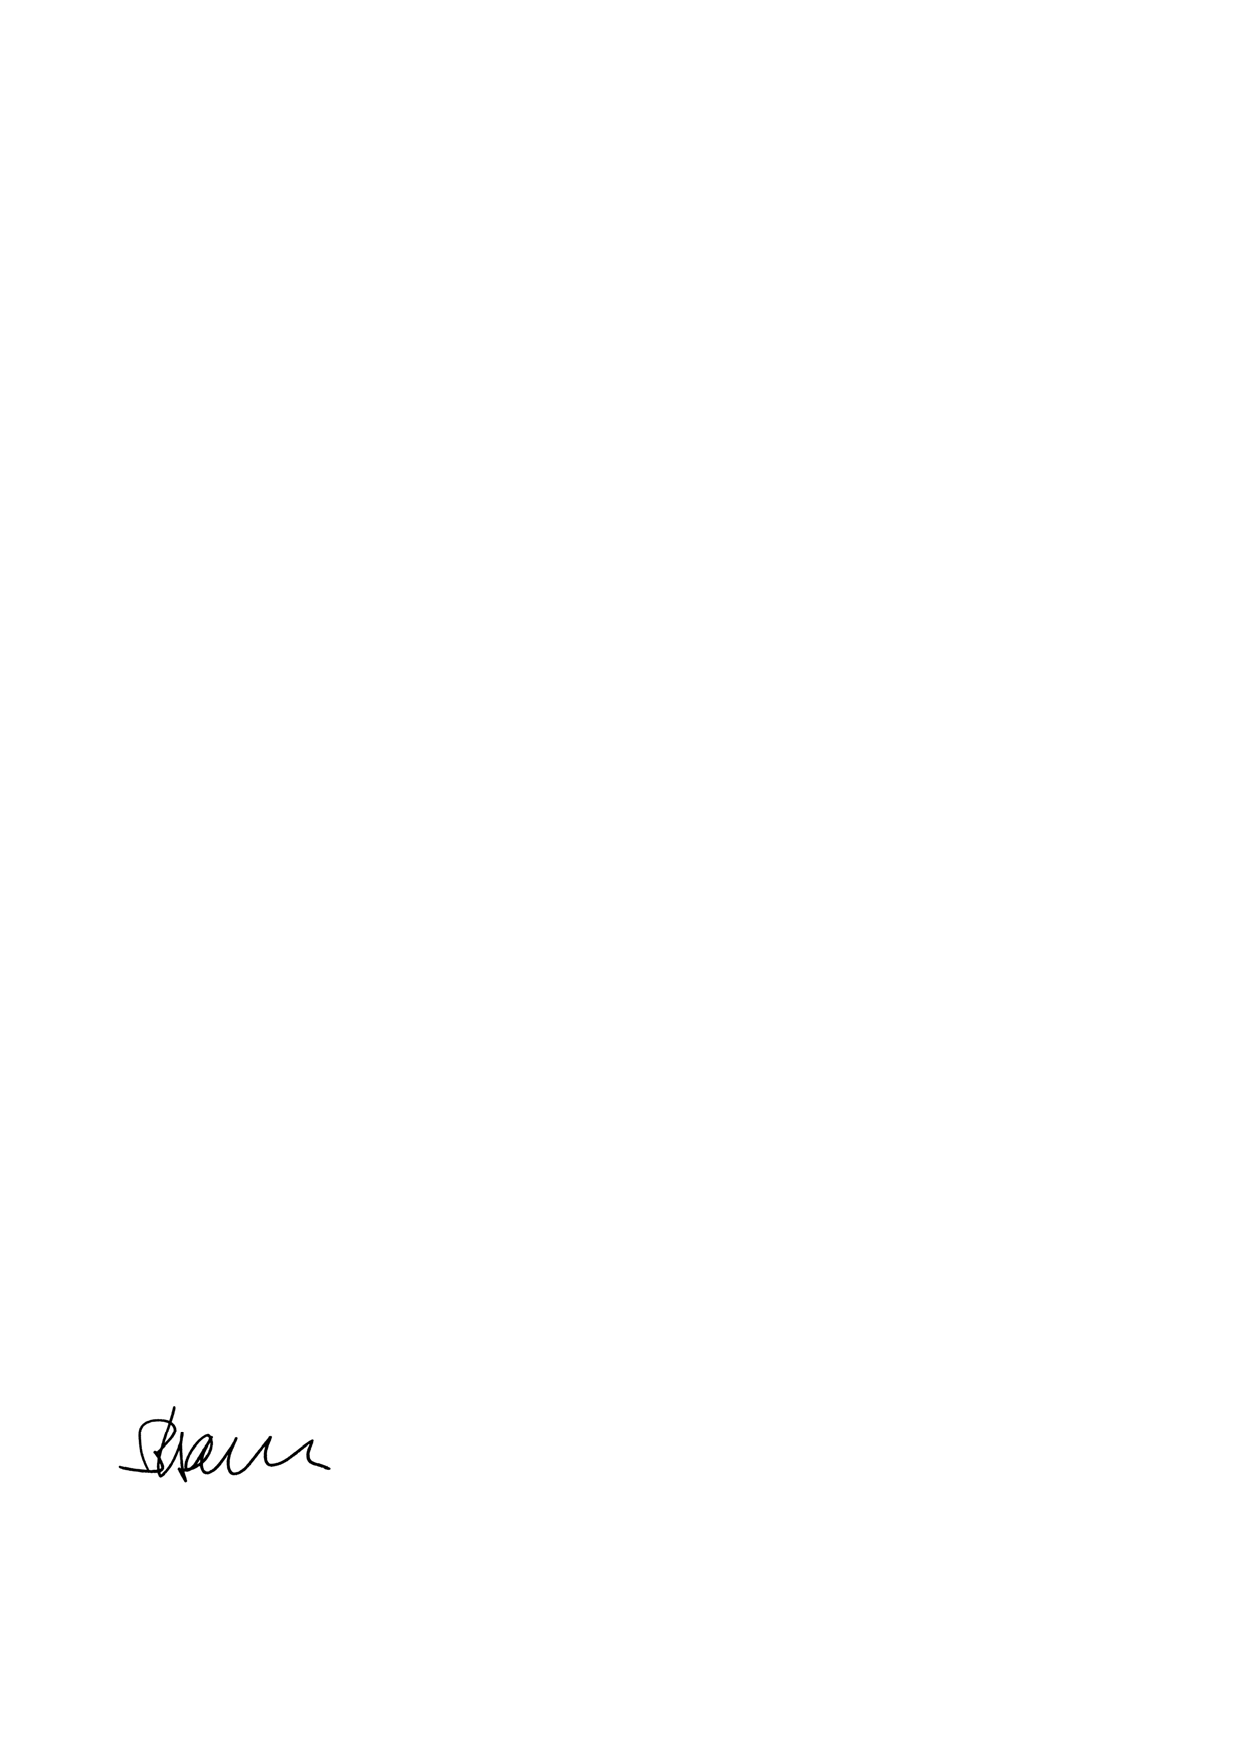
\includegraphics[width=4cm]{DeanSig}
 \end{figure}



Bernhard Kramer
 \cleardoublepage
%\bibliographyunit[\subsection]
\shorttitle{Information and Communication Technologies}
\section{Information and Communication Technologies}

The increasing impact of information and communication technology dominates our everyday
life, our society, and the environment.  Examples comprise the World-Wide-Web, the
ubiquitous use of computers, cellular multimedia and wireless communications, robots in
factories as well as in offices and homes, and sophisticated computer models used to
predict the evolution of complex systems such as the global climate.

The enormous level of integration in micro-electronics has enabled unprecedented progress
in many sectors -- and even more importantly, it has created many new profitable
technologies and services based on them. The 21st century will witness technologies that
enable machines to do things that have been so far restricted to humans: machines will be
able to sense, act, speak, listen, decide and sometimes understand. Our T-shirts may have
their own Internet addresses and wirelessly tell the laundry machine about proper
treatment. We will see cars that negotiate with each other in order to maximize traffic
flow while reducing pollution using sophisticated energy management systems. Manufacturing
technologies will improve using a combination of detectors and software to control
processes. Robots are also more and more used in domains where some autonomy and
intelligence is necessary. They work under conditions where it is unpleasant or even risky
for humans like in abandoned mines or at disaster sites and where they have to deal with
situations unforeseen by their designers and programmers. The hallmark of such smart
systems is their integration of technologies from analogue devices and sensors,
communication systems and networks, internet services, artificial intelligence, machine
learning, robotics, and many more.

The School of Engineering and Science actively contributes to this
rapidly growing, boldly interdisciplinary endeavor, focusing on the
areas described in the following.
%
%{\em{Mathematical and Symbolic Modeling}\\
%  \item Reasoning and Semantics
%  \item Simulation and Control of Complex Systems
%  \item Machine Learning
%  \end{itemize}
%\item {\em{Communication Networks and Systems}}, in particular:
%  \begin{itemize}
%  \item Wireless and Cellular Communications
%  \item Digital Transmission Methods and Coding
%  \item Networks and Protocols
%  \item Harmonic Analysis applied to communications engineering
%  \end{itemize}
%\item {\em{Robotics and Embedded Systems}}, in particular:
%  \begin{itemize}
%  \item Robotics
%  \item Applied Algorithms
%  \end{itemize}
%\item {\em{Knowledge and Information Management Systems}}, in
%  particular:
%  \begin{itemize}
%  \item Raster Data Services
%  \item Knowledge Management Systems
%  \item Distributed Systems
%  \item Hierarchical Data Representation
%  \end{itemize}
%\item {\em{Microelectronic Devices and Technologies}}, in particular:
%  \begin{itemize}
%  \item Electronic Devices and Nano Photonics
%  \item Microelectronics
%  \end{itemize}
%\item {\em{Digital Signal Processing}}, in particular:
%  \begin{itemize}
%  \item Signal Processing in Communications
%  \item Nonlinear Signal Processing and Control
%  \end{itemize}
%\end{enumerate}

%%% Local Variables:
%%% mode: latex
%%% TeX-master: "report"
%%% End:

\shorttitle{Communication Networks and Systems}
\subsection{Communication Networks and Systems}

The basic desire of modern society to be able to access and
distribute ``any'' information at ``anytime'' and ``anywhere'' is
the driving force for the rapid development of communication
networks and systems. The implications of these goals are manifold
and require truly interdisciplinary research efforts. A typical, but
clearly not complete, list of involved high level research fields
includes

\begin{myitemize}
\item Wireless Network Engineering and System Design
\item Network Interoperability
\item System capacity management and optimization
\item Information transmission
\item Network protocols 
\item Information security.
\end{myitemize}

All these research areas are strongly inter-related and the strength
of a research cluster in ``communication networks and systems''
resides in the close cooperation of the respected research groups
involved. The particular `flat hierarchy' at IUB (no departments and
chairs) fosters such cooperations.

%%% Local Variables:
%%% mode: stex
%%% TeX-master: "report"
%%% End:

\begin{bibunit}[hplain]
  
\subsubsection{Cellular and Wireless Communications}
\label{Haas1} \index{Haas, Harald}

\paragraph{Research Team}
Harald Haas (Professor), Rami Abu-Alhiga (PhD Student), Zubin
Bharucha (PhD Student), Hany Elgala (PhD Student), Ellina Foutekova
(PhD Student), Birendra Ghimire (PhD Student), Dennis Kolyuzhnov
(PhD Student),  Raed Youself Mesleh (PhD Student), Abdurazak Mudesir
(PhD Student), Hrishikesh Venkataraman (PhD Student), Sinan
Sinanovic (Research Associate), Peter Omiyi (Postdoc), Mostafa
Afgani (Research Engineer), Sudharasan Ganesan (Graduate Student)\\

Research in Cellular and Wireless Communications is geared towards
new technologies. Particular focus is  on the development and the
interaction of key air-interface building blocks \newpage

\begin{myitemize}
\item multicarrier transmission (in particular OFDM (Orthogonal Frequency Division
Multiplexing)
\item duplexing techniques (in particular time division duplexing
(TDD))
\item multiple-input multiple-output (MIMO) techniques
\item wireless ad hoc systems
\item medium access control (MAC) algorithms
\item multiple access and scheduling techniques
\item dynamic channel assignment (DCA) algorithms
\item mobile positioning
\item visible light communication.
\end{myitemize}

\myparagraph{Highlights} \emph{Spatial Modulation.} Spatial
modulation (SM) is a new and patented multiple antenna transmission
approach for wireless systems that increases the spectral efficiency
(number of bits transmitted per Hz bandwidth) by utilizing the
transmit antenna number as an implicit source of information. A
block of information bits is mapped to an information symbol and a
transmit antenna number. As a consequence, at any given time instant
only a single antenna of the antenna array is transmitting signal
power. The actual block of information bits determines which antenna
is active at a particular time instant. As a result, inter-channel
interference (ICI) at the receiver input and the need to synchronize
the transmit antennas are completely avoided. Simple receiver
algorithms such as maximum receive ratio combining (MRRC) can be
used to retrieve the information bits. The performance and the
receiver complexity of SM and V-BLAST (Vertical-Bell Labs Layered
Space-Time) algorithm in flat fading channels are compared. V-BLAST
applies zero forcing detection based optimum ordering, nulling and
successive interference cancellation. The basic principle of SM is
depicted in Fig.~\ref{smexmpl}, and results of the comparison with
state-of-the-art V-BLAST are shown in Fig.~\ref{fig55}.
\begin{figure}[!htb]\centering
  \centerline{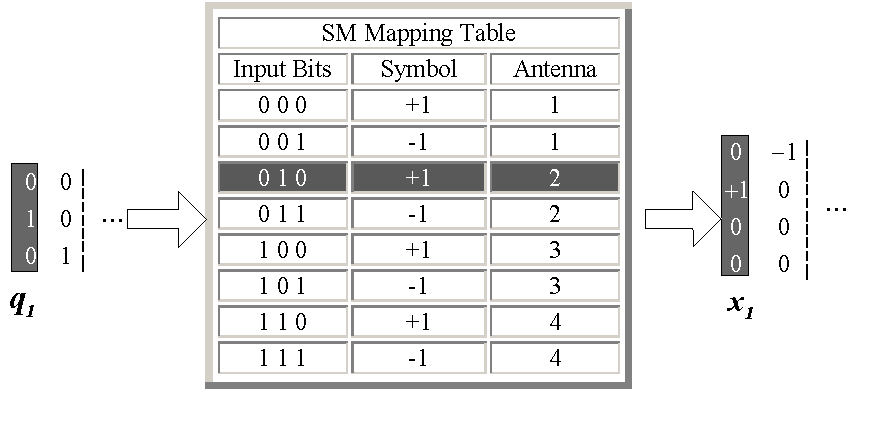
\includegraphics[width=8cm]{haas_1.pdf}}
  \caption{3bits/symbol spatial modulation mapping table using binary phase shift keying (BPSK)
    and four transmit antennas} \label{smexmpl}
\end{figure}
\begin{figure}[!!htp]\centering
  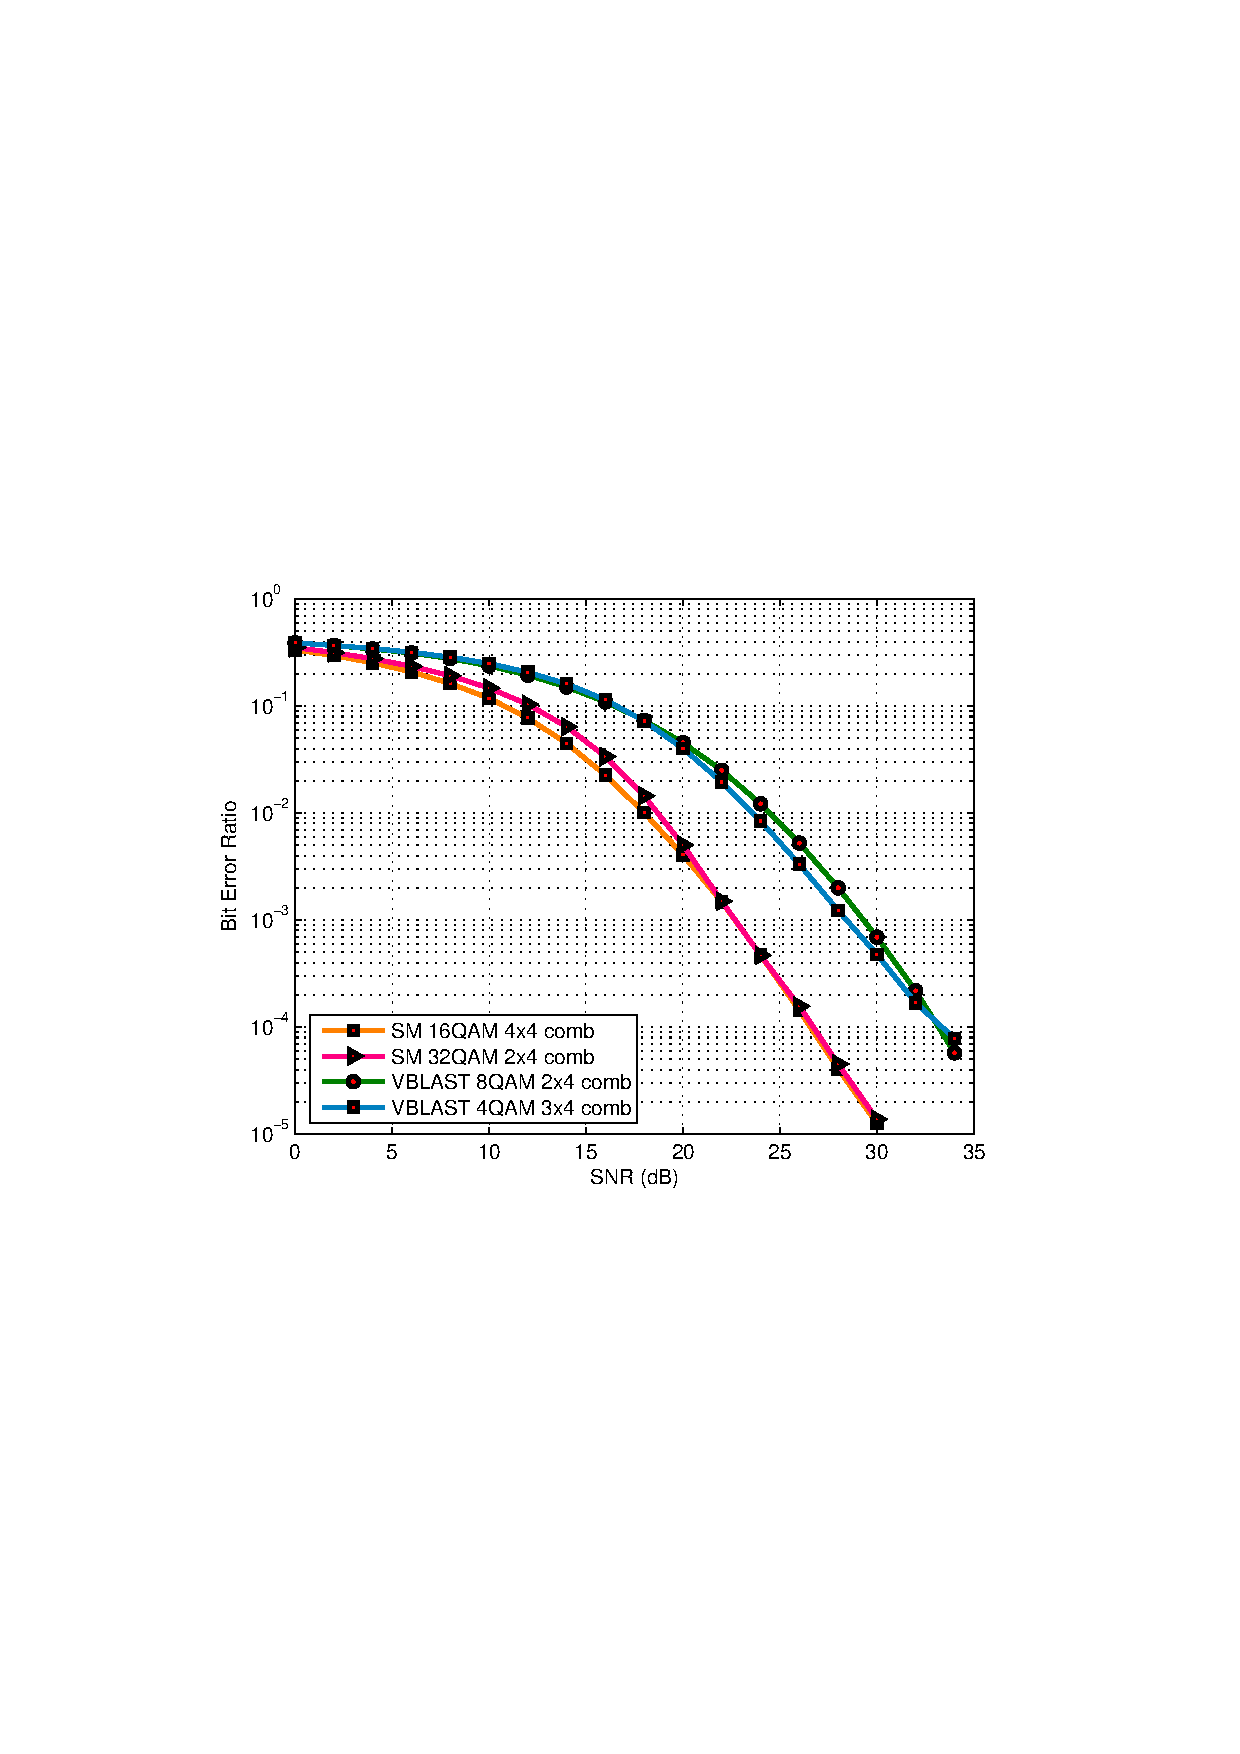
\includegraphics[width=8cm]{haas_2.pdf}\\
  \caption{Bit error performance as a function of signal-to-noise ratio (SNR) for state-of-the-art V-BLAST and novel SM.}
  \label{fig55}
\end{figure}
From the results it can be found that the performance gains are
significant. In both schemes the same number of bit per unit
bandwidth are transmitted (for fair comparison), but with SM the bit
error performance is reduced considerably. For example, at an SNR of
20dB a 10-fold reduction in the BER is observed.

\emph{Dynamic Resource Allocation.} In this work a fully
decentralized interference avoidance algorithm to manage
interference in an \emph{ad hoc} wireless network, applicable to
wireless sensor networks, is developed and analyzed. Fig.~\ref{dca}
depicts a randomly chosen distribution of transmitting (Tx) and
receiving (Rx) nodes. The new algorithm, called \emph{busy tone
interference tolerance signaling}, is of low complexity and is very
easy to implement. It is based on different functions to set the
busy tone signal power dependent on the level of tolerable
interference, and their performance is compared with a special case
of a fixed power system which provides maximum capacity assuming
equal transmit powers. Results show that an appropriately chosen
function for setting the busy-tone can lead to gains in capacity
using very little power. This power efficiency advantage is quite
significant, implying that battery life of units can be extended
while providing a similar capacity than a fixed power system.
\begin{figure}[!!htp]
 \centering
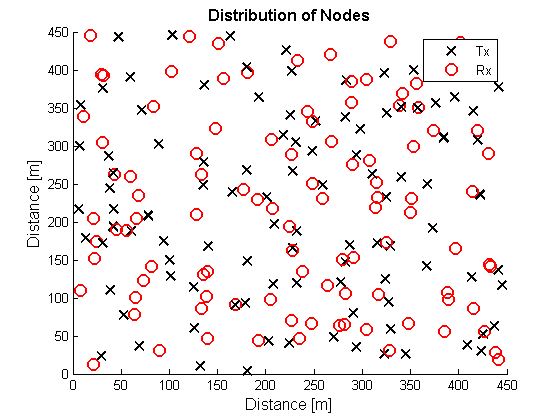
\includegraphics[width=8cm]{haas_3.png}\\
\caption{Random distribution of nodes in an \emph{ad hoc} wireless network}
\label{dca}
\end{figure}

%\null Harald Haas is also involved in ``Signal Processing''
%(Section~\ref{Haas1}).

%\newpage
\paragraph{Organization}
% list the (research) events you have organized, if any,
\begin{enumerate}
    \item Member of Technical Program Committee of and session chair
          at \emph{IEEE International Conference on Personal, Indoor \& Mobile Radio Communications} -- PIMRC 2006
    \item Member of Technical Program Committee of \emph{International IEEE Conference on Vehicular Technology} -- VTC 2006
\end{enumerate}

\paragraph{Collaborations}
\begin{enumerate}
\item {\sl The University of Edinburgh, UK}\\
  Prof. S. McLaughlin\\
  Joint project with industrial partner on \emph{Hybrid Cellular and Multihop Wireless
    Networks}
\end{enumerate}

\newpage
\paragraph{Grants}
% list the running grants in 2005, if none have been received, please delete this
% subsection.
\begin{enumerate}
    \item Funded by industry partner,
      \emph{Cellular TDD-OFDM (Time division duplex - orthogonal frequency
          division multiplexing)},  June 2004 - July 2005


    \item Funding by industry partner and University of Edinburgh, \emph{Hybrid Cellular and Multihop Wireless
    Networks},  July 2005 - July 2006

    \item Funded by industry partner, \emph{Link Adaptation and Scheduling in Cellular
    Systems},  March 2005 - February 2008

    \item Funded by Bremen T.I.M.E program funded by BIS
    Bremerhaven, \emph{Mobile Positioning (MPos)} in collaboration with MobilTec GmbH and supported by
     T-Mobile,  June 2006 - September 2009

    \item Funded by DFG Schwerpunktprogram TakeOFDM, \emph{DCA Algorithms and MAC Protocols for COFDM Based Cellular and
     Ad hoc Systems Using Carrier Sensing Time Division Multiple Access
     (CSTDMA)},  October 2004 - September 2006

\end{enumerate}

\paragraph{Patents}
% list the grants you have received in 2005, if none have been received, please delete this
% subsection.
\begin{enumerate}
\item Four new patent applications submitted
\item Three previously submitted patents got granted in 2006
\end{enumerate}

\paragraph{Awards, Prizes}
\begin{enumerate}
\item Nominated for the Chinese 111 Program -- Guest Academic Talents Programme for the Development of University Disciplines in China
\item Invited Talk at the University of Mondragon (Spain)
%    \item Honorary Fellowship of Edinburgh University
%    \item Invited to Institute for Digital Communications (IDCOM) at the University of
%          Edinburgh on \emph{Vodafone Fellowship on Communications}
    %\item Invited speaker at \emph{International Next Generation Wireless Network Workshop},
     %     Edinburgh/Scotland
\end{enumerate}

%\paragraph{Publications}
% list the publications of 2005 (also accepted and in press), if none have been received, please delete this
% subsection. Enter the publications into the SES publications database at
% http://kwarc.eecs.iu-bremen.de/ses-pubs/index.php and only reference them here.

 
\nocite{ah06_vis_light}
\nocite{bh06_ped_dead_reck}
\nocite{hnona06_iamac}
\nocite{vh06_thru_cap}
\nocite{cvh06_freq_syn}
\nocite{feh06_semi_analytic}
\nocite{fagvh06_sch_CDMA}
\nocite{jhm06_adhoc_tdd_underlay}
\nocite{oha06_tsalloc_insotdd}
\nocite{mhay06_spatialmod}
\nocite{asilomar06}
\nocite{chinacom06}
\nocite{tdd_book}
\nocite{oha07}
 

 
  \putbib[combined]
\end{bibunit}
\begin{bibunit}[hplain]
  \subsubsection{Digital Transmission Methods and Coding}
\label{ict:cns:henkel} \index{Henkel, Werner}

\paragraph{Research Team}
Werner Henkel (Professor), Fangning Hu (PhD Student), Neele von Deetzen (PhD
Student), Khaled Shawky Hassan (PhD Student), Apirath Limmanee (PhD Student)\\

We currently concentrate on iterative decoding and unequal error protection in
coding and physical transport. In iterative decoding, we study the convergence
behavior and properties of analog Turbo-like codes and the possible design of
Turbo and LDPC codes for unequal error protection (UEP). In the design of UEP
codes, we especially cooperate with ENSEA, France, and Lule\aa\ University,
Sweden. UEP is also the goal in our multicarrier research, where we design
bit-allocation algorithms that allow for easy realization of different
protection classes in an arbitrary way. UEP will be a must for current and
especially future triple-play data services to different devices at varying
channel qualities.

The analog codes have a strong relation to signal processing. Regarding
practical applications of such codes, we especially look into the correction
of impulse-noise and clipping effects. There, the most important task is to
determine statistical properties that allow for easy erasure marking, which
would support further decoding steps, analog and digital.

We further started a project on data transmission using ultrasound signals. We
currently design lab experiments to deliver data for later modeling of the
channel and disturbances.

%%% give a very short (150 words description of your research area)
%% Hint: this can be copied from the research areas document (../masterplan/research-areas)

\paragraph{Highlights}

The design of UEP Turbo codes by a pruning approach led us to a structure that
we named hybrid concatenation, a combination of outer parallel and inner
serial concatenation. The study of the decoding convergence with so-called EXIT
charts yielded the result that the area between the curves describing the
outer iterations depend on the number of inner iterations. This allows for
minimizing the decoding complexity by a scheduling with varying number of
iterations in the different decoding steps (see Fig.~\ref{fig:henkel_1}). The
pruning concept was also the starting point for our design of UEP LDPC codes
with an irregular check-node profile (pat. pending).

\begin{figure}[ht]
  \centering
  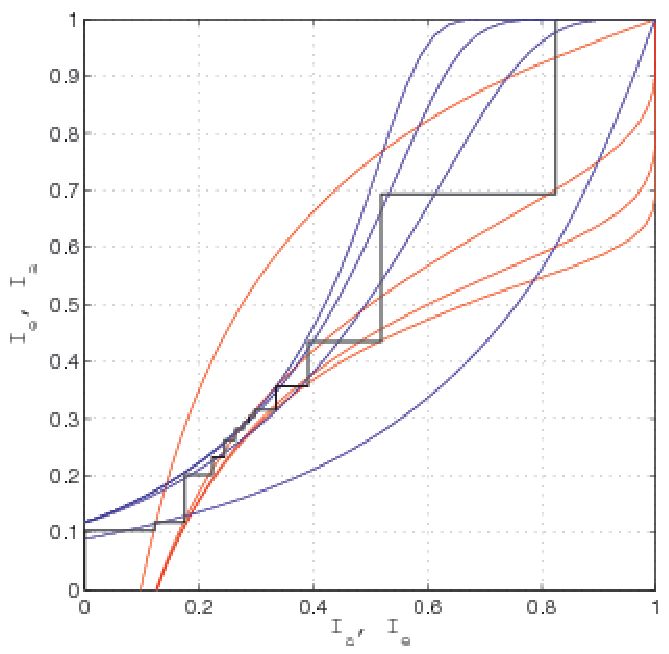
\includegraphics[width=7cm]{henkel_1}
 \caption{Convergence scheduling for hybrid concatenation}
%  \caption{Convergence scheduling for hybrid concatenation}
  \label{fig:henkel_1}
\end{figure}

In analog coding, we further improved the presentation of our proof that
Turbo-like decoding leads to a least-squares solution. We can now exactly
forecast the convergence limits for the stepsize and can also
modify it for every iteration to allow for very fast
convergence. For impulse-noise detection, we currently investigate new
statistical properties, e.g., the slope distribution, and correlation
approaches. This study will also close a gap in impulse-noise modeling
regarding the autocorrelation function of impulse noise.

By designing a new bit-allocation algorithm (pat. pending), following the
principles of an existing one by Chow, Cioffi, and Bingham, we can obtain UEP
properties in a very elegant way. It allows for an arbitrary number of
error-protection classes with arbitrary margins between them and an arbitrary
number of bits per class. Figure~\ref{fig:henkel_2} shows a resulting bit and
power allocation according to the channel SNRs, assuming three error protection
classes with a 3 dB separation.


\begin{figure}[ht]
  \centering
  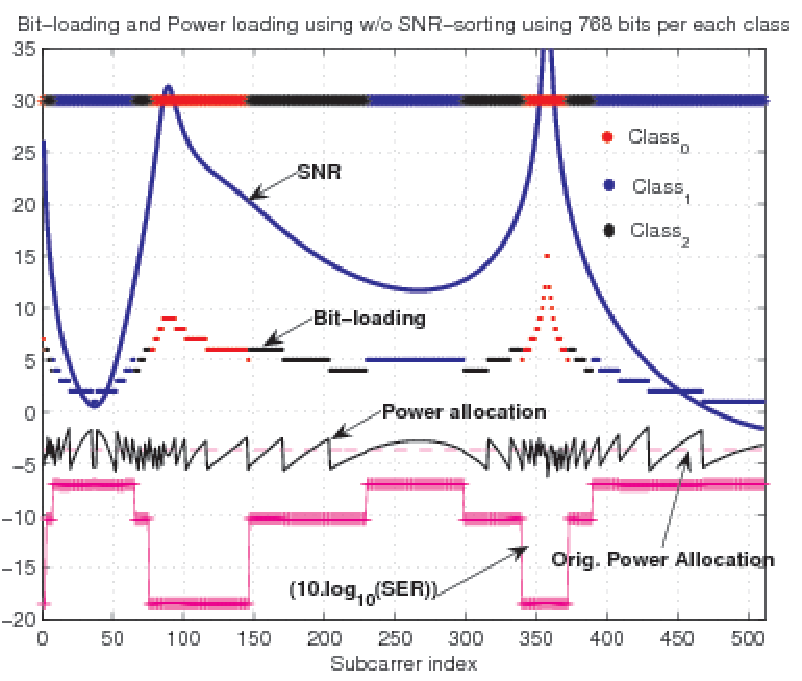
\includegraphics[width=7cm]{henkel_2}
  \caption{UEP bit and power allocation for three protection classes}
%  \caption{UEP bit and power allocation for three protection classes}
  \label{fig:henkel_2}
\end{figure}

\newpage
\paragraph{Organization}
% list the (research) events you have organized, if any,

\begin{enumerate}
\item Program Committee member of ICC 2006
\end{enumerate}

%\paragraph{Collaborations}
%\begin{enumerate}
%\item ...
%\item ...
%\item ...
%\end{enumerate}

\paragraph{Grants}
% list the running grants in 2005, if none have been received, please delete this
% subsection.
\begin{enumerate}
\item Funded by EU-IST STREP (FP 6), \emph{M-Pipe}, (October 2004
- March 2007)
\end{enumerate}

\paragraph{Patents}
\begin{enumerate}
\item  L. Sassatelli, W. Henkel, and D. Declercq. Check-Irregular LDPC Codes, Jan. 27
  2006. European Patent Application 06 100 979.1.
\item W. Henkel and K. Hassan. Unequal Error Protection Bit Loading for Multi-Carrier
  Transmission, Aug 30 2006. European Patent Application 06 119 771.1.
\end{enumerate}


%\paragraph{Publications}
% list the publications of 2005 (also accepted and in press), if none have been received, plese delete this
% subsection. Enter the publications into the SES publications database at
% http://kwarc.eecs.iu-bremen.de/ses-pubs/index.php and only reference them here.

%\begin{description}

%\item[Conference Proceedings]
  \nocite{Henkel_vDeetzen_IZS}
  \nocite{Hu_Henkel_Turbo}
  \nocite{Sassatelli_Henkel_Declercq_Turbo}
  \nocite{vDeetzen_Henkel_ISIT}
  \nocite{Henkel_Hassan_OFDM}
  \nocite{vDeetzen_ITG}
  \nocite{Hassan_Henkel_ITG}
%\item[Patents]
%  \nocite{Sassatelli_Henkel_Declercq_EP}
%  \nocite{Henkel_Hassan_EP}
%\end{description}

%%% Local Variables:
%%% mode: latex
%%% TeX-master: "report"
%%% End:

  \putbib[combined]
\end{bibunit}
{\noheader
\begin{bibunit}[hplain]
  \subsubsection{Harmonic Analysis applied to Communications
               Engineering}\label{ict:pfander}
               \index{Pfander, G\"otz}

\paragraph{Research Team}
G\"{o}tz Pfander (Professor), Niklas Grip (Postdoctoral Fellow)\\

%%% give a very short (150 words description of your research area)

In Multi-Carrier Modulation (MCM) communication schemes, the
channel input signal is synthesized as a linear combination
(superposition) of certain basis functions whose coeffcients
(weights) are bearing digital information. The performance of an
MCM system depends largely on the choice of the basis functions
which should allow the receiver to perform a fast and reliable
recovery of the transmitted information from the channel output.

For years, Orthogonal Frequency Division Multiplexing (OFDM) has
dominated MCM transmission systems, originally in time invariant
environments as in DSL applications but more recently also in slowly
time varying channels. The reason for this lies in the fact that, in
the stationary set-up, the OFDM carrier signals are approximate
eigenfunctions of the channel operator.

Mathematically, or more precisely, within harmonic analysis, OFDM
has been extensively studied under the disguise of Gabor analysis,
where stability issues, synthesis and analysis algorithms, and
carrier functions design are discussed at length (see also
Section~\ref{mps:pfander}).


\paragraph{Highlights}

In recent years, we have applied Gabor analysis to provide
mathematical contributions to MCM communications. For example, we
have shown that Gabor systems (OFDM, DMT) clearly outperform wavelet
systems (DWMT) in time invariant channels and we have analyzed
estimates of the crest factor of trigonometric polynomials which
underly OFDM.

In mobile and therefore wireless and time variant communication
environments, the transmitted signal reaches the receiver along a
continuum of different signal paths, each featuring a path dependent
time delay and a frequency shift caused by the doppler effect.
Nevertheless, physical constraints imply that this time--frequency
dispersion of the transmission signal is of limited extent. Hence,
wireless channels can be modelled by operators, which are weighted
superpositions of time and frequency shifts occupying a limited
region, the so--called spreading support in the time--frequency
plane. The weight functions are the so--called spreading functions
which play a fundamental role in our research
(Section~\ref{mps:pfander}).

\null {\emph{Transmission Basis Design:}} Since Fall 2004, we are
working on a DFG funded project, whose aim is the mathematical
analysis and optimisation of coded orthogonal frequency division
multiplexing (COFDM) in view of transmission stability in wireless
and other time variant environments. One of the cornerstones of
this project is the analysis of the perturbation stability of
different bases when used in wireless channels.

 \begin{figure}[ht]
   \begin{center}
    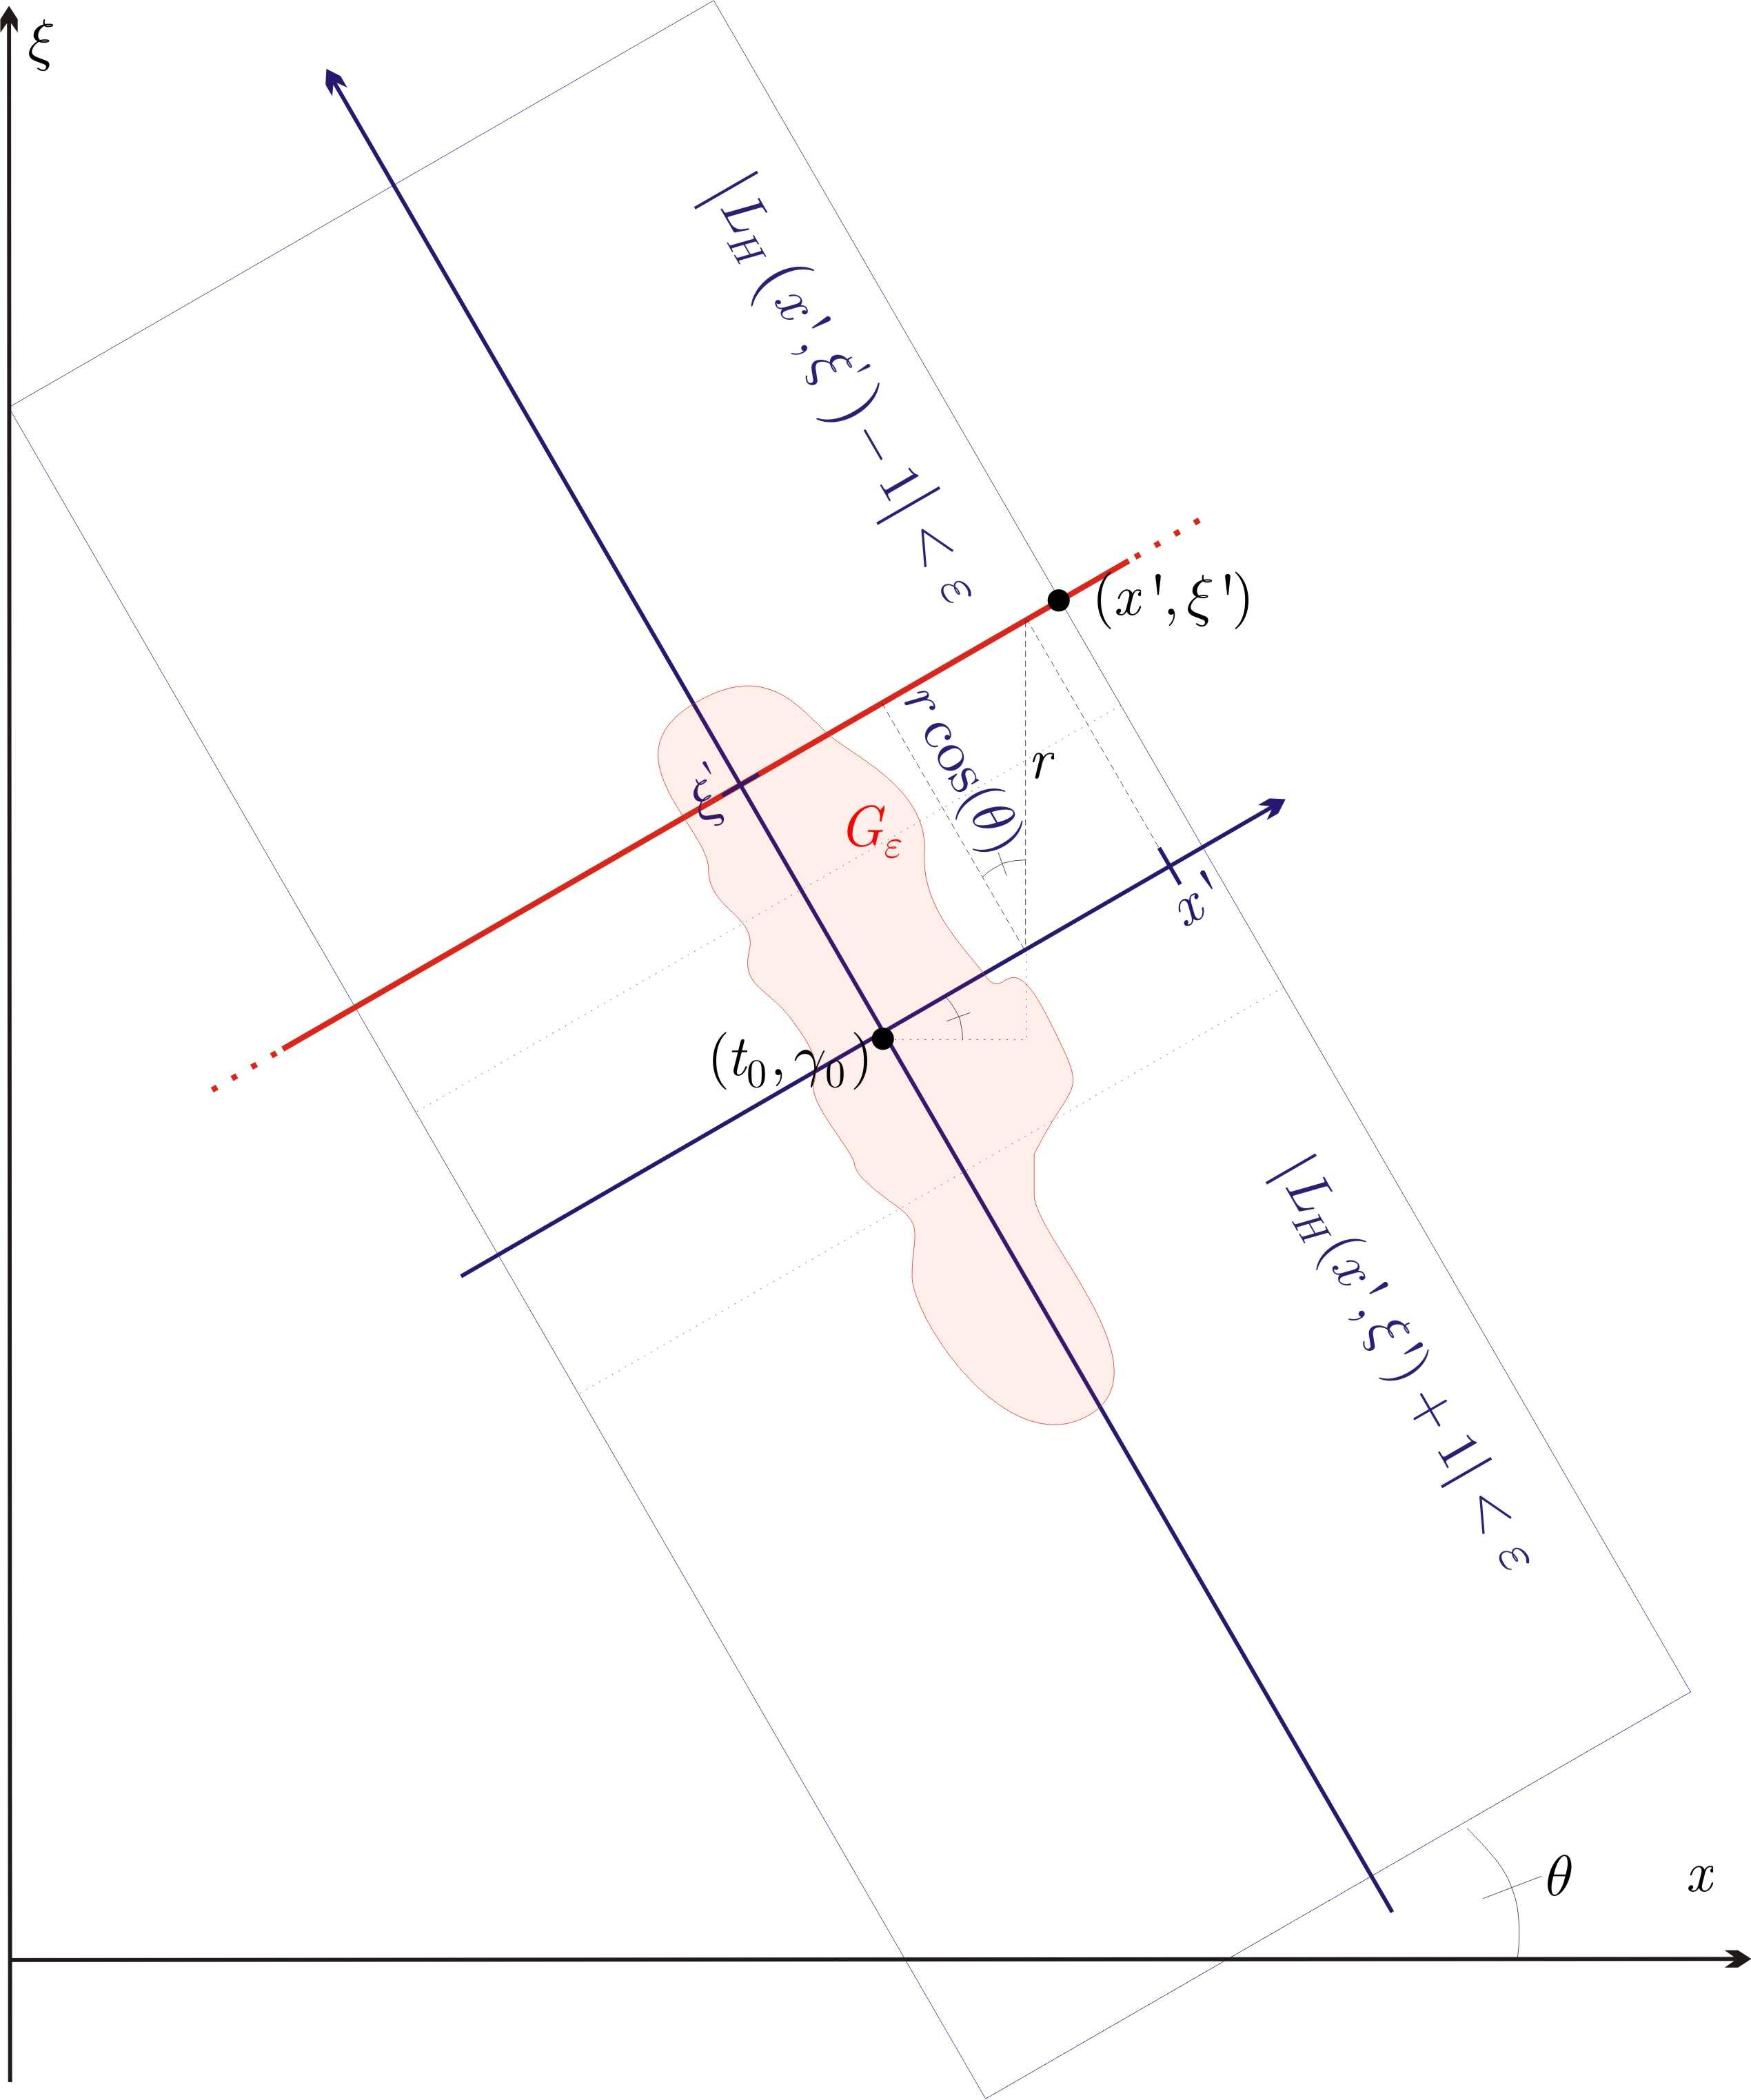
\includegraphics[width=7cm]{pfander.png}
     \caption{Construction of a channel spreading function whose operator causes a large distortion to a function
     with time--frequency $\epsilon$-support $G_\epsilon$.}
     \label{fig:pfander}
   \end{center}
 \end{figure}
% to reference it use ``Figure.~\ref{fig:xxx}''; the numbers will be computed automatically.

Within this realm, we derived estimates which relate the worst case
distortion of a function to the functions time--frequency
concentration and the channel operators spreading support (see
Figure~\ref{fig:pfander}). These results should, similarly to our
previous work on time invariant channels, allow us to show that OFDM
outperforms wavelet methods in mobile communication channels.

Further,  we continued our work on the modelling of narrowband
finite lifelength systems such as wireless radio communications by
smooth and compactly supported spreading functions. Our results were
used to derive a fast algorithm for computing the matrix
representation of a channel operator with respect to pulseshaped
OFDM bases \cite{GP06}.

\null {\emph{Operator/Channel Identification:}}  One of the key
problems in the design of elementary building blocks for mobile
communications is the incomplete knowledge of the ever--changing
transmission channels. The goal of operator/channel identification
is to obtain complete knowledge of a (channel-) operator by
observing the output caused by a single input signal.

Within the last years, we showed that classes of operators characterized by a bounded
spreading support region allow identification of its members if and only if the area of
the spreading support region is less than or equal to one, a phenomenon which is closely
related to Heisenberg's uncertainty principle~\cite{PW06,PW06b}. The theory, motivated by
communications engineering, has lead to the development of a sampling theory of operators
which is described in Section~\ref{mps:pfander}.

\null {\emph{Coding:}} Discrete, overcomplete Gabor systems can be
used to encode finite dimensional vectors in order to gain
robustness to errors introduced in  communications channels. In
\cite{KPR06}, we construct a large class of Gabor like equal norm
tight frames that are maximally robust to erasures. Further, we
discuss consequences of our findings to the theory of recovering and
storing signals which have sparse time--frequency representations.

%These results are further discussed in~\cite{KPR05}. The main
%focus of this paper are uncertainty principles for time--frequency
%representations of vectors in  finite dimensional vector spaces
%(Section~\ref{mps:pfander}).

%Possibly Channel matrix as picture
%
%% to include a figure, generate a file xxx.pdf and integrate the following lines
%\begin{figure}[ht]
%  \begin{center}
%   \includegraphics[width=10cm]{Pfander.pdf}
%    \caption{The caption of the figure}
%    \label{fig:xxx}
%  \end{center}
%\end{figure}
%% to reference it use ``Figure.~\ref{fig:xxx}''; the numbers will be computed automatically.
%
% Text ....
%
%
%\paragraph{Organization}
%% list the (research) events you have organized, if any,
%
%\begin{enumerate}
%\item  ....
%\item   ...
%\item  ...
%\end{enumerate}

\null G\"otz Pfander is also involved in  ``Applied Mathematics''
(Section~\ref{mps:pfander}).

\paragraph{Collaborations}
\begin{enumerate}
    \item {\sl International University Bremen}\\
          Prof. Harald Haas, Prof. Werner Henkel\\
          Design of OFDM systems for time--varying channels
    \item {\sl George Mason University, USA}\\
          Prof. David Walnut\\
          Operator sampling and channel measurements
    \item {\sl Numerical Harmonic Analysis Group and European Center
          for Time--Frequency Analysis, Vienna University, Austria}\\
          Prof. Hans Feichtinger, Prof. Karlheinz Gr\"ochenig\\
          Gabor analysis and applications to mobile communications
\end{enumerate}

\newpage
\paragraph{Grants}

\begin{enumerate}
    \item Funded by DFG, \emph {Analysis and design of COFDM multicarrier modulation techniques in view
          of transmission stability in time variant channels}, (September 2004 - December
          2006)
\end{enumerate}

%
%\paragraph{Patents}
%% list the grants you have received in 2005, if none have been received, plese delete this
%% subsection.
%\begin{enumerate}
%\item
%\item
%\end{enumerate}
%

%\paragraph{Awards, Prices}
%% list the grants you have received in 2005, if none have been received, plese delete this
%% subsection.
%\begin{enumerate}
%\item
%\item
%\end{enumerate}

%\paragraph{Publications}
% list the publications of 2005 (also accepted and in press), if none have been received, plese delete this
% subsection. Enter the publications into the SES publications database at
% http://kwarc.eecs.iu-bremen.de/ses-pubs/index.php and only reference them here.

%\begin{description}
 % \item[Journals]  Journal of Fourier Analysis and
 % Applications~
  %\nocite{LPW05,Pfa05}
 % \item[Submitted] IEEE Transactions on Information
%  Theory~
  %\nocite{PW051,GP05}
%\item[In preparation]
%\nocite{Pfa05b,KPR05}
%\end{description}


%\bibliographystyle{alpha}
%\bibliography{report-pfander-2005}

%\end{document}
%%% Local Variables:
%%% mode: latex
%%% TeX-master: "report"
%%% End:

  \putbib[combined]
\end{bibunit}
\begin{bibunit}[hplain]
  \subsubsection{Channel Characterization, Electromagnetics, Prototype System Development}
\index{Wallace, Jon}

\paragraph{Research Team}
Wallace, Jon (Professor)\\

Research combines the diverse areas of electromagnetics and
propagation, signal processing, and communications, to allow more
accurate modeling of realistic communications systems, revealing how
to optimize the performance of complex systems as a whole rather
than just the constituent parts.  This research involves a strong
experimental component, allowing results to be based on real-world
experiments and measurements and not just theoretical analysis. This
effort has led to the development of a number of prototype
multiple-input multiple-output (MIMO) wireless channel sounders and
the fabrication of RF/microwave antennas and components,
facilitating the development of accurate channel models and
revealing the impact of factors such as antenna mutual coupling,
directivity, and polarity. The work also encompasses the development
of real-time systems based on DSP and FPGA architectures for
implementing proposed communications algorithms as well as advanced
measurements techniques.

\paragraph{Highlights}

The work during 2006 has focused primarily on understanding the
complex behavior of time-varying MIMO wireless channels.  The rate
of time variation determines whether the MIMO communications channel
can be adequately tracked, allowing high throughput to be achieved
with the multiple antennas.

\begin{figure}[ht]
  \begin{center}
    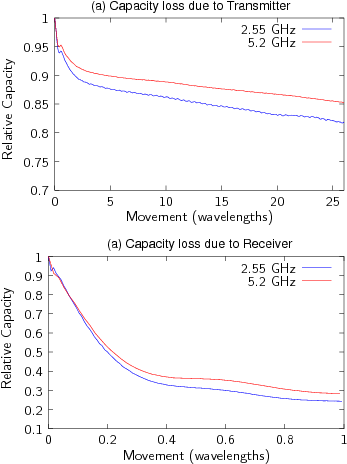
\includegraphics[width=6cm]{wallace_cap_deg.png}
    \caption{Capacity loss from time-varying channel with receiver
    movement due to channel errors at (a) transmitter and (b) receiver}
   \label{fig:wallace_cap_deg}
   \end{center}
\end{figure}

Measurement and analysis of time-varying channels in indoor and
outdoor environments at different frequencies revealed that for
moving users, the channel must be sampled at the receiver
approximately every 0.1 wavelength or shorter for high-capacity
communications, as depicted in Fig.~\ref{fig:wallace_cap_deg}.  It
was also found that channel information at the transmitter is less
critical and can be updated at the slower rate of every 1 wavelength
for high capacity.

This study on channel time-variation also led to metrics that quantify
the impact of the temporal variability as well as accurate methods of
capturing this behavior in computer simulations.  For very rapidly
fading channels (where learning the channel is not possible) it was
discovered that mutual coupling of the transmit array is a critical
factor affecting the system performance, and that not including
mutual coupling in the system model leads to erroneous conclusions
about the optimal configuration of the transmit antenna array.

\begin{figure}[ht]
  \begin{center}
    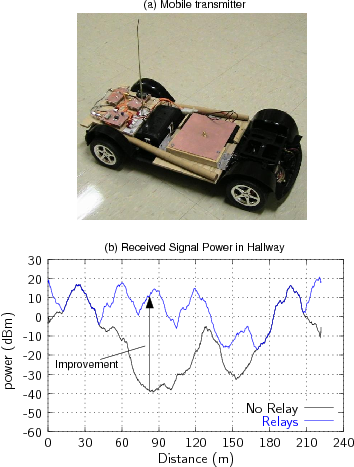
\includegraphics[width=6cm]{wallace_relay2.png}
    \caption{System for rapid shadowing/pathloss measurements and possible
    improvement using relays for a hallway environment}
   \label{fig:wallace_relays}
   \end{center}
\end{figure}

Additional channel modeling work done in collaboration with the
University of Pretoria, South Africa, has demonstrated interesting
properties of indoor propagation channels.  It has been discovered
that the multipath structure, antenna correlation, and channel
capacity are very similar, even when the center frequency is scaled.

Defense-related contract work  was done for San Diego Research
Corporation, USA, whose primary goal was to quantify how the
blockage (or shadowing) of electromagnetic signals in urban
environments limits communications reliability, and whether this
could be improved by robotic relays.  As depicted in
Fig.~\ref{fig:wallace_relays}, a transmitter operating at 300 MHz,
900 MHz, and 2 GHz, was mounted on a remote control car and the
signal strength was measured on a fixed receiver.  The car was
driven in many different scenarios: indoor hallway, indoor room,
outdoor-to-indoor channels, behind automobile, under automobile,
etc. Analysis of the resulting shadowing versus position revealed
that shadowing can cause a drop of 10-30 dB when going around a
corner or behind an automobile.  A simple daisy-chain relay model,
however, indicated that self-configuring robotic relays may be
effective in allowing reliable communications in these environments.


In the future, the main focus is  building up new experimental
capability for ultrawideband multiple antenna channel sounding and
cognitive radio, as well as forming collaborative relationships with
other key researchers in Germany and Europe.

%Pictures are to be included via:
%
%\begin{figure}[ht]
%  \begin{center}
%    \includegraphics[width=6cm]{profxxx-figx.jpg}
%    \mycaption{ xxx )}\label{fig:profxxx}
%   \end{center}
%\end{figure}

% \paragraph{Organization}
% list the (research) events you have organized, if any,
%
%\begin{enumerate}
%\item  xxx
%\item  xxx
%\end{enumerate}

 
\paragraph{Collaborations}
\begin{enumerate}
\item {\sl University of Pretoria, South Africa} \\ B. T. Maharaj and L. P. Linde \\ Indoor Channel Measurement and Modeling
%\item {\sl Institution} \\ Partner \\ Research Topic \ Collaboration
\end{enumerate}

%\paragraph{Grants}
%% list the running grants in 2005, if none have been received, please delete this
%% subsection.
%\begin{enumerate}
%\item {Funded by} ``Proposal ��
%\item {Funded by} ``Proposal ��
%\end{enumerate}

%\paragraph{Awards, Prizes}
%% list the grants you have received in 2005, if none have been received, please delete this
%% subsection.
%\begin{enumerate}
%\item
%\item
%\end{enumerate}

%\paragraph{Publications}
  \nocite{wallace_06bWALa,wallace_069WAL,wallace_06bWALb}

%Publications should be delivered as a separate file (naming
%convention profxxx.bib. See description by R. Helling. Please make
%sure that all your publications are referred to in the TiX file.
%This can either be in form of a \cite{profxxxkey} or as a
%\nocite{profxxxkey} in the end. A publication which is not
%reffered to on the LaTeX file doesn't produce any output in the
%report.

  \putbib[combined]
\end{bibunit}
\shorttitle{Smart Systems}
\subsection{Smart Systems}
As humans we can sense, act, speak, listen, decide and sometimes
understand.  The 21st century will witness technologies that can do
the same. 
Robots are for example more and more used in domains where some autonomy and 
intelligence is necessary. They work under conditions where the robot is 
not constantly supervised by a human operator and where it has to be 
adaptive as its developer can not fully predict which situations it will 
encounter in its application environment. 
But also information services are rapidly changing from 
statically served data to information that is dynamically tailored to each individual user's
current needs. This information is fetched instantaneously from networked, distributed sources which
themselves change and evolve continually. At the same time, new representation formats
allow to discover and specify the internal and functional structure of information and
drive services that previously required (human) understanding. Technically, we observe the
convergence of databases, Internet, and distributed systems into semantically enriched
knowledge systems which allow the casual as well as the professional user to deal with the
ever-growing amount of information available.  
Another issue is the presentation of
information to the user.  Data visualization is concerned with the management of large
data, the filtering and extraction of salient features, and their visual representation in
an expressive, intuitive, and interactive manner.

%%% Local Variables:
%%% mode: latex
%%% TeX-master: "report"
%%% End:

\begin{bibunit}[hplain]
  \newpage
\subsubsection{Reasoning, Semantics, and Knowledge  Management}
\label{ict:modeling:kohlhase} \index{Kohlhase, Michael}

\paragraph{Research Team}
Michael Kohlhase (Professor),
Heinrich Stamerjohanns (Head of CS Labs, see~\ref{ict:stamer}),
Christoph Lange (PhD Student),
Christine M\"uller (PhD Student),
Normen M\"uller (PhD Student),
Immanuel Normann (PhD Student),
Florian Rabe (PhD Student),
Andrea Kohlhase (Research Programmer) \\

%%% give a very short (150 words description of your research area)
%% Hint: this can be copied from the research areas document (../masterplan/research-areas)

The ability to represent knowledge about the world and to draw logical inferences is one
of the central components of intelligent behavior, as a consequence, reasoning components
of some form are at the heart of many artificial intelligence systems.

The work of the KWARC (\underline{K}no\underline{w}ledge \underline{A}daptation and
\underline{R}easoning for \underline{C}ontent) group centers around building knowledge
management systems for e-science applications, in particular for the natural and
mathematical sciences.  The main assumption in this work is that if the structure of the
factual content of scientific documents, their contributions and dependencies regarding a
larger knowledge context is made sufficiently explicit, then this structure becomes
amenable to machine manipulation. Thus high-level added-value (web)-services can be offered,
e.g. semantic search and navigation (independent of the surface presentation),
user-adaptive presentation and content tailoring, and extended semantic quality control up
to proof verification.

\paragraph{Highlights}

%%% give a short (500 words)description of the research highlights. 1 figure costs 100 words
The highlight in 2006 was the publication of a 500 page book on OMDoc in the Springer
Lecture Notes in Artificial Intelligence series~\cite{Kohlhase:omdoc1.2}. OMDoc
({\underline{O}}pen {\underline{M}}athematical {\underline{Doc}}uments) is an
{\sc{Xml}}-based representation format for mathematical knowledge developed in the KWARC
group. This format is used in various ($\geq 10$) international projects as the knowledge
representation base.

\begin{figure}[ht]
\begin{center}
  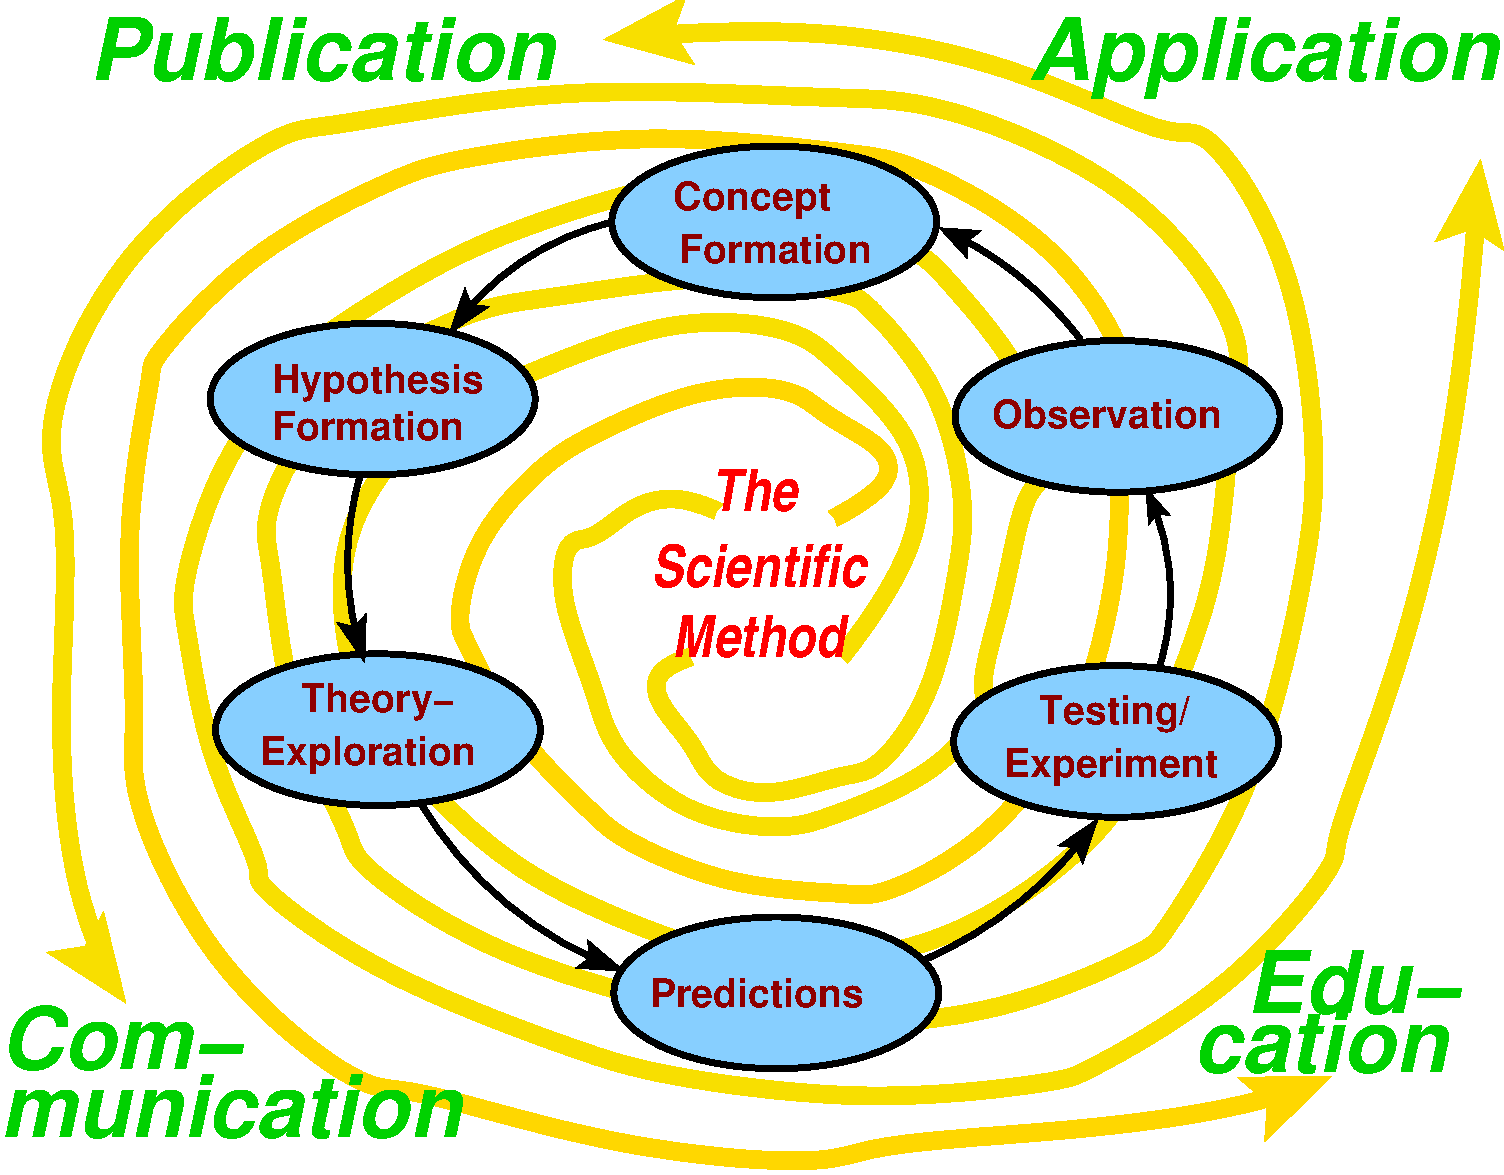
\includegraphics[width=7cm]{sci-method}
\end{center}
\caption{The Spiral View of Scientific Method}\label{fig:nw-Methode}
\end{figure}

We have extended the knowledge representation infrastructure in OMDoc to other topics in
the natural sciences to make it into a general semantic representation language that
supports seamless computer support in a ``{\emph{Scientific Semantic
    Web}}''~\cite{HilKohSta:copmem06}. Our starting point is the view of the
{\emph{scientific method}} as a spiral (Fig.~\ref{fig:nw-Methode}). In this view,
scientific research moves in a spiral trajectory from original ideas to results and
applications. At the moment, most of the steps in Fig.~\ref{fig:nw-Methode} are separately
supported by software systems, e.g. literature searches in Google Scholar or Wikipedia,
theory exploration in computer algebra systems and experiments in simulation systems. But
the systems are, largely, not able to inter-operate since they use differing data formats,
make differing model assumptions, and are bound to an implicitly given context that is
only documented in publications about the systems. A joint and universally applicable
representation language will be an enabling technology that alleviates these problems.

To make this vision come true, we have developed
\begin{enumerate}
\item a highly efficient, content-based document retrieval engine for
  mathematics~\cite{KohSuc:asemf06},
\item an OMDoc-based semantic WIKI~\cite{LanKoh:swim06,LanKoh:swmkm06,lange06:wikiblog},
\item a theoretical foundation for invasive editors and implementations in the MS Office
  suite~\cite{Kohlhase:UserAsPrisoner,Kohlhase:MediaOrMedeaSociety,Kohlhase:emPowerPoint},
\item methods for the discovery of theory morphisms in mathematical
  libraries~\cite{Normann:etrpti06}
\item a methodology for an ontology-based management of
  change~\cite{NRM:omdoc2vf06,Mueller06:locutor-lwa}, and
\item a representation format for logical systems with logic morphisms and
  proofs~\cite{rabe:dfol:06,rabe:moloss:06}
\end{enumerate}
We have started a research group of undergraduate CS students that undertake the
translation of the Cornell EPrint Archive from {\LaTeX} to XHTML+MathML (we can currently
translate 45\% of 400.000 articles in Physics, Mathematics, Computational Biology, and
Computer Science). This corpus will subjected of a semantic analysis with computational
linguistics methods and will be the basis of scalability studies for the methods and
representation formats presented above.

\paragraph{Organization}

In 2006, Prof. Michael Kohlhase was
\begin{enumerate}
\item Program and Conference Co-Chair of the 29.th Annual German Conference on Artificial
  Intelligence KI'06\cite{KI06}
\item Trustee of the Conference on Automated Deduction
\item Trustee of the Mathematical Knowledge Management Interest Group
\item Trustee of the CALCULEMUS Interest Group
\item Member of the Executive Committee of the OpenMath Society
\item Member of the MathML Working Group of the World Wide Web Consortium (W3C)
\item Member of 11 Program Committees of International Conferences.
\item Member of the Reviewer's College of the Engineering and Physical Sciences Review
  Research Council (EPSRC)
\item General Editor ``QPQ: an Online Journal for Peer-Reviewed Deductive Software
  Components'' {\url{http://www.qpq.org}}
\item Editor ``Journal of Applied Logic'', Elsevier.
\item Member of the ``Auswahlausschu\ss der Studienstiftung des Deutschen Volkes''
\end{enumerate}

\paragraph{Collaborations}
Prof. Michael Kohlhase is a Vice Director of the ``Safe and Secure Cognitive Systems'' of
the newly founded Department of the German Research Institute Lab Bremen. This leads to an
intensive collaboration of the KWARC group with this research group, which includes joint
projects and supervision of students. Further collaborations of the KWARC group include
\begin{enumerate}
    \item {\sl Rice University, USA}\\
          Prof. Richard Baraniuk\\
          Extending the Connexions Representation Format CNXML
    \item {\sl National Institute of Standards, USA}\\
          Dr. Bruce Miller\\
          Transforming {\LaTeX} documents to OMDoc/CNXML
    \item {\sl International University Bremen}\\
          Prof. Peter Baumann\\
          Extending OMDoc to GIS-Data/Living Documents
    \item {\sl Institute for Science Networking}\\
          Prof. Eberhard R. Hilf\\
          Extending OMDoc to PhysML
    \item {\sl Carnegie Mellon University, USA}\\
          Prof. Frank Pfenning, Prof. Peter Andrews\\
          Higher-Order Theorem Proving and Meta-Logical Frameworks
    \item {\sl Universit\"at des Saarlandes}\\
          Prof. J\"org Siekmann, Dr. Christoph Benzm\"uller\\
          Higher-Order Theorem Proving
    \item {\sl Deusches Forschungszentrum f\"ur K\"unstliche Intelligenz, Saarbr\"ucken}\\
          Dr. Dieter Hutter\\
          Ontology-based Management of Change
    \item {\sl Design Science Inc.}\\
          Dr. Robert Miner\\
          Mathematical Document Retrieval
\end{enumerate}

% \paragraph{Awards, Prizes}
% % list the awards, prizes you have received in 2005, if none have been received, plese delete this
% % subsection.
% \begin{enumerate}
% \item DAAD, grant for a year at Carnegie Mellon University.
% \end{enumerate}

\paragraph{Grants}
% list the running grants in 2005, if none have been received, please delete this
% subsection.
\begin{enumerate}
\item Funded by EU-IST (FP 6), \emph{ ONCE-CS}, (July 2005 -
December 2007)
\\
\item Funded by EU-IST (FP 6) \emph{JEM}, (July 2006 - July 2009)

%\item Industry: Design Science Inc. Grant for transforming Cornell Eprint archive.
\end{enumerate}

%\paragraph{Publications}
\nocite{BenBroKoh:csil06}
%\end{document}
%%% Local Variables:
%%% mode: latex
%%% TeX-master: "report"
%%% End:

% LocalWords:  Stamerjohanns EECS uller Normen Normann Rabe KWARC daptation Xml
% LocalWords:  easoning ontent OMDoc athematical uments Google Baraniuk CNXML
% LocalWords:  Baumann GIS Hilf Pfenning Universit des Saarlandes org Siekmann
% LocalWords:  Benzm Krieg uckner Deusches

  \putbib[combined]
\end{bibunit}
}
\begin{bibunit}[hplain]
  
\subsubsection{Simulation and Control of Complex Dynamical Systems}\label{ict:modeling:antoulas}
\index{Antoulas, A.C.}

\paragraph{Research Team}
Athanosios Antoulas (Professor)

Model reduction seeks to replace a large-scale system of differential
or difference equations (the outcome of discretizing a PDE, perhaps) by a
system of substantially lower dimension, that ideally, has the same
response characteristics as the original system,
yet requires far less computational resources for realization than the
potentially unmanageable levels that may be required by the larger original
system.

Two main currents can be identified among methodologies for model reduction.
Balanced approximation methods are built upon a family of
ideas with very close connection to the singular value decomposition.
These methods preserve stability and allow for global error bounds but
often do not scale well in terms of
computational efficiency and stability when applied to large scale problems.
Moment matching methods are based principally on Pad\'e-like
approximations and for large-scale problems have lead naturally to the
use of Krylov and rational Krylov subspace methods. These methods generally
enjoy greater efficiency  and numerical stability.
A strong current trend aims at combining these two approaches by deriving
iterative methods which achieve approximate balanced reduction.

\paragraph{Highlights}

%%% give a short (500 words)description of the research highlights. 1 figure costs 100 words

% to include a figure, generate a file xxx.pdf and integrate the following lines
%% \begin{figure}[ht]
%%   \begin{center}
%%     \includegraphics[width=10cm]{xxx}
%%     \caption{The caption of the figure}
%%     \label{fig:xxx}
%%   \end{center}
%% \end{figure}
% to reference it use ``Figure.~\ref{fig:xxx}''; the numbers will be computed automatically.

Our research activities are concerned with the circle of ideas surrounding
model reduction. It provides efficient
and robust methods for producing reduced order models of
large state space systems.  These activities
have an impact both in system theory of complex systems
as well as in applied mathematics and in particular numerical methods for
large-scale problems.  Once the theory and computational
methods are developed, we expect that high quality software will result and
have applications in many areas of engineering.
This will enable at a later stage,
the design of real time controllers for complex systems.

{\it Broader impact resulting from the proposed activities}.
In today's technological world, physical processes are
described mainly by mathematical models, which are used to
simulate the behavior of the physical processes in question.
Sometimes, they are also used to modify or control their behavior.
In this framework, there is an ever increasing need for
improved accuracy which leads to models of high complexity.

The basic motivation for system approximation is the need in many
instances for a simplified model of a dynamical system, which
however captures the main features of the original complex model.
This need arises from limited computational, accuracy, and storage
capabilities. The simplified model is then used in place of the
original complex model, either for {\it simulation}, or {\it control}.

Important areas of application of model reduction are: VLSI
(Very Large Scale Integration) design, weather prediction,
air quality management, molecular dynamics simulations, simulation and
control of chemical (e.g. CVD - Chemical Vapor Deposition) reactors,
car windscreen quality management, simulation and control of MEMS (Micro
Electro Mechanical Systems) devices, e.g. micromirrors, to name but a few.
Thus the proposed activities have potential benefits for society at large.

%\paragraph{Organization}
% list the (research) events you have organized, if any,

%\begin{enumerate}
%\item  ....
%\item   ...
%\item  ...
%\end{enumerate}

%\paragraph{Collaborations}
%\begin{enumerate}
%\item ...
%\item ...
%\item ...
%\end{enumerate}

\paragraph{Grants at RICE University}
% list the running grants in 2005, if none have been received, please delete this
% subsection.
\begin{enumerate}
\item
Funded by US National Science Foundation, R38570-776000, NSF CCR-0306503, \emph {Model
  Reduction for Structured Dynamical Systems}, (August 2003 - July 2006)
% Amount: \$$436,607.00$ 

\item
Funded by US National Science Foundation,  ITR (Information Technology Research) Grant,
collaborative with Purdue and Florida State, R38670-776000, NSF ACI-0325081, \emph
{Research on Model Reduction of Dynamical Systems for Real-time Control}, (January 2003 -
August 2007)
      %Amount: \$$1,826,959.00$\\

\item
Funded by US National Science Foundation, OSR No.: 06052204, NSF CCF-0634902,
\emph{Advanced Projection Techniques for Dimension Reduction of Large Scale Dynamical
  Systems}, (October 2006 - September 2009)

\end{enumerate}

%\paragraph{Patents}
% list the grants you have received in 2005, if none have been received, plese delete this
% subsection.
%\begin{enumerate}
%\item
%\item
%\end{enumerate}


%\paragraph{Awards, Prices}
% list the grants you have received in 2005, if none have been received, plese delete this
% subsection.
%\begin{enumerate}
%\item
%\item
%\end{enumerate}

%\paragraph{Publications}
% list the publications of 2005 (also accepted and in press), if none have been received, plese delete this
% subsection. Enter the publications into the SES publications database at
% http://kwarc.eecs.iu-bremen.de/ses-pubs/index.php and only reference them here.
\nocite{aca1}

% \begin{description}
% \item[Book]
% A.C. Antoulas,
% ``Approximation of large-scale dynamical systems'',
% Book Series: {\it Advances in Design and Control} {\bf DC 06}, 479 pages,
% SIAM, Philadelpia (2005).
% \item[Journal Paper]
% D.C. Sorensen and A.C. Antoulas,
% {\it On model reduction of structured systems}, in
% "Dimension Reduction of Large-Scale Systems",
% Edited by P. Benner, V, Mehrmann and D.C. Sorensen,
% Springer Verlag, pages 125-138, (2005).
% \item A.C. Antoulas, {\it A new result on passivity preserving
% model reduction}, Systems and Control Letters,
% Volume 54, Issue 4, Pages 361-374, April (2005).
% \item[Journal Paper]
% S. Gugercin and A.C. Antoulas,
% {\it Model reduction of large-scale systems by least squares},
% Linear Algebra and Applications,
% Special Issue on Order Reduction of Large-Scale Systems,
% Edited by P. Benner, D.C. Sorensen, R. Freund, and A. Varga, accepted
% for publication, 2005.
% \item[Journal Paper]
% A.C. Antoulas, {\it Frequency domain representation and singular
% value decomposition}, UNESCO EOLSS (Encyclopedia for the Life Sciences),
% Contribution 6.43.13.4, 52 pages, in press, 2005.
% \item[Journal Paper]
% A.C. Antoulas, {\it An overview of model reduction methods for large-scale
% dynamical systems}, IFAC Annual Reviews in Control, Invited Paper,
% JARAP vol. {\bf 228} (2005).
% \item[Report]
% Q. Zhou, K. Mohanram, and A.C. Antoulas,
% {\it Structure Preserving Reduction of Frequency-dependent Interconnect},
% Technical Report, June (2005).
% \item[Journal Paper]
% A.C. Antoulas, E. Gildin, R.H. Bishop and D.C. Sorensen,
% {\it Model and controller reduction for seismically excited buildings},
% submitted to "Structural Control and Monitoring", November (2005).
% \item[Journal Paper]
% S. Gugercin, A.C. Antoulas, and C. Beattie, Technical Report,
% {\it An iterative rational Krylov approach to optimal H2 model reduction},
% SIMAX (SIAM J. Matrix Analysis and Applications), 2006 (submitted).
% \item[Journal Paper]
% A.J. Mayo and A.C. Antoulas,
% {\it A framework for the general realization problem},
% {Linear Algebra and Its Applications}, Special Issue in honor of P.A. Fuhrmann,
% Edited by A.C. Antoulas, U. Helmke, J. Rosenthal, V. Vinnikov, and E. Zerz.
% 2006 (sumbitted).
% \item[Journal Paper]
% S. Gugercin, A.C. Antoulas, and C.A. Beattie,
% {\it Krylov-based controller reduction for large-scale systems},
% {Automatica}, 2006 (submitted).
%\end{description}
%%\end{document}
%%% Local Variables:
%%% mode: latex
%%% TeX-master: "report"
%%% End:

  \putbib[combined]
\end{bibunit}
\begin{bibunit}[hplain]
  \subsubsection{Raster Data Services}
\index{Baumann, Peter}
\paragraph{Research Team}
Peter Baumann (Professor), Angelica Garcia Gutierrez (PhD Student)\\

Raster data occur in various dimensions, be they observed phenomena or generated data
sets. Examples comprise satellite imagery and mapping, geo physics and exploration,
medical imagery, engineering data, and statistics data. A key property they have in common
is their extreme volumes, often Giga- to Petabyte per object.

With the advent of sufficiently large disk capacities data providers more and more tend to
publish such large Multidimensional Discrete Data (MDD) - GoogleEarth is a prominent
example. Generally such services are implemented in an ad-hoc manner, and consequently
offer limited functionality (such as GoogleEarth: zoom and pan on satellite
maps). However, flexible, value-added data navigation and analysis requires more, both for
experts (such as exploration engineers) and the general public (where internally complex
functionality like local weather prediction obviously should be wrapped for easy access).

MDD database and Web service support raises new questions on all levels: conceptually,
formal models are needed to describe data and services; query languages resp. request
interfaces need to be designed based on these foundations. Efficient implementation,
including optimizing query evaluation and storage structures, is needed. The high volume
suggests to include tape robots as nearline storage facilities. Last but not least
services for as many application domains as possible need to be realized to gain domain
understanding and to evaluate service implementations.

In our research we investigate on the principles of MDD management based on the rasdaman
("raster data manager") system acting as a research platform. Application domains
inspected are mainly stemming from earth system research, such as 2-D to 4-D remote
sensing, exploration, marine, and climate data. As a byproduct we are actively engaged in
the Open GeoSpatial Consortium where we contribute to the standardization of geo raster
services.

\paragraph{Highlights}

An important work package is contribution to geo raster service
standardization in the Open GeoSpatial Consortium (OGC,
\url{http://www.opengis.org}). We are actively contributing in the
Web Coverage Service (WCS) Revision Working Group where the
substantially revised WCS version 1.1 has been finished by the end
of 2006. Based on the experience gained there and the WCS
shortcomings spotted we have propose the concept of a Web Coverage
Processing Service (WCPS); Figure~\ref{fig:ndvi} exemplifies usage
of WCPS by dynamically deriving the NDVI of a Landsat satellite
scene; the NDVI I of an image is defined as I=(nir-red)/(nir+red),
in the right image it is thresholded as $I>0.6$. In June 2006, WCPS
has been lifted to a Best Practice Paper (which implies OGC
endorsement), it is estimated that WCPS can become a Draft Standard
end of 2006 / beginning of 2007, and a full standard by summer 2007.
Several institutions, among them German mapping (AdV) and
geophysical institutions (such as BGR) have expressed their
interest.

In parallel to the conceptual work on WCS and WCPS, our group implements both
services. Prototypes have been demonstrated at various occasions in 2006, among them OGC
Technical Commitee meetings. For 2007 it is planned to set up large-scale services fo
thorough evaluation prior to freezing the final standard document.

The GALEON (Geo-interface to Atmosphere, Land, Earth, Ocean, NetCDF) project launched in
2005 meantime has become an OGCnetwork (\url{http://www.ogcnetwork.net/galeon}); besides
contributing to WCS requirements it is starting now to hands-on evaluate the new WCS
1.1. IUB will contribute our WCS implementation, which is under work,

As part of the IRCCM project (\url{http://www.irccm.org}) and in collaboration with IUB's geo group and
AWI Bremerhaven, a standards-based open service for marine research data has been set up
which combines bathymetry data and video mosaics acquired by a French underwater
robot. Data describe an underwater volcano in the Norwegian Atlantic area known as
Hakon-Mosby. This service is the first step towards a more comprehensive multi-sensor
fusion service between IUB and AWI.

For the ICSU CODATA (Committee on Data in Science and Technology) a German section has
been established as an "e.V." and has been accredited with CODATA International. As a side
effect of this work, several fruitful research contacts have emerged, such as with the
Chinese Academy of Science (see above).

\begin{figure}[ht]
  \begin{center}
     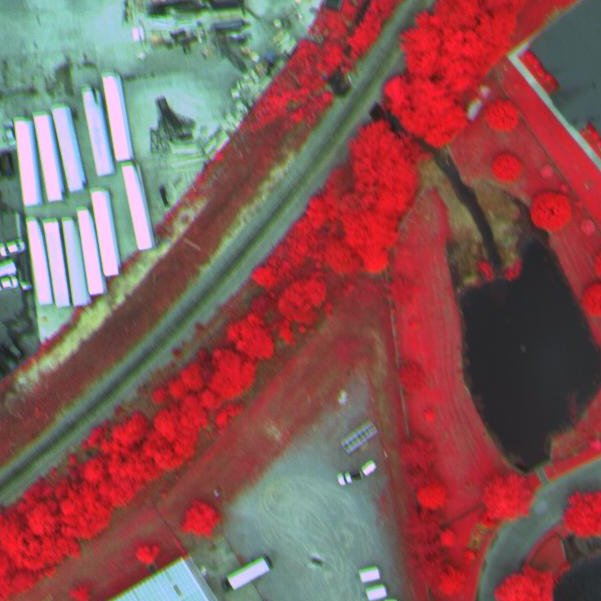
\includegraphics[width=3.5cm]{ndvi-1.jpg}
     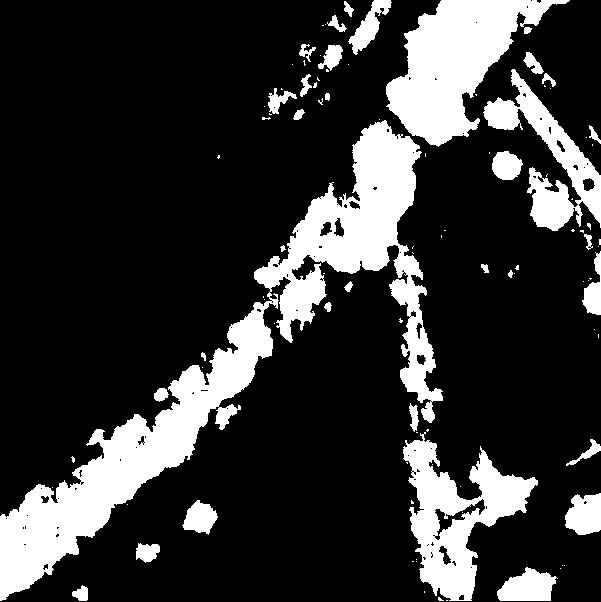
\includegraphics[width=3.5cm]{ndvi-2.jpg}
    \caption{The Normalized Difference Vegetation Index (NDVI) as a database / Web
      service query (rasdaman screen shots).}\label{fig:ndvi}
   \end{center}
\end{figure}

\paragraph{Collaborations}

In 2006 several new international research cooperations have been established:
\begin{enumerate}
\item {\sl Universidade de Campinas (Unicamp), Campinas, Brazil}

  Prof. Claudia Bauzer Medeiros is Head of the Laboratory of Information Systems (LIS) at
  the Institute of Computing, UniCamp, and President of the Brazilian Computer
  Society. With her group she works on advanced Web-based geo services with emphasis on
  agrocultural and environmental applications; to this end there is a long-standing
  relation with the Brazilian Ministry of Agriculture.

  In the collaboration, for which a joint research proposal has been submitted to
  DAAD/Germany and INPe/Brazil, both partners plan to extend Unicamp's geo services with
  IUB's raster services, based on the open OGC standards. The resulting system will be
  exercised in real life operation. Evaluation results will be brought into OGC to give
  feedback to the standards developers.

\item {\sl Universidad de Sinaloa, Sinaloa, Mexico}

  Dr. Ines Fernando Lopez Vega, who in 2004 has received his PhD from University of
  Arizona at Tucson, is building up his research on image time series
  evaluation. Collaboration is foreseen combining his interests with our raster service
  research and Michael Kohlhase's work on Semantic Web services.

  Collaboration was initiated in Fall 2006 with a visit of Dr Lopez Vega in the course of
  his co-supervision of Angelica Garcia Gutierrez's PhD work.

\item {\sl Chinese Academy of Sciences and Jilin University, Changchun, China}

  Prof. Liu Chuang plays an important role in China when it comes to provision and
  exploration of remote sensing data. Among others, she is Vice Director of the Institute
  of Geography and Natural Resources (IGNR) and director of the Spatial Data Commission,
  the Chinese Association of Geographic Information System (CAGIS), and Secretary General
  of a Working Group of Remote Sensing and Data Information Systems (RS/DIS).

  IUB, IGNR und Jilin University plan joint activities in the field of open
  standards-based geo services on high-volume in situ and remote sensing data, based on
  rasdaman. As a real life application IGNR's 100+ TB data archive of Chinese satellite
  imagery collected over several years will serve, today stored in hundreds of DVDs,
  unavailable to the researcher community. The Chinese National Disaster Reduction Center
  will be one of the first users, with application scenarions being river floods and
  earthquakes.
\end{enumerate}


Several tutorials have been given on the topic of raster services:
\begin{enumerate}
\item CODATA 2006 Conference, Beijing (3 hrs)
\item 1st International Symposium on Cooperation and Promotion of Information Resources in
  Science and Technology (under the auspices of the Chinese Ministry of Science and
  Technology), Beijing (2 hrs)
\item 19th IFIP World Computer Congress, Santiago de Chile (3 hrs)
\end{enumerate}

%\paragraph{Publications}

%\begin{description}
\nocite{PB:comogis,PB:codata,PB:fig}
%\end{description}
%%% Local Variables:
%%% mode: latex
%%% TeX-master: "report"
%%% End:

  \putbib[combined]
\end{bibunit}
\begin{bibunit}[hplain]
  %\svnInfo $Id$
%\svnKeyword $HeadURL$

%\documentclass{article}
%\usepackage{epsfig}
%\begin{document}

\subsubsection{Visualization and Computer Graphics}
\index{Linsen, Lars}

\paragraph{Research Team}
Lars Linsen (Professor),
Sherin Al-Shbat (PhD Student),
Tetyana Ivanovska (PhD Student),
Tran Van Long (PhD Student),
Paul Rosenthal (PhD Student)\\

The Visualization and Computer Graphics Laboratory (VGCL) led by Prof.~Lars Linsen is
mainly concerned with topics from scientific and information visualization plus some
selected topics from computer graphics and geometric modeling.

Visualization is an inherently interdisciplinary field with application in many different
areas.  Scientific visualization deals with the visualization of data with spatial
interpretation such as computer-generated data from numerical simulations (physics,
chemistry) or measured data using scanning or sensoring techniques (medicine, life
sciences, geosciences).  The group's efforts are to generate visualization methods that
can handle large data sets efficiently, filter distinct features automatically or
interactively, and display the relevant information in a comprehensive and intuitive
fashion.  The research focuses on segmentation and isosurface extraction, hierarchical
methods, multi-variate data visualization, flow and tensor field visualization, and user
interaction.

Information visualization deals with the visualization of abstract data with no spatial
interpretation such as graph- or network-based data (life sciences, social sciences) or
multi-dimensional data (databases, ecomomics).  The group's efforts focus on interactive
exploration and analysis tools for such abstract data.

In the areas of computer graphics and geometric modeling the group's interest lies in
point-based methods, multi-resolution surface representation, and curves on surfaces.


\paragraph{Highlights} \ \\

{\em Direct Isosurface Extraction from Scattered Volume Data.}
Isosurface extraction is a standard visualization method for scalar volume data and has
been subject to research for decades.  Nevertheless, no isosurface extraction method
existed that directly extracts surfaces from scattered volume data without 3D mesh
generation or reconstruction over a structured grid. We have developed a method based on
spatial domain partitioning using a $k$d-tree and an indexing scheme for efficient
neighbor search. Our approach consists of a geometry extraction and a rendering step. The
geometry extraction step computes points on the isosurface by linearly interpolating
between neighboring pairs of samples. The neighbor information is retrieved by
partitioning the 3D domain into cells using a $k$d-tree. The cells are merely described by
their index and bitwise index operations allow for a fast determination of potential
neighbors. The final rendering step uses point-based rendering techniques.

\begin{figure}[ht]
  \begin{center}
    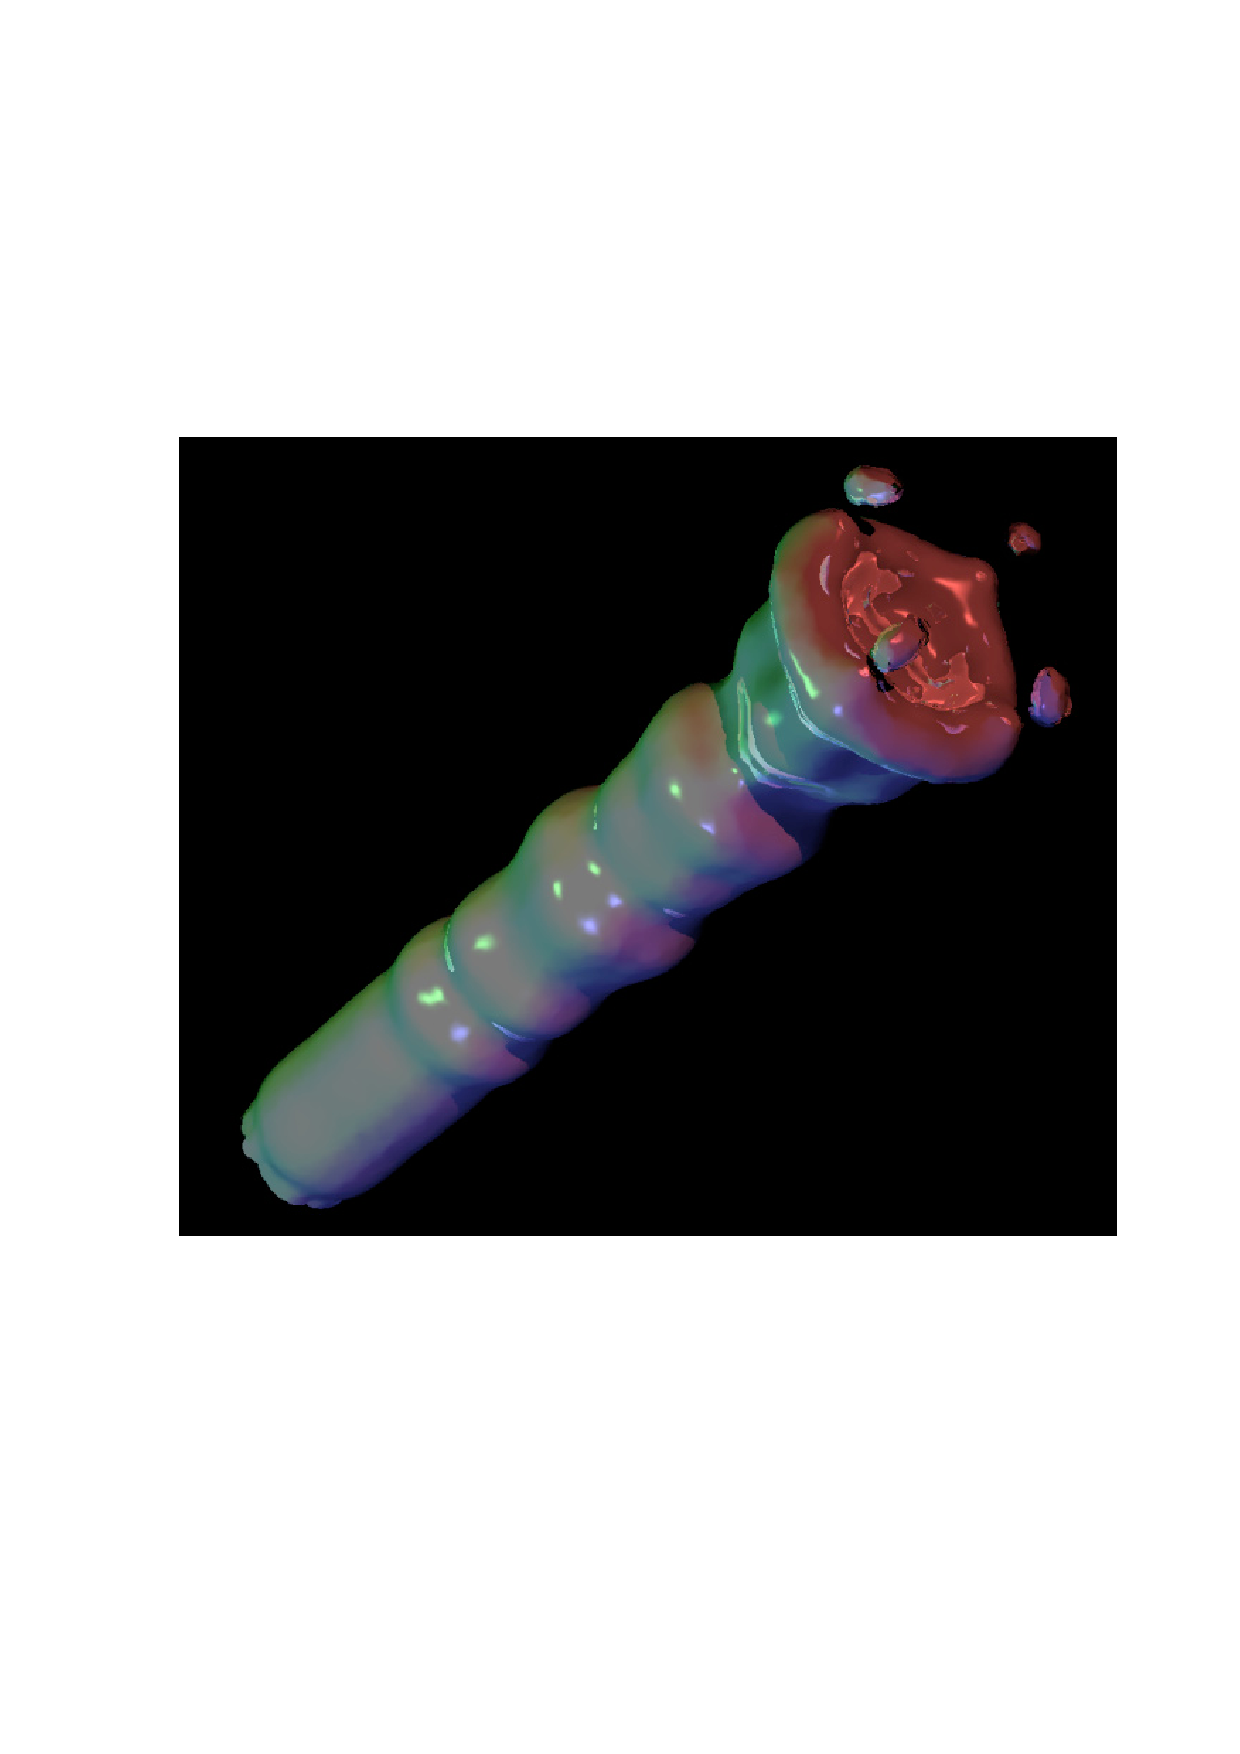
\includegraphics[width=\hsize]{Linsen_2006_Fig1.pdf}
    \caption{Point-based ray tracing of isosurface directly extracted from a scattered
      volume data. The scattered data set is a uniform random sampling of simulation data
      of fuel injection into a combustion chamber.}
    % \caption{Point-based ray tracing of isosurface directly extracted from a scattered
    %   volume data. The scattered data set is a uniform random sampling of simulation
    %   data of fuel injection into a combustion chamber.}
    % \label{fig:profxxx}
   \end{center}
\end{figure}

\noindent
{\em Using Ray Intersection for Dual Isosurfacing.}
Isosurface extraction using dual contouring approaches have been developed to generate a
surface that is dual in terms of the underlying extraction procedure used when compared to
the standard Marching Cubes (MC) method. These approaches address some shortcomings of the
MC methods including feature-detection within a cell and better triangles. We have
developed a simple method based on the MC method and the ray intersection technique to
compute isosurface points in the cell interior. One of the advantages of our method is
that it does not require Hermite data, i.e., the discrete scalar values at vertices
suffice. We compute ray intersections to determine isosurface points in the interior of
each cell, and then performed a complete analysis of all possible configurations to
generate a look-up table for all configurations.  We use a look-up table to optimize the
ray intersection method to obtain minimum number of points necessarily sufficient for
defining topologically correct isosurfaces in all possible configurations.

\noindent
{\em Structure-accentuating Dense Flow Visualization.}
Vector field visualization approaches can broadly be categorized into approaches that
directly visualize local or integrated flow and approaches that analyze the topological
structure and visualize extracted features. Our goal was to come up with a method that
falls into the first category, yet reveals structural information. We have developed a
dense flow visualization method that shows the overall flow behavior while accentuating
structural information without performing a topological analysis. A flow integration step
generates a density field by tracing particles under the influence of the underlying
vector field. The resulting density is high in attracting regions and low in repelling
regions. Density is measured by the number of particles per region accumulated over
time. The density fields for forward and backward propagation are explored using
texture-based rendering techniques.  We obtained dense flow visualizations that display
the overall flow behavior, emphasize critical and separating regions, and indicate flow
direction in the neighborhood of these regions.

\begin{figure}[ht]
  \begin{center}
     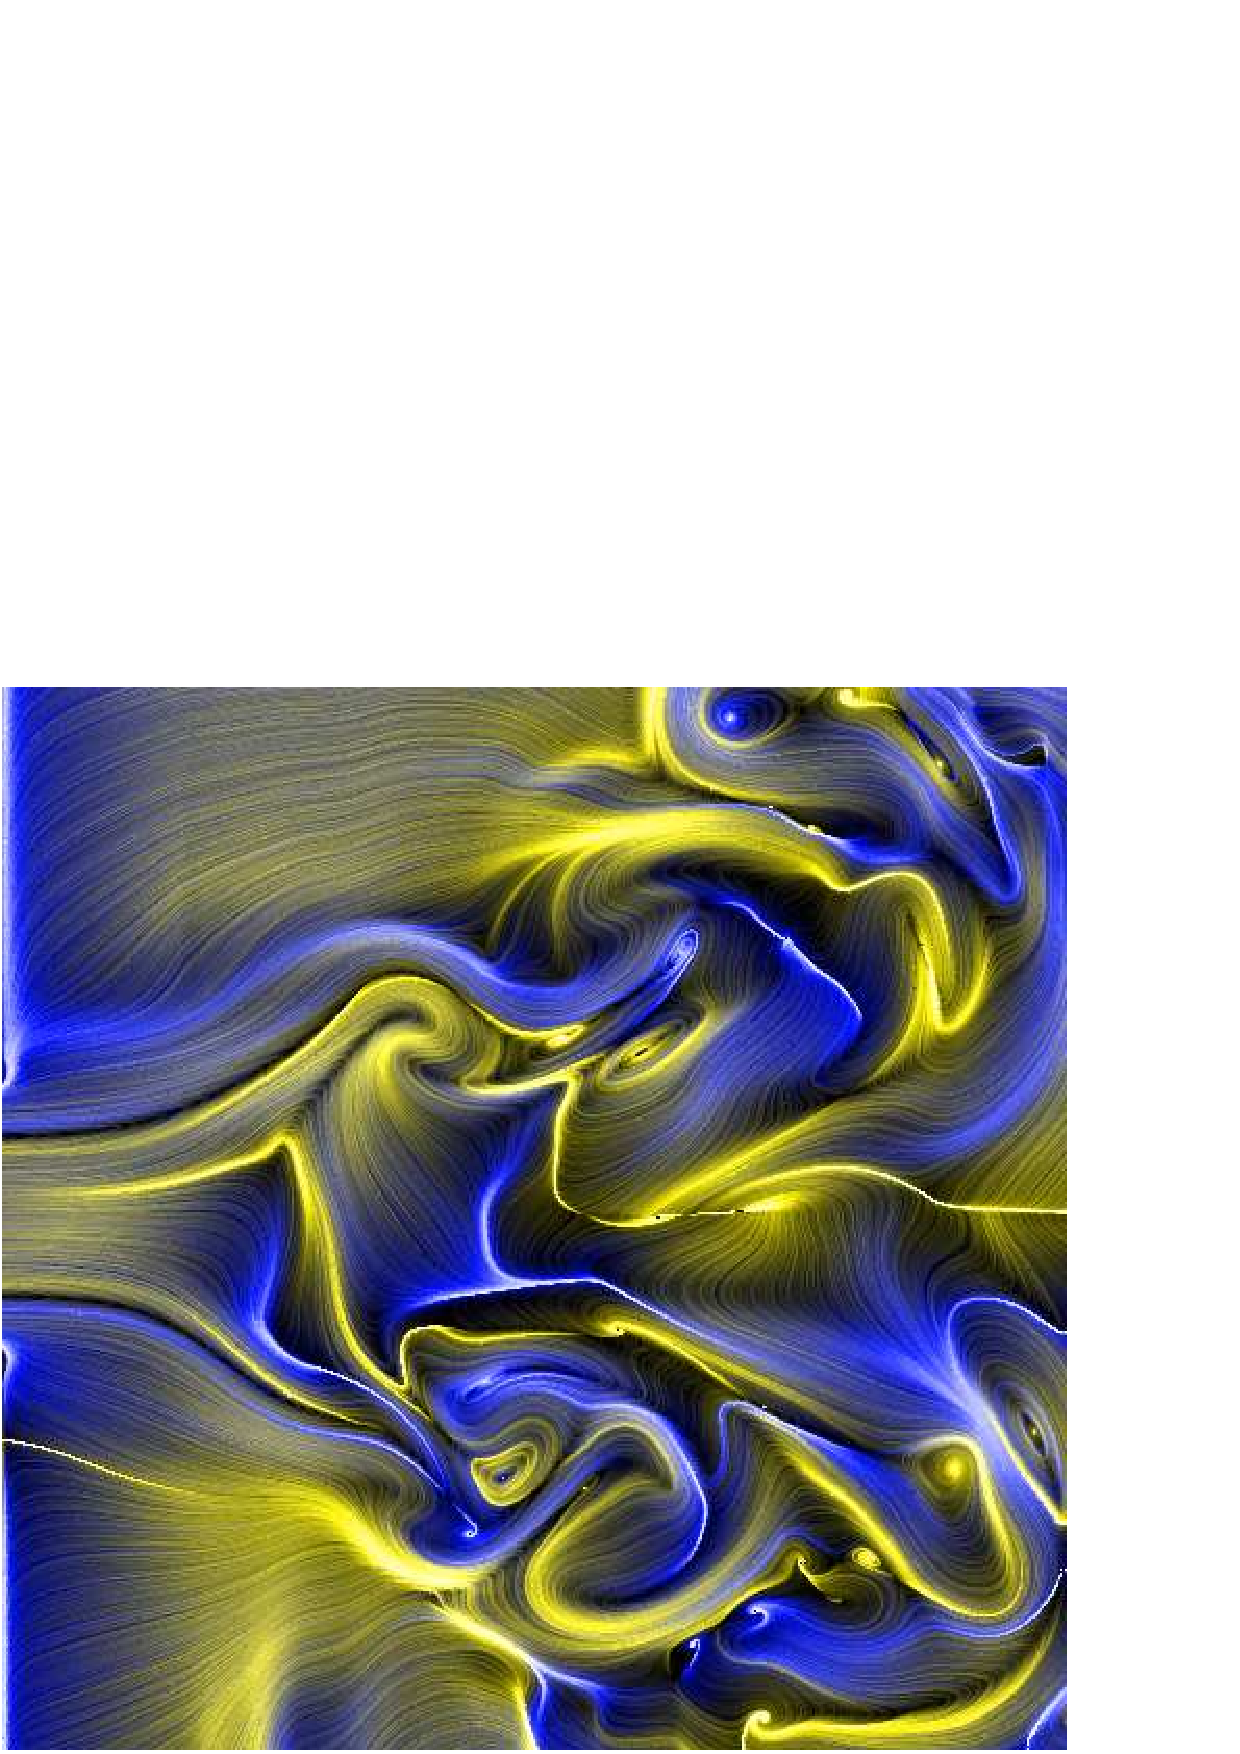
\includegraphics[width=\hsize]{Linsen_2006_Fig2.pdf}
    \caption{Structure-accentuating dense flow visualization applied to 2D simulation of
      a swirling jet.}
    %\caption{Structure-accentuating dense flow visualization applied to 2D simulation of a swirling jet.}
     % \label{fig:profxxx}
   \end{center}
\end{figure}

\noindent
{\em Visual Analysis of Gel-free Proteome Data.}
We developed a visual exploration system supporting protein analysis when using gel-free
data acquisition methods. The data to be analyzed is obtained by coupling liquid
chromatography (LC) with mass spectrometry (MS). LC-MS data has the properties of being
non-equidistantly distributed in the time dimension (measured by LC) and being scattered
in the mass-to-charge ratio dimension (measured by MS).  A hierarchical data
representation and visualization method is used for large LC-MS data. Based on this
visualization we have developed a tool that supports various data analysis steps like
deisotoping, landmark-based registration, and differential protein expression
analysis. Our visual tool provides a global understanding of the data, intuitive detection
and classification of experimental errors, and extensions to LC-MS/MS, LC/LC-MS, and
LC/LC-MS/MS data analysis.


\paragraph{Organization}
% list the (research) events you have organized, if any,

\begin{enumerate}
\item International conference on {\em Visualization in Medicine and Life Sciences (VMLS
    06)} held July 19--21, 2006, at Binz, R{\"u}gen, Germany
  (http://www.lars-linsen.de/vmls).  Organizers: Lars Linsen, Hans Hagen (University of
  Kaiserslautern), and Bernd Hamann (University of california, Davis).
\end{enumerate}

\paragraph{Collaborations}
\begin{enumerate}
\item {\sl Institut f{\"u}r Mathematik und Informatik, Ernst-Moritz-Arndt-Universit{\"a}t Greifswald, Germany}.\\
  Prof.~Georg F{\"u}llen, Julia L{\"o}cherbach, Steffen Rudnick.\\
  (1) Visualization of protein-protein interaction. \\
  (2) Visualization of gel-free proteomics data.\\
  (3) Simulation and animation of urban tree growth.
\item {\sl Institut f\"ur Mikrobiologie, Ernst-Moritz-Arndt-Universit\"at
    Greifswald, Germany}. \\
  Prof.~Michael Hecker, Dr.~J{\"o}rg Bernhardt, Dr.~D{\"o}rte Becher.\\
  Visualization of gel-free proteomics data.
\item {\sl Decodon GmbH, Greifswald, Germany}. \\
  Dr.~Matthias Berth, Dr.~J{\"o}rg Bernhardt.\\
  Visualization of gel-free proteomics data.
\item {\sl Institut f\"ur Diagnostische Radiologie und Neuroradiologie,
    Ernst-Moritz-Arndt-Universit\"at
    Greifswald, Germany}. \\
  Prof.~Norbert Hosten, Dr.~S{\"o}nke Langner, Martin Domin. \\
  Glyph- and tracking-based visualization of diffusion MRT data.
\item {\sl Poliklinik f\"ur zahn\"arztliche Prothetik und Werkstoffkunde,
    Ernst-Moritz-Arndt-Universit\"at
    Greifswald, Germany}. \\
  Prof.~Bernd Korda{\ss}.\\
  Virtual placement and interactive optimization for functional occlusion in
  prosthodontics.
\item {\sl Institut f\"ur Psychologie, Ernst-Moritz-Arndt-Universit\"at
    Greifswald, Germany}. \\
  Prof.~Klaus Landwehr.\\
  An interactive system for the generation of symmetric images with respct to symmetry
  groups.
\item {\sl Fraunhofer-Institut f\"ur Produktionstechnologie, Aachen, Germany}. \\
  Prof.~Christian Brecher, Prof.~Fritz Klocke, Lothar Glasmacher, Dr.~Olaf Dambon, Richard Zunke, Timo Wenzel.\\
  MoldFinish: Intelligent polishing system for automated finishing in tool and mold
  making.
  % (1) MoldFinish: Intelligents Poliersystem zur Automatisierung und Endbearbeitung im Werkzeug- und Formenbau.\\
  % (2) IProM: Multi-senorielle Messtechnik in Produktionsmaschinen
\item {\sl Institute for Data Analysis and Visualization (IDAV), University of California,
    Davis, U.S.A.} \\
  Prof.~Bernd Hamann, Prof.~Kenneth I.~Joy, Prof.~Nina Amenta, Prof.~John D.~Owens, Prof.~Oliver G.~Staadt, Dr.~Oliver Kreylos, Dr.~David F.~Wiley, Sung Park, Jaya Sreevalsan-Nair. \\
  (1) New approaches in flow visualization.\\
  (2) Exact dual isosurface extraction.\\
  (3) Interactive visual exploration of Northern California's water monitoring network.\\
  (4) Surface-based brain morphing.
\item {\sl Zuse Institut Berlin, Germany.}\\
  Prof.~Ingrid Hotz.\\
  (1) New approaches in flow visualization.\\
  (2) Interactive visual exploration of Northern California's water monitoring network.
\item {\sl Center for Urban Forest Research, University of California,
    Davis, U.S.A.} \\
  Prof.~E.~Gregory McPherson. \\
  Simulation and animation of urban tree growth.
\item {\sl Center for Functional MRI, Department of Radiology Department, University of California,  San Diego, U.S.A.} \\
  Prof.~Lawrence R.~Frank, German Eichberger.\\
  Automated segmentation of anatomical scans (MRT) of sharks.
  % \item {\sl Center for Neuroscience, University of California, Davis, U.S.A.} \\
  %   (Edward G.~Jones, Bruno A.~Olshausen).
  % \item {\sl Department of Mechanical and Aeronautical Engineering, University of
  %     California, Davis, U.S.A.} \\ (Anthony S.~Wexler).
\end{enumerate}


\paragraph{Grants}
% list the running grants in 2006, if none have been received, please delete this
% subsection.
\begin{enumerate}
\item DFG supported the International conference on Visualization in Medicine and Life
  Sciences (VMLS 06).
\end{enumerate}


%\paragraph{Awards, Prizes}
% list the awards you have received in 2006, if none have been received, please delete this
% subsection.
%\begin{enumerate}
%\item
%\item
%\end{enumerate}

%Publications should be delivered as a separate file (naming
%convention profxxx.bib. See description by R. Helling. Please make
%sure that all your publications are referred to in the TiX file.
%This can either be in form of a \cite{profxxxkey} or as a
%\nocite{profxxxkey} in the end. A publication which is not
%referred to on the LaTeX file doesn't produce any output in the
%report.

\nocite{SreevalsanNairVanNiewenhuyseHotzLinsenHamann07}
\nocite{LinsenLoecherbachBerthBernhardtBecher06}
\nocite{ParkLinsenKreylosOwensHamann06}
\nocite{RosenthalLinsen06}
\nocite{ParkYuHotzLinsenHamann06}
\nocite{SreevalsanNairLinsenHamann06}
\nocite{VivodtzevWileyLinsenJonesAmentaHamannJoy06}
\nocite{EichbergerPerryWakerHastingsLinsenFrank06}
\nocite{LinsenHamannJoy06}

%\end{document}

%%% Local Variables:
%%% mode: latex
%%% TeX-master: report
%%% End:

  \putbib[combined]
\end{bibunit}
\begin{bibunit}[hplain]
  \subsubsection{Open Access Publishing}
\label{ict:stamer}
\index{Stamerjohanns, Heinrich}

\paragraph{Research Team}
Heinrich Stamerjohanns (Head of CS Labs), also member of KWARC
Research Team, see~\ref{ict:modeling:kohlhase}.\\

With the fundamental change of the existing paper publication system
towards networked digital publications a variety of new possibilities arise
to overcome the existing technical constraints of scientific documents
in order to increase the effectiveness of scientific research.

Scientific exchange may be improved in various ways:
\begin{myitemize}
\item by giving free and and unrestricted access (Open Access) to
the results of scientific research
\item by enabling access not only to text and pixeled images
but to complete sources (data, programs) of the obtained results
\item by semantically annotating content in order to improve
the searchability by machines.
\end{myitemize}

\paragraph{Highlights}

We proposed a content markup language for physics realized by
extending the OMDoc format by an infrastructure for the principal
concepts of physics: observables, physical systems, and experiments.
The formalization of the description of physics observables follows
the structural essence of the operational theory of physics
measurements. The representational infrastructure for systems and
experiments allow to capture the distinctive practice of physics:
natural laws are supported by evidence from experiments which are
described, disseminated and reproduced by others.

In a collaboration with Prof. Jeltsch we are also developing tools
to dynamically publish generated data that will help to understand the genetic
and epigenetic basis for DNA-methylation variation in the human genome,
to asses sequence specificity of DNA-methylation patterns in normal tissues.

\begin{figure}[ht]
  \begin{center}
    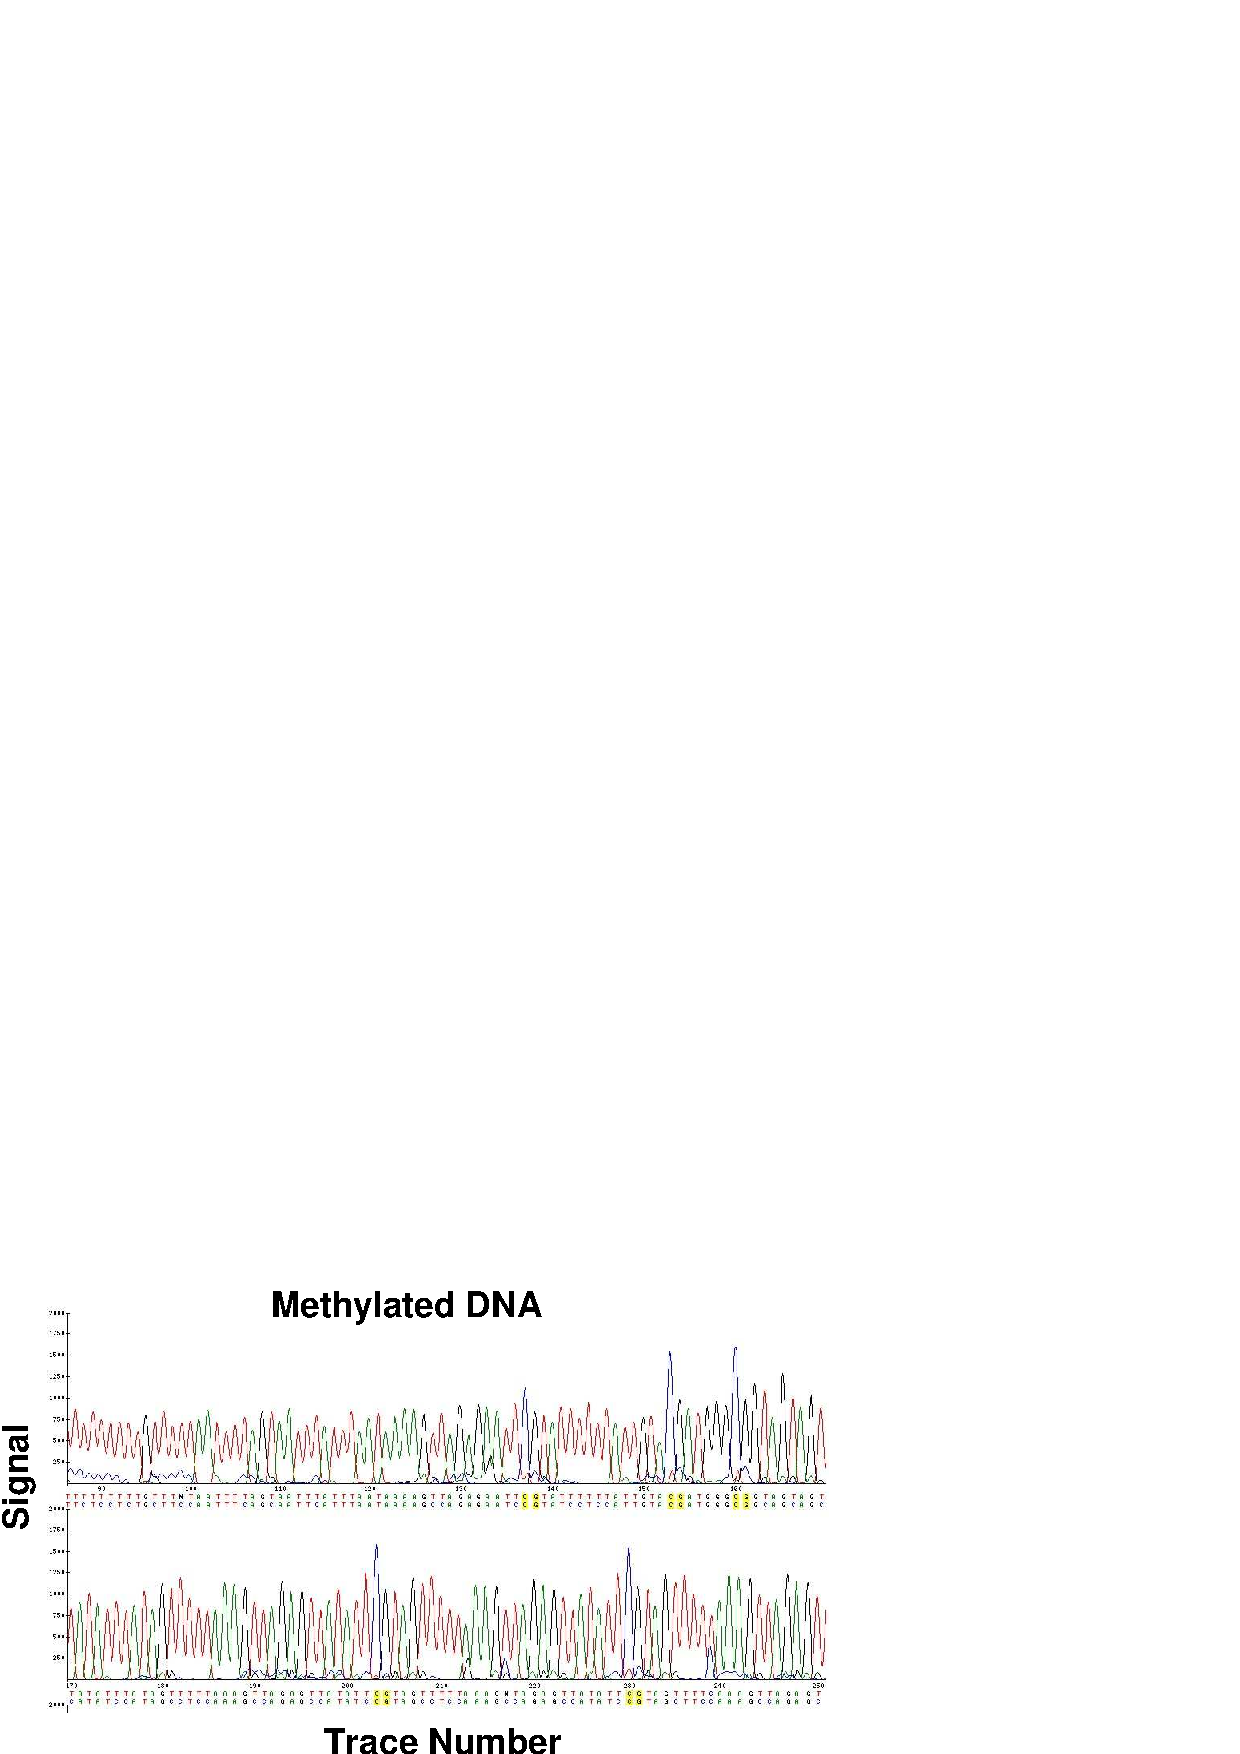
\includegraphics[width=\hsize,bb=0 0 390 230]{stamerjohanns-fig1.pdf}
    \caption{Dynamically created content of the analysis of methylated DNA. Other
    researches do not only have access to images, but to full research data.}\label{fig:stammerjohanns}
   \end{center}
\end{figure}

As a member of the Deutsche Initiative f\"ur Netzwerkinformation (DINI)
Working Groups \textsl{E-Publications}
and \textsl{Open Archives}, we are trying to establish common standards
for Scientific Institutional Repositories.

\paragraph{Collaborations}
\begin{enumerate}
    \item {\sl International University  Bremen} \\
            Prof. M. Kohlhase \\
            Extending OMDOC to PhysML, ArXiv conversion     \\
            Prof. A. Jeltsch \\
            Dynamic publishing of SMP Epigenetics Data

    \item {\sl ISN Oldenburg} \\
            Prof. E.R. Hilf \\
            Extending OMDOC to PhysML\\
            Citation Linking and Indexing

    \item {\sl DINI Working Groups} \\
            Certificate for Institutional Repositories

\end{enumerate}

%\paragraph{Publications}
\nocite{HilKohSta:copmem06,DINI06}

  \putbib[combined]
\end{bibunit}
\begin{bibunit}[hplain]
  
\subsubsection{Networks and
Distributed Systems}\label{ict:cns:schoenwaelder} \index{Sch\"onw\"alder,
J\"urgen}

\paragraph{Research Team}
J\"urgen Sch\"onw\"alder (Professor), Ha Manh Tran (PhD Student), Vlad Balan (MSc
Student), Mat\'u\v{s} Harvan (MSc Student), Vladislav Marinov (MSc Student)\\

Computer networks such as the Internet continue to change many aspects
of our daily life. The networks and protocols research group carries
out research related to Internet protocols, with strong relationships
to work undertaken by the Internet Engineering Task Force (IETF), an
organization responsible for Internet protocol standardization, and
the Internet Research Task Force (IRTF), an organization responsible
for longer-term research related to Internet protocols.

\paragraph{Highlights}

The operation of increasingly complex communication networks requires
supporting systems, so called network management systems.  Network
management protocols and associated data definitions have been
developed and standardized over the last decade to support open,
vendor-neutral access to management and control information.  While
some of these technologies are in wide-spread usage, there is little
information how the underlying protocols are utilized and what the
specific characteristics of network management interactions are. As a
consequence, there are no well accepted models which can be used to
analyze the impact of protocol changes.

\begin{figure}[ht]
  \begin{center}
     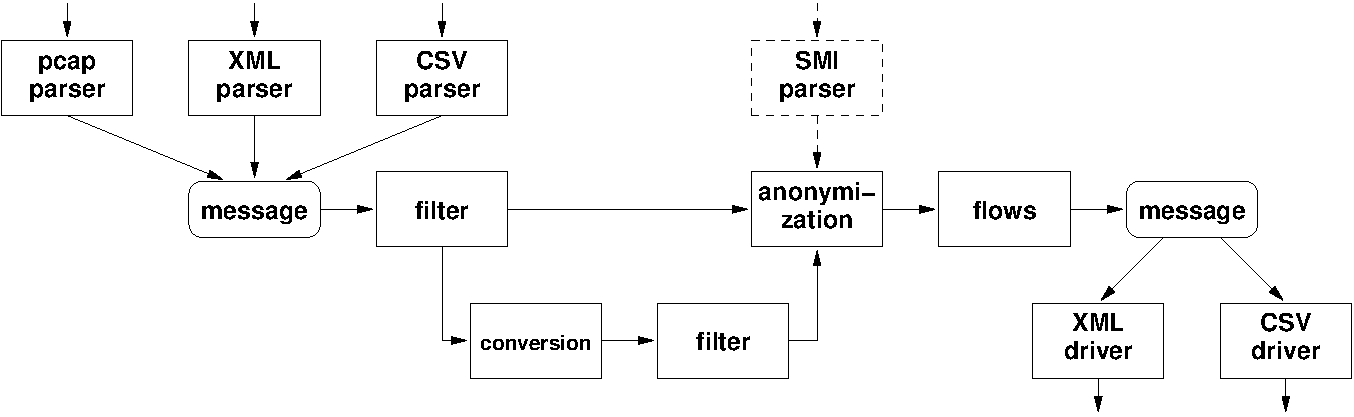
\includegraphics[width=\hsize]{schoenwaelder-tools}
  \end{center}
  \caption{Data flow within the \texttt{snmpdump} tool}\label{fig:snmpdump}
\end{figure}

A larger empirical study has been started in 2006 where we collect network management
packet traces from operational networks. This study is carried out in collaboration with
international research groups and supporting operators in order to obtain traces from live
networks. Based on an anonymization algorithm developed in 2005 \cite{HS06}, our group has
designed and implemented a tool chain (Fig.~\ref{fig:snmpdump}) for the analysis of
network management traffic traces \cite{PSHSM07}. Further research is ongoing to develop
analysis algorithms able to infer high-level management operations from observed primitive
protocol operations.

\begin{figure}[ht]
  \begin{center}
     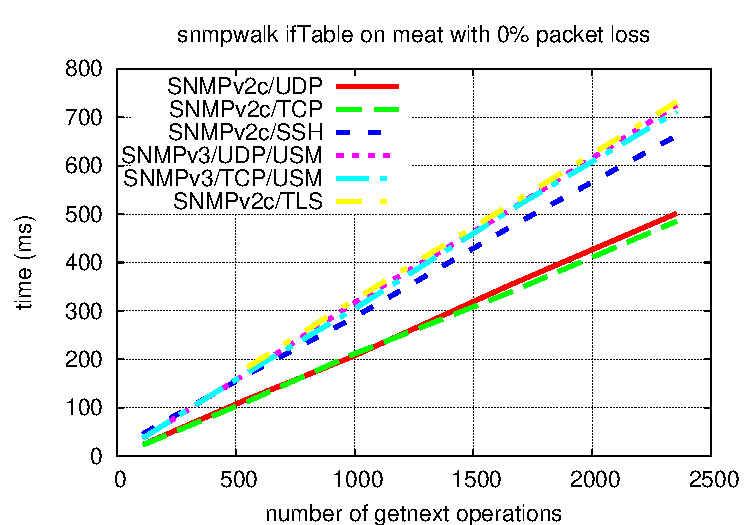
\includegraphics[width=\hsize]{schoenwaelder-sec}
  \end{center}
  \caption{Latency of SNMP/SSH and SNMP/TLS}\label{fig:sshtls}
\end{figure}

A related activity concerns the security of network management
interactions (Fig.~\ref{fig:sshtls}). We have prototyped and analyzed
a security extension proposed for the SNMP which leverages transport
layer security protocols such as SSH or TLS \cite{MS06}. This work is
related to standardization efforts undertaken by the Integrated
Security Model for SNMP (ISMS) working group of the IETF.

\begin{figure}[ht]
  \begin{center}
     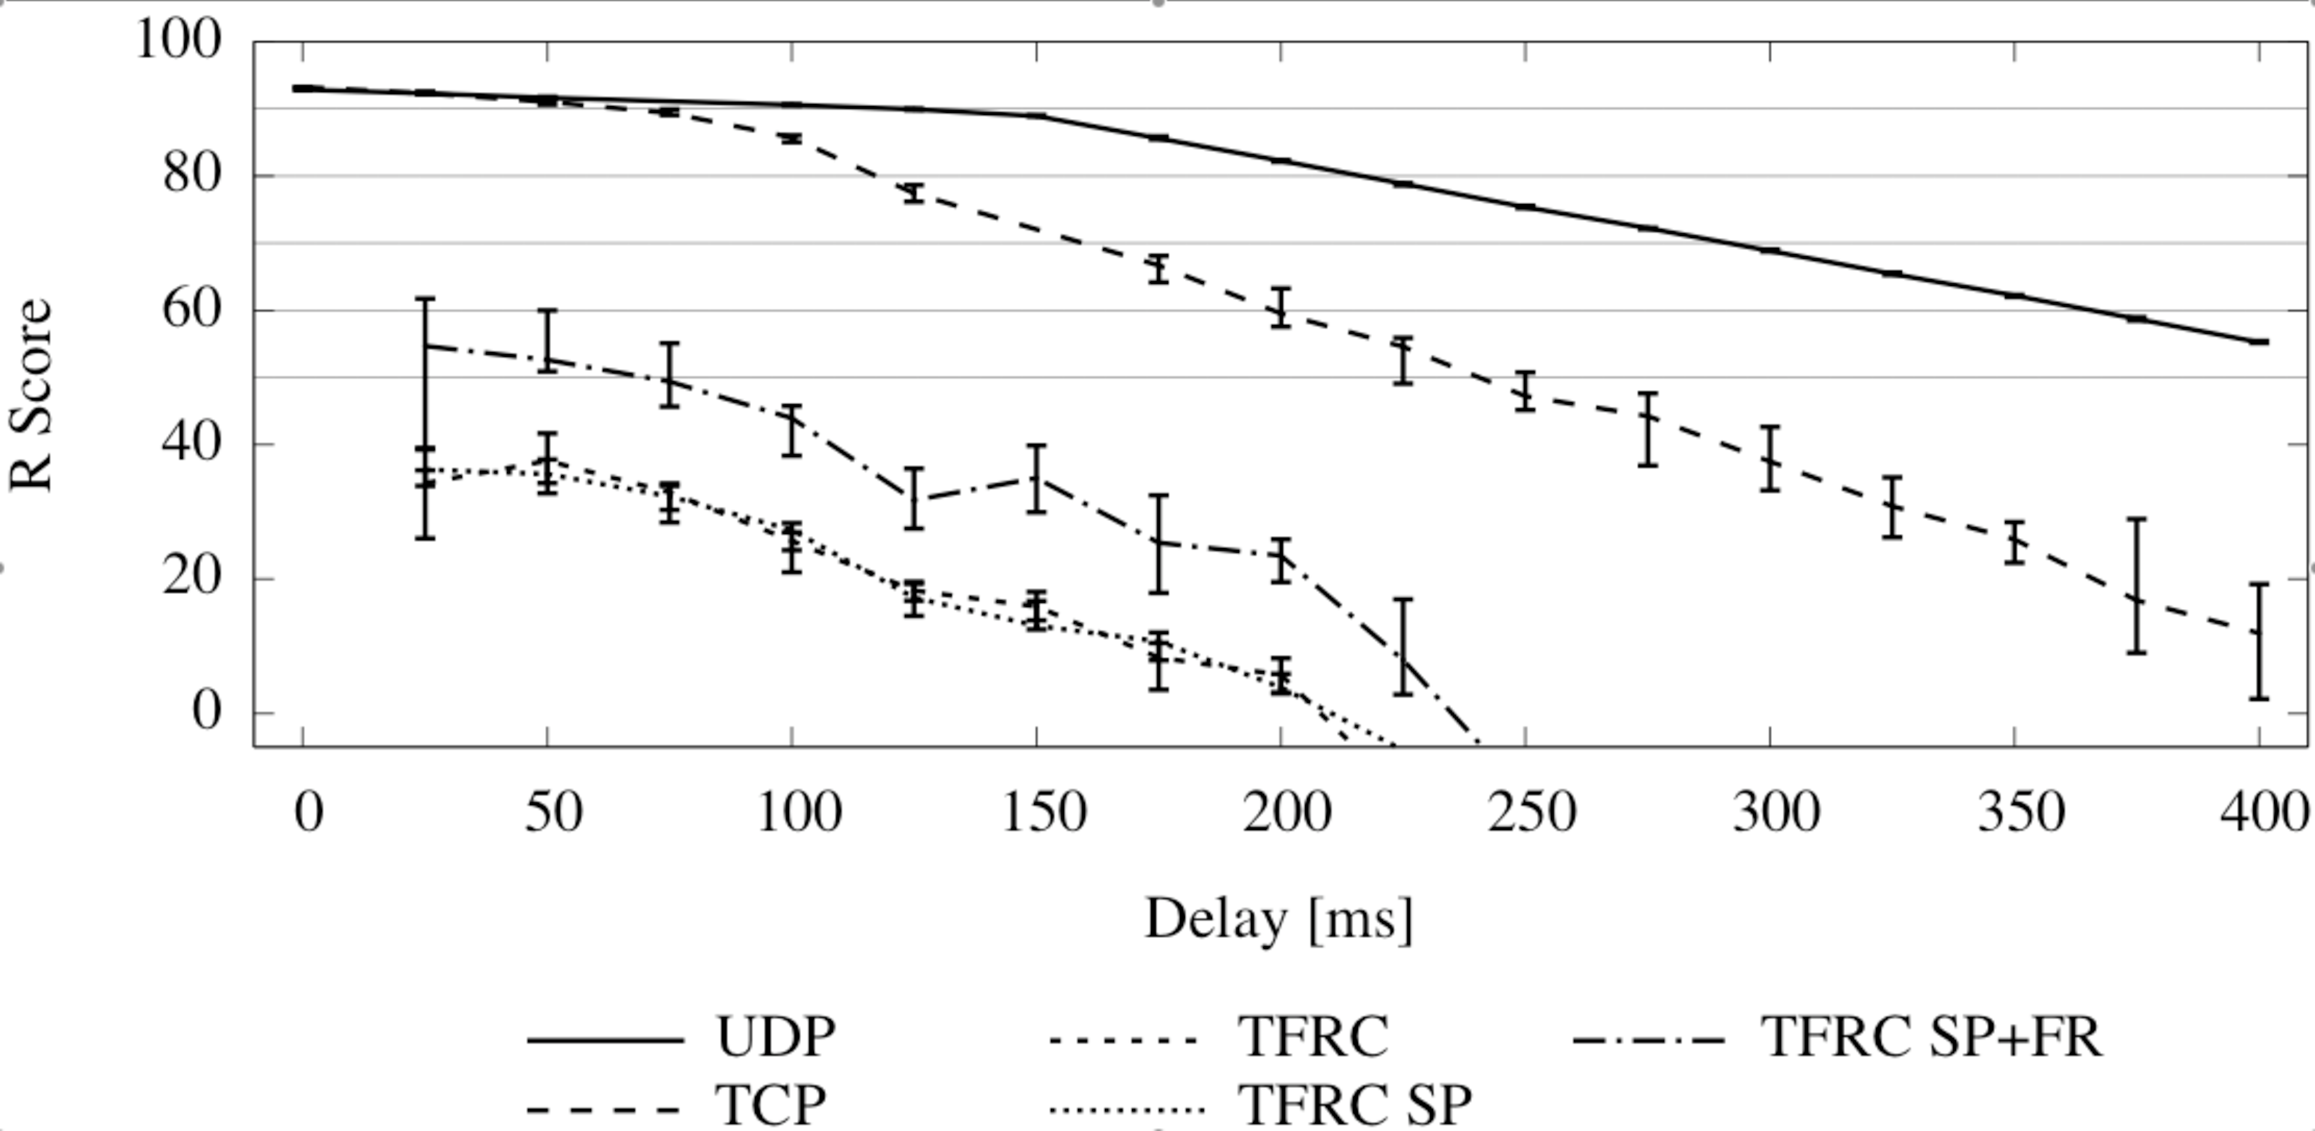
\includegraphics[width=\hsize]{schoenwaelder-dccp}
  \end{center}
  \caption{R scores for G.711 over DCCP}\label{fig:sshtls2}
\end{figure}

Finally, we have conducted research on the performance of voice stream
transmission over the new Data Congestion Control Protocol (DCCP)
being standardized by the IETF \cite{BENB07}. This work was carried out in
close collaboration with NEC C\&C Research in Heidelberg, Germany.


\penalty -50
\paragraph{Organization}\nobreak
% list the (research) events you have organized, if any,
\begin{enumerate}
    \item Editorial board member of the IEEE electronic Transactions on
          Network and Service Management
    \item Guest Co-Editor of a special issue on Peer-to-Peer
          Technologies in Network and Service Management of the
          Journal of Network and Systems Management
    \item Program Committee member of NOMS 2006, ACC 2006, DSOM 2006,
          IM 2007, ICCC 2007 NSO, SASO 2007, AIMS 2007
    \item Reviewer IEEE Communications Magazine, IEEE Transactions on
          Software Engineering, Springer Journal of Network and
      Systems Management
    \item Co-Chair of the IETF ISMS working group
    \item Member of the Security Directorate of the IETF
    \item Chair of the Network Management Research Group (NMRG) of the IRTF
    \item Chair of the 19th NMRG workshop on ``Promise Theory and New
          Approaches to Distributed Management'', KTH, Stockholm, January
          2006
    \item Chair of the 21st IRTF NMRG workshop on ``Future Direction
          of Network and Service Management Research'', SurfNet,
          Utrecht, October 2006
    \item Dissemination Activity Leader / Member of the Executive
          Committee of the EMANICS Network of Excellence
\end{enumerate}

\paragraph{Collaborations}
\begin{enumerate}
    \item {\sl University of Twente, The Netherlands}\\
          Prof.\ Aiko Pras\\
          Network Management, Traffic Measurements
    \item {\sl INRIA Lorraine, France}\\
          Prof.\ Olivier Festor\\
          Scalability of Management Protocols
    \item {\sl NEC C\&C Research}\\
          Dr.\ Lars Eggert\\
          Analysis of Voice over the Datagram Congestion Control Protocol
    \item {\sl NEC C\&C Research}\\
          Dr.\ J\"urgen Quittek\\
          Integrated Security Model for the Simple Network Management Protocol (SNMP)
    \item {\sl Huawei}\\
          David Harrington\\
          Architectural Models for Internet Management Protocols
    \item {\sl IEEE Project 802}\\
          Tony Jeffree\\
          SNMP over IEEE 802 Networks
\end{enumerate}

\paragraph{Grants}
\begin{enumerate}
    \item Funded by EU-IST NoE,  \emph{ ``EMANICS (EU Network of Excellence for the Management
      of Internet Technologies and Complex Services)''}, (January 2006 - December
      2009)
\end{enumerate}

%\paragraph{Awards, Prices}
%\begin{enumerate}
%\item IM 2005 Distinguished Experts Panel (invited panelist)
%\end{enumerate}

%\paragraph{Publications}

%\begin{description}
%  \item[Conference Proceedings]
  \nocite{HS06} \nocite{MS06} \nocite{BENB07}
  \nocite{PSHSM07} \nocite{DKPM07}
  %\item[Books/Collections]
  \nocite{Sch07}
 % \item[Standards]
  \nocite{RFC4789}
%\end{description}
%\end{document}
%%% Local Variables:
%%% mode: latex
%%% TeX-master: "report"
%%% End:

  \putbib[combined]
\end{bibunit}
\begin{bibunit}[hplain]
  \subsubsection{Machine Learning}
\index{Jaeger, Herbert}
\paragraph{Research Team}
Herbert Jaeger (Professor), Mingjie Zhao (Postdoctoral Fellow), Mantas Lukosevicius (PhD student)\\


Herbert Jaeger and his team develops Machine Learning methods for
the automated construction of prediction models from empirical
time series data.  Target applications (and collaborations) are in
the fields of neurobiology, human music understanding, handwriting
recognition, control engineering and telecommunication. Two main
methods investigated in Herbert Jaeger's group are recurrent
neural networks of the ``Echo State Network'' (ESN) type and
observable operator models (OOMs). ESNs are interesting not only
because they yield highly efficient learning algorithms but also
because they offer a biologically plausible model of learning in
natural brains. OOMs generalize hidden Markov models, a standard
tool in speech and text recognition, yielding more expressive
models in a fraction of the learning time required for hidden
Markov models. Both ESNs and OOMs have been originally found by
Herbert Jaeger and have been investigated in his group over the
last few years.



\paragraph{Highlights}

An important application of machine learning methods for time series
data is speech recognition. Almost all current methods in this field
rely on ``hidden Markov models'' as the basic machine learning
technique. Although recurrent neural networks (RNNs) would be more
plausible from a bionics perspective -- after all, our brains are RNNs
--, and although it is known that artificial RNNs can, in principle,
yield optimal speech signal decoders, these models have not in
practice been used due to the extreme computational cost and the
danger of instability of previously known training methods for RNNs.
RNNs of the Echo State Network type are computationally cheap to train
and intrinsically stable. Thus, one research direction in Jaeger's
group is to tailor ESNs to speech processing tasks.

A widely used benchmark task in this field is the ``Japanese Vowels''
problem\footnote{Data donated by Mineichi Kudo, Jun Toyama, and Masaru
  Shimbo; obtainable at \url{http://kdd.ics.uci.edu}}. The training
data consist of pre-processed vocal recordings from 9 Japanese
speakers, with 30 recordings per speaker. The task is to train from
these data a classificator that can recognize the speaker in test
recordings. Figure \ref{fig:JaegerFig1} shows some recordings from the
training set. The task is difficult because of high intra-speaker
 and low inter-speaker  variability. The best known classification
 methods achieve a test error rate of slightly less than 2 \%. Using
 ESN-based models with an unconventional architecture (combining the
 classification ``votes'' of 1,000 tiny ESNs with a particular neuron
 model which is more biologically plausible than standard artificial
 neuron models), Jaeger et al.\ achieved a \emph{zero} test error
 \cite{Jaegeretal2}.

\begin{figure}[ht]
  \begin{center}
   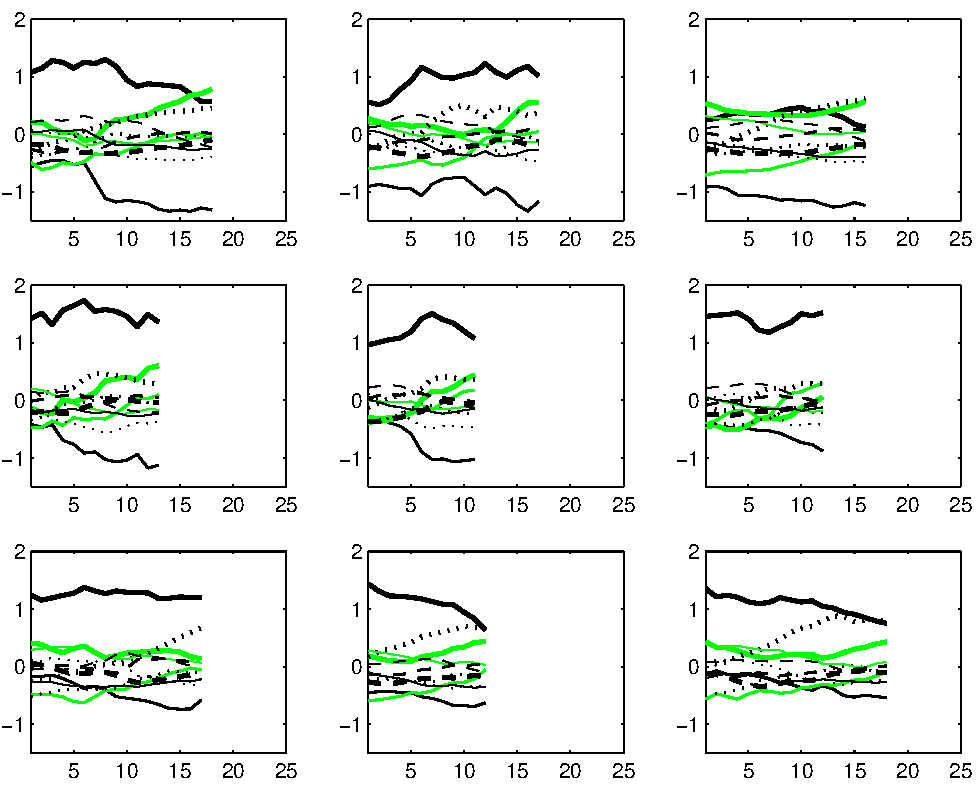
\includegraphics[width=\hsize]{JaegerFig1_2006.pdf}
    \caption{Some samples from the ``Japanese Vowels'' benchmark dataset. Each
    row shows three recordings from one speaker.}\label{fig:JaegerFig1}
   \end{center}
\end{figure}

Another important application of machine learning methods for time
series data is the recognition of handwritten texts. This task occurs,
for instance, in automated check reading systems or automated mail or
parcel sorting facilities. The text that is to be recognized is read
from left to right with a video reading head, yielding a video
sequence much like the visual input used by humans who read a text.
One difficulty in this domain arises from the circumstance that
handwritings can be narrow or stretched -- and this may even change
within a single written text. This is known as ``time warping''. An
automated reading system must be able to accomodate itself online to
changing character widths -- it must ``read faster'' when the
characters are narrow and ``read slower'' when they are
stretched. This poses a nasty chicken-and-egg problem: accomodation
would be easy if the characters were already recognized, but in order
to recognize them, the reading system must first accomodate to the
local ``writing speed''. Today's standard approach is to use dynamic
programming methods to optimize the local ``reading speed''. These
methods are computationally expensive and again, not biologically
plausible.

In a collaboration with Planet AG (Schwerin), a company specializing
in text recognition systems, a new ESN design was developed which
achieves an online accomodation to ``writing speed'' with no
additional computational cost, neither in the training phase nor in
the exploitation phase. So far, this
method was tested on synthetic data only, where it achieved a
close-to-optimal recognition performance \cite{Jaegeretal1,
  Jaegeretal2}. The collaboration with Planet AG will continue through
2007 and beyond.



\paragraph{Organization}
% list the (research) events you have organized, if any,

\begin{enumerate}
\item Interdisciplinary College 2006, G\"unne, Germany (member of program committee)
\item Studienstiftung Summer Academy Alpach 2006, Course ``Neuronal Plasticity'' (with D.\
  Jaeger, Emory University)
\item Special issue of \emph{Neural Networks} on ESNs and ``Liquid State Machines'', guest
  co-editor
\item ESN and ``Liquid State Machine'' workshop at NIPS 2006 (co-organizer)
\item Coordinator of a joint IUB -- University Bremen \emph{Exzellenzinitiative} proposal
  ``Bremen Graduate School for Computational Modeling of Complex Systems''
\end{enumerate}

\paragraph{Collaborations}
\begin{enumerate}
\item {\sl TU Graz} \\ Prof. Wolfgang Maass \\ Echo State Networks and Liquid State
  Machines
\item {\sl Planet AG, Schwerin} \\ Echo State Networks for handwriting recognition
\item {\sl Emory University, Atlanta} \\ Prof. Dieter Jaeger \\
  Biological and artificial models of neuronal plasticity
\item {\sl Universit\'e de Montr\'al} \\ Prof. Douglas Eck \\ Echo State Networks for
  music processing
\item {\sl Fraunhofer Institute IAIS, Sankt Augustin} \\ Prof. Paul
  Pl\"oger \\ ESNs for robot control
\item {\sl Universit�t K\"oln}\\ Dr. Alexander Sch\"onhuth \\ Mathematical theory of
  observable operator models
\end{enumerate}


\paragraph{Grants}
% list the running grants in 2005, if none have been received, please delete this
% subsection.
\begin{enumerate}
\item Funded by DFG, \emph {Quadratic observable operator models},
(December 2005 - December 2007)

\item Funded by private partner Planet AG, Schwerin,
\emph{Time-warping invariant echo
  state networks}, (September 2005 - August 2006)
\end{enumerate}

\nocite{Jaeger3}

%%% Local Variables:
%%% mode: latex
%%% TeX-master: "report"
%%% End:

  \putbib[combined]
\end{bibunit}
\begin{bibunit}[hplain]
  \subsubsection{Robotics}\label{ict:robotics:birk}
\index{Birk, Andreas}

\paragraph{Research Team}
Andreas Birk (Professor),
Kaustubh Pathak (Postdoctoral Fellow),
Winai Chonnaparamutt (PhD Student),
Mohammed Nour Abdel-Gwad Ahmed (PhD Student),
Max Pfingsthorn (PhD Student),
Jann Poppinga (PhD Student),
S\"{o}ren Schwertfeger (PhD Student) \\

The research of the Birk group focuses on Autonomous Systems. The work ranges from the
development of embedded hardware via mechatronics and sensors to high-level software. On
the basic research side of autonomous systems, machine learning and cooperation are core
activities. The robotics systems developed are used in various domains including
underwater and especially rescue robots.

 Especially mobile robots can be highly valuable tools in urban rescue
missions after catastrophes like earthquakes, bomb- or gas-explosions or daily incidents
like fires and road accidents involving hazardous materials. The robots are used to
inspect collapsed structures, to assess the situation and to search and locate
victims. There are many engineering and scientific challenges. Rescue robots not only have
to be designed for the harsh environmental conditions of disasters, but they also need
advanced capabilities like intelligent behaviors to free them from constant supervision by
operators.  IUB robotics is among the world-wide leading groups in this domain.

\paragraph{Highlights}

The IUB rescue robots demonstrated their capabilities on several
occasions including technology demonstrations, especially the Rescue
Robot Field Test Demo (figure~\ref{fig:outdoor}) and the European
Land Robotics Trials (ELROB). The robots also demonstrated their
capabilities at several competitions, namely three RoboCup events.
At the RoboCup US Open in Atlanta, the IUB team won the first place
in the rescue robot league, beating the favored US American groups.
The team also won the first place at the European RoboCup
competition, the Dutch Open in Eindhoven. The team also got the
Innovation Award at the RoboCup World Championship in Bremen for
demonstrating for the first time the successful combined usage of a
tele-operated with a fully autonomous robot at rescue missions. IUB
was the only European team that made it to the final round at the
RoboCup World Championship, and it was beaten in the end by Asian
teams that purely relied on tele-operated devices without any
on-board intelligence.



\begin{figure}[thpb]
  \centering
  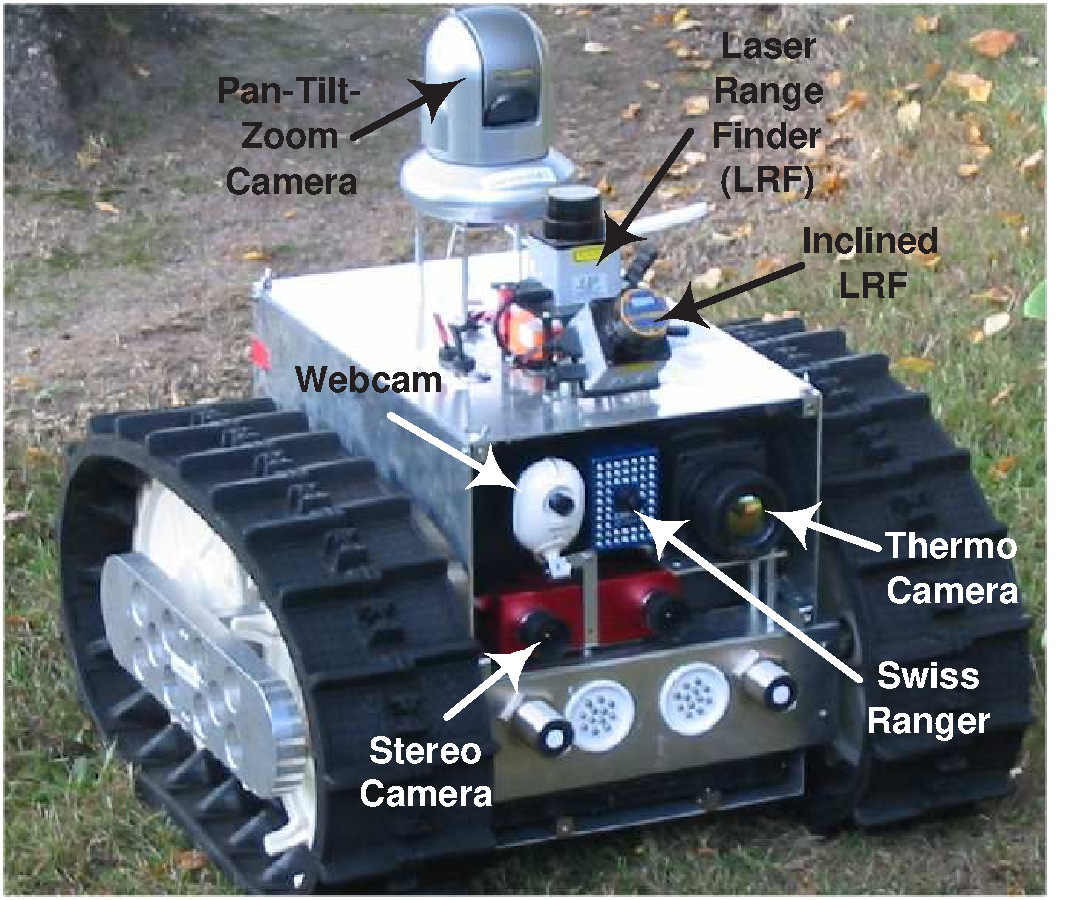
\includegraphics[width=\linewidth]{autonomousrobot.pdf}
  \caption{A {rugbot} with a selection of on-board sensors. Several sensors are dedicated
    to 3D range sensing to generate 3D environment models with a novel approach.}
  \label{fig:rugbot}
\end{figure}




On the research side, several contributions have been made ranging from the robot
mechatronics over on-board intelligence up to cooperative systems level.  Regarding the
mechatronics of the robots, a new locomotion system \cite{birk_flipper_rcup06} and a
special mobile communication system were developed \cite{birk_rescuecabledrum_rcup05}. The
latest type of robot from IUB robotics, the so-called rugbot, short for rugged robot, is
meanwhile one of the most advanced systems in this field \cite{birk_rugbot_ssrr06}. But
this holds not only for its mechatronic side but especially also with respect to its
on-board intelligence going up to full autonomy
\cite{birk_rescueteam_rcup05}. Contributions to several core topics for intelligent mobile
robot have been made in this context, especially for map generation
\cite{birkRescRobARJ06}, for the vectorization of maps
\cite{birk_mapvectorization_rcup06}, for the integration of autonomous behaviors with user
interactions \cite{birk_rescueGUI_rcup05}, and for the underlying architecture for
autonomy \cite{birk_autonomy_ssrr06}. The group also contributed to a high fidelity
simulator for mobile robots \cite{birk_virtualrobot_rcup05} that plays a significant role
in the prototype development of intelligent robot software.  Last but not least, work
regarding cooperative robot teams was done. The contributions include a novel algorithm
for multi robot exploration \cite{birk_CommExpore_CEP06} that can be used for search and
rescue missions by robot packs \cite{birk_commexplore_rcup05}. A second important result
is a novel algorithm for multi robot mapping \cite{BirkMultiMap_IEEEproc}.


\begin{figure*}
\centering
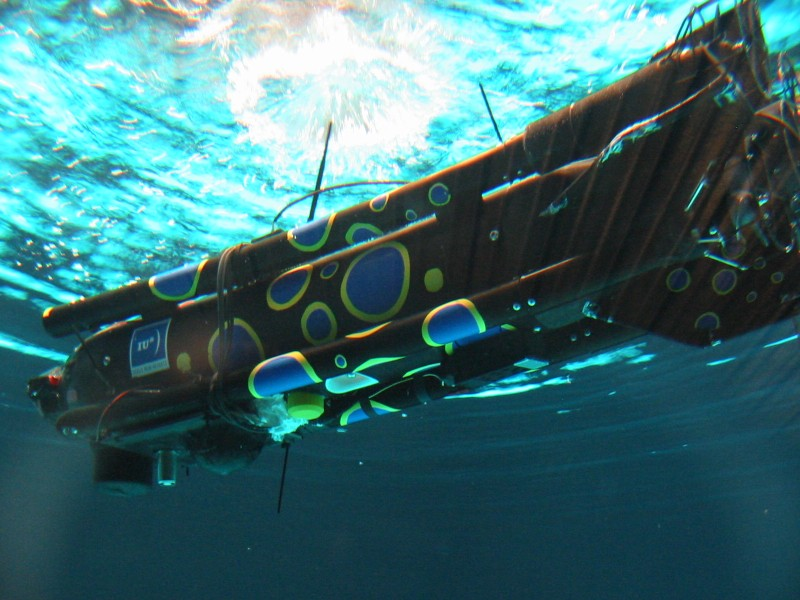
\includegraphics[width=.32\linewidth]{AUV-2006-best01.png}
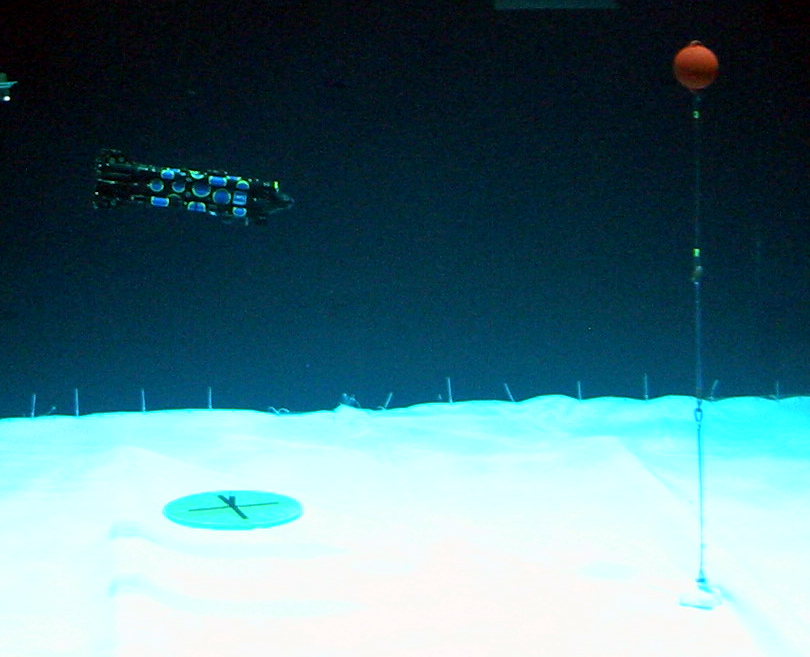
\includegraphics[width=.32\linewidth]{AUV-2006-best03.png}
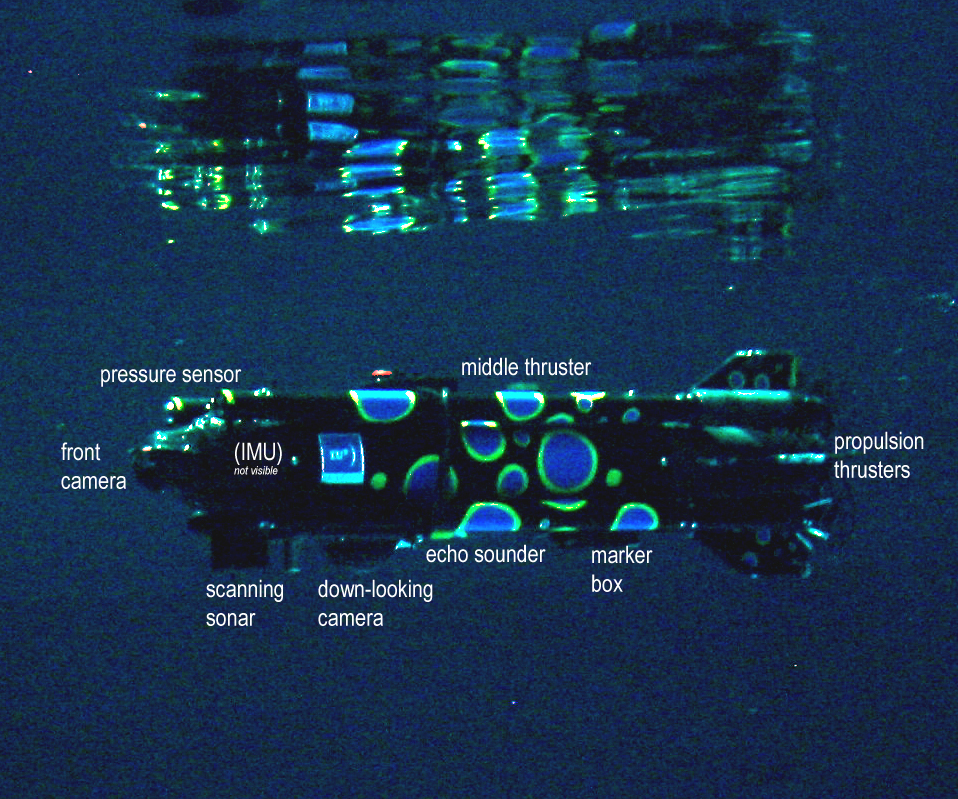
\includegraphics[width=.32\linewidth]{AUV-2006-best02-text.png}
\caption{The IUB-ATLAS Autonomous Underwater Vehicle (AUV) diving in a test pool
  (left). The AUV on an autonomous mission, searching for a midwater target in form of a
  submerged orange buoy (center). An overview of the main sensors of the AUV (right).}
\label{IUB-AUV}
\end{figure*}

IUB robotics made in 2006 also first successful practical steps in the domain of
underwater robotics by developing an Autonomous Underwater Vehicle (AUV). The work was
jointly done with ATLAS Elektronik in a cooperative project including also the IUB
robotics club. The most basic vehicle parts, namely the hull, the batteries, the motors
with propellers, and some sensors were provided to IUB by ATLAS. The on-board control
electronics and software were completely developed by IUB. This work is based on the
CubeSystem, a collection of hard- and software-components for fast robot prototyping,
which is also used for the IUB land robots. The AUV features fully autonomous motion
control and mission planning. It has an on-board vision system that allows to recognize
targets and to trigger appropriate behaviors. The system already successfully demonstrated
its capabilities at the Student Autonomous Underwater Challenge - Europe (SAUC-E), which
took place in August at the Pinewood movie studios near London.  The IUB-ATLAS-AUV came in
on second place in the performance evaluations, beating several of the established
underwater robotics research institutions.

\paragraph{Organization}
% list the (research) events you have organized, if any,

\begin{enumerate}
\item Chair ``RoboCup World Championship 2006, Rescue Robot League'', Bremen, Germany
\item Organizer ``Rescue Robot Field Test Demo'', opening event of RoboCup World
  Championship 2006, Bremen, Germany
\item Program Committee Member/Reviewer: Journal of Robotics and Autonomous Systems;
  Journal of Control Engineering Practice; International RoboCup Symposium; IEEE
  International Workshop on Safety, Security, and Rescue Robotics
\end{enumerate}

\paragraph{Collaborations}
\begin{enumerate}
\item {\sl International Rescue Systems Institute, Kobe, Japan}\\
  Prof. Satoshi Tadokoro\\
  Rescue Systems and Applications
\item {\sl University of Rome ``La Sapienza'', Italy}\\
  Prof. Daniele Nardi\\
  Autonomous Intelligent Functionalities within Rescue Robotics
\item {\sl Imperial College, London, UK}\\
  Dr. Yiannis Demiris, Senior Lecturer\\
  World Modeling by Autonomous Intelligent Systems
\end{enumerate}

\paragraph{Awards, Prizes}
\begin{enumerate}
\item Innovation Award, "Best Mixed Initiative Team"; RoboCup World Championship; Rescue
  Robot League; Bremen, Germany; July 2006
\item 1st Place Team; RoboCup US Open, Rescue Robot League; Atlanta, USA; April 2006
\item 1st Place Team; RoboCup Dutch Open, Rescue Robot League; Eindhoven, Netherlans; April 2006
\end{enumerate}

\paragraph{Grants}
% list the running grants in 2005, if none have been received, please delete this
% subsection.
\begin{enumerate}
\item Funded by DFG,  \emph{Learning of 3-Dimensional Maps of
Unstructured
Environments on a Mobile Robot}, May 2005 - April 2008 \\


\item Funded by DAAD-PPP,  \emph{3D Wordmodeling for Robot Action
Planning, Recognition and Imitation}, (July 2006 - June 2008) \\


\item Funded by private partner ATLAS Elektronik,
\emph{IUB-ATLAS Autonomous Underwater Vehicle}, (February 2006 - July 2006)\\


\item Funded by EU-IST NoE \emph{EUropean RObotics research
Network (EURON)}, (May 2004 - April 2008)

\end{enumerate}

%\paragraph{Publications}
% list the publications of 2005 (also accepted and in press), if none have been received, plese delete this
% subsection. Enter the publications into the SES publications database at
% http://kwarc.eecs.iu-bremen.de/ses-pubs/index.php and only reference them here.

%\begin{description}
%\item[Journals]
\nocite{BirkMultiMap_IEEEproc}
\nocite{birkRescRobARJ06}
\nocite{birk_CommExpore_CEP06}
%\item[Conference Proceedings]
\nocite{birk_rescueteam_rcup05}
\nocite{birk_rugbot_ssrr06}
\nocite{birk_autonomy_ssrr06}
%\item[Books/Collections]
\nocite{birk_commexplore_rcup05}
\nocite{birk_virtualrobot_rcup05}
\nocite{birk_rescueGUI_rcup05}
\nocite{birk_rescuecabledrum_rcup05}
\nocite{birk_flipper_rcup06}
\nocite{birk_mapvectorization_rcup06}
%\end{description}



























%\end{document}
%%% Local Variables:
%%% mode: latex
%%% TeX-master: "report"
%%% End:

  \putbib[combined]
\end{bibunit}
\begin{bibunit}[hplain]
  
\subsubsection{Applied Algorithms}\label{ict:robotics:carpin}
\index{Carpin, Stefano}
\paragraph{Research Team}
Stefano Carpin (Professor), Hamed Bastani (PhD Student), Gorkem Erinc (MSc Student), Andreas Kolling (MSc Student)\\

The main research focus is on the computational aspects of
robotics, with a special emphasis on motion planning and
cooperative tasks. By their very own nature, robots are machines
that execute their tasks in the physical world. Their control
algorithms have then to consider physical laws and constraints,
and process noisy information acquired during their execution.
This unique combination of challenges calls for the design of
algorithmic techniques that bring together computer science,
control theory, probability and computational geometry. Another area of active
research is on the development of tools for the realistic
simulation of robot systems, with special attention to multi-robot
systems. The goal in this case is to produce the tools for a fast
development of robot algorithms.


\paragraph{Highlights}

During the year 2006 a major effort has been spent to perfect
and promote the USARSim simulator. This project, jointly
developed with the National  Institute of Standards and Technology (USA)
and the University of Pittsburgh is experiencing significant
popularity and is rapidly becoming one of the most widely
used robot simulators (packages composing the software have
been downloaded more than 6000 times). The software
provides an ideal experimental environment to perform early
validation of robot algorithms for tasks like planning, navigation,
exploration, mapping and the alike. The simulator has been adopted
as software infrastructure for a new Robocup competition held
for the first time during the 2006 event held in Bremen. During the
competition, the IUB team led by Prof. Carpin won the second place.

Continuing a well established vein of research in cooperative
multi-robot systems, a new solution for the Cooperative Multi-robot
Observation of Multiple Moving Targets (CMOMMT) has been proposed.
The designed algorithm overcomes some of the deficiencies found in
formerly suggested approaches by introducing explicit communication
between the pursuer robots, as well as motion prediction mechanisms
that are not programmed a priori, but rather learned by the system.
This investigation led to the discovery of more additional fundamental
research topics that are currently being pursued. Applications
in the long term can be envisioned in the field of assisted surveillance.

Finally, a novel algorithm for determining the translation collision
distance between convex polyhedra has been developed. The problem of
distance computation is fundamental in tasks like motion planning,
virtual prototyping and computer aided design. The proposed
algorithm exhibit interesting properties. It performs well both on
computations where no prior information is available, but it can
also favorably exploit prior knowledge obtained from formerly
resolved problem instances (so called {\em incremental computation}.
Comparisons with state of the art alternatives outline better
asymptotic trends (Figure~\ref{fig:Carpin_pic1} shows and example of
comparative results with other algorithms).



\begin{figure}[ht]
\begin{center}
     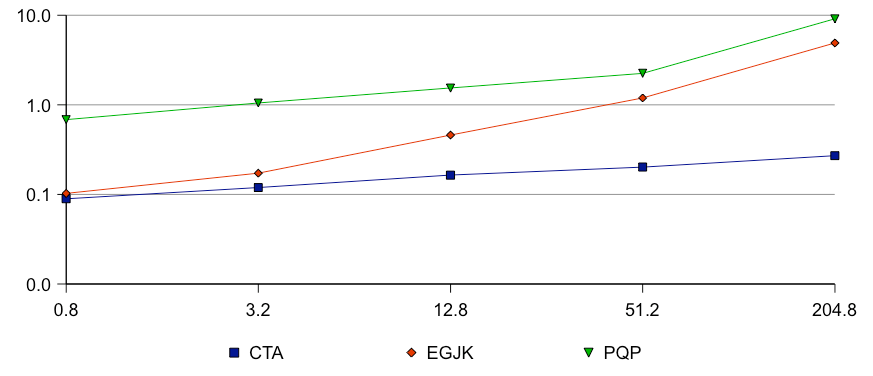
\includegraphics[width=\hsize]{Carpin_Figure_CTA.pdf}
    \mycaption{Time spend to solve a collision query as a function of
    the complexity of the involved polyhedra. The blue line outlines
    the performance of the proposed algorithm.}
    \label{fig:Carpin_pic1}
\end{center}
\end{figure}





\paragraph{Organization}

\begin{enumerate}
    \item 6th IEEE International Workshop on Robot Motion and  Control: program committee
          member
   \item IEEE 2006 International Conference  on Information Reuse  and
Integration: program committee member
\item PerMIS 2006: program committee member
   \item 6th international joint conference on autonomous agents and multiagent
          systems: program committee member
\item Robocup Federation: elected Executive Member for the 2007-2009 term
\item Organizer of  a tutorial on "USARSim/MOAST: Highly Realistic Simulation and Control for Multi Robot" held at the IEEE International
Conference on Robotics and Automation (Orlando-FL, May 2006)
\item Organizer of a tutorial on "USARSim and MOAST: Advanced Tools for High-Fidelity Simulation of Distributed Robot Systems "   held at the annual conference
of the American Association for Artificial Intelligence  (Boston-MA, July 2006)
\end{enumerate}

\paragraph{Collaborations}
\begin{enumerate}
    \item {\sl National Institute of Standards and Technology, USA}\\
          Dr. Steve Balakirski\\
          Organization of the Virtual League Competion and development of USARSim
    \item {\sl University of Pittsburgh, USA}\\
          Prof. Mike Lewis\\
          Organization of the Virtual League Competion
    \item {\sl University of Udine, Italy}\\
          Prof. Claudio Mirolo\\
          Development of Algorithms for Collision Detection
    \item {\sl University  of Padova, Italy}\\
          Prof. Enrico Pagello\\
          Development of Algorithms for Multi-Robot Motion Planning
\end{enumerate}



%\paragraph{Publications}

%\begin{description}
 % \item[Journals]
 \nocite{Carpin:IEEEPRO2006}\nocite{Carpin:ACTA2006}\nocite{Carpin:AR2006}

 % \item[Conference Proceedings]
  \nocite{Carpin:IAS2006}\nocite{Carpin:RS1}\nocite{Carpin:RS3}
  \nocite{Carpin:PerMIS2006b}\nocite{Carpin:PerMIS2006a}\nocite{Carpin:ICRA2006GM}
  \nocite{Carpin:ICRA2006BCMOMMT}
 % \item[Books/Collections]
   \nocite{Carpin:LNCS4123}
%\end{description}
%\end{document}
%%% Local Variables:
%%% mode: latex
%%% TeX-master: "report"
%%% End:

  \putbib[combined]
\end{bibunit}
\shorttitle{Microelectronic Devices and Technologies}
\subsection{Microelectronic Devices and Technologies}

To continue the rate of progress in information and systems and
technologies into the next decade fundamental questions in material
science and manufacturing technology have to be answered to further
reduce the device dimension into the sub 100nm arena and increase
the complexity of integrated circuits. Novel Micro and Nano
Technologies are needed, either to overcome limitations to further
shrinking of devices and/or to implement novel electronic
hardware/services (such as large flexible displays). In parallel to
the development of novel devices, the integration into large volume
manufacturing processes and the specific problems associated to
manufacturing and quality/reliability engineering of these have to
be addressed, according to the principles of concurrent engineering.

%%% Local Variables:
%%% mode: latex
%%% TeX-master: "report"
%%% End:

\begin{bibunit}[hplain]
  \subsubsection{Electronic Devices and Nanophotonics}
\index{Knipp, Dietmar}

\paragraph{Electronic Devices and Nanophotonics group}
Dietmar Knipp (Professor), Amare Benor, Kah-Yoong Chan, Christian Haase (external PhD
student)  (PhD Student), Rahul Dewan (MSc student), Zhelio Andreev (MSc student)\\

Research of the Electronic Devices and Nanophotonics group is
focused on nano and optical technologies and their applications in
information technology and photovoltaics. The major goal of the
research is to develop the next generation of electronic and
photonic devices bridging from the micro to the nanoscale.

\paragraph{Highlights}

With the advent of micro and nano fabrication the production of nano-structured materials
in the sub 100 nm range became feasible. Such nanostructures are of interest for several
optical and photonic applications like solar cells and optical sensors.  For example, the
conversion efficiencies of thin film solar cells can be increased by nano texturing of the
cells. Due to nano texturing a larger fraction of the incoming light is scattered and
diffracted, so that the total absorption of light in the solar cell is
enhanced. Subsequently the generated photocurrent and the conversion efficiency of the
solar cell are enhanced. Despite these improvements the underlying optics in such nano
textured solar cells is not fully understood. Classical optics does not facilitate the
description of the wave propagation in such a solar cell. Maxwell's equations have to be
solved in 2D or 3D to gain insights in the optical wave propagation of such devices.  The
optics were studied by numerical simulations using a Finite Integration Technique (FIT)
and Finite Difference Time Domain (FDTD) approach. The device structure is approximated by
a solar cell with a periodic groove structure. The Figure~\ref{fig:profknipp1} (left)
shows one period of such a solar cell with a groove structure. The numerically simulated
absorption is shown in Figure~\ref{fig:profknipp1}, right.

\begin{figure}[ht]
  \begin{center}
    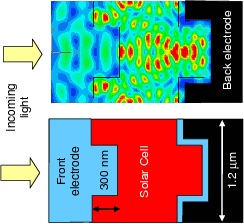
\includegraphics[width=\hsize, angle=270]{profknipp-figinfo.png}
    \mycaption{ Cross section of a slice of a nanotextured solar cell (left) and
      absorption profile in the solar cell}\label{fig:profknipp1}
   \end{center}
\end{figure}


The absorption of light in the cells is increased, due to scattering and diffraction of
light. Simulations carried out by Christian Haase show that the grooves cause an increase
of the total conversion efficiency of
10-15\%.
%The increase of the absorption is mainly observed for the infrared part of the
%optical spectrum. Based on a comparison of the experiment and the numerical
%simulation an optimized nano patterning schemes can be derived. The simulations show
%that the conversion efficiency is maximized if the height of the grooves is
%approximately equal to half of the period of the grooves.
The optical simulations were not only applied to solar cells. Numerical simulation of
metallic nanostructures shows that metallic hole arrays can be applied as optical
filters. The filter properties can be tuned by changing the diameter and the spacing of
the holes in the metal film. As the fabrication of the metallic structures is compatible
with classical micro and nanoelectronics such metallic nanostructures can be integrated in
conventional optical sensor or digital cameras. Cameras using such metallic nanostructures
would exhibit a reduced pixel cross talk and a higher spectral resolution.  In summary,
optics on the nanoscale provides a lot of new opportunities for technical
applications. Numerical simulations of the optics on the nanoscale are essential to gain a
solid understanding and optimize the device structures. In order to verify the results of
numerical simulations have to be compared to experimental results.  The research on
optics in nanostructured media is carried out in close collaboration with the research
group of Dr. H. Stiebig at the Institute of Photovoltaics, Research Center J\"ulich.

\paragraph{Collaborations}
\begin{enumerate}
\item {\sl International University Bremen} \\ Prof. Veit Wagner \\ Organic Electronics
\\ Prof. Werner Bergholz \\ Photovoltaics and Microelectronics
\item {\sl University Bremen} \\ Prof. Wolfgang Benecke \\ Microsystems Technology
\item {\sl Research Center J�lich} \\ Dr. Helmut Stiebig \\ Nanocrystalline Thin Film
  Transistors and Optics in nanostructured media
\item {\sl Bendit Innovative Interfaces} \\ J. Huyer \\ Solar Cells for mobile
  applications
\item {\sl Palo Alto Research Center} \\ Dr. R.A. Street, A.R. V�lkel. Dr. J. Northrup \\
  Organic electronics and modelling
\item {\sl Stanford University} \\ Prof. A. Salleo \\ Organic electronics

\end{enumerate}


\paragraph{Grants}
% list the running grants in 2006, if none have been received, please delete this
% subsection.
\begin{enumerate}
%\item {BMBF} ``Embedded Microsystems Bremen (EMB)''
\item Funded by {Forschungszentrum J\"ulich}, \emph{Funktionale
Kontaktschichen}, (February 2006 - January 2007)
\end{enumerate}


\paragraph{Awards, Prizes}
% list the grants you have received in 2005, if none have been received, please delete
% this subsection.
\begin{enumerate}
\item Ernst A.C. Lange Award together with Prof. W. Benecke from the Institute for
  Microsensors, -actuators, and -systems (University Bremen)
\end{enumerate}

\paragraph{Patents}
\begin{enumerate}
\item H. Stiebig, D. Knipp, J. F�lsch, Three-color sensor with a pin or nip series of
  layers, Japan, Patent number: Hei-9-535750;
\item D. Knipp, Optical sensor and integrated photonic crystal and method for producing
  the optical sensor, submitted to German patent office.
\end{enumerate}


\nocite{Knipp1, Knipp2, Knipp3, Knipp4, Knipp5, Knipp6, Knipp7, Knipp9,
Knipp10, Knipp11, Knipp13}

  \putbib[combined]
\end{bibunit}
\begin{bibunit}[hplain]
  
\subsubsection{Microelectronics}\label{ict:micro:bergholz}
\index{Bergholz, Werner}

\paragraph{Research Team}
Werner Bergholz (Professor), Thomas Dinkel (PhD student), Uwe Pagel (Technical
Assistant)\\

%%% give a very short (150 words description of your research area)
%% Hint: this can be copied from the research areas document (../masterplan/research-areas)

After 30 years of rapid advancements in microelectronics barriers are emerging for a
further device shrink and/or improvement of quality/failure rates. Our research focuses on
these ``brick walls''. These barriers are mainly related to defects, which limit yield and
reliability and the exploding cost for lithography. In addition, nanotechnology artefacts,
such as carbon nano tubes and quantum dots are getting closer to integration into
conventional microelectronic products. The specific research topics are the
\begin{myitemize}
\item Development of destruction free methods to detect defects in silicon wafers
\item Defect-related failure mechanisms and reliability test methods for microelectronic
  circuits.
\item New wafer types with functional layers to mitigate the cost explosion for
  lithography
\item Novel process control methodology to improve quality and productivity.  Unless
  solutions for the listed challenges can be identified, the rapid expansion of
  information technology will slow down within the next 5 years.  In addition, the
  following additional research topics are being addressed,
\item Investigation of defect engineering methods and efficiency detractors in Si solar
  cell technology (based on an synergy with microelectronics techniques)
\item Application of Quality Management methodology and standardisation techniques to
  nanotechnology and other non-technical areas.
\end{myitemize}
One of the more subtle limitations to further device shrink is a phenomenon known as
random telegraph signals (RTS noise) in semiconductor devices. Known and not understood
for more than 30 years, it never had particular technological importance. With devices in
the 100nm size range or below, it is gradually transforming from a laboratory curiosity to
a serious challenge in many application areas.

\begin{figure}[ht]
  \begin{center}
      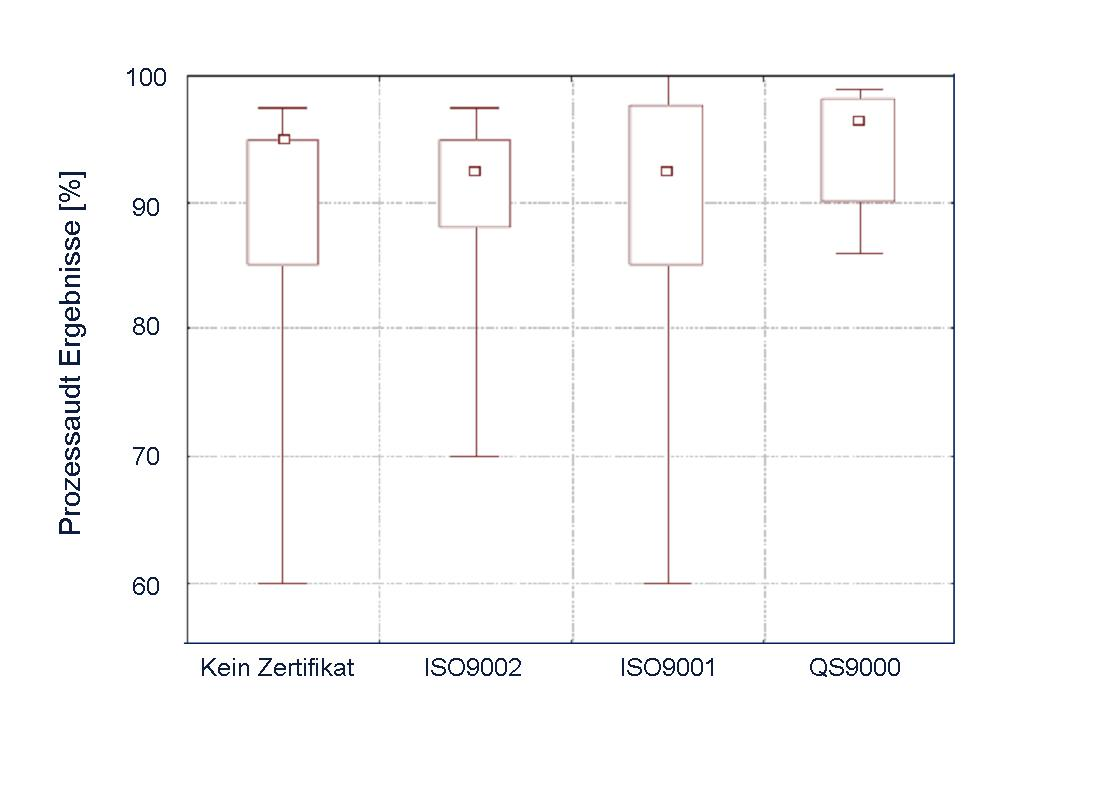
\includegraphics[width=\hsize]{EECS/bergholz-fig1}
    \mycaption{Boxplot comparison of the scores in a process-oriented audit of suppliers
      to the microelectronics industry. Suppliers which conform to the QS9000 (TS16949)
      Quality standard are clearly superior to ISO9000 certified or not certified
      companies}
    \label{fig:switching}
   \end{center}
\end{figure}

\paragraph{Highlights}

{\emph{Quality Management methodology}}: An evaluation of about 100 second party audits of
materials suppliers to the microelectronics industry has shown that a certification
according to the quality management standard TS16949 (formerly QS9000) correlates with
positive results in a process oriented audit methodology (see Fig.~\ref{fig:switching}). On
the other hand, certification according to the standard ISO9001 and ISO9002 (less
stringent than TS16949) does not guarantee a sufficient quality level, if it is compared
to the former group or companies which have no certification at all. There are also
significant differences between silicon wafer manufacturers (which have a decade long
tradition in clean room technology and high quality standards) and producers of other
materials for the Chip industry (chemicals, gases, metals etc.). Furthermore, it can be
concluded that the process oriented audit methodology is a sutiable tool to measure the
quality standard of a
supplier.\\

{\emph{Random Telegraph Signals in Si devices}}: The study of random telegraph signals in
diodes has been extended to the influence of temperture bias stress measurements
(S. Nandhavel \& W. Bergholz). After 175 degrees C (Fig.~\ref{fig:leakage}) leakage can be
observed, which is consistent with the hypothesis that metal boron pairs are the
responsible defects. Deep Level Transient Spectroscopy, radiation experiments and TEM
studies are planned to track down the defect mechanism.

{\emph{Photovoltaics industry}}: A systematic study of the open data for the process
capabilities of all major PV manufacturers has revealed an unexpected large variation in
the efficiencies and other performance indicators. It is planned to identify methods how
the process variation can be reduced by "copy intelligently" of engineering methods
developed in the microelectronics industry.

\begin{figure}[ht]
  \begin{center}
    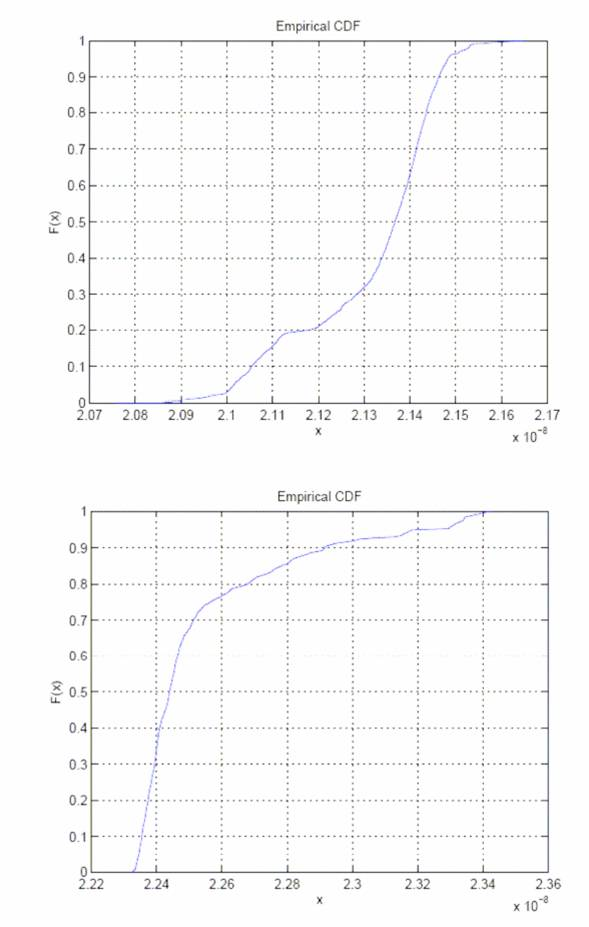
\includegraphics[width=7cm]{EECS/bergholz-fig2}
    \mycaption{After temperature bias stress of a diode there is a reversible recovery of
      the leakage currents for voltages slightly below the barrier voltage, attributed to
      diffusion pairing reactions of metal impurities, comparison of the cumulitive
      distribution function for the leakage curents before and after stress at 175 degrees
      C}
    \label{fig:leakage}
   \end{center}
\end{figure}

{\bf Outlook}: It is planned to supplement the study on audit methodology to a correlation
with a performance evaluation of the same suppliers and to extend the study to the data
gathered by a major car manufacturer in about 10 000 quality audits at suppliers to the
car industry. Objective: further refine the audit methodology and quality management
implementation methods. The Study on RTS will be extended to the investigation of methods
to reduce the effect and thus lower or remove one of the roadblocks to the
microelectronics industry. The long term goal of the PV studies is to develop efficient
defect reduction and efficiency optimization methods so as to support the goal for cost
reduction by a factor or 3 until PV becomes competive for peak power in grid
applications. The standardisation research in cooperation with DIN, DKE and SEMI is
targetted towards early anticipatory standards in emerging nanotechnology to facilitate
the transformation from lab to fab.

%\newpage
\paragraph{Organization}
\begin{enumerate}
\item Workshop: ``Silicon Wafers SEMI� Standards Workshop'', April 05 2006, Munich Trade
  Center
\item SEMI Autumn Conference: ``Conference "Bridging Semiconductor \& Related'', 08th
  Nov2006 Dresden
\end{enumerate}
\paragraph{Collaborations}
\begin{enumerate}
\item {\sl Infineon Technologies, Dresden}\\
  RTS noise phenomena
\item {\sl Infineon Technologies, Munich}\\
  Test Set up for DRAMs
\item {\sl MEMC, St. Peters, Missouri}\\
  Defect Detection in Silicon Wafers
\item {\sl Q-Cells, Thalheim}\\
  Efficiency Engineering for Silicon-based Solar Cells
\item {\sl Quintiq, S'Hertogenboch, Netherlands}\\
  Best practice Quality Management Tools for the Software Industry
\item {\sl International University Bremen}\\
  Dietmar Knipp\\
  Solar cells, low cost electronics
\item {\sl International University Bremen}\\
  Peter Ludes (SHSS), C. Schwender (JCLL)\\
  Visual mass communication
\item {\sl SEMI (Semiconductor Equipment and Materials)
    San Jose, Brussels}\\
  Bettina Weiss, Carlos Lee\\
  Semiconductor Standards Development
\item {\sl DIN, Berlin}\\
  Standardization of Nanomaterials
\item {\sl DKE, Frankfurt, Main}\\
  Standarization of Nanoelectronic Electronic Products
\end{enumerate}

\paragraph{Patents}
\begin{enumerate}
\item Patent on wafer technology, in the filing process
\end{enumerate}

\paragraph{Grants}
 \begin{enumerate}
\item Funded by Deutsches Institut f�r Normung (DIN/DKE) /
Bundesministerium f�r Wirtschaft,  \emph{Standardisierung
Nanoelektronik} (July - December 2006)
\end{enumerate}

\paragraph{Awards, Prizes}
\begin{enumerate}
\item shortlisted for the IEC centinary Award Challenge
\end{enumerate}

\newpage
%\paragraph{Publications}
%\nocite{BerWeiLee:QFD05}
%\nocite{KumWeiPagBer:ecrtnd05}
%\nocite{BaaBerg:ddf05}
\nocite{WittBerg:wbqz06}
\nocite{Berg:msinpb06}
\nocite{BergWeLee06}


%\end{description}
%\end{document}
%%% Local Variables:
%%% mode: latex
%%% TeX-master: "report"
%%% End:

  \putbib[combined]
\end{bibunit}

% %Life Sciences
% %%%%%%%%%%%%%%%%%%%%%%%%%%%%%%%%%%%%%%%%%%%%%%%%%%%%%%%%%%%%%%%%%%%%%%
\cleardoublepage


%\shorttitle{Life Sciences}
%\section{Life Sciences}
\shorttitle{Life Sciences}
\section{Life Sciences}

\begin{figure*}[ht]
  \begin{center}
   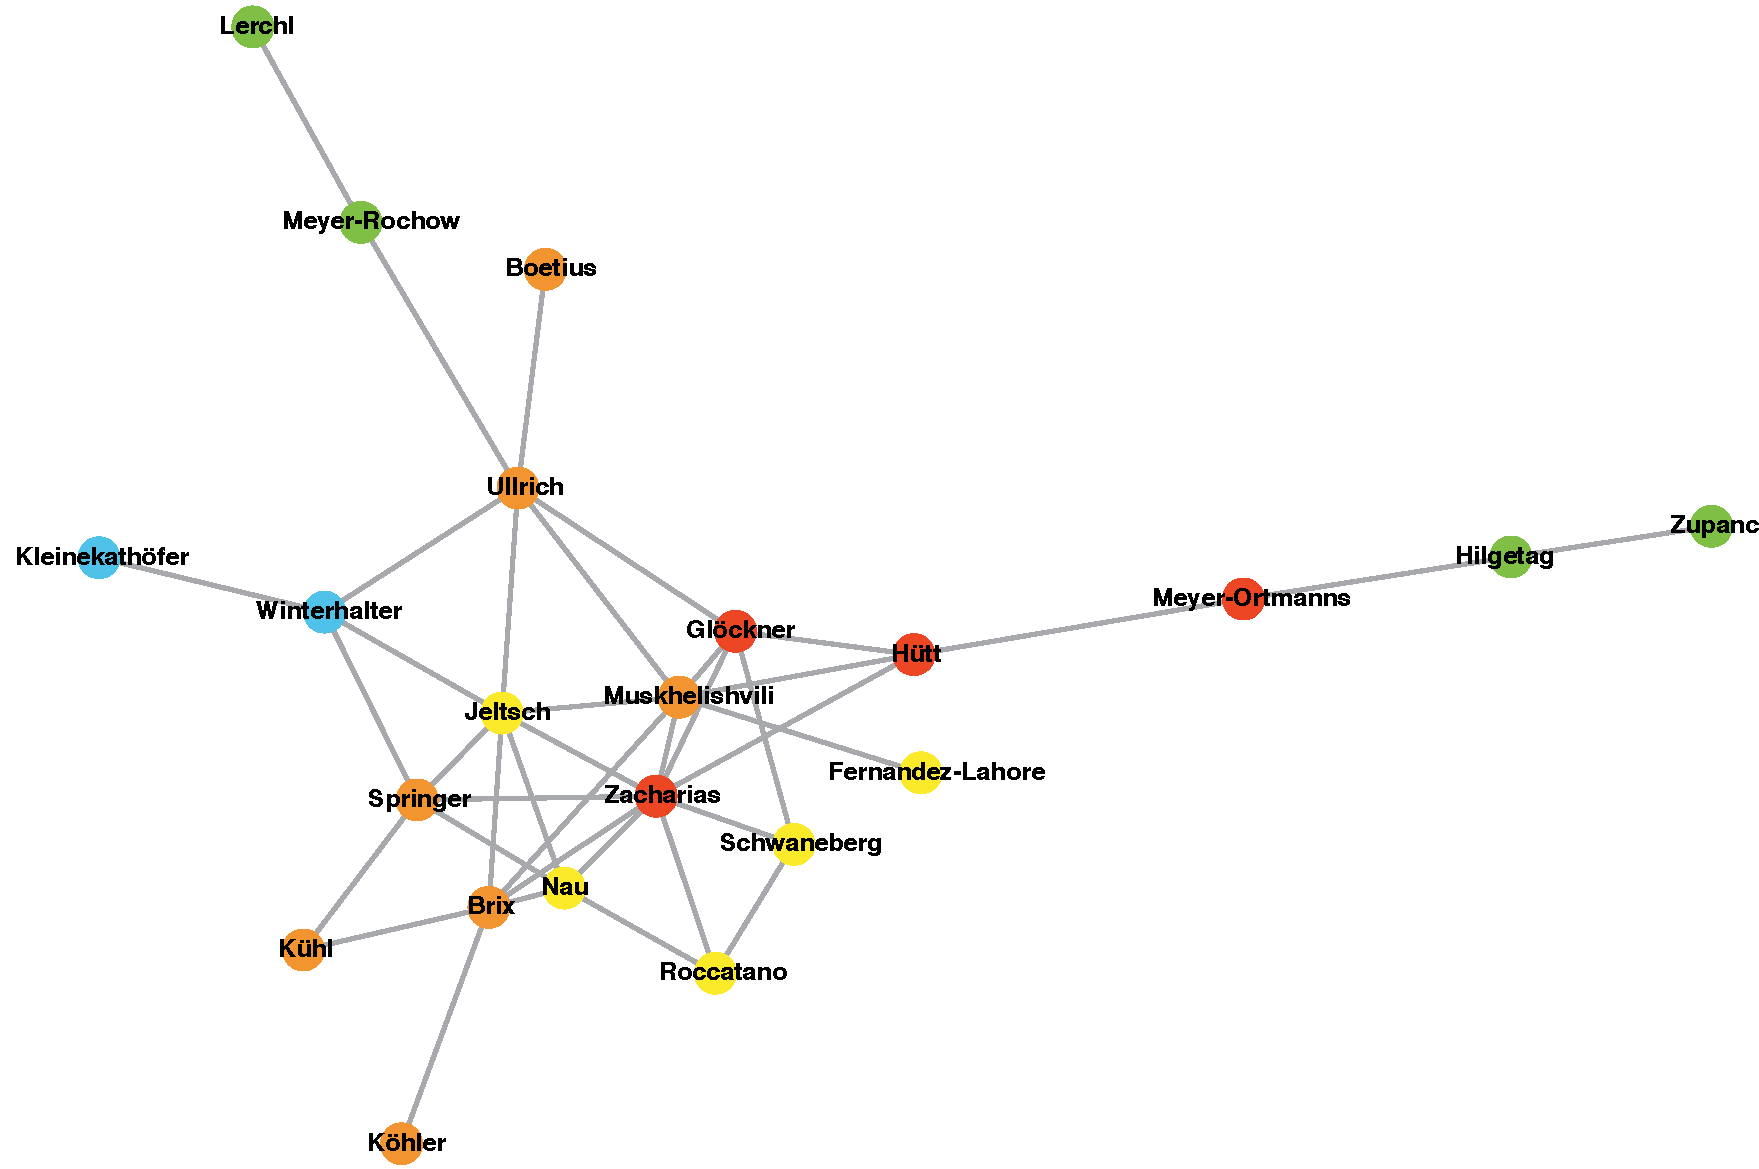
\includegraphics[width=\hsize]{network_LifeSci1_tmp03.pdf}
    \mycaption{Geometry and functionality of the complex biological network at Jacobs University Bremen that is formed by the interaction of Computational Biologists, Biophysicists, Biotechnologists, Neuroscientists, and Molecular Life Scientists.  }\label{fig:LifeSc}
   \end{center}
\end{figure*}


Life Scientists at IUB follow an integrated research approach that covers a variety of scientific fields and interests. The spectrum ranges from the analysis of molecules and their usage for biotechnological applications to the understanding of the mechanisms that explain the functions of complex systems like cells, organisms, and even entire habitat communities. Our research approaches combine experimental and theoretical work aiming towards future challenges in the target areas of the School of Engineering and Science. \\

The Life Scientists at IUB focus their research interests on
\begin{myitemize}
\item   the molecules and macromolecules which make up living matter,
\item the dynamical organization of genomes and cells,
\item   the biochemistry and physiology of life,
\item   the molecular mechanisms that maintain vital functions of cells, and
\item   the patho-physiological events which result in the onset of diseases.\\
\end{myitemize}


The research results provide us with insights into the molecular mechanisms that are found in microbes, plants and animals. Moreover, marine and terrestric habitats which are filled with life are analyzed in composition and interactivity. The perception of animals and human beings of their surrounding world is another important aspect of our research teams as is the modeling of complex systems like gene networks, metabolism, trafficking of molecules in cells, and interaction of living creatures in biological systems.\\

In 2006, a clear focus was on the spatial and temporal regulation of biological systems. Another important and recent advance is that the Molecular Life Scientists at IUB have filled their excellently designed and newly build research facilities and laboratories with life. Life Scientists at IUB have established numerous successful research collaborations within our research community. Above it, our research activities are embedded in the scientific communities of the Bremen-area and have attracted significant international attention. The nodes and edges that make up the units of the vital network of Life Scientists at IUB are illustrated in Figure \ref{fig:LifeSc}. \\




\textit{Perspectives}\\
The goal of the Life Scientists at IUB is to understand the function
of life, in its complexity and functional organization, on the
molecular and the systemic levels. We feel best prepared to further
evolve our research activities to face the major global challenges
of the future.




\shorttitle{Computational Biology}
\subsection{Computational Biology}

Computational Biology at IUB uses numerical simulations, novel data analysis concepts and mathematical modeling to better understand biological data. These computational approaches allow relating information from very different levels of organization: e.g., protein binding and protein networks, genomes and ecology, regulation and patterns.\\

In 2006 the fields of research have been extended towards Systems Biology and now cover all major research areas of Computational Biology. The output of Computational Biology during this year ranges from articles in high-ranking scientific journals, scientific textbooks, software tools to the organization of conferences and summer schools. Progress has been made in analyzing metagenomic data, including flexibility in binding processes of biomolecules and understanding dynamic processes on abstract and real biological networks.\\

Bridging scales is the essence of a system-wide understanding and, at the same time, a source of a wide range of scientific collaborations. The vast methodological knowledge involved is relevant to virtually all parts of the life sciences. Work on Computational Biology is well embedded in the Complex Systems focus of Jacobs University.\\


\begin{bibunit}[hplain]
\subsubsection{Ecological Genomics}
\index{Gl�ckner, Frank Oliver}

\paragraph{Research Team}
%
Frank Oliver Gl�ckner (Professor), Marga Bauer (Postdoc), Thierry Lombardot (Postdoc), Francesca Simonata (Postdoc), Hanno Teeling (Postdoc),  Marcel Huntemann (PhD Student), Renzo Kottmann (PhD Student), Christian Quast (PhD Student), Michael Richter (PhD Student), Patricia Wecker (PhD Student), J�rg Peplies (Guest), Andreas Ellrott (Technical Assistant), Carsten Witt (Technical Assistant)\\

The advent of high throughput sequencing technologies in the last years enables to unravel the diversity and function of marine microorganisms on a whole genome level. It's the objective of Genome Bioinformatics to take advantage of this development and learn more about the mechanisms coded in the genome enabling the organisms to adapt to changing environmental conditions. To reveal the relevant genes and their functions an integrative approach is followed to correlate sequence data with information about gene expression, habitat-specific parameters and microbial diversity. This in turn should uncover specific niche adaptations and give hints how the organisms influence the global cycling of matters. The knowledge obtained will lead to a better understanding of the complexity, interactions and stability of marine habitats. The long-term perspective is to predict the impact of the ongoing global changes on the marine ecosystem.

\paragraph{Highlights}


\textit{Genomics and Metagenomics}
One of the highlights in 2006 was the contribution to the paper by Woyke et al. which came out in Nature recently. In this metagenomic paper random shot gun sequencing was used to address the metabolic potential of the symbiotic community of the marine worm \textit{Olavius algarvensis}. Besides enhanced functional annotation, we were able to further address the binning problem, which is central to any metagenomic project. Binning means the bioinformatic assignment of the sequence fragments back to the organisms in the sample. The problems are: 1. the sequence fragments that carry the metabolic genes of interest often lack suitable markers for their phylogenetic classification, and 2. fragments from the same organism can not be reliably identified as such, unless they overlap. The tool TETRA (www.megx.net/tetra) has been developed to address this task based on intrinsic sequence signatures and successfully applied in several projects. Since it is limited to fragment sizes above 20-30 kb we have further developed the system to enhance sensitivity. The new MetaClust system is now able to deal with fragment sizes down to 5 kb. A prototype of the new system was evaluated within the \textit{O. algarvensis} project and the four expected symbiotic genomes could be clearly differentiated (see Figure \ref{fig:gloeckner-fig1}).
Additionally, we could finish four genome projects that provided new insights into the life-style of three marine bacteria and one marine phage. All projects have been performed in close collaboration with national and international partners from the Network of Excellence Marine Genomics Europe and the Joint Genome Institute in the US.

Within the framework of our EU-project MetaFunctions (www.metafunctions.org) we were able to significantly enhance the integrative database and our visualization tools provided by the `Genomes Mapserver' (www.megx.net/mm). The idea behind MetaFunctions is to integrate sequence data with habitat parameters using the geographic information system (GIS). The ultimate aim is to use novel data-mining systems that help determining functions of those genes for which the activity is not yet known. Hundred thousand of scientific publications and the public sequence repositories are now screened by our partners for relevant information. A variety of natural language processing algorithms are being tested to collate this data and convert it into our structured, database format. Analytical tools like MetaLook are under development to enable the project team and later scientists around the world to clearly visualize the results of diverse analyses.
\begin{figure}[ht]
  \begin{center}
   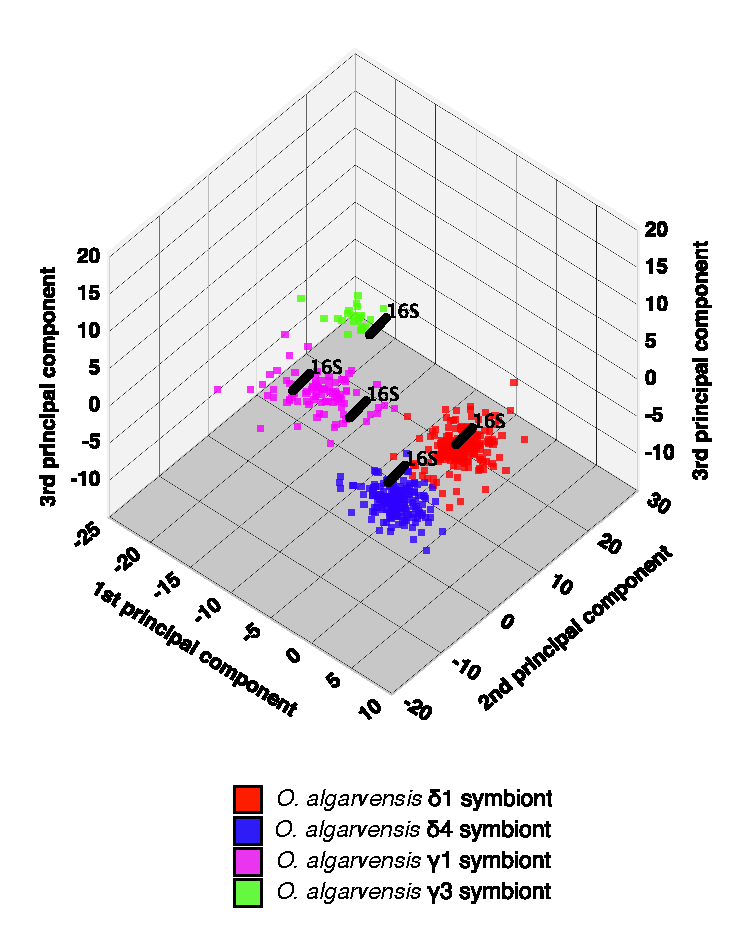
\includegraphics[width=\hsize]{Gloeckner/Gloeckner-fig1.pdf}
    \mycaption{Clustering of the \textit{O. algarvensis} symbiont scaffolds. Visualization
of the first three components of a principal component analysis, in
which GC-content, net-read-depth z-scores for all possible 64
trinucleotides and 256 tetranucleotides were incorporated with equal
weight (z-scores calculated with TETRA, and normalized by length).
The colours represent the four clusters of scaffolds (calculated
with MetaClust). }\label{fig:gloeckner-fig1}
   \end{center}
\end{figure}

\textit{Microarray analysis}
Systematic studies have been conducted to address the issue of nonspecific target binding. This was possible in collaboration with Dirk Sch�ler from the MPI-Bremen since he was able to provide the isogenic deletion mutant MSR-1B of \textit{Magnetospirillum gryphiswaldense}. This model system was used to systematically investigate the amount of false positive hybridization events. Finally, a three colour hybridization assay was developed to compare MSR-1B culture and two MSR-1 wild type cultures grown under different conditions. The results show that common microarray platforms still suffer from a significant amount of unspecific signals even under optimal hybridization conditions.



\paragraph{Organization}
%
\begin{enumerate}
\item EU-workshop Bioinformatics I - Introduction to Sequence and Genome Analysis in collaboration with the Ribocon GmbH (January 23-27)
\item Extended international phylogeny (ARB) workshop in collaboration with the Ribocon GmbH (May 30 - June 02)
\item International Exploratory Workshop: ``Marine Genomics meets Marine Diversity'' (June 07-09)
\item International phylogeny (ARB) workshop in Z�rich in collaboration with the Ribocon GmbH (September 19-22)
\item International phylogeny (ARB) workshop in collaboration with the Ribocon GmbH (November 28 - December 02)
\end{enumerate}

\myparagraph{Collaborations}
%
Bremen Area Collaborations:
\begin{enumerate}
\item {\sl International University Bremen} \\ Prof. M.-Th. H�tt \\ Genome signatures
 \\ Prof. G. Muskhelishvili \\ Transcriptomics
\\ Prof. M. Ullrich \\Expression profiling
\\ Prof. M. Zacharias, Prof. U. Schwaneberg\\ Sulfatases
\item {\sl Universit�t Bremen} \\ Prof. O. Herzog \\ Bioinformatics
\item {\sl TTZ Bremerhaven} \\ Dr. U. Bohnebeck \\ MarMic, Metafunctions
\item {\sl University Hamburg} \\ Prof. S. Kurtz \\ Genomics
\item {\sl Alfred-Wegener-Institut Bremerhaven} \\ Wilshire \\ LTER
\end{enumerate}
National \& International Collaborations:
\begin{enumerate}
\item {\sl Technische Universit�t M�nchen} \\ Dr. W. Ludwig\\ Bioinformatics, ARB, ARB-Genome
\item {\sl Universit�t Bielefeld} \\ Prof. A. P�hler, Dr. A. Becker\\ Bioinformatics, GenDB, microarrays
\item {\sl University W�rzburg} \\ Dr. U. Hentschel\\ Phylogeny
\item {\sl Max-Planck-Institut f�r molekulare Genetik, Berlin} \\ Dr. R. Reinhard\\ Genome sequencing
\item {\sl Rechenzentrum der MPG Garching} \\ Dr. H. Lederer\\ Bioinformatic pipeline
\item {\sl Bundesanstalt f�r Gew�sserkunde} \\ Dr. W. Manz\\ Microarrays
\item {\sl University of the Balearic Islands} \\ Prof. R. Rossello-Mora\\ Molecular taxonomy and ecology, Salinibacter
\item {\sl University of Alicante} \\ Prof. P. Anton\\ Salinibacter
\item {\sl Station Biologique Roscoff} \\ Dr. G. Michel\\ Zobellia
\item {\sl CBS Danmark} \\ Prof. D. Ussery\\ genome comparison
\item {\sl Woods Hole Marine Biological Laboratory} \\ Prof. M. Sogin, D. L-A. Zettler\\ ICoMM
\item {\sl UNEP/GRID-Europe} \\ Dr. J. Jaquet \\ Metafunctions
\item {\sl Poznan University of Technology} \\ Prof. J. Blazewicz \\ Metafunctions
\end{enumerate}

\paragraph{Grants at the Max Planck Institute for Marine Microbiology}
\begin{enumerate}
\item EU-NoE Marine Genomics Europe (GUCE-CT-2004-505403)
\item EU-project MetaFunctions (511784-2)
\end{enumerate}

\goodbreak

\nocite{Gloeckner1,Gloeckner2,Gloeckner3,Gloeckner4,Gloeckner5,Gloeckner6,Gloeckner7,Gloeckner8,Gloeckner9,Gloeckner10,Gloeckner11,Gloeckner12}

\putbib[combined]
\end{bibunit}

\begin{bibunit}[hplain]
\subsubsection{Biomeolecular Modeling}
\index{Zacharias, Martin}

\paragraph{Research Team}
%
Martin Zacharias (Professor), Andr\'{e} Barthel (Postdoc), Andreas May (PhD Student), Florian Sieker (PhD Student), J\'{e}r\'{e}my Curuksu (PhD Student), Srinivasaraghavan Kannan (PhD Student)\\


The research focus of the Computational Biology group is the study of biomolecular
association and conformational flexibility using computer simulation approaches.
The simulation studies are aimed to better understand structure formation of
biomolecules and the mechanism of ligand-receptor association. As the major
computational tool we employ the molecular dynamics simulation method to investigate
the structure and dynamics of proteins and nucleic acids at atomic resolution.
We also develop new docking approaches that allow to predict putative binding sites
for ligands and inhibitors on the surface of biological target molecules.
The prediction of putative ligand binding geometries and binding sites on a
biomolecule is of tremendous importance for the design of new drugs that can bind
and interfere with the function of biomolecules. Focus of another research area is
to improve comparative protein structure modeling. Improving the accuracy of
structural modeling of proteins is also of central importance to use such structural
models for drug design. In close collaboration with experimental groups the
computational approaches are applied to several biologically important targets.

\paragraph{Highlights}

\null{\sl Conformational Dynamics of Nucleic Acids }

The conformational flexibility of DNA is central to its many biological functions including recognition by proteins during gene regulation, DNA repair, packaging in the cell and transient melting during transcription and replication. Specific binding by proteins is not only determined by specific interactions between DNA and proteins but also by the sequence-dependent structure and deformability of the DNA helix. The DNA twist flexibility is of particular importance since it plays a role during supercoiling and packing of DNA. We have designed a method to induce twist deformations in DNA during simulations and to record associated free energy changes. Simulations allowed to extract free energy profiles for twist deformations and were performed on a series of DNA dodecamer duplexes. The shape of the free energy curves was similar for all duplexes. The calculated twist deformability was in good agreement with experiment and showed only modest variation for the complete duplexes. However, the response of the various base pair steps on twist stress was highly non-uniform. In particular, pyrimidine/purine steps were much more flexible than purine/purine steps followed by purine/pyrimidine steps. This non-uniform local response may significantly alter the shape of the DNA recognition surface which in turn can affect binding of proteins and other ligands as a result of external twist stress. It was also possible to extract correlations of twist changes and other helical as well as global parameters of the DNA molecules. Severe un-twisting of DNA below an average of 25 degrees per base-pair step resulted in the onset of a global structural transition with a significantly smaller twist at one end of the DNA compared to the other end. (Fig.~\ref{fig:twist}) The effect of DNA damage and binding of ligands on the twist deformability will be subject of future studies.


\begin{figure}[ht]
  \begin{center}
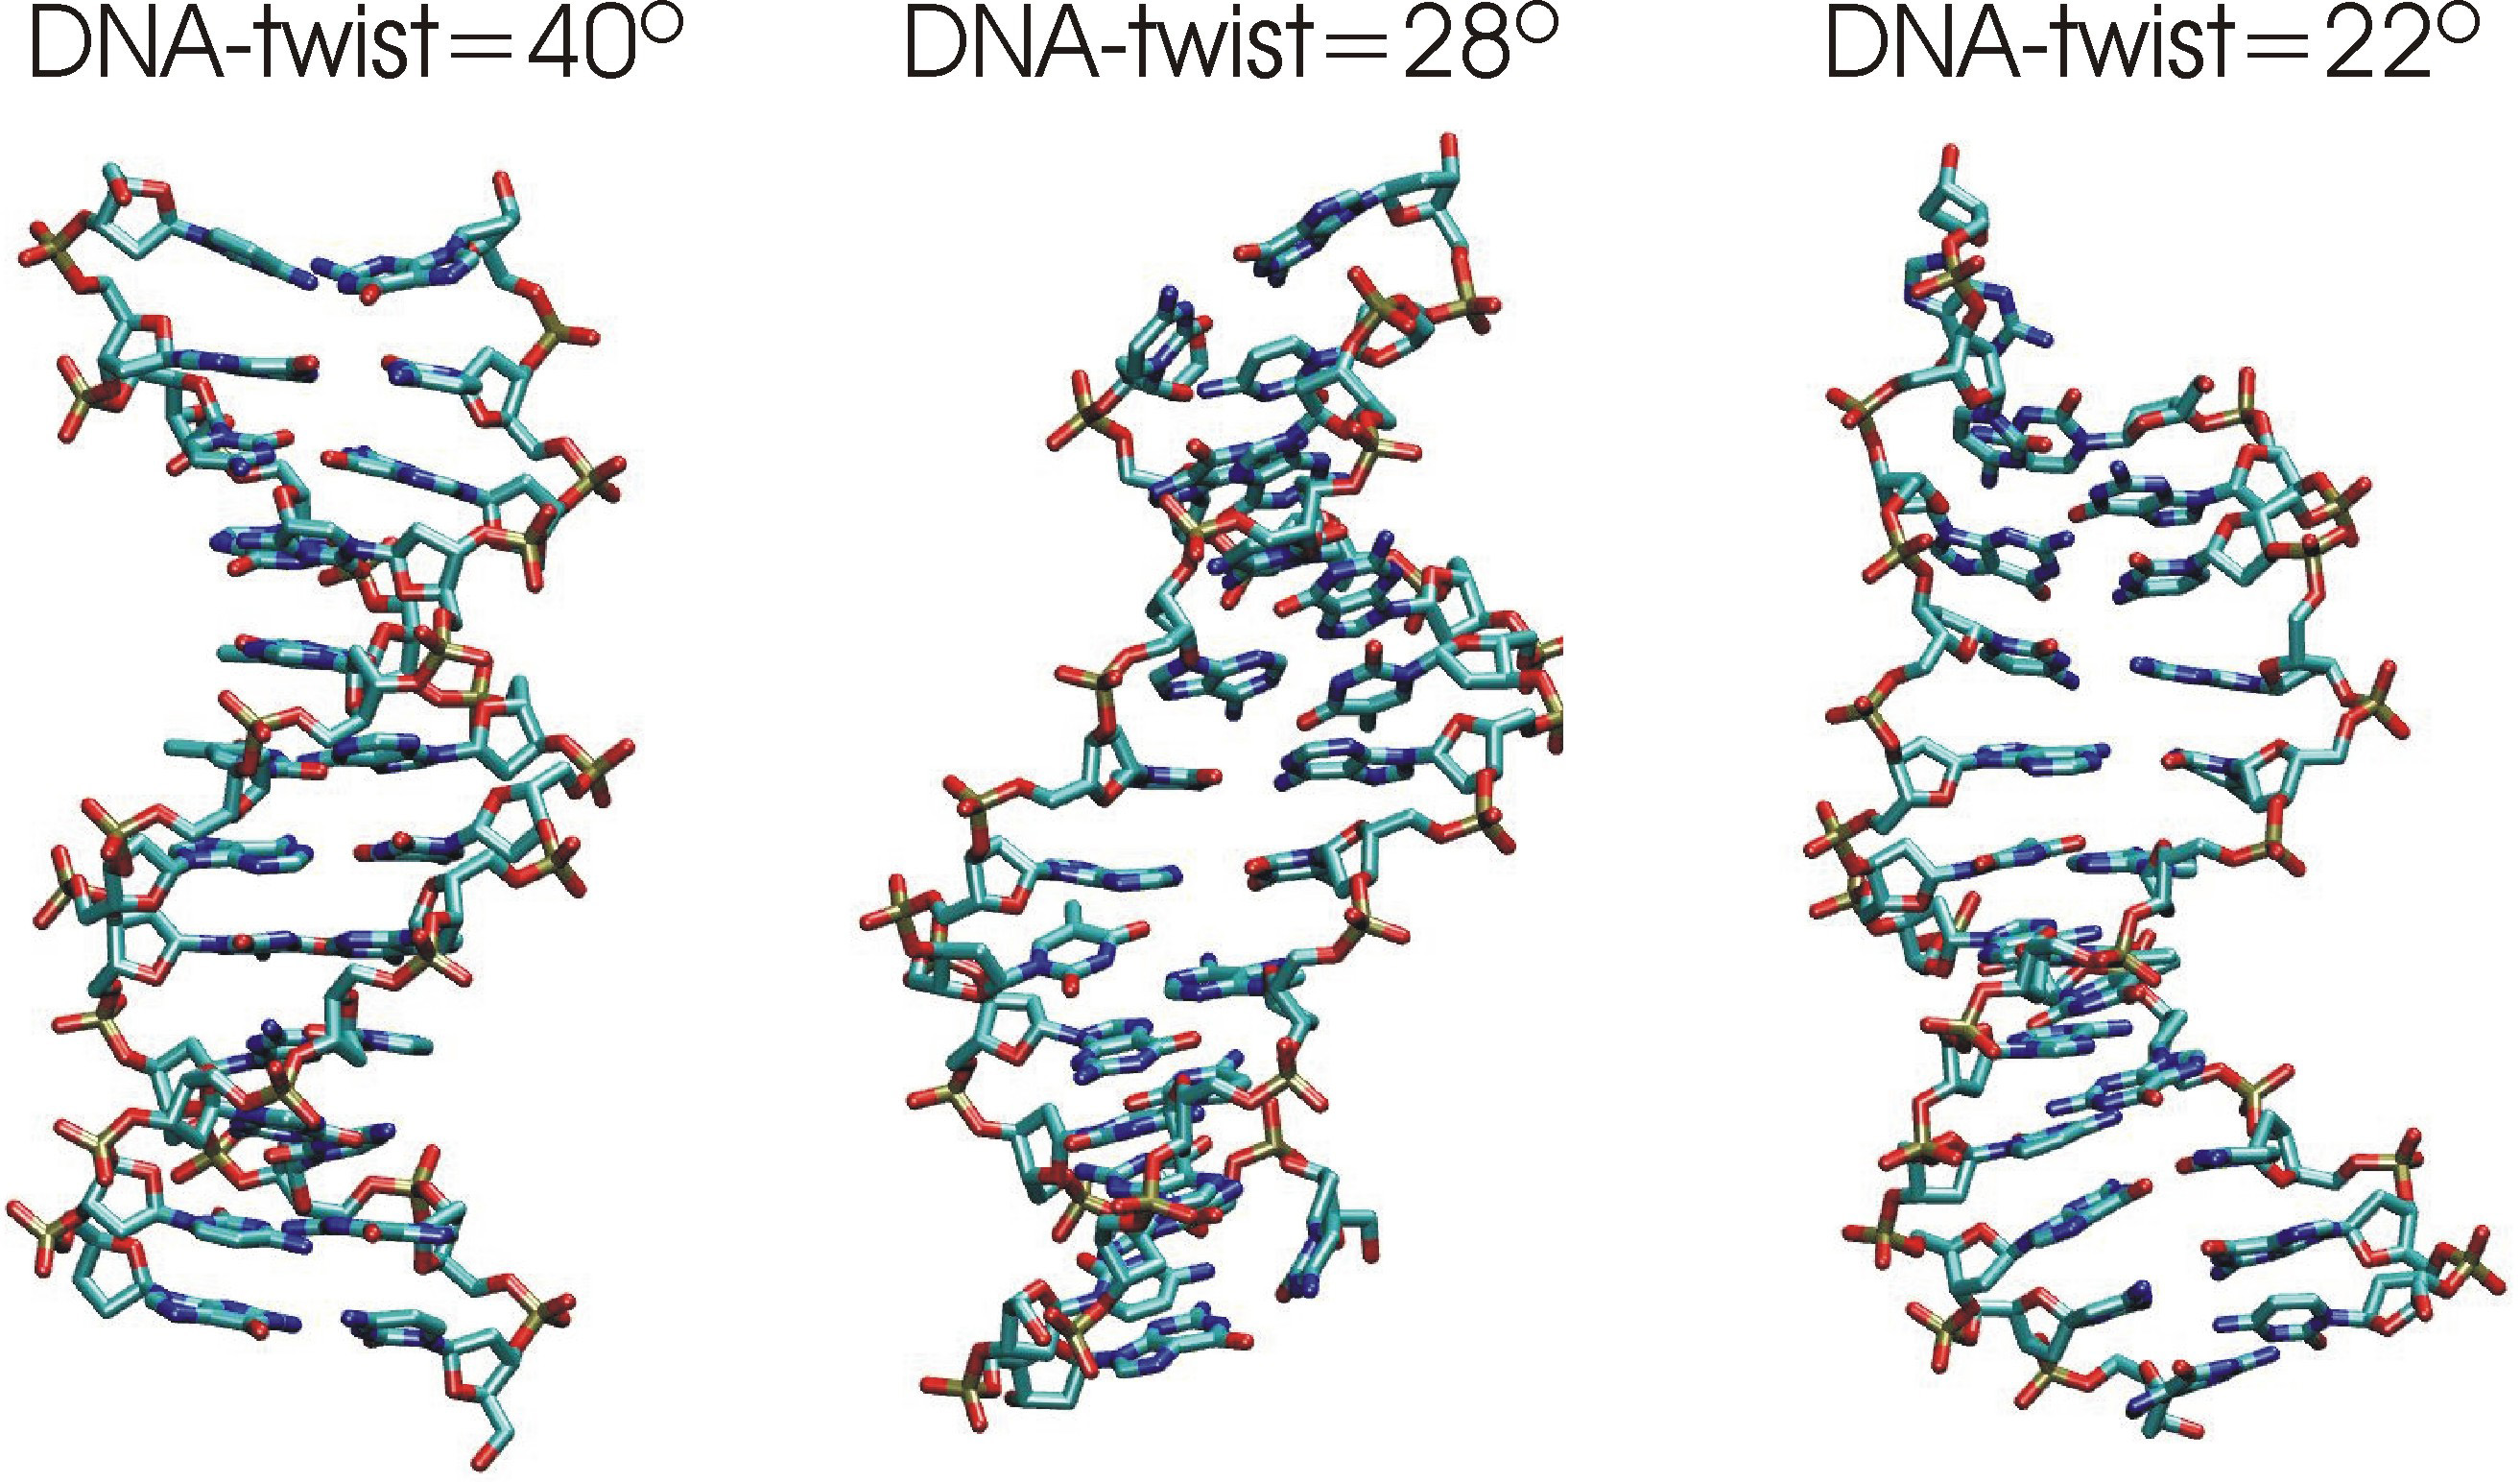
\includegraphics[width=\hsize]{Zacharias/figure_Zacharias_2006.png}
    \mycaption{Overtwisting and untwisting of DNA during molecular dynamics simulations. Explicit solvent molecular dynamics simulations were performed on 12 base pair DNA molecules including a penalty potential for modifying the average DNA twist between 40 degrees (left panel) and 22 degrees (right panel). At twist angles below 25 degrees the DNA splits into a near B-DNA region and a region with average twist of 12 degrees. DNA molecules represent simulation snapshots and are shown as atom color coded stick models. }
       \label{fig:twist}
  \end{center}
\end{figure}

{\sl Flexible Docking of protein-ligand complexes}
\null
Biomolecular association can involve conformational changes of the binding partners. In order to predict the structure of biomolecule complexes using computational docking methods it is necessary to appropriately account for such conformational changes during the simulation. One of our research projects specifically focuses on better accounting for conformational flexibility during docking. A major step that we achieved was the development and testing of a new method to efficiently account for global backbone motions of proteins during protein-protein and protein-ligand docking. In this approach induced fit conformational changes are based on
relaxing the protein conformation in soft collective degrees of freedom of the protein. The flexible global degrees of freedom can be calculated rapidly prior to docking. Very promising results have been achieved on several test systems indicating that this could be a new route for efficient flexible molecular docking. The possibility to use this method to rapidly extract potential drug-like molecules from a data base and identify putative binding sites on protein molecules will be explored in future studies.


\myparagraph{Collaborations}
%
Bremen Area Collaborations:
\begin{enumerate}
\item {\sl International University Bremen}\\Prof. K. Brix \\ Models for Protease Trafficking
\\Prof. F.O. Gl�ckner \\ Sulfatases
\\ Prof. M.-Th. H�tt  \\Topology of protein interaction networks
 \\ Prof. A. Jeltsch  \\ Simulation of enzyme dynamics
\\ Prof. G. Muskhelishvili \\ Molecular modeling
\\Prof. W. Nau\\ Dynamics of end-to-end Contact Formation of Small Peptides
\\Prof. U. Schwaneberg and Dr. D. Roccatano \\Influence of Organic Cosolvents on the Industrially Important Enzyme P450 BM-3
\\Prof. S. Springer\\Conformational Flexibility of MHC Class I Molecules in Ligand-bound and Free States
\end{enumerate}
National \& International Collaborations:
\begin{enumerate}
\item {\sl Technische Universit�t Darmstadt}\\Prof. H.U. G�ringer\\Modeling serum stable RNA aptamers
\item {\sl Institute for Biophysics, Brno, Tschec Rep.}\\Dr. J. Sponer \\Conformational dynamics of RNA
\item {\sl IBPC Paris}\\Dr. C. Prevost\\New Docking Methods
\end{enumerate}
\null
%
\paragraph{Grants}
\begin{enumerate}
\item Funded by DFG, \emph{Protein Protein Docking}, DFG 153/5-1,
(October 2004 - September 2007) \item Funded by DFG, \emph{RNA
Peptid Wechselwirkung}, DFG 153/11-1, (April 2006 - March 2008)
\item Funded by Volkswagenstiftung,  \emph{Replica Exchange},
(January 2005 - December 2007) \item Funded by US Department of
Energy, \emph{US Computational Grande Challenge Project:
Biomolecular Simulation of Base Excision Repair and Protein
Signaling, Pacific Northwest National Laboratory}
\end{enumerate}

\newpage
\paragraph{Other Support Grants}
\begin{enumerate}
\item Cotutelle support grant for PhD student J\'{e}r\'{e}my
Curuksu, Universit\'{e} Franco-Allemande (UFA)
\item Cotutelle support grant for
PhD student Adrian Saladin, Universit\'{e} Franco-Allemande (UFA)
\end{enumerate}

\nocite{Zacharias1,Zacharias2,Zacharias3,Zacharias4,Zacharias5,Zacharias6,Zacharias7,Zacharias8,Zacharias9,Zacharias10,Zacharias11,Zacharias12,Zacharias13,Zacharias14,Zacharias15}

\putbib[combined]
\end{bibunit}

\begin{bibunit}[hplain]
\subsubsection{Computational Systems Biology}
\index{H\"utt, Marc-Thorsten}

\paragraph{Research Team}
%
Marc-Thorsten H\"utt (Professor), Manuel Dehnert (Postdoc), Daniel Geberth (PhD Student), Carsten Marr (PhD Student), Mark M\"uller-Linow (PhD Student), Heike Hameister (Graduate Student), Niko Sonnenschein (Graduate Student) \\

Research of the Computational Systems Biology group focuses on three key topics: biological networks, genome evolution and pattern formation. In essence, we want to understand:
\begin{myitemize}
\item which patterns in gene expression data are related to topological features of the underlying transcriptional regulatory networks;

\item how metabolic fluxes are organized and how patterns of flux redistribution under perturbations come about;

\item how the networks of gene regulation, protein interactions and metabolism interact to organize cellular function;

\item how (statistical) patterns in genome-wide DNA sequences correspond to (or are a consequence of) specific processes of genome evolution;

\item how a measured pattern of cell-cell differences may help predict the precise layout of spatiotemporal structures in \textit{Dictyostelium} self-organization.

\end{myitemize}

In previous years we have particularly established the following methods:

\textit{Biological networks} We have designed a one-parameter class of cellular automata, which can be implemented on arbitrary graphs. With this model system we can quantify the pattern formation capacity of synthetic and real networks.

\textit{Genome evolution} We have shown that patterns in the short-range statistical correlations in DNA sequences serve as an eukaryotic genome signature.  All chromosomes of a species display the same characteristic pattern, markedly different from those of other species.

\textit{Pattern formation} We have shown that in chains of coupled nonlinear oscillators biological variability can induce complex spatiotemporal pattern.


\paragraph{Highlights}
%
The group has moved to IUB in May 2006. It was previously located at
Darmstadt University of Technology. \newline\newline On the level of
research we have achieved the following results in 2006:

\textit{Biological networks} Despite their topological complexity almost all functional properties of metabolic networks can
be derived from steady-state dynamics. Indeed, many theoretical investigations (like flux-balance
analysis) rely on extracting function from steady states. This leads to the interesting question, how
metabolic networks avoid complex dynamics and maintain a steady-state behavior. We exposed
metabolic network topologies to binary dynamics generated by simple local rules. We find that the
network's response is highly specific: Complex dynamics are systematically reduced on metabolic
network topologies compared to networks with similar topologies. Already small topological modifications
substantially enhance the capacity of a network to host complex dynamic behavior and
thus reduce its regularizing potential. This exceptionally pronounced regularization of dynamics
encoded in the topology may explain, why steady-state behavior is ubiquitous in metabolism \cite{MarrEtAl2006}.

We also studied the average excitation density in a simple model of excitable dynamics on graphs and find that this
density is changed
via the distribution pattern of excitations: An increase in connectivity induces a transition from globally to
locally organized excitations and, as a result, leads to an increase in the excitation density. A similar transition
can be induced by increasing the rate of spontaneous excitations while keeping the graph architecture constant \cite{MuellerLinowEtAl2006}.

Furthermore, we looked at the effect of shortcuts on dynamics in regular graphs. It is known that shortcuts in a regular architecture affect the information transport through the system due to the severe decrease in average path length. Our fundamentalnew perspective in terms of pattern formation is the destabilizing effect of topological perturbations by processing distant uncorrelatedinformation, similarly to stochastic noise. We studied this functional coincidence of rewiring and noisy communication on patterns of binary cellular automata \cite{MarrHuett2006}.


\textit{Genome evolution} For the examples of \textit{Mus musculus}
and \textit{Rattus norvegicus} we analyzed in detail short- and intermediate-range statistical correlations in DNA sequences.
These correlation profiles have been computed for all chromosomes of the two species. We find that with increasing
range of correlations the capacity to distinguish between the species on the basis of this correlation profile is
getting better and requires ever shorter sequence segments for obtaining a full species separation. This finding for the first time suggests that distinctive traits within the sequence are situated beyond the level of few nucleotides \cite{DehnertEtAl2006}.

\textit{Pattern formation} This project was started in 2006 and already shows very promising results. We are currently comparing a variety of statistical methods to extract systematic cell-to-cell differences in the case of patterns formed by the slime mould \textit{Dictyostelium discoideum}. We discuss, to what extent these cell properties can serve as predictors of certain later-stage patterns. This work is carried out together with the group of S.C. M�ller (Magdeburg). On the level of modeling, we are investigating how an initial distribution of pacemaker cells is translated by the process of self-organization into a pattern of fully developed spiral waves, represented by a distribution of phase singularities.

On the level of teaching and scientific communication, this year's clear and distinct highlight  for us was to see our new Bioinformatics textbook published by Springer-Verlag \cite{HuettDehnert2006}. Furthermore, a new edited volume on interdisciplinary aspects of self-organization has been published by B\"ohlau-Verlag \cite{VecEtAl2006}. The two-week visit by Professor Larry S. Liebovitch at Jacobs University within the ICTS program in October has helped us reach a new level in our collaboration and write and submit a manuscript summarizing our previous work.


\begin{figure}[ht]
  \begin{center}
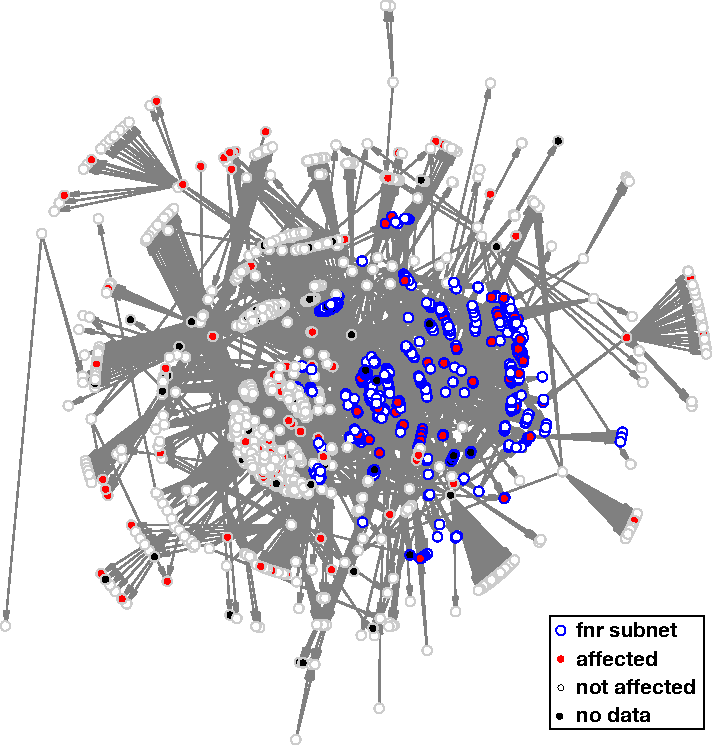
\includegraphics[width=\hsize]{Huett/huett_fig1.pdf}
    \mycaption{ Effect of fnr deletion under anaerobic growth conditions in the largest connected component of the transcriptional regulatory network of \textit{E. coli}. All genes downstream fnr are labeled by a blue circle. We count genes as affected (red disc), when expression levels of wildtype and mutant differ significantly (p value $<$ 0.05). Apparently, the mutation affects many nodes beyond the fnr subnet, indicating that the network compensates for the loss of fnr collectively.}\label{fig:profHuett}
   \end{center}
\end{figure}

\paragraph{Organization}
%
\begin{enumerate}
\item Chair and member of the organizing committee of the British-German Frontiers of Science Meeting 2006 (jointly organized by the Royal Society and the Alexander von Humboldt Foundation)
\item Elected into the Editorial Board of Nonlinear Biomedical Physics (NBP)
\end{enumerate}

\myparagraph{Collaborations}
%
Bremen Area Collaborations:
\begin{enumerate}
\item {\sl International University Bremen} \\ Prof. F.O. Gl�ckner  \\ Genome signatures
 \\Prof. H. Meyer-Ortmanns \\ Discrete and continuous formulations
of excitable dynamics on graphs  \\ Prof. G. Muskhelishvili \\ A
network view on \textit{E. coli} gene expression  \\ Prof. M.
Zacharias \\Topology of protein interaction networks
\end{enumerate}
National \& International Collaborations:
\begin{enumerate}
\item {\sl Florida Atlantic University} \\  Prof. L.S. Liebovitch \\ Transcriptional regulatory network properties in gene expression profiles
\item {\sl Darmstadt University of Applied Sciences} \\  Prof. W.E. Helm \\ Statistical correlations in DNA sequences
\item {\sl Darmstadt University of Technology} \\  Prof. M. Porto \\ Reaction-diffusion processes on scale-free networks
\item {\sl Darmstadt University of Technology} \\ Prof. C. Weihe, Dr. M. M\"uller-Hannemann \\ Impact of motif content on dynamic function of complex networks
\item {\sl Magdeburg University} \\ Prof. S.C. M�ller \\ \textit{Dictyostelium} pattern formation
\item {\sl Max Planck Institute of Molecular Plant Physiology} \\  Dr. W. Weckwerth \\ Consistency of metabolic correlation networks with genome-derived pathway structures
\end{enumerate}


\paragraph{Grants}
\begin{enumerate}
\item Funded by DFG,  \emph{Role of biological variability in the
pattern formation of \textit{Dictyostelium discoideum}, HU-937/4},
(May 2006 - April 2009)
\end{enumerate}

\newpage
\paragraph{Awards, Prizes}
\begin{enumerate}
\item W.E. Heraeus summer school on {\it Statistical Physics of
Gene Regulation: From Genetic Networks to Expression Data and Back
} (organized with H. Meyer-Ortmanns) to take place in July 2007, approved in 2006
\end{enumerate}

\nocite{MarrEtAl2006}

\putbib[combined]
\end{bibunit}

\begin{bibunit}[hplain]
\subsubsection{Statistical Physics of Biological Networks}
\index{Meyer-Ortmanns, Hildegard}

\paragraph{Research Team} Hildegard Meyer-Ortmanns (Professor), Xiang Li (Humboldt Fellow),
Filippo Radicchi (Research Associate), Daniele Vilone
(Postdoctoral Fellow), Sooyeon Yoon (Visiting Graduate Student), Yeong-Yeol Ahn (Visiting Graduate Student)\\

Biological networks are naturally occurring systems of interacting
units. The units are assigned to the nodes such as genes, proteins, metabolites, or neurons,
while regulating relations between the genes or the
proteins, chemical reactions between metabolites, or
synaptic connections between the neurons are assigned to the edges of
the network. A number of models is used to describe various
dynamical aspects. One of these models are Boolean networks that were introduced
by Stuart Kauffman in 1969 as a simple model for genetic systems.\\
A topical issue in the context of genetic networks is an
explanation of the low number of stable cell states in spite of the fact that
many states are in principle possible if all combinations of
genes would be allowed. Boolean dynamics may result in a limited
number of attractors in phase space and - if attractors actually represent cell states- Boolean
dynamics would explain
the observation of a few stable cell states. Random Boolean networks are directed
graphs with $N$ nodes each of which takes a Boolean value $0$ or $1$.
Usually the nodes are synchronously updated from time $t$ to time
$t+1$ according to coupling functions that are chosen randomly
from a certain set of Boolean functions. As it turned out, the
increase of the number of stable attractors as a function of the
system size does depend on the updating mode, being
synchronous or asynchronous. An exponential growth of the
number of attractors with the system size seems to be an artifact of the
synchronous update which is not realistic from the biological
point of view.

\paragraph{Highlights}
%
\textit{Synchronous versus asynchronous update}
We have started with a systematic study of synchronous versus
asynchronous updating modes, first applied to an Ising chain in
which each unit can take only two possible values, $+1$ or $-1$.
Already in this simple system we observe a phase transition
between the stationary states of the time evolution
\cite{meyerortmanns1} if we interpolate between synchronous and
asynchronous updating. (Interestingly for physicists: this
transition belongs to the universality class of parity
conservation.) In general, the effect of such a transition may be
that in one of these phases the stationary states have lost any
remnants to the intrinsic dynamics that was imposed on the
individual nodes of the network. In this case the stationary
states are no longer representative for a certain intrinsic
dynamics, but depend on the time-order of updating events.
In turn this has an impact on the interpretation of datasets
as reflecting certain intrinsic dynamics.\\

\begin{figure}[ht]
  \begin{center}
    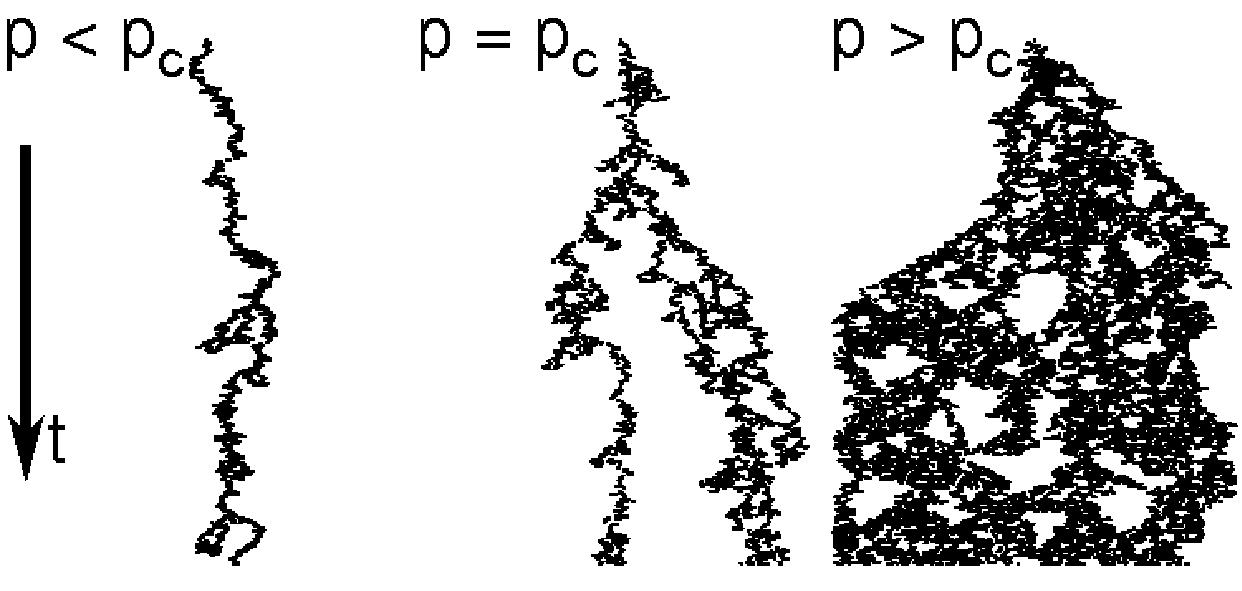
\includegraphics[width=\hsize]{Meyer-Ortmanns/meyerortmanns.pdf}
    \mycaption{Directed percolation process in time as it also occurs for processes of epidemic spreading.
$p_c$ is a critical parameter beyond which the qualitative behavior changes.}\label{fig:meyerortmanns1}
   \end{center}
\end{figure}

We will generalize the dynamics and vary the updating rules to
biologically more relevant ones. In this way we can check which
features of the space of attractors depend on the used procedures
and how the number of stable cell states is influenced by the
order of updating events. \newline \newline Hildegard Meyer-Ortmanns is also involved in ``Statistical Physics: Dynamical Processes on Complex
Networks''.


\paragraph{Organization}
\begin{enumerate}
\item  ICTS-seminars 2006
\end{enumerate}

\myparagraph{Collaborations}
%
Bremen Area Collaborations:
\begin{enumerate}
\item {\sl International University Bremen}\\Prof. M.-Th. H\"utt\\Genetic Networks
\\Prof. C. Hilgetag\\Neural Networks
\item {\sl Bremen University} \\Prof. S. Bornholdt\\Boolean Networks
\end{enumerate}

National \& International Collaborations:
\begin{enumerate}
\item {\sl Kyung Hee University, Seoul (Korea)}\\ Prof. S.-H.
Yook\\ Percolation theory and epidemic spreading
\item{\sl Korea Institute of Advanced Science and Technology, Daejeon,
Korea}\\Y.Y. Ahn\\ Neural Network Models for the Visual
Cortex of the Monkey
\item{\sl Humboldt University Berlin}\\Prof. M. Zaks\\ Dynamics of Excitable Media
\item {\sl Technische Universit\"at Hamburg Harburg}\\ Prof. A.-P. Zeng\\ Autocatalytic Sets and Metabolic Networks
\end{enumerate}


\paragraph{Grants}
\begin{enumerate}
\item Funded by DFG,  \emph{Hierarchische Netzwerke}, ME
1332/10-2, (April 2004 - March 2007)
\end{enumerate}

\paragraph{Other Support Grants}
\begin{enumerate}
\item Humboldt-Stiftung, Fellowship, Humboldt-Stiftung
IV-CHN/1116658 STP
\item 2 DAAD-grants (Germany-Korea): a) ``Physics of Surface Growth'', b) ``Neural Networks''
\end{enumerate}


\paragraph{Awards, Prizes}
\begin{enumerate}
\item W.E. Heraeus summer school on {\it Interfaces between Physics
and Computer Science} to take place in June 2007, approved in 2006
\item W.E. Heraeus summer school on {\it Statistical Physics of
Gene Regulation: From Genetic Networks to Expression Data and Back
} (organized with M.T. H\"utt) to take place in July 2007, approved
in 2006
\end{enumerate}

\nocite{ortmanns0M}
\nocite{ortmanns1M}
\nocite{ortmanns2M}
\nocite{ortmanns3M}
\nocite{ortmanns4M}
\nocite{ortmanns5M}
\nocite{ortmanns6M}
%\nocite{meyerortmanns1M}
\nocite{vilone1M}

\putbib[combined]
\end{bibunit}


\newpage \shorttitle{Biophysics}
\subsection{Biophysics}

The Biophysics section at Jacobs University Bremen is a very good example of modeling and experiment joining forces in an attempt to understand the link between structure and function of biomolecules. The objects of interest are membrane proteins involved in antibiotics transport, which place this endeavor well within the target areas of research at Jacobs.\\

Highlights of 2006 in the Biophysics section include a Summer School on biosensing and a deeper understanding of the passage of antibiotics through the membrane channel.\\


\begin{bibunit}[hplain]
\subsubsection{Membrane Transport}
\index{Winterhalter, Mathias}

\paragraph{Research Team}
%
Mathias Winterhalter (Professor), Yannic Ramaye (Postdoc), Helge
Weingart (Postdoc, Project Manager), Tivadar Mach (PhD Student), Joana
Gomes (PhD Student), Raghavendra Palankar (PhD Student), Que Tien Tran
(PhD Student), Stefanie T�mmers (PhD Student)\\

The outer cell wall of \textit{Escherichia coli} contains a number of channel forming
proteins called porins. Such channels allow e.g. bacteria to harvest nutrients.
Our main research focus is on the characterisation of transport across such
membrane channels. For this our method of choice is to reconstitute
membrane channels into planar lipid bilayers and characterise them by time
resolved ion current. For example, previously we have been able to follow the
translocation of single sugar molecules through Maltoporin. Maltose
molecules diffusing into the channel will create typical fluctuations in ion
conductance. An analysis of this ``noise in the ion current'' allows to conclude
on the mode of translocation and the underlying molecular interaction. For
example, we quantified the highly selective and efficient transport for maltose
harvesting from the outside to the inside. How sophisticated nature had
designed this uptake pathway is seen in the asymmetry of the transport: its
four times faster than in the opposite direction.



\paragraph{Highlights}
%
A related question is to understand the pathway of antibiotics. For example
OmpF, is a general diffusion porin allowing smaller molecules to permeate and
is known to facilitate the translocation of antibiotics like Ampicillin.
Within our EU-research network we characterised the
transport of a series of penicilins. Measuring the ion current fluctuation in
presence of different concentrations of penicilins revealed a clear correlation
between permeation and biological activity. The data serves as an input for
the group of M. Cecarelli (University of Sardenia, Cagliari) to perform one of
the most powerful nonequilibrium molecular dynamic simulations to elucidate
the effect of molecular interaction during transport. Together with Prof. P.
Gameiro we quantified the translocation of a recently developed new class of
antibiotics fluroquinilones. We found a high translocation number of the
hydrophilic ones whereas the more hydrophobic ones might also permeate
through the outer membrane without channels. In collaboration with
Dr. Claus F�tterer (Institut Curie), Dr. Niels Fertig (Nanion) and our
colleague Dr. J�rgen Fritz (Jacobs University) we miniaturize our set-up using microfluidics.
This reduced now the required volume from mili- to a few microliter. In collaboration
with Dr. U. Kleinekath�fer we measured the temperature dependence of the
conductance and compared the results with molecular modelling.

\begin{figure}[ht]
  \begin{center}
   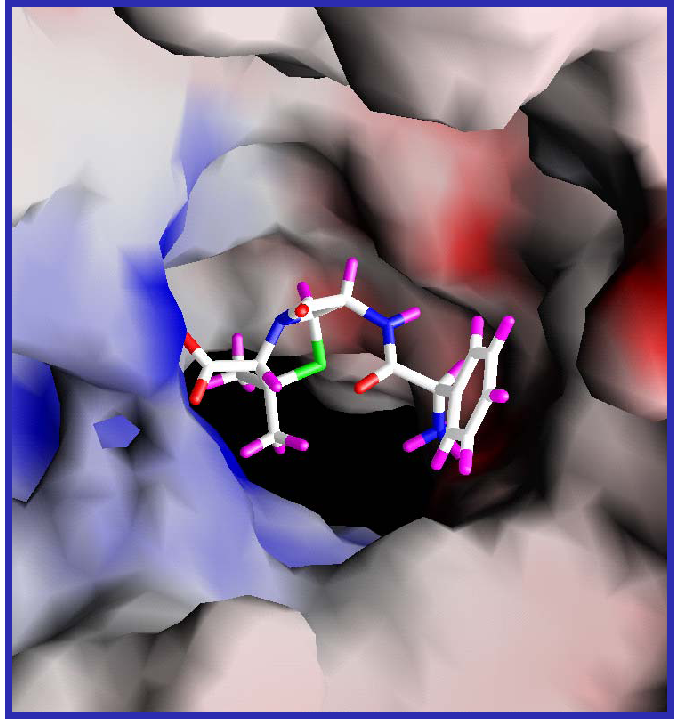
\includegraphics[width=\hsize]{Winterhalter/Winterhalter_fig1.pdf}
    \mycaption{Molecular modelling revealed a binding site for Ampicillin inside an OmpF channel.}
    \label{fig1:Winterhalter}
  \end{center}
\end{figure}

In collaboration with Dr. S.M. Bezrukov (National Institutes of Health, Bethesda,
 USA) we could resolve a single lambda phage binding to its receptor maltoporin.\newline \newline Mathias Winterhalter is also involved in ``Nanocapsules''.
%
% to reference it use ``Figure.~\ref{fig:xxx}''; the numbers will be computed automatically.

% to include a figure, generate a file xxx.pdf and integrate the following lines
%\begin{figure}[ht]
%  \begin{center}
%    \includegraphics[width=6cm]{fig2.pdf}
%    \caption{Typical tracks of ion currents through single trimeric OmpF channels reconstituted into planar lipid membranes at the presence of zwitterionic and anionic penicillins. Membrane bathing solutions contained 1M NaCl (pH 5.0), 5.7 mM of indicated antibiotic, and the applied voltage was -100 mV.  Time resolution was 0.015 msec. (A) Penetrating zwitterionic (ampicillin or amoxicillin) amino penicillins modulate ion current through OmpF.  In the absence of antibiotic (left) the ion current is mainly determined by the geometry and surface properties of the channel pore.  The current is stable; no high-amplitude interruptions are seen.  In the presence of 5.7 mM ampicillin (middle) or amoxicillin (right), one of the three OmpF pores gets spontaneously blocked by a translocating drug molecule.  At high time resolution these blockages are seen as well defined steps to 2/3 of the open channel current and back.  (B) Anionic penicillins do not significantly affect ion current through OmpF.  No interruptions in the current can be seen in the presence of piperacillin (left), azlocillin (middle) or carbenicillin (right).}
%    \label{fig2:Winterhalter}
%  \end{center}
%\end{figure}

\paragraph{Organization}
\begin{enumerate}
\item  We organized a summerschool on Biosensing: Faster smaller, smarter shop at International University
(28.7.-4.8.) with more than 100 participations from 12 countries. A second summerschool on Complex
Materials from June 24th to July 1st. This summerschool included lectures and practical
courses for about 50 participants in the field.
\end{enumerate}



\myparagraph{Collaborations}
%
Bremen Area Collaborations:
\begin{enumerate}
\item {\sl International University Bremen} \\ Prof. J. Fritz \\ Microfluidics for electrophysiology and liposome separation
 \\ Prof. U. Kleinekath�fer \\ Ion and antibiotics transport
through membrane proteins  \\ Prof. S. Springer \\ Injection of
engineered nanocapsules into cells for use as sensors  \\ Prof. M.
Ullrich \\ Multidrug Efflux pumps
\item {\sl Universit�t Bremen, Chemie} \\ Prof. D. Gabel \\ Liposome as carriers
\item {\sl Hochschule Bremen} \\ Prof. V. Hass \\ Process control
\end{enumerate}
National \& International Collaborations:
\begin{enumerate}
\item {\sl University of W�rzburg} \\Prof.  R. Benz \\ Porin
\item {\sl NIH, Bethesda}\\ Dr. S.M. Bezrukov \\ Single molecule transport
\item {\sl MPI Berlin} \\ Prof.  G.B. Sukhorukov \\ Functional
nanocapsules
\item {\sl University of Toulouse} \\ Prof.  D. Fournier \\ Functional
nanocapsules
\item {\sl University of Toulouse}\\ Prof.  P. Faller \\ Microcalorimetry
\item {\sl University of Porto} \\ Prof.  P. Gameiro \\ Antibiotic
translocation
\item {\sl University of Syrakuse} \\ Prof.  L. Movileanu \\ OmpF
characterisation
\item {\sl University of Copenhagen}\\ Prof.  T. Heimburg \\ Lipip phase
transition\end{enumerate}

\paragraph{Grants}
\begin{enumerate}
\item Funded by EU, Training network \emph{Molecular origin of
antibiotic translocation}. This project is performed in
collaboration with N. Fertig (M�nchen), H. Vogel (Lausanne), J.M.
Pages (Marseille), P. Gameiro (Porto), M. Page (Basel), PI M.
Winterhalter.,  (January 2006 - December 2006)

\item Funded by Volkswagen Stiftung,  \emph{Complex Materials:
Cooperative Projects of the Natural, Engineering, and Biosciences:
Nanoengineered polymer capsules: Detection and manipulation for
nanoreactors and controlled delivery.} (I/80 051) in collaboration
with G. B. Sukhorukov (coordinator, MPI Potsdam), A. L. Rogach
(LMU Munich) and W. J. Parak (LMU Munich), (October 2004 -
September 2007)

\end{enumerate}

\paragraph{Other Support Grants}
\begin{enumerate}
\item Volkwagen Stiftung ``Summerschool on Complex Materials'':
\item Eureka 3271 Nano to Bio (PI L. Levy, Nanobiotix, Paris; J.F. Hochepied, Ecole des Mines, Paris)

\item German-french University: Summerschool on Biosening, faster, smaller, smarter.

\item DAAD Exchange program with Porto
\end{enumerate}

\nocite{Winterhalter1,Winterhalter2,Winterhalter3,Winterhalter4,Winterhalter5,Winterhalter6,Winterhalter7,Winterhalter8,Winterhalter9,Winterhalter10,Winterhalter11,Winterhalter12}

\putbib[combined]
\end{bibunit}

\begin{bibunit}[hplain]
\newpage
\subsubsection{Modeling of Transport Channels}
\index{Kleinekath\"ofer, Ulrich} \label{Bio:Kleinekathoefer}

\paragraph{Research Team}
Ulrich Kleinekath\"ofer (Professor), GuanQi Li (PhD Student), J\"org Liebers
(Diploma Student, still TU Chemnitz), Carsten Olbrich
(PhD Student), Soroosh
Pezeshki (PhD Student), Markus Schr\"oder (PhD Student)\\


The research of our computational physics group in the direction of
biological systems is twofold: large scale classical molecular dynamics
simulations on one hand and quantum dynamical calculations for electron and
excitation transfer processes on the other. In the study of some systems
these different approaches are used separately and jointly in others.  The
ion and antibiotics transport through the outer membrane protein F (OmpF)
and the large domain motion within the molecular motor ATPase are, so far,
simulated using purely classical molecular dynamics simulations.  Quantum
dynamical studies are used to investigate e.g. electron transfer within
DNA.  Combinations of classical and quantum mechanical methods are used to
study the light-harvesting in purple bacteria. To perform an atomic level
description of the light-harvesting process classical molecular simulations
are complemented with quantum chemistry calculations and quantum modelling.



\paragraph{Highlights}
%
\emph{Ion transport} The study of transport through the membrane protein
OmpF was triggered by the ongoing experiments in the group of Prof.
Winterhalter at Jacobs University. It is known that the transports of antibiotics through
the outer membrane of bacteria takes place via the membrane protein OmpF.
Once the antibiotics passed the outer membrane of bacteria they are able to
fulfill there task, i.e. destroy the bacterium. Since resistance against
known antibiotics is an increasing problem, new antibiotics have to be
developed and these antibiotics have to be able to quickly pass the OmpF.
To study the passage of antibiotics through the membrane channel the
Winterhalter group measures the ion conductance and its blockage for
different antibiotics.


\begin{figure}[ht]
  \begin{center}
   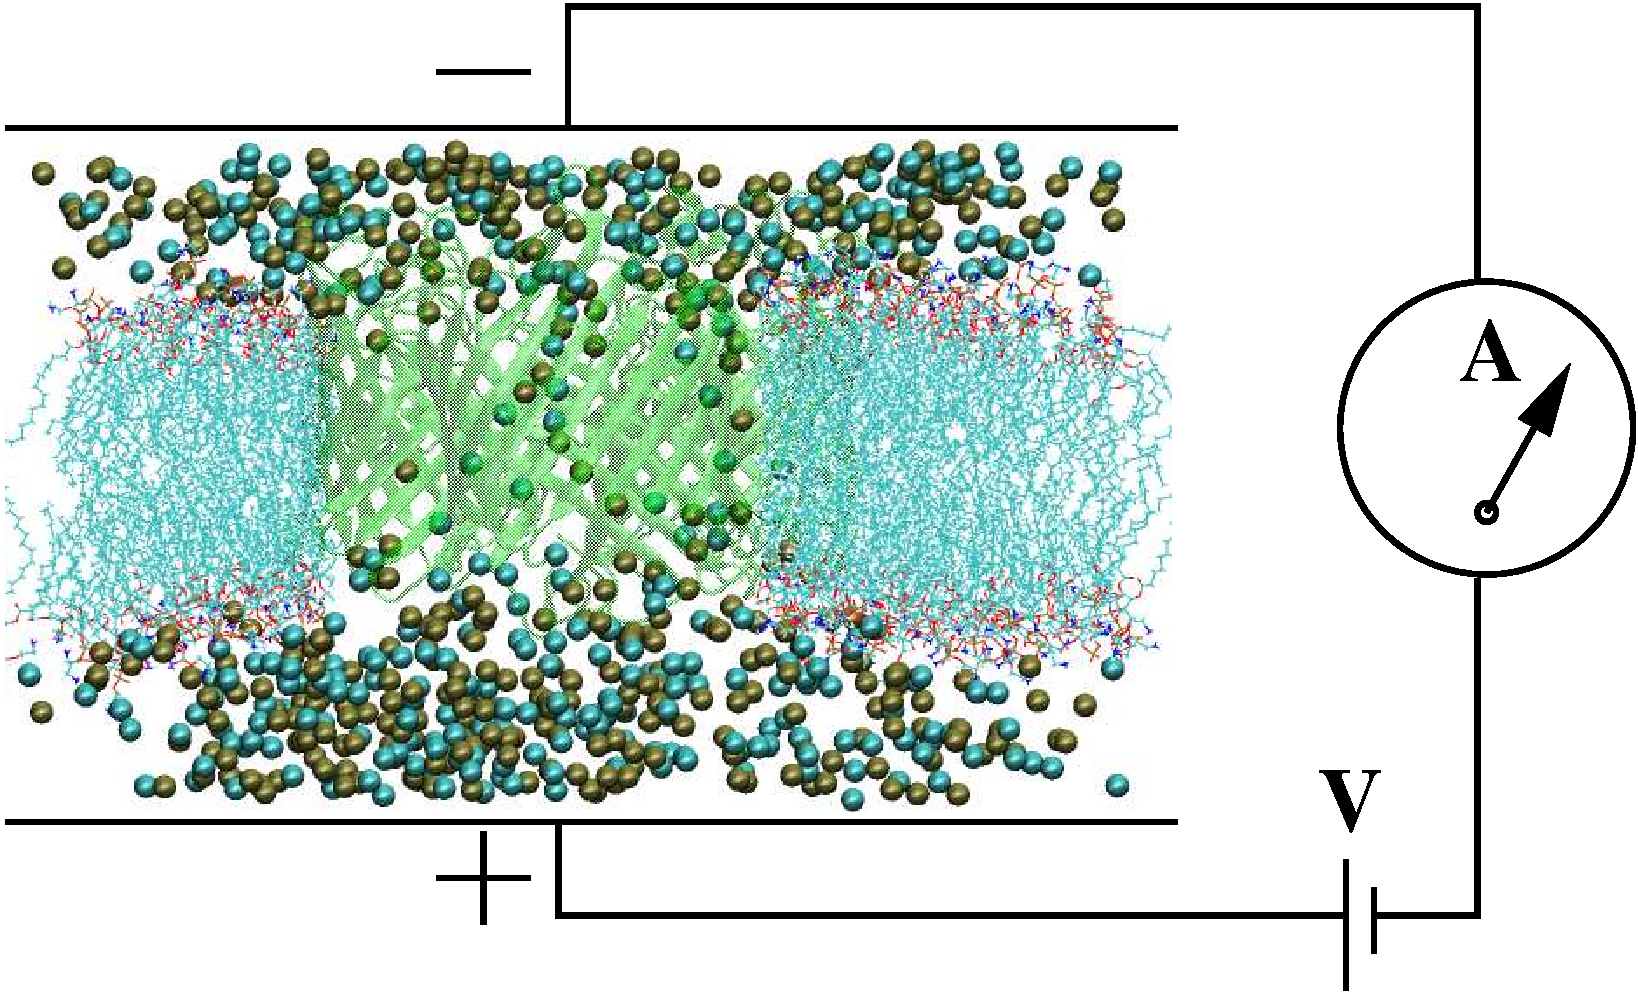
\includegraphics[width=\hsize]{Kleinekathoefer/kleinekathoefer_fig1.pdf}
    \mycaption{Sketch of the ion transport simulations through the OmpF
      protein. A trans-membrane potential is applied to the simulation
      cell.} \label{fig:profkleinekathoefer1}
   \end{center}
\end{figure}

For the simulation and detailed explanation of these experiments a
splitting into two sub-problems is possible: first the determination of the
ion current through the OmpF protein without antibiotics and then in a
second step a steering of the antibiotics through the pore. Within
large-scale molecular dynamics simulation involving about 90 000 atoms a
transmembrane potential is applied. To gain a reasonable statistics the
simulation time needs to be at least 10 ns (1 ns $\approx$ 1 day on 30
2GHz-Opteron-CPUs). Depending on the applied voltage only very few charge
carriers do cross the membrane within 1ns simulation time. Nevertheless the
calculated current and conductivities do correspond rather nicely to the
measured values. Especially the temperature dependence of the ion
conductivity show a similar behavior in experiment and simulations.
First simulations steering substances through the pore also have been
performed. Due to problems with the antibiotics force fields, these test
run had to be done using nucleic acids and sugars. Force fields for
antibiotics are being under development.


\emph{Light-harvesting systems} For an ensemble of B850 rings of the
light-harvesting system LH2 of purple bacteria the linear absorption
spectrum was calculated. Using different Markovian and non-Markovian,
time-dependent and time-independent methods based on second-order
perturbation theory in the coupling between the excitonic system and its
surrounding environment, the influence of the shape of the spectral density
on the linear absorption spectrum was demonstrated for single samples and
in the ensemble average.  For long bath correlation times non-Markovian
effects clearly show up in the static absorption line shapes. Among the
different spectral densities studied was one of the bacterium
\emph{Rhodospirillum (Rs.) molischianum} obtained from molecular dynamics
simulations.  The effect of static disorder on its line shapes in the
ensemble average was analyzed and the results of the present calculations
were compared to experimental data.  \newline \newline Ulrich
Kleinekath\"ofer is also involved in ``Molecular Electronics and Dynamics''.

\myparagraph{Collaborations}
%
Bremen Area Collaborations:
\begin{enumerate}
\item {\sl International University Bremen} \\ Prof. M. Winterhalter
  \\ Ion and antibiotics transport through membrane proteins
  \end{enumerate}
National \& International Collaborations:
\begin{enumerate}
\item {\sl Universit\`a degli Studi di Cagliari} \\ Prof. P. Ruggerone,
  Prof.\ M. Cecarelli
  \\ Transport through membrane proteins
\item {\sl Beckman Institute, University of Illinois at Urbana-Champaign}
  \\ Prof.\ K. Schulten,  B. Isralewitz, PhD
\\ Simulation of a $\beta$-subunit of ATPase
\item {\sl Pittsburgh Supercomputing Center}
  \\ M. Dittrich, PhD \\ Simulation of a $\beta$-subunit of ATPase
\end{enumerate}



\paragraph{Grants}
\begin{enumerate}
\item Funded by DFG, \emph{light-harvesting complexes}, KL
  1299/3-1 (October 2006 - September 2008)
\item Funded by DFG, priority program SPP 1243 \emph{Quantum transport
  at the molecular scale}, KL 1299/4-1 (November 2006 - December
  2008)
\end{enumerate}
\newpage

\nocite{profkleinekathoeferwela05a}
\nocite{profkleinekathoeferschr05a}
\nocite{profkleinekathoeferwela05b}
\nocite{profkleinekathoeferklei06a}
\nocite{profkleinekathoeferklei06b}
\nocite{profkleinekathoeferklei06c}

\putbib[combined]
\end{bibunit}


\shorttitle{Biotechnology}
\subsection{Biotechnology}

While within the Biophysics section, research attempts to understand the relation between protein structure and function and the Computational Biology studies place structural data into a systemic context, research in the Biotechnology section is about the \textit{design} of function.\\

Here the research activities range from enzyme design and directed protein evolution to large-scale screening for functional properties and molecular modeling as a route towards bioengineering.\\

In this form Biotechnology research at International University Bremen successfully addresses target areas ranging from energy and materials to water and food, as well as health. The wide variety of 2006 highlights demonstrate impressively the impact Biotechnology research at Jacobs already has on these target areas. These highlights include intense and successful joint projects with industry, several patents, substantial progress in carrying gene silencing technology to human cell lines and proofs of principle to several biotechnological and bioengineering concepts.\\


\begin{bibunit}[hplain]
\subsubsection{Enzyme Design}
\index{Jeltsch, Albert}

\paragraph{Research Team}
%
Albert Jeltsch (Professor),
Sandra Becker (Technician),
Sanjay Chahar (PhD Student),
Arunkumar Dhayalan (PhD Student),
Renata Jurkowska (PhD Student),
Tomek Jurkowski (PhD Student),
Heike Laser (Postdoc),
Kirsten Liebert (Postdoc),
Sergei Ragozin (Postdoc),
Philipp Rathert (PhD Student),
Christian Rohde (PhD Student),
Martina Schlickenrieder (PhD Student),
Maike Schwerdtfeger (Lab Technician),
Yinying Zhang (PhD Student)\\

%Albert Jeltsch, Prof. Dr., Prof. of Biochemistry,
%Sandra Becker, Technician,
%Sanjay Chahar, M.Sc., PhD student,
%Arunkumar Dhayalan, M.Sc., PhD student,
%Renata Jurkowska, M.Sc., PhD student,
%Tomek Jurkowski, M.Sc., PhD student,
%Heike Laser, Dr., PostDoc,
%Kirsten Liebert, Dr., PostDoc,
%Sergei Ragozin, Dr., PostDoc,
%Philipp Rathert, Dipl. Biol., PhD student,
%Christian Rohde, Dipl. Biol., PhD student,
%Martina Schlickenrieder, Dipl. Biol., PhD student,
%Maike Schwerdtfeger, Technician,
%Yinying Zhang, M.Sc., PhD student\\

The research of my group in the field of Biotechnology and protein design focuses on the following projects: i) We aim to design DNA methyltransferases that can be employed for targeted methylation of the human genome. This approach could lead to a novel approach to shutdown the expression of genes in vivo which could have a wide range of applications in the future including treatment of cancer and viral infections. ii) We apply methods of directed and evolutionary protein design to generate DNA methyltransferase with improved properties for various applications.  iii) Based on our expertise in protein design and directed evolution approaches we develop general method for biotechnological applications.

\paragraph{Highlights}
%
Gene silencing by targeted DNA methylation has potential applications in basic research and therapy. To establish targeted methylation in human cell lines, the catalytic domains of mouse Dnmt3a and Dnmt3b DNA methyltransferases (MTase) were fused to different DNA binding domains of GAL4 and an engineered zinc finger domain. In collaboration with M. Papworth (Cambridge, UK) and F. Li (Shanxi, China) we demonstrated that
\begin{enumerate}
\item { Dense DNA methylation can be targeted to specific regions in gene promoters using chimeric methyltransferases.}
\item { Site-specific methylation leads to repression of genes controlled by various cellular or viral promoters.}
\item { Mutations affecting any of the DNA binding domains, MTase or target DNA sequences reduce targeted methylation and gene silencing.}
\item { Targeted DNA methylation is effective in repressing HSV-1 infection in cell culture with the viral titer reduced by at least 18-fold in the presence of an MTase fused to an engineered zinc finger DBD, which binds a single site in the promoter of HSV-1 gene IE175k.}
\end{enumerate}
Our results demonstrate that it is possible to direct DNA methyltransferase activity to predetermined sites in DNA, achieve targeted gene silencing in mammalian cell lines and interfere with HSV-1 propagation.

\begin{figure}[ht]
  \begin{center}
   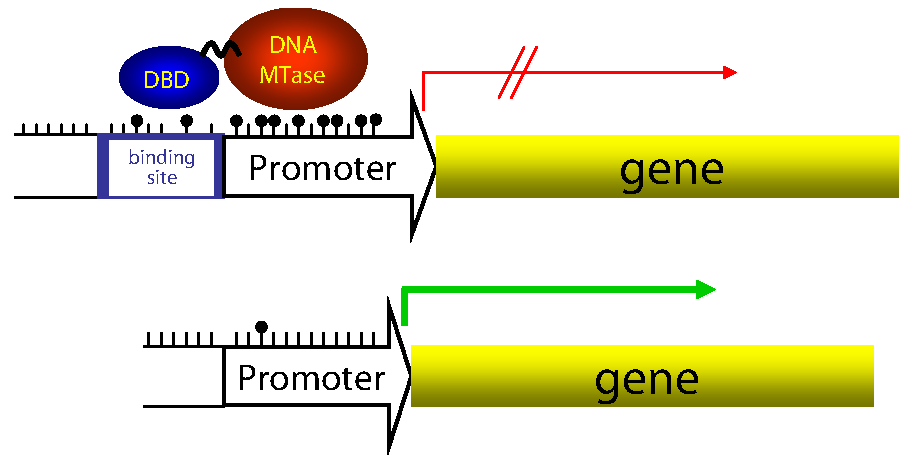
\includegraphics[width=\hsize]{Jeltsch/Fig_Jeltsch2_2006.pdf}
    \mycaption{Schematic drawing of the specific methlytion of DNA by DNA binding domain-DNA MTase fusion proteins.}\label{Fig_Jeltsch2_2006.pdf}
   \end{center}
\end{figure}


Protein/protein interaction is an essential process in cellular physiology. In addition, protein/protein interaction sites are potentially important drug targets, because manipulation of protein/protein interaction will allow for a specific interfer-ence will cellular metabolism and regulation. Therefore, mapping of the interfaces of protein complexes is an important task. We have developed a general system that allows us to deine the residues involved in protein/protein interaction for any pair of proteins. In the first step a yeast-two hybrid construct is prepared for the pair of proteins to be analyzed. Such systems are already established for many protein pairs due to various high-throughput projects aiming to identify protein/protein interaction. In the next step, one of the two partners is subjected to high-level randomization and the library selected for clones that still do interact. These clones are sequenced. Since the amino acid exchanges observed in such clones did not interfere with protein/protein interaction, they will provide a negative footprint of the interaction region, where mutations are excluded. This method may be useful for large scale high throughput mapping of protein/protein interaction sites.\newline \newline Albert Jeltsch is also involved in ``Biochemistry - Methyltransferases''.


\myparagraph{Collaborations}
%
Bremen Area Collaborations:
\begin{enumerate}
%
\item {\sl International University Bremen} \\ Prof. K. Brix \\ Confocal cell imaging
 \\ Prof. G. Mushkelishvili \\ AFM of DNA methyltransferases
 \\ Prof. W. Nau \\ Investigation of Peptide Dynamics
\\ Prof. S. Springer \\ Rapid Kinetics
\\ Dr. H. Stamerjohanns \\ Data analysis and web programming
 \\ Prof. M. Ullrich \\ Mass spectrometry
 \\ Dr. C. Voelcker-Rehage \\ Genkotyping participants of the JC aging study
 \\ Prof. M. Winterhalter \\ Dynamic light scattering
 \\ Prof. M. Zacharias \\ Simulation of enzyme dynamics
\end{enumerate}
National \& International Collaborations:
\begin{enumerate}
\item {\sl University of Texas, Department of Carcinogenesis, Smithville, Texas, USA} \\ Prof. M.T. Bedford \\ Peptide interaction of DNA methyltransferases
\item {\sl Emory University Atlanta, Department of Medicine, GA, USA} \\ Prof. X. Cheng \\ X-ray crystallography and inhibitor design of DNA methyltransferases
\item {\sl Universit�t Halle} \\ Prof. R. Dammann \\ Expression of Dnmt1 in cells
\item {\sl University of Edinburgh, Edinburgh, UK} \\ Prof. D.T.F. Dryden \\ Time resolved fluorescence spectroscopy with DNA methyltransferases
\item {\sl Laboratory of Cancer Epigenetics, Faculty of Medicine, Free University of Brussels, Brussels, Belgium} \\ Prof. F. Fuks \\Phosphorylation of DNA methyltransferases
\item {\sl DKFZ, Heidelberg} \\ Prof. I. Grummt \\ Regulation of DNA methyltransferases in cells
\item {\sl Hungarian Academy of Science, Szeged, HU} \\ Prof.  A. Kiss \\ Expression and Design of the M.SssI DNA methyltransferase
\item {\sl Department of Biochemistry and Molecular Biology, University of Shaanxi, China} \\ Dr. F. Li \\Targeted methylation of DNA in cells
\item {\sl DKFZ, Heidelberg} \\ Dr. F. Lyko \\ Expression and characterisation of Dnmt2
\item {\sl University of Groningen, Groningen, The Netherlands} \\ Dr. P. McLaughlin\\ Targeted methylation of DNA in cells
\item {\sl National Cancer Institute, Frederick, MD, USA} \\ Prof. K. Muegge \\ Regulation of Dnmt3a in cells
\item {\sl Institut f�r Genetik, Universit�t Kassel} \\Prof. W. Nellen \\ Expression and characterisation of Dnmt2
\item {\sl The Wellcome Trust Biocentre, University of Dundee, Dundee, UK} \\ Prof. T. Owen-Hughes \\ Preparation of nucleosomal DNA
\item {\sl MRC, Cambridge, UK} \\ Dr. M. Papworth\\ Targeted methylation of DNA in cells
\item {\sl Leibnitz Institute for Age Research, Jena} \\ Dr. M. Platzer \\ High troughput DNA Sequencing
\item {\sl Justus-Liebig Universit�t Giessen} \\ Prof. A. Pingoud \\ Targeted DNA cleavage
\item {\sl MPI f�r Molekulare  Genetik, Berlin }\\ Dr. R. Reinhardt \\ High troughput DNA sequencing
\item {\sl CNRS/University of Rennes 1 Joint Unit, Rennes, France} \\ Dr. G. Salbert \\ Enzymology of Dnmt3a
\item {\sl MHH, Hannover \\ Prof. C. Urbanke} \\ Analytical Ultracentrifugation
\item {\sl Universit�t Saarbr�cken} \\ Prof. J. Walter \\Human Methylome analysis
\item {\sl Chinese Academy of Sciences, Shanghai, China} \\ Prof. G. Xu \\ Biologcial role of Dnmt3a
\end{enumerate}

\paragraph{Organization}
%
\begin{enumerate}
\item {Member of the editorial board of BMC Biochemsitry}
\end{enumerate}

\newpage
\paragraph{Grants}
\begin{enumerate}
\item
Funded by BMBF, \emph{Biofuture. Development of programmable DNA methyltransferases for
  biotechnological applications }, (August 2003 - Dezember 2007)

\item
Funded by BMBF, \emph{BioChancePlus. Amplification of DNA with preservation of the
  methylation state }, (May 2004 - April 2007)

\item
Funded by BMBF, \emph{SMP Epigenetics. Analysis of the DNA methylation pattern of genes on
  Chromosome 21 }, (May 2005 - April 2007)

\item
Funded by NIH (USA), \emph{Histone Lysine Methylation: structures and functions},
GM068680-01A2, (October 2006 - September 2011)

\item
Funded by DFG, \emph{Directed evolution of DNA methyltransferases}, priority program
SPP1070, JE252/5-1 and 5-2, (September 2004 - May 2007 (JE252/5-1), December 2006 -
December 2008 (JE252/5-2))

\item
Funded by DFG, \emph{Biochemistry and biological function of mammalian Dnmt1 and Dnmt2},
priority program SPP1129, JE252/4-2 and 4-3, (December 2005 - November 2007 (JE252/4-2),
October 2006 - December 2008 (JE252/4-3))

\item
Funded by DFG, \emph{Enzymology, structure and DNA recognition of the E. coli dam DNA
  methyltransferase}, JE252/2-6, (October 2005 - December 2008)

\end{enumerate}

\paragraph{Other Support Grants}
\begin{enumerate}
\item {JE252/2-5 (DFG) ``Enzymology, structure and DNA recognition of the E. coli dam DNA methyltransferase'' at University of Gie\ss en}
\item {HBFG 066/7-1 (DFG) ``Purchase of a MALDI TOF mass spectrometer''}
\end{enumerate}

\paragraph{Patents}
\begin{enumerate}
\item {Patent application: Pingoud, Jeltsch, Eisenschmidt: Hochspezifisch mit DNA interagierende Enzym-Konjugate. EPA 2005/009028 (pending)}
\item {Cheng, Horton, Yang, Calman, Zhang, Jeltsch, Hattmann ``Small Molecule Inhibitors of Bacterial Dam DNA Methyltransferases'', PCT Patent Application No. PCT/US 05/44277, 2006 (pending)}
\end{enumerate}


\paragraph{Awards, Prices}
\begin{enumerate}
\item {Elected as vice-president of the DNA Methylation Society (New Orleans, LO)}
\end{enumerate}


\nocite{Jeltsch1,Jeltsch2,Jeltsch3,Jeltsch4,Jeltsch5,Jeltsch6,Jeltsch7,Jeltsch8,Jeltsch9,Jeltsch10}

\putbib[combined]
\end{bibunit}

\begin{bibunit}[hplain]
\subsubsection{Bioassay Development and Biopolymer Dynamics and Structure}
\index{Nau, Werner}

\paragraph{Research Team}
Werner Nau (Professor), Mara Florea (Graduate Student), Andreas Hennig (PhD Student), Apurba Koner (PhD Student), Roland Meyer (PhD Student), Harekrushna Sahoo (Ph.D. in November 2006, later Postdoc), Thomas Schwarzlose (Scientific Research Assistant), Hamdy El-Sheshtawy (PhD Student), Vanya Uzunova (Graduate Student), Roy D�Souza (Graduate Student) \\

Monitoring the rates by which enzymatic conversions occur is of
fundamental interest in biochemistry. In addition, pharmaceutical
industry is searching for potential inhibitors or activators of
enzymatic activity in the course of drug discovery. Among the most
sensitive and robust methods to monitor enzymatic reactions are
radioactive and fluorescence-based assays, among which the latter
are greatly desirable; in fact, fluorescence assays are gradually
substituting assays involving radiochemicals primarily in
industrial high-throughput screening (HTS), where frequently more
than 10000 compounds need to be tested daily, and where safety
issues and regulations remain a major concern. We are developing
novel fluorescence-based bioassays. In previous years, assays for
proteases and kinases, and for sensing antioxidant activity, were
developed, which were based on a genuine line of fluorescent
probes. These are known as fluorazophores, marketed as PuretimeTM
325 dyes, and they are characterized by an exceedingly long
fluorescence lifetime (up to 1 microsecond in water), which
allowed monitoring by a new nanosecond time-resolved detection
technique, for which we coined the name Nano-TRF (see publications
\cite{Nau5} and \cite{Nau13}). More recently, we have developed yet another
entirely new patent-pending assay principle, which will be
described below: supra-biomolecular tandem assays (see patent No.
1). In this new line of assays, macrocyclic host molecules are
being employed, which compete with enzymes for the substrate.


\paragraph{Highlights}

There is a substantial interest for biological assays, not only
for industrial HTS, but also laboratory microscale experiments in
biochemistry and biology, and screening and testing techniques for
medicinal diagnostics. Label-free assays, which allow the direct
monitoring of enzymatic activity with high sensitivity without
additional incubation steps at room temperature in homogeneous
solution, are most desirable, but extremely scarce. In 2006, we
have developed a new label-free enzyme assay type based on
unlabeled biological compounds along with supramolecular complexes
between a macrocyclic host and a fluorescent probe. The new assay
type is conceptually simple, but very versatile. As desired, it
operates in homogeneous solution, and allows direct monitoring by
fluorescence without the need for additional incubation steps or
chemical or analytical separations. These novel supra-biomolecular
tandem assays involve the addition of macrocyclic water-soluble
host molecules (e.g., cyclodextrins, calixarenes, cucurbiturils,
etc.) and water-soluble fluorescent dyes to a solution containing
active enzyme and substrate. In the course of the enzymatic
conversion, a change of fluorescence intensity and fluorescence
lifetime of the solution results, which can be employed to measure
enzyme kinetics, detect the activity of the enzyme, and monitor
the effect of potential inhibitors.

\begin{figure}[ht]
  \begin{center}
    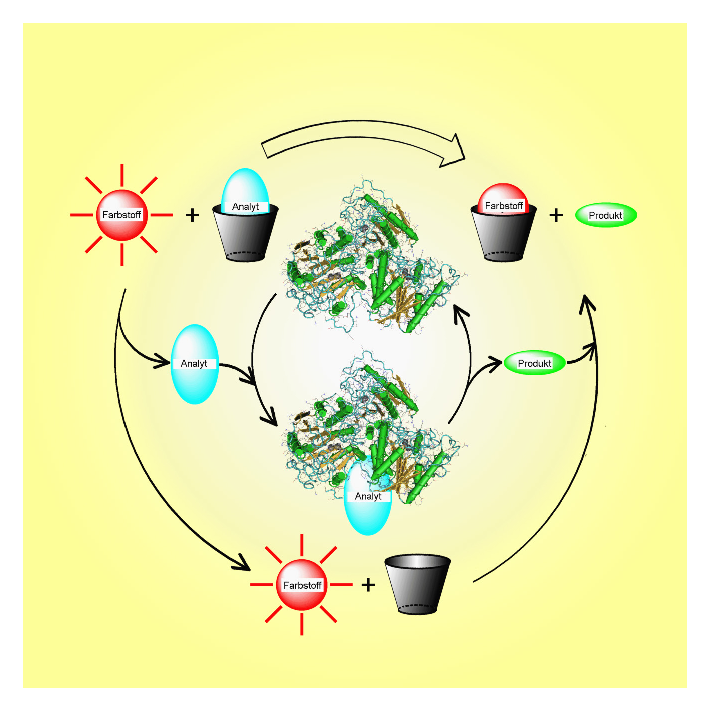
\includegraphics[width=\hsize]{Nau/Nau_2006_fig.pdf}
    \mycaption{ Working principle of an IN-OFF tandem assay.}\label{fig:nau-bild}
   \end{center}
\end{figure}

The method requires that (1)
the substrate and product of the reaction have a different
affinity to the macrocyclic host and (2) that the fluorescent
properties of the fluorescent dye differ in its complexed (by the
macrocycle) and uncomplexed forms. The former is expected whenever
the hydrophobic or electrostatic properties of substrate and
product differ significantly. For the latter effect (variations in
fluorescence properties of dyes upon complexation) numerous
examples are already available in the literature. The working
principle illustrated in Figure \ref{fig:nau-bild} is such that the substrate and
product displace the fluorescent dye to different degrees from the
macrocyclic host, and this differential displacement can be
translated into a change of its fluorescence. The latter can be
monitored with high sensitivity by established techniques. In our
laboratory, we perform steady-state fluorescence measurements on a
Varian Cary Eclipse spectrofluorometer and time-resolved
fluorescence measurements on a time-correlated single photon
counting set-up.\newline \newline Werner Nau is also involved in ``Supramolecular Functional Materials and Metalloenyzme Models''.


%Pictures are to be included via:



\myparagraph{Collaborations}
%
Bremen Area Collaborations:
\begin{enumerate}
\item {\sl International University Bremen} \\ Prof. K. Brix \\ Dye Stabilization in Live Cells
\\ Prof. A. Jeltsch \\ Investigation of Peptide Dynamics
\\ Prof. U. Kortz and Dr. M. Dickman \\ Structural Investigations
in Host-Guest Chemistry
\\ Prof. R. Richards \\Hybrid Materials
based on Cucurbiturils and Silver and Gold Nanoparticles
\\ Dr. D.
Roccatano \\ Study of the dynamics in solution of small peptides
by Molecular Dynamics simulation and time-resolved spectroscopic
techniques
 \\ Prof. S. Springer \\ Fluorescence spectroscopy of recombinant MHC class I molecules
 \\ Prof. M. Zacharias \\ Dynamics of end-to-end Contact Formation of Small Peptides
\end{enumerate}
National \& International Collaborations:
\begin{enumerate}
\item {\sl Hoffmann-La Roche Pharmaceuticals, Basel, Switzerland} \\ Dr. T. Enderle, Dr. D. Roth \\ Kinase Assays
\item {\sl Georgetown University, Washington DC, USA} \\ Prof. R. Weiss \\ Diffusion and Antioxidants in Polymer Films
\item {\sl Babha Atomic research Center, Mumbai, India} \\ Dr. J. Mohanty, Dr. Bhasikuttan, Dr. H. Pal \\ Supramolecular Photochemistry
\item {\sl Universidad Politecnica de Valencia} \\ Dr. U. Pischel \\ Supramolecular Sensors and Free Radical Reactions
\item {\sl Schlosspark-Klinik, Berlin} \\ Dr. Carl Erb \\ Messung von Antioxidantien im Kammerwasser und Blutplasma
\item {\sl Yarmouk University} \\ Prof. N. Saleh \\ Supramolecular Stabilization of Fungizides
\end{enumerate}


\paragraph{Grants}
\begin{enumerate}
\item Funded by private industry, Hoffmann-La
Roche/Pharmaceuticals, \emph{Novel Fast Time-resolved Assays
Allowing Rational Design of Fluorescent Substrates for Proteases
and Tyrosine, Serine, and Threonine Kinases}, (March 2004 -
February 2007) \item Funded by DAAD,  Grant with the Ac��es
Integradas Luso-Alemas/DAAD- GRICES Program
\emph{Cucurbituril-Based Lanthanide- Antenna Conjugates as Novel
Luminescent Supramolecular Devices}, (January 2005 - December
2008)
\end{enumerate}

\paragraph{Other Support Grants}
\begin{enumerate}


\item  {Egyptian governmental Ph.D. fellowship (4 years) for Hamdy El Sheshtawy (Egypt, since
November 2006) }

\item {DAAD Research fellowship for Prof. Na'il
Saleh (Jordan, summer 2006)}

\item  {DFG Travel Grant to attend the
First Joint International Symposium on Macrocyclic and
Supramolecular Chemistry, June 2006, Victoria, Canada}

\end{enumerate}
\paragraph{Honors and Awards}
%
\begin{enumerate}
\item Executive Member of the Photochemistry Section of the Gesellschaft Deutscher Chemiker GDCh
\item Elsevier Ph.D. Photoscientist Bursary 2006 (Ph.D. thesis of Dr. Huseyin Bakirci)
\end{enumerate}

\paragraph{Patents}
\begin{enumerate}
\item W. M. Nau, H. Bakirci, A. Hennig, ``Determination of
Concentration Changes'', German patent registration 10 2006 023083.3.
\end{enumerate}

\nocite{Nau1,Nau2,Nau3,Nau4,Nau5,Nau6,Nau7,Nau8,Nau9,Nau10,Nau11,Nau12,Nau13,Nau14,Nau15,Nau16}

\putbib[combined]
\end{bibunit}

\begin{bibunit}[hplain]
\subsubsection{Protein Engineering}
\index{Schwaneberg, Ulrich}

\paragraph{Research Team}
%
Ulrich Schwaneberg (Professor), Alexander Schenk (Postdoc), Radivoje Prodanovic (Postdoc), Li-qing Zhao (Postdoc), Jovana Grujic (PhD Student), Josefa Caballero Hern�ndez (PhD Student), Carmen Momeu (PhD Student), Tuck Seng Wong (PhD Student), Kang Lan Tee (PhD Student), Ozana Onaca (PhD Student), Saskia Ihle (PhD Student), Milan Blanusa (PhD Student), Daniela Josuttis (BTA), Marina Linow (Head of Biotechnikum), Dr. Birgit Orthen (Associated, Head of BioHanse Bremen)\\


We are experts in biocatalyst engineering with a focus on directed
protein evolution. The core competence comprises the development
of novel methods for generating diversity on the gene level
(SeSaM: \cite{Schwaneberg8} \& \cite{Schwaneberg9} and novel high-throughput screening systems (\cite{Schwaneberg3}, \cite{Schwaneberg5} \&
\cite{Schwaneberg7}). SeSaM method is complemented by a statistical method named MAP
(Mutagenesis Assistant Program) to provide protein engineers for
the first time with a tool to benchmark current random mutagenesis
methods by investigating the consequences of mutational bias on
the protein level. Based on these core competences we collaborate
with companies (e.g. BASF AG, BRAIN AG, Henkel KGaA, Schering AG,
Degussa AG) and research groups (mainly in Bremen, Hamburg, Basel
and Austin (USA)). In these collaborations we apply our developed
technologies to solve significant problems in industrial
biocatalysis and to understand structure-function relationships of
biocatalysts.



\paragraph{Highlights}
%
2006 was the year in which we published our first articles in the
Miniature Biofuel Cell and Nanocompartment area. These now
established research fields open novel and innovative directions
for our future research activities (see Figure). Highlights in
2006 comprise: a) publication of 12 manuscripts in peer-reviewed
journals including one cover page in JMB; four manuscripts have
been published with colleagues at Jacobs University (Dr. Roccatano, Prof.
Zacharias, Prof. Winterhalter), b) successful establishment of the
SeSaM Profit Center for commercial exploitation of the
SeSaM-mutagenesis technology. A lighthouse project for the company
BRAIN AG was successfully completed in 2006, an evolved
biocatalyst is in the upscale process at BASF AG, and the
SeSaM-Biotech company will become operational in October 2007, c)
additional secrecy agreements have been signed with Henkel KGaA,
Degussa AG and BRAIN AG to exploit the SeSaM-Technology, d) a 430
T Euro award from the BMBF has been granted for pushing screening
technologies, e) a DFG workshop for the SPP1170 ``Gelenkte
Evolution'' has been organized on Jacobs University campus, and f) a BioHanse
Bremen competence center for coordinating academic biotechnology
activities in Bremen  was established with the ``Gesch�ftsstelle''
at Jacobs University (200 T Euro award; State of Bremen).

\begin{figure}[ht]
  \begin{center}
    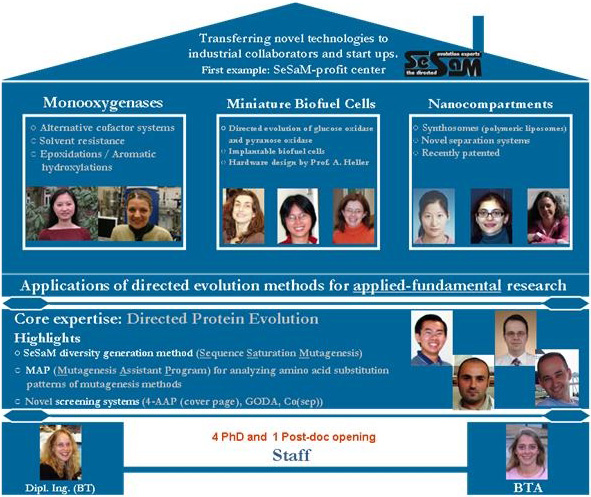
\includegraphics[width=\hsize]{Schwaneberg/Schwaneberg_2006_fig.png}
     \mycaption{Schwaneberg Research Group.}
  \end{center}
\end{figure}


\paragraph{Grants}
\begin{enumerate}
\item   Funded by ESF-COST, \emph{COST-D25-Biooxidation},
(November 2003   - October 2006)
 \item   Funded by BASF,  \emph{Esterase" und "Protease}, (April
2005  - March 2006)
 \item   Funded by DFG,
\emph{SeSaM, Sequence Saturation Mutagenesis and its application
in bioelectrocatalysis}, (September 2004  - August 2006)
 \item Funded by DBU, \emph{ICBio, Hochselektive
Bioaktivierung von Plattform-Intermediaten: Molekulares Screening,
funktionale �berexpression und umweltfreundliche elektrochemische
Verfahren}, (July 2004   -   June 2006)
 \item   Funded by SfBW - SfBUV, \emph{Selektive Isolierung von DNA und RNA in
Nanokontainern},  (January 2005    -   December 2007)
 \item
Funded by SfBW,  \emph{Bio-Hanse Bremen - Einrichtung eines
Kompetenzzentrums f�r Biotechnologie  }, (November 2005 - October
2007)
 \item Funded by DFG. \emph{Schw-2 Iterative
cycles, Understanding mediated/direct electron transfer and
solvent resistance by iterative cycles of directed monooxygenase
evolution and refinement of computational models },
(September 2006  -   August 2008)
 \item   Funded by BMBF,  \emph{BioChancePlus-BRAIN, Universelle
Hochdurchsatzdurchmusterungssystemen zum Auffinden industriell
bedeutsamer Biokatalysatoren in Metagenom-und
Zufallsmutagenese-Bibliotheken }, ( October 2006 - September 2009)

\item Funded by ONR, \emph{Making Glucose Oxidizing Enzymes Fit
for Biofuel Cell Applications}, (October 2002 - May 2006)
\end{enumerate}


\paragraph{Organization}
\begin{enumerate}
\item {Member of the Directorate and cofounder of the competence
center BioHanse Bremen and Bremen School of Biotechnology}
\item {Establishment of the SeSaM-profit center for exploiting the
economic potential of the SeSaM technology}
\end{enumerate}


\paragraph{Patents}

Two patents based on research at IUB. Eight patents in total (five
in collaboration with BASF AG)


\paragraph{Collaborations}
We are open to use our core competence in directed protein
evolution to study interesting structure-function relationships in
collaborative research effort with colleagues. An example is the
collaboration with the computational group of Prof. Zacharias/Dr.
Roccatano (four joint manuscripts), who provides and develops for
our evolved monooxygenase mutants (improved organic solvent
resistance, changes substrate specificity) rational design tools
and assists in statistical analysis of random mutagenesis mutants.
A further example is the nanocompartment system, which comprises
the collaborative work with two polymer chemists (Prof. Meier, who
moved from Jacobs University to Uni Basel; Stephan F\"{o}rster, Uni Hamburg) and
with Prof. Winterhalter (Professor for Biophysics), who probes the
compound flux through the channel proteins (1 joint publication).
We further collaborate with Prof. Wilmanns (DESY, EMBL, Hamburg;
one joint manuscript submitted) and various colleagues at Uni
Bremen (e.g. Prof. Jastorff, one manuscript in preparation),
Hochschule Bremen and Hochschule Bremerhaven. We have further
established collaborative projects or submitted joint grant
applications with Prof. Sun (Wuxi, China), Prof. Ma Yanhe
(Beijing, China), Prof. Socaciou (Rumania), Prof. Janssen
(The Netherlands), and Prof. Jankov (Serbia).


%\myparagraph{Collaborations}
%
%Bremen Area Collaborations:
%\begin{enumerate}
%\item {\sl Jacobs University Bremen} \\ Prof. F.O. Gl�ckner \\ Sulfatases
%\item {\sl Jacobs University Bremen}\\Prof. M. Zacharias and Dr. D. Roccatano \\Influence of Organic Cosolvents on the Industrially Important Enzyme P450 BM-3
%\end{enumerate}
%National \& International Collaborations:
%\begin{enumerate}
%\item{}
%\end{enumerate}

\nocite{Schwaneberg1,Schwaneberg2,Schwaneberg3,Schwaneberg4,Schwaneberg5,Schwaneberg6,Schwaneberg7,Schwaneberg8,Schwaneberg9,Schwaneberg10,Schwaneberg11,Schwaneberg12}

\putbib[combined]
\end{bibunit}

\begin{bibunit}[hplain]
\subsubsection{Downstream Processing}
\index{Fernandez-Lahore, Marcelo}


\paragraph{Research Team}
%
Marcelo Fernandez-Lahore (Professor), Sabine Binner (Technical Assistant), Rosa Cabrera (Postdoc), Rami Reddy Vennapusa (PhD Student), Farnoosh Dairpoosh (PhD Student), Leonardo Galvis (Graduate Student), Rustem Khusainov (Graduate Student)\\


Our work at Jacobs University has the main goal of the meta-integration between
the various bioproduct purification strategies that have been described
 previously in an isolate manner. The prefix meta- is thus
 ``used with the name of a discipline to designate a new but
  related discipline designed to deal critically with the original one''
  (Webster Dictionary). Up to now, no general rules exist on how to
   combine in the more efficient way process technology, combinatorial
   techniques, and genetic engineering tools. We are exploring this situation
    utilising a number of relevant industrial (bio) products. From the knowledge generated within the frame of our project(s) it is expected that general recommendations to guide industrialists will emerge. Clearly, this will translate in facilitated bioprocessing.

\paragraph{Highlights}
%
We have developed a novel Definitive Bioseparation Engineering concept based on mass screening experiments to exactly define de nature of the ``purification proteome'' for the chosen product expression system. ``Proteome spaces'' where proteins from the expression system are minimized or inexistent are being identified. Directing the targeted product to the same will allow attaining $-$or at least to very closely approaching$-$ the ``one-binding species'' situation. We have already shown that under these conditions prediction of large-scale processes is possible on the basis of simple analytical equations. Changing the relative ``proteome coordinates'' between product and contaminants will be attempted by introduction of protein tags or via dedicated ligand chemistry. Evidence-based results from scouting experiments will be compared to the expected binding of MS/MS identified host proteins to immobilized functional adsorbent groups. Emphasis will be on understanding the influence of the
 chemical environment provided by the solid phase, coupling chemistry and nature of the ligand in relation with protein surface.


\begin{figure}[ht]
  \begin{center}
   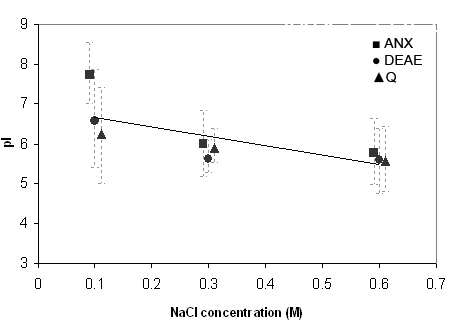
\includegraphics[width=\hsize]{Fernandez-Lahore/Fernandez-Lahore_new.png}
    \mycaption{Mean \& SD of isoelectric point values among the observed spots and the relationship between these values and the NaCl concentration of the corresponding material.}\label{fig2:Lahore}
     \end{center}
\end{figure}

%Achtung
Cell disruption constitutes and essential processing step for yeast
intracellular products, which is known to influence the quality of
fluidization and the sorption performance in `expanded' bed systems.
Cell electro-permeabilization coupled to direct product sorption on
expanded beds contactors was explored. S. cerevisiae F17 was pulsated in
batch mode (10 pulses, 1.5 ms, 4kV/cm, 2 Hz) and the properties of the
resulting cell particles studied via surface thermodynamic approaches.
Several process-relevant observations were made: a) The enzyme utilized
as model glyceraldehyde-3-phosphate dehydrogenase, GAPDH- was
released with high yield (87\%) and good purification factor (1.5-2.0)
in comparison with cell lysate as control; b) A shift in the surface
properties of the cell particles was noticed e.g., the Z-potential
changed from -12 mV to -9 mV upon pulsation while AB (-55 mN/m) and LW
(+30 mN/m) components suffered only minor change
at pH 7; c) A reduced interaction of the electroextracted feedstock with
DEAE-Streamline adsorbents was evidenced by the biomass pulse method
i.e. cell transmission increased from 14\% to 41\% after pulsation; and
d) the model product was purified by direct contact with a global yield
of 59-76\% and purification factor of 12. Moreover, low protease
activity was also observed i.e., 20\% of the activity present in the
mechanically disrupted cell paste.
A novel primary recovery route for yeast intracellular bioproducts can
be proposed by combination of selective permeabilization and immediate
sequestration on a solid phase. This will translate in increased product
quality, process yield, and cost-effectiveness.


%Cell disruption constitutes and essential processing step for yeast intracellular products, which is known to influence the quality of fluidization and the sorption performance in `expanded' bed systems.
%Cell electro-permeabilization coupled to direct product sorption on expanded beds contactors was explored. S. cerevisiae F17 was pulsated in batch mode (10 pulses, 1.5 ms, 4kV/cm, 2 Hz) and the properties of the resulting cell particles studied via surface thermodynamic approaches.
%Several process-relevant observations were made: a) The enzyme utilized as model $-$glyceraldehyde-3-phosphate dehydrogenase, GAPDH- was released with high yield (87\%) and good purification factor (1.5-2.0) in comparison with cell lysate as control; b) A shift in the surface properties of the cell particles was noticed e.g., the Z-potential changed from $-$12 mV to $-$9 mV upon pulsation while AB (?+ 3-4 mN/m, ?- 51-55 mN/m) and LW (28-30 mN/m) components suffered only minor change at pH 7; c) A reduced interaction of the electroextracted feedstock with DEAE-Streamline adsorbents was evidenced by the biomass pulse method i.e. cell transmission increased from 14\% to 41\% after pulsation; and d) the model product was purified by direct contact with a global yield of 59-76\% and purification factor of ?12. Moreover, low protease activity was also observed i.e., ? 20\% of the activity present in the mechanically disrupted cell paste.
%A novel primary recovery route for yeast intracellular bioproducts can be proposed by combination of selective permeabilization and immediate sequestration on a solid phase. This will translate in increased product quality, process yield, and cost-effectiveness.


\myparagraph{Collaborations}
National \& International Collaborations:
\begin{enumerate}
\item {\sl National University of Quilmes (Buenos Aires)} \\ Prof.  M. Grasselli \\ Novel materials for downstream processing of bioproducts
\item {\sl Pablo Cassara Foundation (Buenos Aires)}  Dr. M.A. Alvarez \\ Molecular Pharming
\end{enumerate}


\nocite{Fernandez-Lahore1,Fernandez-Lahore2,Fernandez-Lahore3,Fernandez-Lahore4,Fernandez-Lahore5,Fernandez-Lahore6,Fernandez-Lahore7}
\putbib[combined]
\end{bibunit}

\begin{bibunit}[hplain]
\subsubsection{Computational Bioengineering}
\index{Roccatano, Danilo}

\paragraph{Research Team}
Danilo Roccatano (University Lecturer (Chemistry))\\

The investigation of physico-chemical properties of
biological  systems of industrial relevance using computational methods
is one of the major aspects of  my research. I am interested in
applying theoretical model and using molecular modelling to provide useful information
that drives enzyme evolution and protein engineering for biotechnological applications. Various aspects of my research activities are summarized below:\\

Study of the effects of non-aqueous solvents and their water mixtures on the
conformation, diffusive dynamics and reactivity of macromolecular systems for
bioengineering. In particular, the solvent effect on
protein folding and enzymatic activity is of high commercial and academic interest.\\

In collaboration with Prof. U. Schwaneberg and collaborators, we are committed to
developing computational tools to assist directed evolution experiments.~\cite{Wong06M,Schenk06M,Wong06bM}
As a long term project, we are developing a Computational Bioengineering Portal (map.iu-bremen.de)
comprising various programs that assist random mutagenesis experiments. This publicly available server is dedicated to directed evolution community.



\paragraph{Highlights}
Main research achievements in year 2006 are summarized as follow:\\


The  collaboration with Prof. U. Schwaneberg and his PhD student T.
S. Wong resulted in  important achievements:  MD simulations study
provided a clue on the mechanism of DMSO inactivation of heme
monooxygenase P450 BM-3~\cite{Roccatano06aM}.  A subsequent
resolution of the crystal structure of P450 BM-3 heme domain in
presence of DMSO, performed by T. S. Wong in collaboration with
Prof. M. Wilmanns at EMBL Hamburg, confirmed the theoretical
hypothesis and showed the
coordination of DMSO to the active site heme iron. \\

Setting up a Computational Bioengineering Portal at Jacobs University (map.iu-bremen.de) (Fig. \ref{fig:Roccatano2}).
The portal is dedicated to providing various computational
support for directed evolution. It includes Mutagenesis Assistant Program (MAP)~\cite{Wong06M,Schenk06M}
(running since beginning 2006, Fig. \ref{fig:Roccatano2}) that allows analyzing amino acid substitution patterns of 19 random mutagenesis methods upon input of a DNA sequence. Other two programs will be
available on the portal by the end of 2006, SeSaM-Tv and ExPoSeS. SeSaM-Tv is computational tool
to support Sequence Saturation Mutagenesis (SeSaM), a novel random mutagenesis method developed by T. S. Wong and Prof. U. Schwaneberg. ExPoSeS (Exploring Protein Sequence Space) provides guidance to efficiently explore protein sequence space using combinations of random mutagenesis methods.


\begin{figure}[ht]
  \begin{center}
   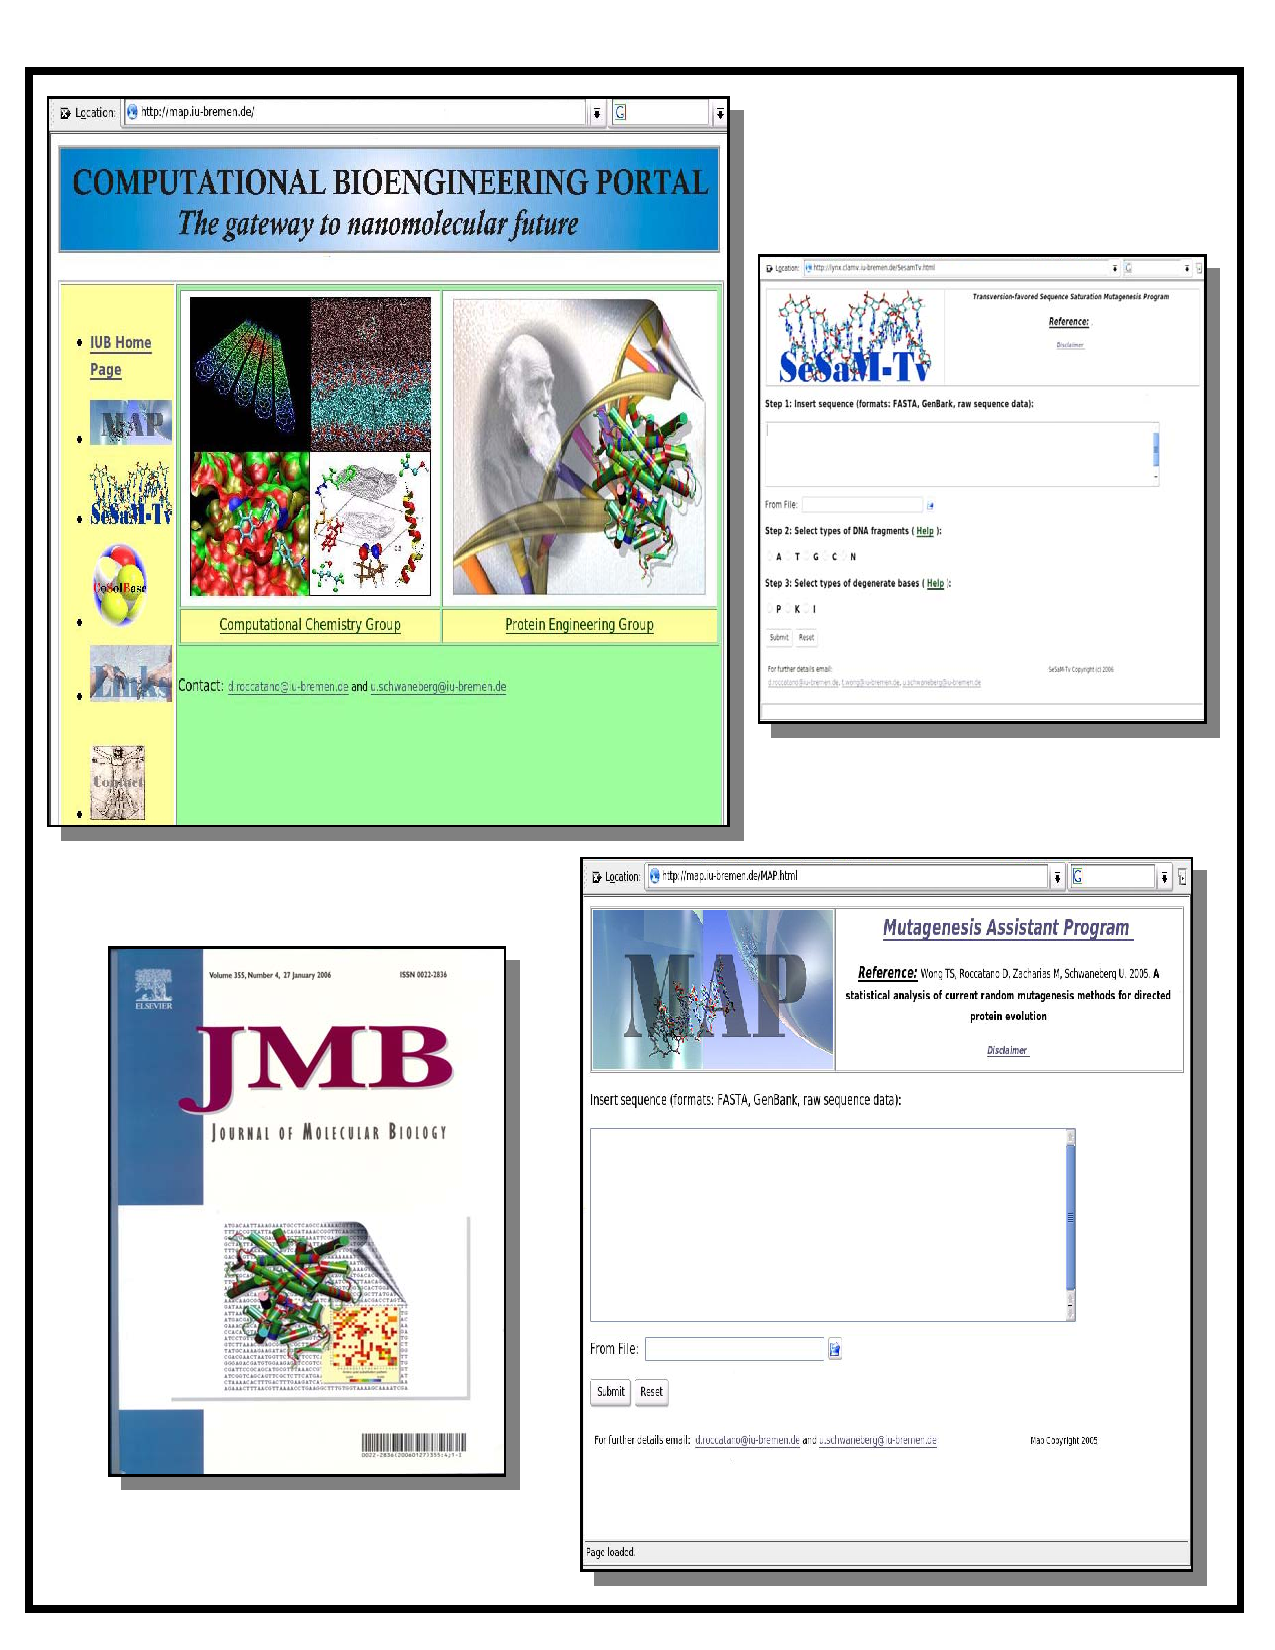
\includegraphics[width=\hsize]{Roccatano/DrRoccatano-fig2.pdf}
     \mycaption{The Computational Bioengineering Portal at Jacobs University (map.iu-
bremen.de).}\label{fig:Roccatano2}
   \end{center}
\end{figure}



Danilo Roccatano is also involved in ``Nano and Material Science''.


\myparagraph{Collaborations}
%
Bremen Area Collaborations:
\begin{enumerate}
\item {\sl International University Bremen} \\ Prof. W. Nau \\ Study of the dynamics in solution of small peptides by Molecular Dynamics simulation and time-resolved spectroscopic tecniques.
 \\ Prof. U. Schwaneberg \\ Study of  the organic solvent effects on monooxygenase P450 BM-3 and Mutagenesis Assistant Program.
 \\ Prof. M. Zacharias \\ Molecular Dynamics simulation study of the nucleosome core particle.
\end{enumerate}
National \& International Collaborations:
\begin{enumerate}
\item {\sl University of Salerno, Italy} \\ Prof. G. Milano \\ Interaction of polymer with biological membranes
\item {\sl University of East Anglia, Norwich, UK} \\ Dr. S. Hayward  \\ Theoretical investigation of domain motion in proteins
\item {\sl Max Planck Institute for Biophysical Chemistry, G�ttingen } \\Dr. B. de Groot \\ Theoretical investigation of domain motion in proteins
\end{enumerate}


\nocite{Pal06M,Roccatano06bM,Sahoo06M}

\putbib[combined]
\end{bibunit}


\shorttitle{Molecular Life Sciences}
\subsection{Molecular Life Sciences}
\label{MolLifeSc}

The Molecular Life Scientists at International University Bremen devote their research activities to the understanding of macromolecules and of the biochemical pathways which build up the units of life - our cells. The integration of cellular functions in the broader context of natural biological systems is an important aim of the research groups involved. A strong focus is set out to uncover the molecular mechanisms which maintain vital functions of healthy life. Hence, main expertise and research activities of Molecular Life Scientists are in the field of Molecular Medicine. The aim is to identify targets for drug design for the development of better treatments and therapies of diseases which challenge the modern world.\\

Our motivation is to combine basic sciences, modeling and simulation approaches, biochemical, cell and molecular biological approaches, assays employing organismic model systems as well as analyses of environmental habitats in order to answer key questions concerning the organisms of all divisions of life. \\

Key-questions of the research groups of the Molecular Life Sciences
at IUB comprise the understanding of
\begin{myitemize}
\item   DNA methylation as an important regulator for gene expression in bacteria and mammals,
\item   the concerted rearrangements of gene expression during growth and development,
\item   the significance of protein degradation for proper function of epithelial organs in adult mammalian organisms,
\item   the importance of brain glial cells for development of neurodegenerative diseases,
\item   the molecular mechanisms of the anti-viral immune response,
\item   the importance of virulence factors of plants during their response against  phytopathogens,
\item   molecular interactions of marine bacteria with each other and with phytoplankton cells,
\item   characteristics of diverse microbial habitats in the ocean, and
\item   the interaction of chemicals with marine life for the identification of biomarkers to predict toxic effects.\\
\end{myitemize}


Centrally important are the interactions between the groups that allow us to study molecular mechanisms and to deduce principles which are of significance for the complexity of all biological systems. Underlying principles governing gene expression and hence, proliferation and differentiation of cells are covered to a comparable extent as principles regulating the interaction of microbes, plants, and animals that live in terrestric and marine habitats.\\


\begin{bibunit}[hplain]
\subsubsection{Biochemistry - Methyltransferases}
\index{Jeltsch, Albert}

\paragraph{Research Team}
%
Albert Jeltsch (Professor),
Sandra Becker (Technician),
Sanjay Chahar (PhD Student),
Arunkumar Dhayalan (PhD Student),
Renata Jurkowska (PhD Student),
Tomek Jurkowski (PhD Student),
Heike Laser (Postdoc),
Kirsten Liebert (Postdoc),
Sergei Ragozin (Postdoc),
Philipp Rathert (PhD Student),
Christian Rohde (PhD Student),
Martina Schlickenrieder (PhD Student),
Maike Schwerdtfeger (Lab Technician),
Yinying Zhang (PhD Student)\\

DNA methylation is an important regulator for gene expression in mammals. Methylation of human DNA at CG sites is a central trigger for cellular differentiation and gene regulation. In bacteria, DNA methylation is involved in various processes including DNA repair, gene regulation, phase variation and pathogenicity. We study the DNA recognition, structure and enzymatic mechanism of prokaryotic DNA methyltransferases from E.coli, phages, Salmonella and other bacteria with the aim to develop specific inhibitors for these enzymes that are potentially active as antibiotics. Mammalian enzymes are studied to understand the process of generation and preservation of methylation patterns in human cells. We are involved in approaches to analyze the methylation pattern of human DNA. The results will allow understanding differentiation and gene regulation at better level which is a pre- requisite for successful application of cloning procedures for organ replacement in the future.


\paragraph{Highlights}

The specific interaction of proteins with DNA is a fundamental process in the regulation of gene expression in all organisms. In collaboration with the group of  X. Cheng (Atlanta, GR) we have solved the structure of the EcoDam DNA methyltransferase and elucidated how this enzyme specifically recognizes its GATC target site on DNA. The structural analysis revealed that the enzyme forms four specific interactions to the bases of the DNA, the importance of these contacts was confirmed by biochemical studies with enzyme variants after removal of some of the important residues. One striking result of that study was that the process of contacting the DNA resembles closing of a zipper in which the interactions on one site of the target are formed earlier while others follow in an ordered pathway. Changing of the amino acid residues that contact the DNA allowed to modify the DNA interaction of the enzyme and create enzyme variant with new DNA recognition specificities. These results shed light on the principles of protein/DNA interactions. Furthermore, the detailed structural and functional knowledge about the dam DNA methyltransferase might enable us in the future to design new types of antibiotics which inactivate this protein, which has been shown to be important for pathogenicity in several important human pathogens.

\begin{figure}[ht]
  \begin{center}
   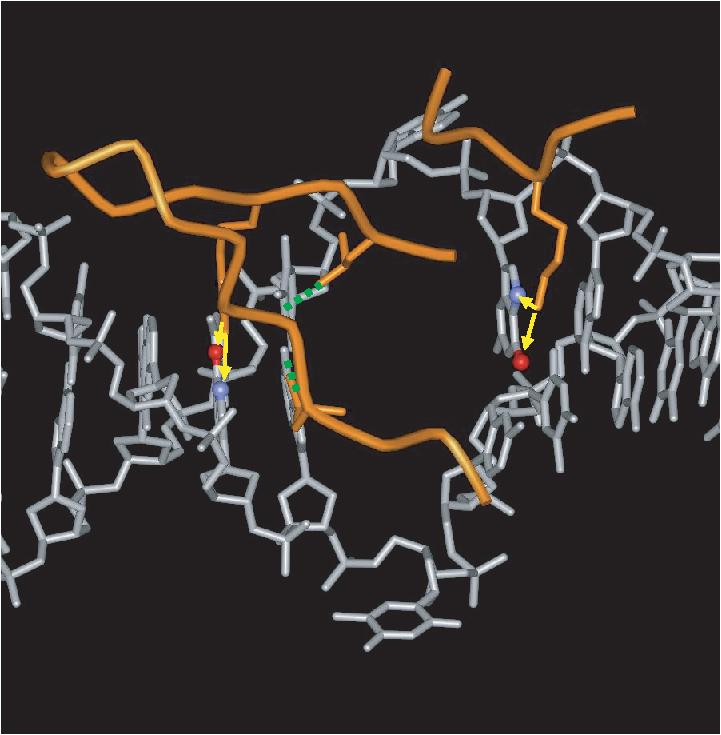
\includegraphics[width=\hsize]{Jeltsch/Fig_Jeltsch1_2006.pdf}
    \mycaption{Structure of the Ecodam Methyltransferase in complex with specific DNA.}\label{Fig_Jeltsch1_2006.pdf}
   \end{center}
\end{figure}

In a second project, we study the function of mammalian DNA methyltransferases. In mammals, the DNA methylation pattern is copied during each round of DNA replication. In cooperation with R. Reinhardt (Berlin, Germany) we have studied the mechanism and specificity of the Dnmt1 enzyme which has a central role in copying the pattern of DNA methylation after replication and thereby mediates epigenetic inheritance of the patterns of gene expression in various cell types. Using long hemimethylated DNA substrates that carry defined methylation patterns and bisulfite analysis of the methylation reaction products, we show that the enzyme has a 15 fold preference for hemimethylated CG sites. Dnmt1 moves along the DNA in a random walk methylating hemimethylated substrates with high processivity ($>$50 sites are visited on average which corresponds to linear diffusion over 6000 base pairs). These properties are jmportant for the physiological function of Dnmt1.\newline \newline Albert Jeltsch is also involved in ``Enzyme Design''.

\myparagraph{Collaborations}
%
Bremen Area Collaborations:
\begin{enumerate}
%
\item {\sl International University Bremen} \\ Prof. K. Brix \\ Confocal cell imaging
 \\ Prof. G. Mushkelishvili \\ AFM of DNA methyltransferases
 \\ Prof. W. Nau \\ Investigation of Peptide Dynamics
\\ Prof. S. Springer \\ Rapid Kinetics
\\ Dr. H. Stamerjohanns \\ Data analysis and web programming
 \\ Prof. M. Ullrich \\ Mass spectrometry
 \\ Dr. C. Voelcker-Rehage \\ Genkotyping participants of the JC aging study
 \\ Prof. M. Winterhalter \\ Dynamic light scattering
 \\ Prof. M. Zacharias \\ Simulation of enzyme dynamics

\end{enumerate}
National \& International Collaborations:
\begin{enumerate}
\item {\sl University of Texas, Department of Carcinogenesis, Smithville, Texas, USA} \\ Prof. M.T. Bedford \\ Peptide interaction of DNA methyltransferases
\item {\sl Emory University Atlanta, Department of Medicine, GA, USA} \\ Prof. X. Cheng \\ X-ray crystallography and inhibitor design of DNA methyltransferases
\item {\sl Universit�t Halle} \\ Prof. R. Dammann \\ Expression of Dnmt1 in cells
\item {\sl University of Edinburgh, Edinburgh, UK} \\ Prof. D.T.F. Dryden \\ Time resolved fluorescence spectroscopy with DNA methyltransferases
\item {\sl Laboratory of Cancer Epigenetics, Faculty of Medicine, Free University of Brussels, Brussels, Belgium} \\ Prof. F. Fuks \\Phosphorylation of DNA methyltransferases
\item {\sl DKFZ, Heidelberg} \\ Prof. I. Grummt \\ Regulation of DNA methyltransferases in cells
\item {\sl Hungarian Academy of Science, Szeged, HU} \\ Prof.  A. Kiss \\ Expression and Design of the M.SssI DNA methyltransferase
\item {\sl Department of Biochemistry and Molecular Biology, University of Shaanxi, China} \\ Dr. F. Li \\Targeted methylation of DNA in cells
\item {\sl DKFZ, Heidelberg} \\ Dr. F. Lyko \\ Expression and characterisation of Dnmt2
\item {\sl University of Groningen, Groningen, The Netherlands} \\ Dr. P. McLaughlin\\ Targeted methylation of DNA in cells
\item {\sl National Cancer Institute, Frederick, MD, USA} \\ Prof. K. Muegge \\ Regulation of Dnmt3a in cells
\item {\sl Institut f�r Genetik, Universit�t Kassel} \\Prof. W. Nellen \\ Expression and characterisation of Dnmt2
\item {\sl The Wellcome Trust Biocentre, University of Dundee, Dundee, UK} \\ Prof. T. Owen-Hughes \\ Preparation of nucleosomal DNA
\item {\sl MRC, Cambridge, UK} \\ Dr. M. Papworth\\ Targeted methylation of DNA in cells
\item {\sl Leibnitz Institute for Age Research, Jena} \\ Dr. M. Platzer \\ High troughput DNA Sequencing
\item {\sl Justus-Liebig Universit�t Giessen} \\ Prof. A. Pingoud \\ Targeted DNA cleavage
\item {\sl MPI f�r Molekulare  Genetik, Berlin }\\ Dr. R. Reinhardt \\ High troughput DNA sequencing
\item {\sl CNRS/University of Rennes 1 Joint Unit, Rennes, France} \\ Dr. G. Salbert \\ Enzymology of Dnmt3a
\item {\sl MHH, Hannover \\ Prof. C. Urbanke} \\ Analytical Ultracentrifugation
\item {\sl Universit�t Saarbr�cken} \\ Prof. J. Walter \\Human Methylome analysis
\item {\sl Chinese Academy of Sciences, Shanghai, China} \\ Prof. G. Xu \\ Biologcial role of Dnmt3a
\end{enumerate}

\paragraph{Organization}
%
\begin{enumerate}
\item {Member of the editorial board of BMC Biochemsitry}
\end{enumerate}

 \paragraph{Grants}
\begin{enumerate}
\item Funded by BMBF, Biofuture \emph{Development of programmable
DNA methyltransferases for biotechnological applications },
(August 2003 - Dezember 2007)
 \item
Funded by BMBF,  BioChancePlus \emph{Amplification of DNA with
preservation of the methylation state }, (May 2004 - April 2007)

\item Funded by BMBF,  SMP Epigenetics \emph{Analysis of the DNA
methylation pattern of genes on Chromosome 21 } , (May 2005 -
April 2007)

\item Funded by NIH (USA), \emph{Histone Lysine Methylation:
structures and functions},  (October 2006 - September 2011)

\item Funded by DFG,  priority program SPP1070 \emph{Directed
evolution of DNA methyltransferases}, JE252/5-1 and 5-2,
 (September 2004 - May 2007) (JE252/5-1), (December 2006 -
December 2008) (JE252/5-2)

\item Funded by DFG,  priority program SPP1129 \emph{Biochemistry
and biological function of mammalian Dnmt1 and Dnmt2}, JE252/4-2
and 4-3, (December 2005 - November 2007) (JE252/4-2), (October
2006 - December 2008) (JE252/4-3)

\item Funded by DFG, \emph{Enzymology, structure and DNA
recognition of the E. coli dam DNA methyltransferase}, JE252/2-6,
(October 2005 - December 2008)




\end{enumerate}

\paragraph{Other Support Grants}
\begin{enumerate}
\item {JE252/2-5 (DFG) ``Enzymology, structure and DNA recognition of the E. coli dam DNA methyltransferase'' at University of Gie\ss en}
\item {HBFG 066/7-1 (DFG) ``Purchase of a MALDI TOF mass spectrometer''}
\end{enumerate}


\paragraph{Patents}
\begin{enumerate}
\item {Patent application: Pingoud, Jeltsch, Eisenschmidt: Hochspezifisch mit DNA interagierende Enzym-Konjugate. EPA 2005/009028 (pending)}
\item {Cheng, Horton, Yang, Calman, Zhang, Jeltsch, Hattmann ``Small Molecule Inhibitors of Bacterial Dam DNA Methyltransferases'', PCT Patent Application No. PCT/US 05/44277, 2006 (pending)}
\end{enumerate}


\paragraph{Awards, Prices}
\begin{enumerate}
\item {Elected as vice-president of the DNA Methylation Society (New Orleans, LO)}
\end{enumerate}


\nocite{Jeltsch1,Jeltsch2,Jeltsch3,Jeltsch4,Jeltsch5,Jeltsch6,Jeltsch7,Jeltsch8,Jeltsch9,Jeltsch10}

\putbib[combined]
\end{bibunit}

\begin{bibunit}[hplain]
\subsubsection{Molecular Genetics - Gene Regulatory Networks}
\index{Muskhelishvili, Georgi}

\paragraph{Research Team}
%
Georgi Muskhelishvili (Professor), Claudia Burau (Lab Technician), Michael Berger (PhD Student),
Marcel Geertz (PhD Student), Sebastian Maurer (PhD Student), Ramesh Mavathur (PhD Student)\\


The understanding of concerted rearrangements of gene expression during growth and development is a fundamental problem. Since gene regulation is most pervasive at the transcriptional level, the essential question is how the transcription machinery is directed to different types of gene promoter in a spatially and temporally ordered way. We are investigating this problem in the classical model organism \textit{Escherichia coli}. In this organism the gene promoter recognition depends on the binding specificity of distinct RNA polymerase initiation sigma subunits, which can be modulated by interactions with small effector molecules and protein cofactors. In addition, the accessibility of cellular gene promoters depends on the chromatin architecture. This latter is determined by binding of abundant DNA architectural proteins and the supercoiling level of chromosomal DNA, whereby the supercoiling level reflects the metabolic state of the cell. Our goal is the development of a general model of coordinated gene transcription implicating a unique interdependence between DNA topology, chromatin architecture, transcription machinery composition and the metabolic state of the cell. Due to the complexity of the problem under study we employ a wide diversity of methods including approaches of transcriptomics, proteomics, fluorescent microscopy, atomic force microscopy, bioinformatics and molecular modeling and also different methods of biochemistry, biophysics and molecular genetics for detailed analyses of unique genes.

\paragraph{Highlights}\noindent
%
The main scientific achievements in 2006 were:\\
 Publication of a research paper in \textit{EMBO reports} uncovering the homeostatic mechanism coordinating the growth phase-dependent gene transcription in bacterial cells (Fig. \ref{fig:Muskhelishvili-fig1}). This study reveals a tight coupling between chromosomal DNA supercoiling and the cellular metabolism thus providing a new logical space for understanding the organization of metabolic pathways. The performed experimental work is based on a DNA microarray-based approach developed in my group and providing a novel tool for context-dependent understanding of gene expression patterns. This approach identifies control mechanisms for large groups of essential genes and can be applied, in principle, to any living cell.


\begin{figure}[ht]
  \begin{center}
   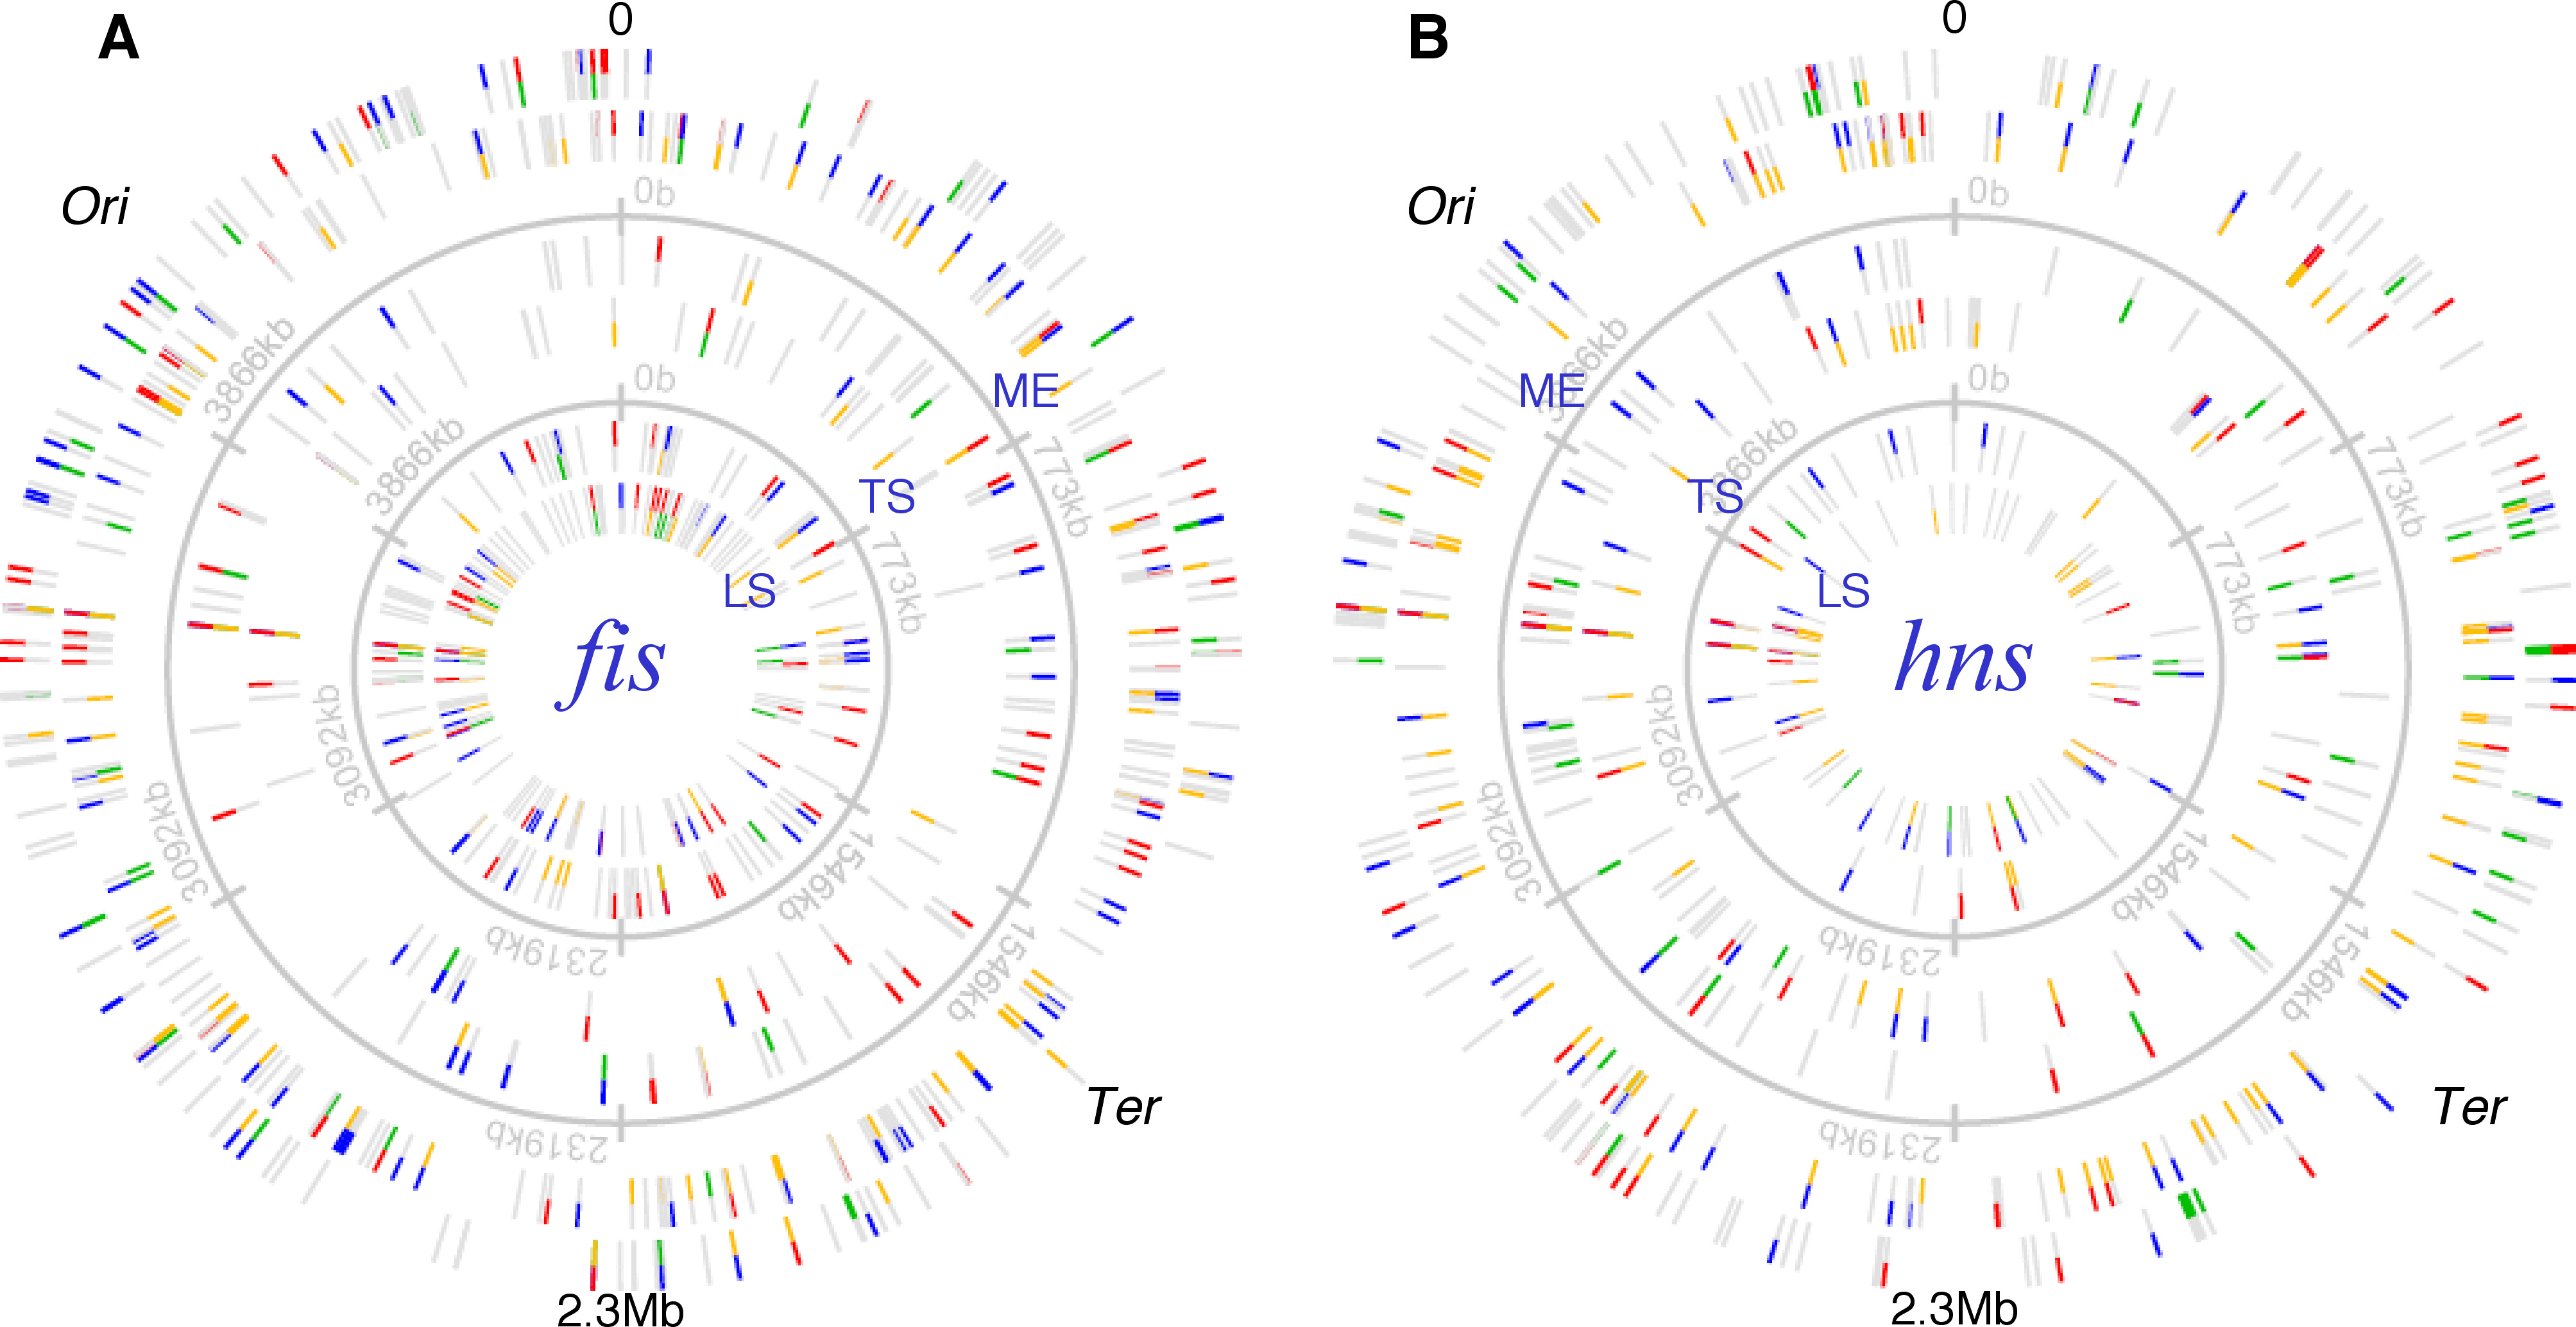
\includegraphics[width=\hsize]{Muskhelishvili/Muskhelishvili-fig1.png}
    \mycaption{\textit{Escherichia coli} genomic wheels showing the differential distributions of four classes of supercoiling-sensitive genes - \textit{Rel} (red), \textit{Hyp} (blue), \textit{Act} (green) and \textit{Rep} (yellow) - among the growth phase-dependent genes (grey) in CSH50 wild type (outer wheels) and mutant (inner wheels) strains. The mutants are lacking global gene regulators, either FIS or H-NS. \textbf{A.} CSH50 wild type vs \textit{fis} mutant. \textbf{B.} CSH50 wild type vs \textit{hns} mutant. \textit{Ori} and \textit{Ter} indicate the origin and terminus of chromosomal replication, respectively. ME, TS and LS indicate the mid-exponential, transition and late stationary growth phases, respectively.}\label{fig:Muskhelishvili-fig1}
   \end{center}
\end{figure}

Publication of a research paper in \textit{EMBO Journal} (together with J�rgen Fritz, Jacobs University, and Andrew Travers, MRC Cambridge) describing for the first time the structural organisation of a transcription initiation complex of major \textit{Escherichia coli} RNA polymerase holoenzyme and a transcriptional activator. The structure described in this article provides a new paradigm for the molecular mechanism of transcriptional regulation of gene expression in bacteria.

A theoretical paper proposing a unified model of molecular mechanisms of gene regulation in Eukaryotes and Prokaryotes has been written (together with my colleague Andrew Travers, MRC Cambridge) and accepted for publication in \textit{EMBO reports}.


A research paper together with Prof. Matthias Ullrich providing new insights into the transcriptional organization of the \textit{algT-muc} gene cluster of \textit{Pseudomonas syringae pv. Glycinea} published in \textit{Journal of Bacteriology}.

A research paper together with colleagues from MRC Cambridge, Ecole Normale Superieure de Cachan, and the University of Camerino describing the identification of the binding site consensus sequence for the global regulator H-NS is in the final stage of preparation. This article provides first clues to the understanding of the mechanistic role of H-NS regulatory protein in virulence gene expression during infectious diseases caused by enteropathogenic \textit{Escherichia coli} and \textit{Salmolla}.


\paragraph{Collaborations}

Bremen Area Collaborations:
\begin{enumerate}
\item {\sl International University Bremen} \\ Prof. K. Brix \\ Confocal microscopy
 \\ Prof. M. Fernandez-Lahore \\Proteomics
 \\ Prof. J. Fritz \\ Atomic force microscopy
 \\ Prof. F.O. Gl�ckner \\ Transcriptomics
 \\ Prof. M.-Th. H�tt \\ Gene regulation networks
\\ Prof. A. Jeltsch \\ Methylation and transcription
 \\ Prof. M. Ullrich \\ Promoter mapping
\\ Prof. M. Zacharias \\ Molecular modeling
\\ Hildegard Meyer-Ortmanns\\ Modeling networks
\end{enumerate}
National \& International Collaborations:
\begin{enumerate}
\item {\sl MRC Cambridge, UK} \\ Dr. A. Travers \\ DNA topology and gene expression
\item {\sl Ecole Normale Superieure de Cachan, France} \\ Dr. M. Buckle \\ DNA binding proteins
\item {\sl Universita di Camerino, Italy} \\ Prof. C. Gualerzi \\ DNA binding proteins
\item {\sl University of Lyon, INSA de Lyon, France} \\ Dr. W. Nasser \\ Regulation of bacterial virulence
\item {\sl National Instutute of Genetics, Mishima, Japan} \\ Prof. N. Shimamoto \\ Regulation of transcription
\end{enumerate}

\paragraph{Grants}
%
\begin{enumerate}
\item Funded by DFG,  \emph{Elucidation of the mechanism of
growth-dependent gene regulation by the \textit{Escherichia coli}
global transcription factor FIS},  grant MU 1549/2-2, (October
2005 - September 2008)
\end{enumerate}

\nocite{Muskhelishvili1,Muskhelishvili2,Muskhelishvili3,Muskhelishvili4,Muskhelishvili5}

\putbib[combined]
\end{bibunit}

\begin{bibunit}[hplain]
\subsubsection{Molecular Cell Biology - Biomedicine of Proteolysis}
\index{Brix, Klaudia}

\paragraph{Research Team}

Klaudia Brix (Professor), Heiko B�th (PhD completed in April 2006), Stefanie Dannenmann (Graduate Student), Anna Dunkhorst (PhD Student), Silvia Jordans (PhD completed in February 2006, Postdoctoral Fellow), Malgorzata Kubica (Visiting PhD Student), Kristina Mayer (PhD completed in January 2006, Postdoctoral Fellow), Hong Qu (PhD completed in May 2006), Maren Rehders / Meike Klepsch (Lab Technicians), Lakshmi Settu (Graduate Student), Ruxandra Sirbulescu (Graduate Student), Brit Wolters (PhD completed in March 2006)\\

Our research focus is to understand epithelial organs such as intestine, skin, and thyroid on the cellular and molecular level. As a biomedically-oriented group, our goal is to analyze the functions of these organs and to propose concepts, which might help in the development of novel therapeutic strategies. Our research is focused on proteolytic processes performed by lysosomal cysteine cathepsins. Using a combination of biochemical, cell and molecular biological research approaches, we analyze the spatio-temporal regulation of proteolysis and protease interaction in networks existing in defined biological systems of mammalian organisms. Thus, we get more insight into a general understanding of proteolytic processes in order to interfere with immobility of the gut with its most severe clinical complication of intestinal atony, scar formation as a result of improper wound healing of the skin, and dysfunction of the thyroid resulting in hormone deficits.

\paragraph{Highlights}
%
The main task of the thyroid gland is the production of thyroid hormones which are essential for brain development, growth, and regulation of metabolism and body temperature. Disorders of the thyroid are frequently observed. Hypothyroidism and goiter may arise as a result of iodine deficiency. In severe cases of low-iodine diets the phenotype of cretinism still occurs. We identified thyroglobulin, the precursor of thyroid hormones, as one of the natural  substrates of lysosomal cysteine peptidases. Through the use of cathepsin-deficient mouse models, we showed that the intra- and extracellular actions of cathepsins B, K, and L maintain thyroid function. Recently, we began to investigate the significance of cysteine cathepsin K for proper brain development in mouse models by combining behavioral studies with biochemical and cell biological approaches in order to explain the observed learning and memory phenotypes on the molecular level.

In cell-based assays, trafficking analyses were performed that comprised expression of GFP-tagged cathepsins with or without active-site-mutations, and cathepsin variants derived from tumor cells, as well as the use of activity-based probes to visualize transport and proteolytic activities of the enzymes in living cells. The results proved that the primary sequence and proper folding of the proteases is sufficient to correctly target cysteine cathepsins into endocytic compartments of normal epithelial cells. However, altered trafficking in carcinoma cells often results in mislocalization of cysteine cathepsins. Hence, cellular transport logistics do not depend on the cargo but rather on the cells themselves. This notion bears important implications for the molecular mechanisms underlying altered transport pathways of cysteine cathepsins in pathological conditions such as cancer.

During regeneration from wounding, secreted cathepsin B mediates keratinocyte migration for rapid wound closure by proteolysis and remodeling of the extracellular matrix. Specific receptors at the plasma membrane ensure restriction of the proteolytic activity of cathepsin B to the basal pole of the migratory cells. In contrast, trafficking of cathepsins L and V follows different routes in keratinocytes. Cathepsin L remains largely unaffected when human keratinocyte cell lines were wounded. However, a truncated version of cathepsin V is translocated to the nuclei of regenerating cells before keratinocytes start to proliferate. Future experiments aim to verify a causal relation between these two events and shall elucidate the molecular mechanisms that are initiated by the appearance of cathepsin V within the nuclei of keratinocytes.


\begin{figure}[ht]
  \begin{center}
   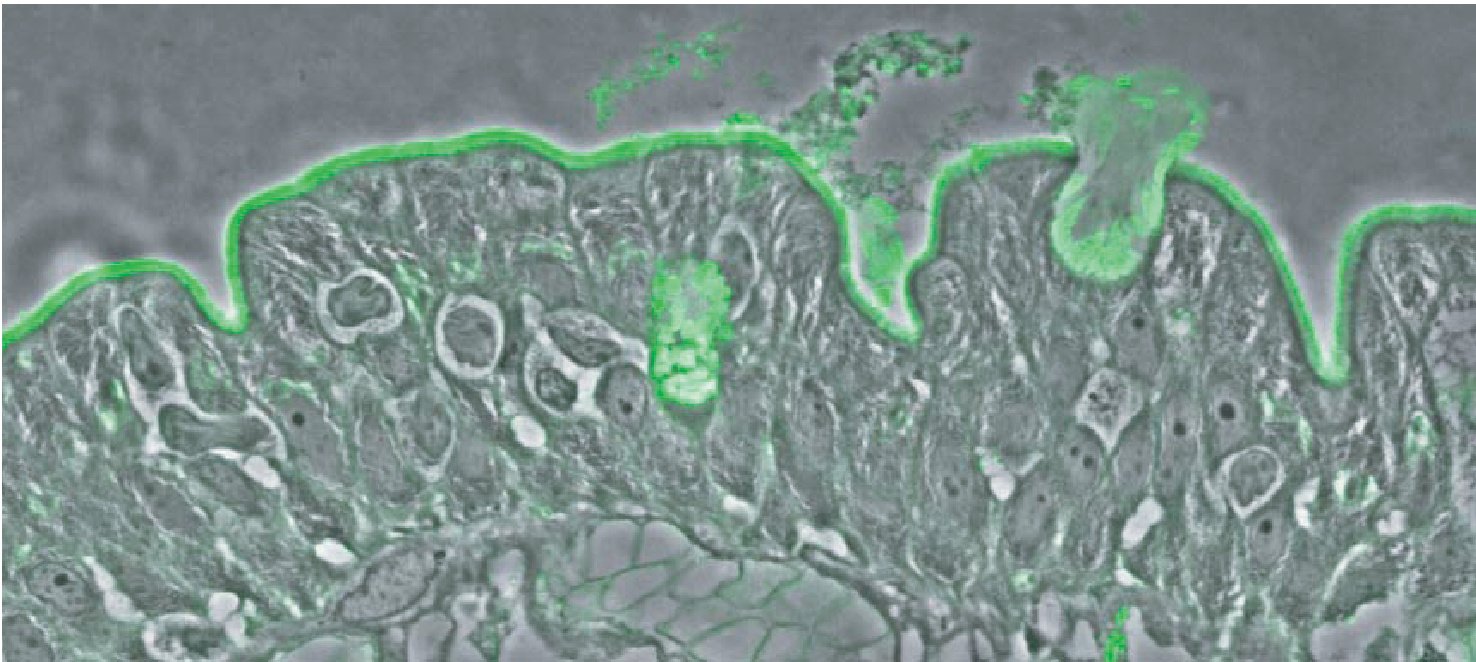
\includegraphics[width=\hsize]{Brix/Brix_2006_Fig.pdf}
    \mycaption{Cathepsin L expression in enterocytes and goblet cells of the mucosa of the small intestine; confocal laser scanning microsopy.}\label{fig:profBrix}
   \end{center}
\end{figure}


Recently, we hypothesized that non-regulated release of proteolytic enzymes as a result of tissue damage due to surgical trauma may have dramatic consequences for the affected tissue. Our studies on intestine trauma focus on the possible contribution of cathepsins to the onset of inflammatory responses, ultimately leading to dysfunction of intestinal smooth muscles and post-operative ileus, which is a severe and potentially life-threatening complication common in the clinics. Using standardized models of intestine trauma in mice and rats, we observed a local cathepsin B release concomitant with extracellular matrix damage during initial post-operative phases. Interestingly, cathepsin B-deficient animals showed an increased deposition of extracellular matrix components in the intestine. We concluded that the observed massive degradation of extracellular matrix in traumatized intestine might be a result of direct proteolytic action of released cysteine peptidases such as cathepsin B, or be driven by a more indirect activation of proteolytic cascades. As a possible consequence of the alterations of proteolytic activities due to trauma, impairment of the mucosal barrier function can occur, which will in turn severely affect homeostasis of the intestine. To assess the role of cathepsins during trauma at the molecular level, we established an \textit{in vitro} model that allows to simulate surgical trauma through mechanical compression of cultured intestinal epithelial cells. Finally and most recently, we established a transgenic mouse model with intestine-specific expression of GFP-tagged cathepsin B under the control of the A33-antigen promotor that now allows to directly investigate cysteine peptidase trafficking as well as its release and re-internalization pathways during the acute inflammatory phase and during regeneration from surgical trauma of the intestine.

In conclusion, analysis of trafficking, regulated secretion and non-regulated release of lysosomal cysteine cathepsins in combination with the identification of their natural substrate targets will help to better understand the biology of epithelial cells in physiological and pathological circumstances.


\paragraph{Organization}
\begin{enumerate}
\item 3rd Keratinocyte - Symposium / DFG-Forschergruppe ``Keratinocytes - Proliferation and Differentiation in the Epidermis''; Chair: V. Herzog; Organizing Committee: Th. Bieber, K. Brix, V. Herzog, Th. Magin, K. Sandhoff, Th. T�ting, K. Willecke. Uni-Club Bonn, Germany. April 27-28, 2006.
\item Poster Evaluation Committee Member of Gordon Research Conference ``Proprotein Processing, Trafficking and Secretion'', Chair: Nabil G. Seidah. Colby-Sawyer College, New London, NH, USA. July 9-14, 2006.
\item Scientific Advisory Committee Member in preparation of the 5th General Meeting of the International Proteolysis Society, Chair: Georgia Sotiropoulou, to be held in 2007 in Patras, Greece.
\item K. Brix was awarded Membership of the British Society for Matrix Biology.
\item K.Brix was appointed as Member of  the Organizing Committee of Gordon Research Conference ``Proprotein Processing, Trafficking and Secretion'', Chair: R.Mains, to be held in 2008 in New London, NM, USA.

\end{enumerate}

\myparagraph{Collaborations}
%
Bremen Area Collaborations:
\begin{enumerate}
\item {\sl International University Bremen} \\ Prof. A. Jeltsch \\ DNA Binding Proteins
 \\ Prof. K�hler\\ Thyroid Evolution / AWI
 \\ Dr. N. K�hl \\ Brain Proteases
 \\ Prof. A. Materny \\ Raman Spectroscopy of Cells
 \\ Prof. G. Muskhelishvili \\ DNA Binding Proteins
 \\ Prof. W. Nau \\ Dye Stabilization in Live Cells
 \\ Prof. M. Zacharias \\ Models for Protease Trafficking
\item {\sl AWI}\\ Dr. U. Passow \\ Exopolymers for Cell Culture
\end{enumerate}
National \& International Collaborations:
\begin{enumerate}\item {\sl Stanford University, School of Medicine, Stanford, USA} \\ Prof. M. Bogyo, Dr. G. Blum \\ Activity-based Probes for Visualization of Protease Activities
\item {\sl DKFZ, Heidelberg} \\ Prof. P. Boukamp \\ Migration of HaCaT Keratinocytes
\item {\sl University of British Columbia, Vancouver, Canada} \\ Prof. D. Broemme \\ Recombinant Cathepsins
\item {\sl University of Bonn} \\ Prof. J. Kalff, Dr. S. Wehner \\ Standardized Rat Intestine Trauma Model
\item {\sl University of Freiburg} \\ Prof. C. Peters, Dr. T. Reinheckel \\ Cathepsin B- and L- Deficient Mice
\item {\sl University of Mainz} \\ Prof. C. Pietrzik \\ LDL-Receptor Related Protein-1
\item {\sl University of Kiel} \\ Prof. P. Saftig \\ Cathepsin K-Deficient Mice
\item {\sl Wayne State University, Detroit, USA} \\ Prof. B. Sloane \\ Tumor Cell-Derived Cathepsin B
\item {\sl Jozef-Stefan Institute, Ljubljana, Slovenia} \\ Prof. B. Turk, Dr. N. Kopitar-Jerala \\ Cathepsin L and V Antibodies
\item {\sl University of Halle} \\ Dr. E. Weber \\ Cathepsin L and V Antibodies
\item {\sl University of Bielefeld} \\ Dr. N. Schaschke \\ Cathepsin B Inhibitors
\item {\sl University of Freiburg} \\ Dr. T. G�nther, Dr. T. Reinheckel, Prof. R. Sch�le  \\ Transgenic Mouse with Intestine-Specific Expression of Cathepsin B-GFP
\item {\sl Jagiellonian University, Krakow, Poland} \\ Prof. J. Potempa, M. Kubica (EMBO Shortterm-Fellow Exchange Student)\\ Cellular Compartments Hosting Infections Bacteria
\item {\sl The Centenary Institute, Cancer Medicine and Cell Biology, Sydney, Australia} \\ Prof. M. Gorrell \\ DPP IV
\item {\sl Uppsala University, Department of Genetics and Pathology, Uppsala, Sweden} \\ Prof. N.-E. Heldin \\ Thyroid Carcinoma Cell Lines
\item {\sl Triple Point Biologics, Forest Grove, OR, USA} \\ Dr. P. Alexander \\  Thyroid Antigen
\item {\sl University of British Columbia, Vancouver, Canada} \\ Dr. R. Kappelhoff, Prof. C.M. Overall \\ CLIP-Chip
\item {\sl Monash University Melbourne, Department of Biochemistry and Molecular Biology, Melbourne, Australia} \\ Prof. P. Bird, Prof. R. Pike, Prof. J. Whisstock \\ Serpins
\end{enumerate}


\paragraph{Grants}
\begin{enumerate}
\item Funded by DFG, \emph{Funktion von Cysteinproteasen f�r die
Migration und Differenzierung von Keratinocyten in der
Regenerationsphase nach Verletzung der Haut, BR 1308/6-1 and 6-2.
This project is performed in collaboration with the Forschergruppe
(FOR 367) ``Keratinocyten - Proliferation und differenzierte
Leistung in der Epidermis''.}, (March 2003 - March 2006)  \\

\item  Funded by DFG, \emph{Extrazellul�re Proteolyse nach
operativer Sch�digung des Darmepithels, BR 1308/7-1, 7-2, and 7-3.
This project is performed in collaboration with the Klinische
Forschergruppe (KFO 115) ``Molekulare und zellul�re Grundlagen der
intestinalen postoperativen Pathophysiologie''.}, (February 2003 -
March 2006 (BR 1308/7-1, 7-2),  February 2006 - January 2009 (BR
1308/7-3)
\end{enumerate}


\paragraph{Awards, Prizes}
\begin{enumerate}
\item   S. Jordans received the Poster Award and the Presentation Award at BSMB-Meeting on ``Proteases - the cutting edge of cell biology'', Chair: Graham Riley, Queen's College, Cambridge, UK.
\end{enumerate}

\nocite{Brix1,Brix2}

\putbib[combined]
\end{bibunit}

%\begin{bibunit}[hplain]
\subsubsection{Molecular Brain Cell Biology - IGF Binding Proteins}
\index{K�hl, Nicole}



\paragraph{Research Team}
Nicole K�hl (Research Instructor for Biochemistry and Cell Biology), Katja Laskowski (Lab Technician)\\


Multiple sclerosis (MS) to date is a non-curable neurological disorder with a prevalence of about 1:1000 in northern hemisphere states. Motoric dysfunctions that develop during the course of the disease arise after selective damage and loss of oligodendrocytes - the myelinating cells in the brain and spinal cord. The cause of MS remains elusive but it is believed that symptoms of MS arise partially due to auto-immune-mediated damage to the brain. In addition, it has long been known that IGF-1 is a crucial growth and survival factor for neurons as well as for oligodendrocytes. Therefore, IGF-1 is under intense investigation for its potential use as a restorative treatment for MS patients as well as patients suffering from other neurodegenerative diseases.

Our major research focus is molecular cell biology of brain glial
cells related to MS. One area of focus are cellular processes that
are related to the role of IGF-1 (insulin-like growth factor-1) in
the brain. We try to elucidate the regulation and function of a
network of IGF-binding proteins that modulate IGF-1 transport and
bioavailability which are important concerns for therapeutic use.


\paragraph{Highlights}
%
Additionally, a new focus of our work is the inter-cellular communication of microglial cells and oligodendrocytes. The widely accepted hypothesis for etiology of MS assumes that after disease-initiation and the development of inflammatory lesions, damage and loss of oligodendrocyte occur as a bystander effect due to activation of immune cells and due to the production of inflammatory mediators like NO, reactive oxygen species, and cytokines. Therefore, we have established co-culture systems consisting of purified primary rat microglia and oligodendrocytes to investigate the consequences of the cellular interplay under physiological as well as pathological conditions. The goal is to analyze the potential of IGF-1 to act as an immune-modulating agent.

Furthermore, we investigate the contribution of glial cells to antigen presentation after induced inflammation in a collaboration with Prof. Springer. Here, we are most interested in antigen presentation by the constitutive MHC class I molecules, as most glial cells are not true antigen presenting cells but have to be challenged to take up such a function.

Last, in collaboration with the lab of Prof. Brix we are trying to elucidate the role of cathepsin K in the mouse brain. The established K knockout mouse has a neurobehavioral phenotype that we investigated in the past. Now, we want to examine the underlying molecular network that results in the behavioral outcome.


\begin{figure}[ht]
  \begin{center}
   \includegraphics[width=\hsize]{Kuehl/Kuehl-fig1.pdf}
    \mycaption{Primary rat glial cells in culture A) Oligodendrocytes stained for CNPase; B) Astrocytes stained for GFAP. }\label{fig:Kuehl}
   \end{center}
\end{figure}

 
\myparagraph{Collaborations} Bremen Area Collaborations:
\begin{enumerate}
\item {\sl International University Bremen} \\ Prof. K. Brix \\ Brain proteases in health and disease
 \\ Prof. S. Springer \\ MHC class I and HLG expression in the
brain
\end{enumerate}
National \& International Collaborations:
\begin{enumerate}
\item {\sl Academic Hospital Groningen, The Netherlands} \\ Prof. J.H.A. De Keyser \\ Implications of IGF-binding proteins for MS therapy
\item {\sl Loma Linda Kidney Institute, CA, USA} \\ Dr. Donna Strong \\  IGFBP-6 trafficking in the cell
\end{enumerate}

%\putbib[combined]
%\end{bibunit}

\begin{bibunit}[hplain]
\subsubsection{Biochemistry and Cell Biology - MHC class I Trafficking}
\index{Springer, Sebastian}

\paragraph{Research Team}
%
Sebastian Springer (Professor), Ute Claus (Lab Technician), Britta Borchert (PhD Student), Malgorzata Garstka (PhD Student), Esther Ghanem  (Graduate Student), Clemens Schneeweiss (PhD Student), Praveen Pudiavettil Tayakuniyil (PhD Student), Anca Tigan (Graduate student), Rakina Yaneva  (Graduate Student)\\

We investigate the molecular mechanism of the antiviral immune response. When a mammalian cell is infected by a virus, the fragments (peptides) of its proteins are pumped into the Endoplasmic Reticulum (ER). There, they bind to receptor proteins called MHC class I molecules which then move to the cell surface. Cells that thus expose viral peptides on their surfaces can be killed by the immune system, and the spread of the virus halted.
Empty MHC class I molecules cannot go to the cell surface. In the ER, they are bound by the class I loading complex, a group of proteins. One of these proteins, tapasin, binds directly to class I molecules and helps them to quickly find peptides that make stable complexes; it is also required to keep empty class I molecules in the ER.
We investigate the folding, peptide binding, and ER export of class I molecules. Our research helps to understand protein folding and transport in general, and will suggest ways to manipulate the immune response.

\paragraph{Highlights}
This year, we have shown conclusively that peptide-free MHC class I
molecules have access to both the ER-Golgi intermediate compartment,
and the cis side of the Golgi apparatus, meaning that they cycle
between the ER and these compartments, instead of being strictly
retained in the ER. We have performed confocal fluorescence
microscopy to observe the distribution of class I molecules, but we
have also finished the work on an in vitro transport assay that
recapitulates the sorting of cargo proteins into COPII vesicles that
bud from the ER and go to the ERGIC. In these transport vesicles, we
have detected empty class I molecules, which confirms the microscopy
results. Thus, we have shown for the first time that in normal
cells, completely and incompletely folded forms of the same protein
can be exported from the ER at the same time. (Garstka, Borchert, et
al., submitted.) Intriguingly, it seems that class I molecules in
the COPII vesicles have a lower affinity to peptides - perhaps the
purpose of the cycling of class I molecules between ER and Golgi is
to bring them into different chemical environments and vary the
binding affinity of the complex in order to accelerate the binding
of high-affinity peptides. Which features of a peptide allow class I
molecules to go to the cell surface? If we electroporate peptides
into living fibroblasts, the class I molecules move to the cell
surface. This novel assay allows us to test many peptides in live
cells. Remarkably, we have found that peptides which lack the two
C-terminal amino acids cannot induce the ER exit of class I even if
they bind to class I very tightly (as established through
fluorescence spectroscopy in collaboration with Werner Nau, IUB).
\begin{figure}[ht]
  \begin{center}
   \includegraphics[width=\hsize]{Springer/Springer_2006_Fig.pdf}
    \mycaption{Upper panel, Class I molecules (HLA-B*5101) colocalize with the cis side of the Golgi apparatus (labeled through the protein, p23) in wild type (top) and mutant (bottom) cells. Lower panel, peptide binding in microsomal membranes: principle of the assay.}\label{fig:Springer}
   \end{center}
\end{figure}

This agrees with Martin Zacharias' findings that the carboxy
terminus of the peptide induces a conformational change in the class
I molecule when it binds (Zacharias and Springer, 2004). Thus, cells
scan the region of the class I molecule that binds the C terminus of
the peptide when they check for peptide occupancy. This result once
again implicates tapasin which binds to that region of class I.
Continuing our collaboration with the Zacharias group at IUB, they
have found in further molecular dynamics simulations that
tapasin-dependent class I molecules find it difficult to stay closed
without peptide while tapasin-independent class I molecules are
closed most of the time (Sieker et al., in press). To assess the
effect of tapasin on peptide binding under realistic ER conditions,
we have established an assay for peptide binding to class I in
microsomal membranes. Class I molecules are transcribed, translated
(with $^{\mbox{{\footnotesize 35}}}\mbox{S}$ radioactive label),
translocated into the microsomes, folded, and associated with the
light chain (beta-2 microglobulin) in vitro. We can then translocate
peptides into the microsomes and detect their binding to the class I
molecules. In the coming year, this assay will be done in microsomes
from mutant cells to determine the influence of individual
chaperones, including tapasin, on class I assembly and peptide
binding.




\paragraph{Organization}
%
International University Bremen Contact Person of the GBM (German
Society for Biochemistry and Molecular Biology).



\paragraph{Grants}
\begin{enumerate}
\item Funded by DFG,  \emph{ER to Golgi transport of MHC class I
molecules}, SP 583/2-2, (February 2004 - January 2007)
\end{enumerate}

\paragraph{Other Support Grants}
\begin{enumerate}
\item Two DAAD scholarships for PhD students
\item EMBO short-term traveling fellowship for a PhD student
\end{enumerate}


\myparagraph{Collaborations}
%
Bremen Area Collaborations:
\begin{enumerate}
\item {\sl International University Bremen} \\  Dr. N. K�hl \\ MHC class I and HLG expression in the brain
 \\  Prof. W. Nau \\ Fluorescence spectroscopy of recombinant MHC class I molecules.
 \\  Prof. M. Winterhalter \\ Injection of engineered nanocapsules into cells for use as sensors.
 \\  Prof. M. Zacharias \\Dynamics of tapasin-dependent and -independent class I molecules in their empty and peptide-bound form, and the mechanism of action of tapasin.

\end{enumerate}
National \& International Collaborations:
\begin{enumerate}
\item {\sl Universit�t Osnabr�ck} \\ Heinz-J�rgen Steinhoff \\ Electron paramagnetic resonance of MHC class I molecules.
\item {\sl Southampton University} \\ Tim Elliott \\ Cell biology of tapasin action on MHC class I molecules.
\item {\sl Southampton University} \\ J�rn Werner \\ NMR studies of tapasin interaction with MHC class I molecules.
\item {\sl Royal Holloway University} \\ Rainer Duden and Irina Majoul \\ Confocal laser scanning microscopy of class I molecules in live cells.
\end{enumerate}



\nocite{Springer1,Springer2,Springer3}

\putbib[combined]
\end{bibunit}

\begin{bibunit}[hplain]
\subsubsection{Molecular Microbiology - Temperature Sensing}
\index{Ullrich, Matthias}


\paragraph{Research Team}

Matthias Ullrich (Professor), Annette Wensing (Postdoc), Helge Weingart (Postdoc), Yvonne Braun (PhD Student), Abhishek Srivastava (PhD Student), Daria Zhurina (PhD Student), Nehaya Al-Karablieh (PhD Student),
Poroshat Khalilpour (PhD Student), Astrid Gaerdes (Graduate Student)\\

A multiple approach is used to determine the influence of temperature on virulence and fitness enhancing gene expression in plant associated bacteria, such as Pseudomonas syringae and Erwinia amylovora. These phytopathogens cause devastating diseases on numerous host plants and represent excellent genetic model systems to investigate molecular plant-microbe interactions and pathogenicity. Our efforts focus on six major objectives: 1) the investigation of the regulation of biosynthesis of the phytotoxin coronatine; 2) the molecular analysis of cellular changes occurring at moderate temperature shifts; 3) the identification, analysis and molecular characterization of so far unknown thermo-responsive virulence and fitness determinants or secondary metabolites; 4) investigation of temperature-dependent protein secretion and exopolysaccharide synthesis; 5) molecular analysis of biofilm formation and silver toxicity; and 6) molecular and ecological investigations of multi-drug efflux pumps. Recently, a novel approach was launched to investigate the molecular interaction of marine heterotrophic bacteria with phytoplankton cells involved in carbon dioxide fixation in the ocean.

\paragraph{Highlights}
The year 2006 saw significant progress in a number of our research projects, from which the following three will be highlighted.

After the temperature-sensing mode of CorS, a histidine kinase involved in regulation of synthesis of the phytotoxin coronatine in Pseudomonas syringae, had been uncovered in the previous year, focus was set to generate hybrid kinases. These are composed of the N-terminal and C-terminal parts of CorS variants coming from temperature-dependent and temperature-independent strains of P. syringae. Our results suggested that both the N-terminal part of CorS as well as the presence of the cognate response regulator, CorR, from the temperature-dependent strain are important for full activity of CorS. Moreover, we identified another coronatine-producing strain which shows an opposite temperature behavior. With the help of this strain, we are going to further fine-analyze the temperature sensing mechanism of CorS.

The project on levansucrase, its regulation and secretion was intensified. The role of levan as nutritional storage compound in P. syringae biofilms could be demonstrated (Fig. \ref{fig:profUllrich}).
\begin{figure}[ht]
  \begin{center}
   \includegraphics[width=\hsize]{Ullrich/profUllrich-fig1.png}
    \mycaption{ Binding of the lectin Concanavalin A (green) to levan accumulated in voids of biofilm microcolonies of \textit{Pseudomonas syringae} (red) using confocal laser scanning microscopy on flow chamber cultures of \textit{Pseudomonas syringae}. From Laue et al. (2006), Microbiology 152, 2909-2918. }\label{fig:profUllrich}
   \end{center}
\end{figure}

Levansucrase is an extracellular enzyme which occurs in two allelic
forms in P. syringae. It polymerizes fructosyl residues and thus
forms the exopolymer, levan. Interestingly and despite their close
similarity towards each other, both allelic enzymes occur in
different cellular compartments. Likewise, both genes, lscB and
lscC, are expressed in a clearly temperature-dependent manner. The
two PhD projects focusing on levansucrase have been directed towards
regulation and secretory mechanisms, respectively. The levansucrase
gene could be introduced into the levan-minus bacterium, Pseudomonas
putida, in order to identify regulators and/or the secretory pathway
for its gene product. Expression and secretion of levansucrase in P.
putida did not occur unless a genomic library of P. syringae was
provided. If so, three cosmids renders the P. putida transformants
levan-positive. After demonstrating that the levan formation of
these transformants was due to a simultaneous presence of cosmid and
lscB, the actual genes responsible for this phenotype were cloned
from the respective cosmids. Currently, we have zoomed into an
approximately 12-kb region containing several regulatory genes and
some hypothetical conserved genes. Regulation of levansucrase was
further studied by nested deletion analysis of the promoter region
of lscB. Approximately 440 bps upstream of the translational start
site are necessary to express lscB. Next steps will be to express
genes from the cosmids responsible for levansucrase expression in P.
putida, purify them and undertake DNA-protein interaction studies
with the minimal promoter sequence derived for lscB. Simultaneously,
a random mutagenesis was started to identify the transport system
for levansucrases.

A major highlight of this year's research was our participation at the research cruise ``VISION'' organized by the International Max Planck Research School for Marine Microbiology. Our research aimed at the analysis of interactions between heterotrophic marine bacteria with phytoplankton cells. This interaction is involved in the formation of marine snow which in turn contributes to carbon dioxide fixation in the ocean. This process is extremely relevant for global warming. Taking into account our previous results on plant-microbe interactions, the involvement of biofilm formation and exopolysaccharide synthesis, as well as multidrug efflux systems, our major aim is to identify a genetically feasible model organism which adheres to phytoplankton cells and is involved in aggregate formation. For this a marine transect was carried out obtaining more than 230 culturable bacterial isolates from water samples derived from 66�N,30�W to 30�N,30�W. Currently, the genetic feasibility of the isolates is analyzed. This novel project will allow us to study the interaction of a model strain with phytoplankton cultures and thus apply genetic tools to analyze this interaction at the molecular level.


\myparagraph{Collaborations}
Bremen Area Collaborations:
\begin{enumerate}
\item {\sl International University Bremen} \\ Prof. A. Boetius \\ Marine Microbiology
\\ Prof. F.O. Gl�ckner \\Expression profiling
 \\ Prof. A. Jeltsch  \\ Mass spectrometry
\\ Prof. V.B. Meyer-Rochow \\ Molecular taxonomy of mosses
 \\ Prof. G. Muskhelishvili \\ Promoter mapping
 \\ Prof. M. Winterhalter \\ Multidrug Efflux pumps
\item {\sl Alfred Wegner Institute for Polar Research} \\ Dr. U. Passow \\ Bacteria-phytoplankton interactions
\end{enumerate}
National \& International Collaborations:
\begin{enumerate}
\item {\sl BioCentrum Technical University of Denmark, Denmark} \\ Prof. S. Molin \\ Biofilm formation of Pseudomonas syringae
\item {\sl Friedrich Schiller University Jena} \\ Dr. B. Voelksch \\ Biocontrol of \textit{Pseudomonas syringae}
\item {\sl Oklahoma State University, Oklahoma, USA} \\ Prof. C.L. Bender \\ The alternative sigma factor AlgT
\item {\sl Michigan State University, Michigan, USA} \\ Prof. G.W. Sundin \\ Plasmid biology of \textit{Pseudomonas syringae}
\end{enumerate}


\paragraph{Grants}
\begin{enumerate}
\item Funded by DFG, \emph{Molecular analysis of the antagonistic
mechanisms within the interaction between \textit{Pseudomonas
syringae} strains inhabitating soybean leaf surfaces}, UL 169/2-3,
(May 2005  - December 2006)

\item Funded by DFG,  \emph{Dissection of the temperature-sensing
mechanism of the histidine protein kinase CorS from
  \textit{Pseudomonas syringae}}, UL 169/3-2, (November 2002 - December
  2006)
\item Funded by DFG, \emph{Genome-wide analysis of multidrug
efflux in the plant-pathogenic bacterium \textit{Pseudomonas
syringae}}, UL 169/4-1, (November 2005 - October 2007)
\end{enumerate}

\paragraph{Other Support Grants}
\begin{enumerate}
\item EU ``Marie Curie Early Training Stage, Molecular analysis of the thermo-responsive secretion mechanism for two alleles of levansucrase in \textit{Pseudomonas syringae}''
\item  DAAD ``Identification of plant-borne inhibitors of multidrug efflux-mediated resistance in the fire blight pathogen, \textit{Erwinia amylovora}''
\item BioGate AG ``Molecular analysis of the influence of nano-structured silver in polymer surfaces on biofilm-producing microorganisms''
\end{enumerate}

\nocite{Ullrich1,Ullrich2,Ullrich3,Ullrich4,Ullrich5,Ullrich6,Ullrich7}

\putbib[combined]
\end{bibunit}

\begin{bibunit}[hplain]
\subsubsection{Environmental Microbiology - Microbial Habitats}
\index{Boetius, Antje}
%\section{Research on microbial habitats in marine ecosystems (Antje Boetius)}

\paragraph{Research Team}
%
The labs and offices of the Microbial Habitat group lead by Prof. Boetius are at the Max Planck Institute for Marine Microbiology in Bremen. The group consists of 6 scientists and post docs, 9 PhD students, 5 master students and 10 technicians. More information is available at http://www.mpi-bremen.de/en/Habitat$\_$group.html.\\

The microbial habitat describes the physical location and type of environment in which a population of microorganisms lives. Hence, this research group, situated at the Max Planck Institute for Marine Microbiology in Bremen, studies the physical, chemical, geological hydrological and biological characteristics of diverse microbial habitats in the ocean. Microbial populations occupy certain niches in the marine environment, which are defined by a variety of biotic and abiotic factors. The goal of our research on ``microbial habitats'' is to understand niche formation and to investigate regulatory mechanisms for the occurrence and distribution of microbial populations. This requires the development of a variety of molecular and \textit{in situ} techniques, as well as experimental strategies to quantify the nature and variability of the habitat and its inhabiting populations on different temporal and spatial scales.

\paragraph{Highlights}
%
In 2006 we carried out several research cruises studying physical, biological and chemical characteristics of microbial habitats of fluid, gas and mud seeps at continental margins. Together with the observation of physico-chemical characteristics we have analyzed the biogeochemical and ecological consequences of seepage, as well as the associated microbial diversity and population dynamics. Our research is accompanied by several advances in marine technologies, to resolve the spatial and temporal dynamics of microbial habitats \textit{in situ}. Fieldwork has taken us to coastal sites in the North and Baltic Seas, and to deep sea expeditions in the Gulf of Mexico, the Northwest and South Pacific, the Barents Sea, and Eastern Mediterranean. We have obtained the first \textit{in situ} sediment oxygen consumption, sulfide fluxes, methane turnover rates and nutrient exchange rates in cold seep sediments. Important findings include the distribution and metabolic properties of methanotrophic microorganisms at two highly active seeps, one of which represents a natural CO2 lake in the deep sea, and another one which is one of the most active submarine mud volcanoes. This research has been carried out in the framework of a BMBF/DFG Geotechnologien project on methanotrophic microorganisms in deep water gas hydrate bearing systems, studying their molecular diversity, microbiology and biogeochemistry (project MUMM II, coordination A. Boetius); as well as within the work package ``Anoxic microbial habitats'' belonging to the 6th FP EU Integrated Project HERMES ``Hotspot ecosystem research on margins of European Seas''. A variety of anoxic habitats can be found on continental margins that harbor a great diversity of bacteria and archaea. Such microbial ecosystems are found in deep subsurface sediments, at fluid escape structures, below hydrocarbon seeps, above gas hydrates and at mud volcanoes, pockmarks and other cold seep systems. The aim of our future research on these ecosystems which are often associated with fluid flow and gas hydrates is to identify the key microbes providing sources and sinks of carbon by molecular tools, to know their biodiversity, and to understand the energy budget and ecosystem structure of these systems resembling life on early earth. Our integrative research approach will combine molecular biology, microbiology, geochemistry, geology, geophysics, oceanography and modeling of geochemical, and microbiological processes.
%Figure \ref{Boetius_2006_fig}


\begin{figure}[ht]
  \begin{center}
\includegraphics[width=\hsize]{Boetius/Boetius_2006_fig.jpg}
    \mycaption{Microbial habitats at cold seeps of continental margins.  (A) Measuring oxygen flux on a microbial mat covering a natural asphalt flow in the Gulf of Mexico (3000m). (B) Measuring sulfide fluxes on a microbial mat of the Haakon Mosby Mud Volcano (Barents Sea); Niemann and Treude et al., Nature, 2006 (C) Life at a natural $\mbox{CO}_{\mbox{{\footnotesize 2}}}$ lake (Okinawa Trough); Inagaki et al., PNAS, 2006 (D)  Sulfidic subsurface sediments flowing from a mud volcano of the deep Nile fan (Eastern Mediterranean).}
    \label{Boetius_2006_fig}
  \end{center}
\end{figure}

Furthermore we have focused on microbial diversity and community structures in coastal sands. In recent years, an increasing number of microbial studies have addressed the role of space and time in generating diversity patterns in microorganisms. However, the relative contribution of spatio-temporal effects vs. variation of physical and chemical parameters on diversity is still poorly understood, especially in marine sediments. The coastal zones of the ocean are highly productive ecosystems, which despite their relatively small area, play a large role on the global cycles of carbon and nitrogen. Biodiversity and species composition are changing at an increasing rate due to coastal development, eutrophication, pollution, exploitation, species introduction and possibly global warming. Hence, a thorough understanding of the transport processes, material flows and biodiversity within these ecosystems is needed. We are studying a subtidal coastal area of the North Sea island Sylt, where long-term studies ($>$50 yrs) are available.  Special features of this coastal ecosystem are the substantial temperature changes (0-22�C) throughout the year, the impact of storms, the strong pelagic phytoplankton bloom in spring, and the benthic diatom bloom in spring and autumn.



\myparagraph{Collaborations}
%
Bremen Area Collaborations:
\begin{enumerate}
\item {\sl AWI}\\ Dr. M. Klages, Prof. M. Schl�ter \\ Helmholtz Virtual Institute for Marine Technologies, Deep water ecosystems
\item {\sl Jacobs University Bremen} \\ Prof. M. Ullrich \\ Marine Microbiology
\end{enumerate}
National \& International Collaborations:
\begin{enumerate}
\item {\sl IFREMER, France } \\ Dr. K. Olu, Dr. J.P. Foucher\\ Investigation of cold seep ecosystems on continental margins
\item {\sl University of Aveiro, Portugal} \\ Prof. L. Pinheiro\\ Mud volcanoes of the Gulf of Cadiz; DAAD student exchange
\item {\sl University of Georgia, Atlanta, USA} \\ Prof. S. Joye \\ Cold seeps of the Gulf of Mexico, microbiology of oily sediments
\item {\sl University of North Carolina, Chapel Hill, USA} \\ Prof. C. Arnosti \\ Degradation of organic matter in coastal sediments
\item {\sl University of Sunderland, UK} \\ Dr. A. Judd \\ Active gas seeps of the North Sea
\item {\sl University of Hawaii, Hawaii, USA} \\ Prof. C. Smith \\ Microbiology and Biogeochemistry of Sunken Whales and Woods
\item {\sl University of Paris 6, France} \\ Dr. Francoise Gaill \\ Microbiology and Biogeochemistry of Sunken Woods (GDRE DIWOOD)
\item {\sl Pennsylvania State University, Philadelphia, USA} \\ Prof. C. Fisher \\ Microbial ecology and biogeochemistry of cold seep communities in the Gulf of Mexico
\item {\sl IfM-GEOMAR, Kiel}\\ Prof. E. Suess, Dr. O. Pfannkuche, Dr. P. Linke, Prof. K. Wallmann \\ Gas hydrate systems
\end{enumerate}

\goodbreak
\paragraph{Grants at the Max Planck Institute for Marine Microbiology}
% list the running grants in 2006, if none have been received, please delete this
% subsection.
\nobreak
\begin{enumerate}
\item 2007-2012 Graduate School of the Excellence Initiative ``GLOMAR''
\item 2006-2010 ESF EUROCORES EuroDiversity ``MicroSystems''
\item 2006-2009 CNRS GDRE DIWOOD Collaboration Univ Pierre et Marie Curie, CNRS
\item 2005-2009 EU 6th FP IP HERMES ``Hotspot ecosystem research on margins of Europe's seas''
\item 2005-2009 DFG research center ``ocean margins'' E Fluid and gas seepage at continental margins
\item 2005-2008 BMBF project MUMM ``Microbial turnover of methane above marine gas hydrate''
\item 2005-2007 6th FP EU project STREP ``EXOCET  Extreme ecosystem studies in the deep Ocean: technological developments''
\item 2003-2006 ESF project ``MEDIFLUX - Fluid flow, fluid chemistry and cold seep biology in active and passive margin settings of the eastern Mediterranean Sea''
\end{enumerate}

\nocite{Boetius1,Boetius2,Boetius3,Boetius4,Boetius5,Boetius6,Boetius7}

\putbib[combined]
\end{bibunit}

\begin{bibunit}[hplain]

\subsubsection{Molecular Marine Biology - Biodiagnostics for
Toxic Effects} \index{K�hler, Angela}

\paragraph{Research Team}
%
Angela K�hler (Adjunct Professor - International University Bremen /
MaCoPolI-AWI, Marine Biotechnologies-AWI):
Katja Broeg (Principal Scientist), Sivia Kodeih (Principal Scientist), Bela Buck (Postdoc), Markus Geisen (Postdoc), Christian Hamm (Postdoc), Christoph Baum (Postdoc), Sonja Einsporn (PhD Student), Sabine Sch�fer (PhD Student),  Nassos Athanassios (PhD Student), Ralf Fisch (PhD Student), Tanja Michler (PhD Student), Matthias Brenner  (PhD Student), G�nther Kr�ner (Engineer), Sieglinde Bahns (Lab Technician), Ute Marx (TEM Technician),  Steffi Meyer (Lab Technician) \\

\newpage
 Our research goals are to understand mechanisms of cell and tissue
injury by natural and man made chemicals in marine life. Seagoing
studies in various climate zones along contamination gradients
provide insights into the spectrum of responses in indicator species
towards the complex mixture of chemicals introduced into the marine
environment. Experimental exposure studies to hazardous chemicals
serve to identify specific biomarkers of interaction with chemicals
and of related toxic effects including carcinogenesis and
infertility. Biomedical tests and assays are developed for
application in marine organisms since years in our laboratories.
Patterns of cellular responses serve for the identification of
criteria for the assessment of environmental health in international
monitoring programmes such as OSPAR, HELCOM, MEDPOL and the UNEP.
The implementation of Marine Biotechnologies into the AWI structure
of New Technologies is the answer to increasing needs to exploit the
knowledge of biological processes and marine resources to be
channelled into technology transfer and new products from the sea.

\paragraph{Highlights}
%
The evolution of cellular defence mechanisms of marine organisms have once facilitated life in extreme biotopes such as hydrothermal environments characterised by high levels of metals and organic chemicals. Nowadays, the same strategies protect life against man made pollution. Those chemicals which destroy or inhibit these conserved protective mechanisms are qualified as especially hazardous by environmental agencies. \\
For example, marine organisms defend themselves against chemicals by transmembrane efflux pumps of a gene family of ABC transporters mediating multidrug resistance or multixenobiotic resistance (MXR). \\
Our results evidenced homologies of genes of the blue mussel to human genes in the nucleotide sequence of 69\% for Pgp, the most important human transporter also overexpressed in cancer cell as defence against chemotherapeutic drugs. During a field campaign mussels were captured at different Norwegian Fjord sites with high chemical point source input at a copper mining site and an aluminium smelter releasing high amounts of polycyclic hydrocarbons (PAHs). Whereas drug elimination was inhibited at the aluminium smelter site, the \textit{mrp} gene expression together with activity, involved in export of metal gluthathione conjugates was increased at the copper mining site indicating successful protection of the organisms against metal exposure. Based on the sequence information we now design specific antibodies directed against the various transporters to elucidate their localisation in various membranes including the lysosomal membrane.

\begin{figure}[ht]
  \begin{center}
   \includegraphics[width=\hsize]{Koehler/Koehler-2006FigA.png}
    \mycaption{Non-genomic interference of chemicals with successful fertilisation and embryonal development- (sea urchin eggs as models for human infertility). }\label{fig:Koehler-2006Fig}
   \end{center}
\end{figure}

The recently implemented section of Marine Biotechnologies in New Technologies under the AWI structure comprise topics related to Marine Structures and Nanomaterials, Natural Products and Biological Processes, Marine Aquaculture and Biodiagnostics. These topics have a joint source to be exploited in the observation of cellular structures, processes and their products. \\
The oceans host a multitude of organisms with highly complex structures. The well-founded knowledge of the biomechanic and structural properties of complex marine micro- and nanostructures e.g. shells and skeletons is now forming the basis for new lightweight structures and composites which are then readily available for applications in the automobile industry, airspace industry, shipbuilding, architecture and industry design for various applications.\\
With respect to offshore technology there is a worldwide shift of mariculture facilities from the protected coastal zone towards offshore regions- offshore- or open ocean aquaculture. For the realisation of such offshore constructions and -combinations techniques are developed at AWI which resist the harsh weather conditions (wave action and currencies, AWI patent) and are appropriate for the cultivation of marine organisms. The sites need a Monitoring-Program, with focus on especially security, protection of the ecosystem, management and improvement of the technique. \\
Marine biodiagnostics is based on the rapid advances in cell biology including the analysis of metabolic processes in marine organisms in response to specific life conditions. New concepts of marine environmental protection and monitoring of offshore industries and aquaculture as well as bioremediation of contaminated coastal areas and harbours  will be developed in collaboration with commercial enterprises. The development of new tools is focused on user friendly test kits for Tox- and BioSensors for the identification of chemical molecules in cells, organisms and food.


\paragraph{Organization}
%
\begin{enumerate}
\item {Head of Marine Biotechnologies to facilitate Technology Transfer out of AWI Biosciences}
\item {Head of AWI-research group Cell Biology and Toxicology in the MaCoPolI programm of the Helmholtz Society (HGF)}
\item {Member of the consortium to initiate a technology transfer platform and institute for the Bremen Senate}
\item {Member of the ICES Working Groups ``Biological Effects of Contaminants in Marine Organisms'' and ``Diseases in Marine  Organisms'' (OSPARCOM)}
\item {Member of the NADINE (Natural Disaster Network-Oil Accidents) platform of the Helmholtz Society (HGF)}
\item EU-workshop Bioinformatics I - Introduction to Sequence and Genome Analysis in collaboration with the Ribocon GmbH (January 23-27)
\item Extended international phylogeny (ARB) workshop in collaboration with the Ribocon GmbH (May 30 - June 02)
\item International Exploratory Workshop: ``Marine Genomics meets Marine Diversity'' (June 07-09)
\item International phylogeny (ARB) workshop in Z�rich in collaboration with the Ribocon GmbH (September 19-22)
\item International phylogeny (ARB) workshop in collaboration with the Ribocon GmbH (November 28 - December 02)
\end{enumerate}


\myparagraph{Collaborations}
Bremen Area Collaborations:
\begin{enumerate}
\item {\sl International University Bremen}\\Prof. K. Brix \\Hormonal effects of chemicals in sea urchins
 \\Prof. A. Koschinsky \\Cellular localisation of metals in hydrythermal organisms
\end{enumerate}
%
National \& International Collaborations:
\begin{enumerate}
\item {\sl Stanford University, Marine Station Pacific Grove, CA, USA} \\ Prof. D. Epel\\ Sea urchins as model of infertility in wildlife and humans
\item {\sl Rijksuniversiteit Groningen, The Netherlands}\\ Dr. H. Van der Want \\ Immunolocalisation by pre-embedding technique
\item {\sl University of Bilbao, Spain} \\ Prof. M. Cajaraville \\ Cancer diagnosis in fish after the Prestige oil spill, Natinal research project
\item {\sl Davis University, CA, USA} \\ Dr. I. Werner \\ Lysosomal membrane stability in insects
\item {\sl Stazione Zoologica ``A. Dohrn'', Italy} \\ Dr. A. Iannora \\ Defence mechanisms in copepod species against algae toxins
\item {\sl University of Allessandria and Genua, Italy} \\ Prof. A. Viarengo \\ Two tiered biomarker approach
\item {\sl Academic Medical Center, University of Amsterdam, The Netherlands} \\ Prof. C.J.F. Van Noorden \\ Postranslational regulation of enzymes of the PPP during fertilisation
\end{enumerate}


\paragraph{Grants at the Alfred Wegener Institute Bremerhaven}
\begin{enumerate}
\item EU Project Pallas Athene (2005-2007) Topic: Science goes public. Ambassador for Women in Science.

\item MYTIFIT (2005-2008) Eignung des Seegebietes am geplanten Offshore-Windpark ``Nordergr�nde'' f�r die Zucht von Miesmuscheln: Fitness, Parasitierung und Substratwahl. Angewandte Umweltforschung des Senats f�r Bau, Umwelt und Verkehr.

\item CANCERMAR (2006-2009) Mecanismos celulares y moleculares de carcinog�nesis qu�mica en organismos acu�ticos: aplicaciones para la evaluaci�n de la calidad del medio marino. Spanish Ministery of Education and Science.
\end{enumerate}

\paragraph{Patents}
\begin{enumerate}
\item{ Trademark Ovohard, Inner Market-registration No 004726758, 25/10 2006, Alicante Spain.
International registration - No 890732 4/08 2006, Geneva, Switzerland.}
\item{Subject:  Caviar processing without killing the female in the frame of conservation of endangered species (patent under review).}

\end{enumerate}

\nocite{Koehler1,Koehler2,Koehler3,Koehler4}

\putbib[combined]
\end{bibunit}





\shorttitle{Neurosciences}
\subsection{Neurosciences}

Neuroscientists at Jacobs University Bremen focus on the perception and interaction of animals, including primates and humans, with their environment. The structure and function of neurons in animal and primate brains along with theoretical and experimental studies on the function of complex neuronal networks are the main questions driving research in this field. The research projects cover basic sciences and clinical studies, and have several interesting connections to the groups working in the field of Molecular Medicine as described in chapter \ref{MolLifeSc}.\\ 

The landscape of primate brains is determined by anatomical studies and interpreted by employing systems neuroscience. Investigations of retinal fine structures in combination with electrophysiological recordings and behavioral tests allowed deduction of conclusions which were also of relevance for human health. Likewise, the research of Neuroscientists at Jacobs has become relevant for clinical applications in that the influence of visible light and electromagnetic radiation was analyzed experimentally. \textit{Virtual lesions} and experimental damaging of brain structures were performed, and the partial regeneration of the delicate neuronal structures from such damage was studied. The results demonstrated that primate brain structures can indeed be repaired to an unexpected extent. Although regeneration of brain structures remains limited in primates, adult neurogenesis in other vertebrates does take place. Investigations on repair after injury of brain structures revealed the detection of stem cells in the adult brain of bony fish. \\

The research groups in the Neurosciences at Jacobs aim to extend their studies towards the applicability of experimental findings from animals to humans.\\


\begin{bibunit}[hplain]
\subsubsection{Brain Networks}
\index{Hilgetag, Claus C.}

\paragraph{Research Team}
Claus C. Hilgetag (Professor), Yu Jin (Postdoc),  Stoyan Kurtev (PhD Student)\\


Research in our group focuses on central questions of systems neuroscience:
How are the complex neural networks in the brain organized structurally and functionally?  How do specialized brain regions interact in distributed brain networks in order to produce unified brain function?

We investigate these problems theoretically, through computational and multivariate
statistical analyses of complex neuroanatomic data for the primate brain, and experimentally,
by applying 'virtual lesions' (produced by transcranial magnetic stimulation, TMS) to brain
regions dealing with spatial attention in the human brain. The goal of these approaches is to determine the specificity and global structural organization of primate cortical brain regions and their multiple anatomical interconnections. We also aim to understand how the structural organization of the brain underlies its diverse, efficient and robust functions.


\paragraph{Highlights}
%
In 2006, we published a number of widely noticed research findings. First, in a joint study with Helen Barbas of Boston University, we demonstrated that the layout of nerve fiber connections among brain regions (Fig.~\ref{fig:Hilgetag_2005_fig}) underlies the characteristically folded landscape of the primate brain (Hilgetag \& Barbas 2006).  The brain landscape is shaped into hills and valleys by the combined pulling forces produced by the fibers.  Moverover, several other aspects of the shape of the brain, for example the regional thickness of the cerebral cortex, are also influenced by mechanical forces.

Second, in another computational study we demonstrated that the primate brain is not optimized for overall minimal wiring of neural connections, as had been widely assumed so far.  Instead, a mix of short and long connections supports efficient neural processing in combination with a small volume of the brain.  This work was carried out together with former graduate student Marcus Kaiser, who now holds an Academic Fellowship at Newcastle University, UK.

Third, in joint work with Jarrett Rushmore and Antoni Valero-Cabre of Boston University School of Medicine, we showed that impairements of visual attention produced by lesions in one hemisphere of the cat brain can be reversed by subsequent deactivation of a midbrain structure (the superior colliculus) in the contralateral brain hemisphere. This finding has implications for the rehabilitation of human patients after strokes or other brain damage.


% to include a figure, generate a file xxx.pdf and integrate the following lines
\begin{figure}[ht]
  \begin{center}
    \includegraphics[width=\hsize]{Hilgetag/Hilgetag_2005_fig.pdf}
    \mycaption{The intricate network of neural projections interlinking cerebral cortical areas in the brain of the rhesus monkey.}
    \label{fig:Hilgetag_2005_fig}
  \end{center}
\end{figure}


\myparagraph{Collaborations}
%
Bremen Area Collaborations:
\begin{enumerate}
\item {\sl International University Bremen }\\Prof. A. Diederich, Prof. B. Olk\\Networks for Spatial Attention and Eye Movement in the Human
\\ Prof. G.K.H. Zupanc \\ Modeling of development of neural networks
\item {\sl Universit\"{a}t Bremen}\\Prof. M. Fahle\\Functions
of the Human Visual Cortex Explored by ``Virtual Lesions''
Brain

\end{enumerate}
National \& International Collaborations:
\begin{enumerate}
\item {\sl Boston University, Boston, USA}\\Prof. H. Barbas\\Computational
Mapping of Primate Prefrontal Cortical Architecture and Connections
\item {\sl City University London, London, UK}\\Dr. S. Grant\\Linking
Architecture and Connectivity in the Cat Extrastriate Cortex
\item {\sl Newcastle University (formerly Jacobs University), Newcastle, UK}\\Dr. M.
Kaiser\\Organization, Development and Function of Cortical Brain
Networks
\item {\sl Tel-Aviv University, Tel-Aviv, Israel}\\Prof. E. Ruppin, Dr. A.
Kaufman\\Functional Contributions in Neural Networks Derived from
Lesion Analysis
\item {\sl Boston University School of Medicine, Boston, USA}\\Dr. A. Valero-Cabre, Dr. J.
Rushmore\\Mechanisms of Intact, Impaired and Restored Spatial
Attention in the Mammalian Brain
\end{enumerate}

\paragraph{Grants}
% list the running grants in 2005, if none have been received, please delete this
% subsection.
\begin{enumerate}
\item Funded by DAAD-PPP, \emph{Computational Mapping of the
Primate Prefrontal Cortex},  (January 2005 - December 2007)
\end{enumerate}

\paragraph{Other Support Grants}
% list the running grants in 2005, if none have been received, please delete this
% subsection.
\begin{enumerate}
\item {\sl NIH (NIMH) R01}, Organization of Prefrontal Feedback Circuits
(2004-2009), Investigator (PI: H. Barbas)
\item {\sl NIH (NINDS) R01} Prefrontal Anatomic Pathways in Executive Control
 (2005-2010), Investigator (PI: H. Barbas)
 \end{enumerate}


\nocite{Hilgetag1,Hilgetag2,Hilgetag3,Hilgetag4,Hilgetag5,Hilgetag6, Hilgetag7,Hilgetag8,hilgetag9,hilgetag10}

\putbib[combined]
\end{bibunit}

\begin{bibunit}[hplain]
\subsubsection{Biological Effects of Electromagnetic Radiation}
\index{Lerchl, Alexander}

\paragraph{Research Team}
Alexander Lerchl (Professor), Karen Grote (Lab Assistant), Melanie Klose (PhD Student), Kirsten Schwarzpaul (Research Associate), Tatjana Simon (Lab Technician), Angela Sommer (Research Associate), Thomas Str�hlein (Animal Keeper) \\

The research interests of our group covers a range of topics which are related to the effects of visible light and non-visible electromagnetic radiation on animals and humans. Biological parameters investigated are from direct actions of light with photopigments, effects on the biological clock, induction of cancer, and survival analysis. The methods include immunocytochemistry, \textit{in vitro} and \textit{in vivo} experiments, and statistical analyses of large-scale population data sets. The overall goal is to determine how natural and anthropogenic physical stimuli from the environment can influence life.


\paragraph{Highlights}
%
Possible adverse health affects of nonvisible electromagnetic
radiation, e.g., originating from mobile phones, are a great concern
for the general public and the political decision makers. Although
these non-thermal, non-ionizing fields are too low in energy to
cause direct effects on molecules (unlike ionizing radiation), there
is a strong need for studies addressing this issue. Ideally, these
studies should be completed before a new generation of mobile phones
is introduced. Supported by the government the team has performed a
series of experiments involving special mice which spontaneously
develop lymphoma. These experiments were performed both with
magnetic fields of various intensities (1, 100, and 1000
$\mu$Tesla), and frequencies of the GSM (900 MHz) and new UMTS
standard (approx. 1900 MHz). So far, no adverse effects were
observed. A new experiment with normal mice is currently being
performed, this time looking for teratogenic effects in animals
which are continuously exposed over three generations (Fig.
~\ref{fig:proflerchl}). The study will be finished in 2007.

\begin{figure}[ht]
\begin{center}
   \includegraphics[width=\hsize]{Lerchl/proflerchl-fig1.jpg}
\mycaption{ Two of four exposure units for the long-term study in normal mice.
In each unit, 32 breeding pairs are continuously exposed to electromagnetic fields at exposure doses relevant to humans. }
\label{fig:proflerchl}
\end{center}
\end{figure}

A recent publication by the Robert-Koch Institute, the German governmental agency for public health issues, with Professor Lerchl as external expert, classifies blood tests in humans as not suited for detecting adverse effects of radiation by mobile phone base stations.

Another area of research in Djungarian hamsters (\textit{Phodopus sungorus}) revealed that Sertoli cells, contradicting a previous dogma, are not terminally differentiated, but can be stimulated by Follicle Stimulating Hormone. These cells, important for the production of testicular sperm, are thus able to enter a transitional stage exhibiting features of both differentiated and undifferentiated Sertoli cells. These results are of potential clinical relevance for subfertile or infertile men with idiopathic (unexplained) low sperm counts.




\myparagraph{Collaborations}
Bremen Area Collaborations:
\begin{enumerate}
\item {\sl International University Bremen} \\ Prof. A. Materny \\ Raman spectroscopy of normal and cancer tissues
  \\ Prof. V.B. Meyer-Rochow \\ Theoretical work on evolution of visual pigments
\end{enumerate}
National \& International Collaborations:
\begin{enumerate}
\item {\sl Monash University, Australia} \\ Dr. S. Meachem \\ Sertoli cells in hamsters
\item {\sl Tier�rztliche Hochschule Hannover} \\ Prof. S. Steinlechner \\ Locomotor activity registrations
\item {\sl University of Cologne} \\ Prof. T.C. Erren \\ Theoretical work on the evolution of visual pigments
\end{enumerate}

\paragraph{Organization}
\begin{enumerate}
\item {Prof. Lerchl was member of the Radiation Protection Board (A6) of the Federal Ministry for the Environment, Nature Conservation and Nuclear Safety, in 2006}
\item {Prof. Lerchl is member of the scientific board of the 8th International Congress of the European Bioelectromagnetics Association (EBEA) in Bordeaux, France, 2007 }
\end{enumerate}


\paragraph{Grants}
\begin{enumerate}
\item  Funded by Bundesamt f�r Strahlenschutz, \emph{Long-term
effects of electromagnetic fields on Mice}, FM8828, (December 2004
- July 2007)
\end{enumerate}



\nocite{Lerchl1,Lerchl2,Lerchl3,Lerchl4,Lerchl5,Lerchl6}

\putbib[combined]
\end{bibunit}

\begin{bibunit}[hplain]
\subsubsection{Anatomy and Physiology of Sense Organs}
\index{Meyer-Rochow, Victor Benno}


\paragraph{Research Team}
%
V. Benno Meyer-Rochow (Professor), Marina Zieger (Postdoc), Monalisa Mishra (PhD Student), Stanley T. Lau (PhD Student), Carsten HG M�ller (PhD Student), Dr Hans-Bert Schikora (Visiting Docent), Iikka Salmela (Part-time Lab Assistant)\\

The research carried out by us fell into three broad categories: (i) work related to comparative aspects of vision and other light-dependent phenomena, (ii) work related to life in the polar regions (i.e., the Antarctic and the Arctic), and (iii) work related to humans. There are, of course, overlaps and our theoretical study on the light-path in the eye of the Antarctic krill could be classified under headings (i) or (ii). Other research, like our electron microscopic work on the retinal fine-structures of beetles and centipedes or our publications on aspects of human health and welfare are more easily assignable to one of the categories. Principles that guide our research are ``comparative aspects'' and the importance of ``linkages'' between phenomena that, on occasion, seem little related to one another, but which, on closer inspection, often reveal numerous and exciting connections.

\paragraph{Highlights}
%
One of the highlights has clearly been the discovery through electrophysiological recordings from the eyes of live house centipedes (\textit{Scutigera coleoptrata}) that this crepuscular species not only has extraordinarily sensitive eyes, but that its spectral sensitivity peak lies in the UV at 350 nm wavelength. Another highlight was our paper on the unusual retinal organization and ultrastructure of a phylogenetically ancient centipede, the Tasmanian \textit{Craterostigmus tasmanianus}. Work in collaboration with scientists from Kalinigrad University (Drs. V. Zhukov, S.L. Borissenko, I.A. Vakoliuk) provided an example of the multipronged approach we are aiming for in all of our investigations of animal visual systems: light- and electron microscopy for structural elucidations, optical measurements and computer-assisted analyses to determine ray paths, and electrophysiological recordings and behavioural tests to investigate function. Two papers on invertebrate eyes that would be of interest to biologists active in applied fields were one that dealt with the juvenile eye structure and putative visual capacity in planktonic larval rock lobsters and a second one that investigated the photoreceptor organization in a species of beetle considered a pest on account of its habit to attack mushrooms.  A theoretical paper that presented a method to calculate the refractive index distribution in the dioptric systems of compound eyes of species that are difficult to obtain and/or impossible to transport alive to a laboratory equipped with an interference microscope, was published in the American ``Journal of Theoretical Biology'' and represented the 'fruit' of an international effort between Dr J. Gal in Hungary, Dr T. Miyazaki in Japan and Dr VB Meyer-Rochow at
IUB.\\
On the ``human health front'' several interesting results with inputs from our group to the Finnish coordinators of the research were published. Perhaps the most important of the findings is that contrary to the world-trend as well as WHO-data on suicides in the elderly (persons older than 65 years of age), in Finland this age-group displayed statistically significant lower incidences of suicides over a 15-year period than the age-group of the 18 - 65 year olds. Participation as an invited speaker at an Ethno-Entomology Symposium organized by Kyoto University is worth mentioning and so is the ongoing collaboration with Professor T. Hariyama and colleagues of Hamamatsu Medical University in Japan on functional aspects of rock lobster vision and extraretinal photoreception in fireflies.\\
Discussions with suicide researchers in Oulu (Finland) continued and saw a project emerge, which is led by Meyer-Rochow (i.e., suicides in visually-impaired people).\\
Another project that was started this year in collaboration with Korean scientists deals with the presence, significance, and origin of UV-patterns on the wings of butterflies and can be seen as an expansion of the current study of sexual eye dimorphism in insects, effects of UV-radiation on insect eyes, and phylogenetic relationships based on retinal ultrastructure. An examination of the eye of the commercially important slipper lobster (in collaboration with Prof. Ehud Spanier of Haifa University) has yielded first results and suggests high overall as well as polarization sensitivity for the eye of this crustacean. Finally, a highlight of a different sort was that even throughout the year 2006 our penguin publication of 2003 (Meyer-Rochow VB \& Gal J: Polar Biol. 27, 56-58) remained the most-viewed article of the ``Springer Verlag'' journal ``\textit{Polar Biology}''.


\begin{figure}[ht]
  \begin{center}
   \includegraphics[width=\hsize]{Meyer-Rochow/Fig_Meyer-Rochow.jpg}
    \mycaption{ Calculated distribution of refractive index gradient in the crystalline cone of the Antarctic krill \textit{Euphausia superba} as 2D (A) and 3D  (B) representations. Distribution of light intensity on the distal retinal surface, calculated for the optimized model eye of E. superba is shown in (C) as a function of radial distance from the axis of the rhabdom. The black circle indicates the dimensions of a single rhabdom. For further information see Gal J, Miyazaki T, Meyer-Rochow VB: J. Theor. Biol., Vol.243 (2006).}\label{fig:Krill-FIG3}
   \end{center}
\end{figure}


\paragraph{Organization}
%
For his two months of research at Hamamatsu Medical University Meyer-Rochow received an invitation from the ``Society for the Promotion of Science'' in Japan.  The stays in Taiwan (one month) and South Korea (two months) were prompted by invitations from the Taiwan Academy of Sciences and Chonnam University, respectively.  Meyer-Rochow is one of the organizers of Hampyeong 2008 World Butterfly \& Insect Expo in South Korea.


\myparagraph{Collaborations}
%
Bremen Area Collaborations:
\begin{enumerate}
\item {\sl International University Bremen} \\ Prof.  A. Lerchl \\ Theoretical work on evolution of visual pigments
  \\ Prof.  M. Ullrich \\ Molecular taxonomy of mosses
\item {\sl University of Bremen} \\ Dr. H.-B. Schikora \\ New methods to trap small subterranean arthropods
\end{enumerate}
National \& International Collaborations:
\begin{enumerate}
\item {\sl University of Constance}\\ Dr. E. Gross \\Biological and micro-anatomical aspects of the water moth \textit{Acentria ephemerella}
\item {\sl Haifa University, Dept. of Marine Biology, Israel} \\Prof. E. Spanier\\ Eyes and vision in the slipper lobster
\item {\sl Helsinki University, Tv�rminne Zoological Station, Finland}\\ Dr. M. Lindstr�m \\ Electrophysiology of arthropod eyes
\item {\sl Oulu University, Fysiologian and Psykiatrian laitos, Finland}\\ O. Vakkuri \& M. Timonen\\Research into suicides, suicide ideation, and suicide risks
\item {\sl E�tv�s University ,Department of Biological Physics, Hungary}\\ Prof. G. Horvath and Drs. A. Barta and J. Gal \\ Polarization sensitivity of insect eyes
\item {\sl Kalinigrad University, Dept. of Ecological Physiology, Russia}\\ Prof. V. Zhukov\\ Retinal regeneration in amputated snail eyes
\item {\sl University of the West Indies, Electron Microscopy Unit, Jamaica}\\ Dipl.Ing. W.A. Reid \\ Eye ultrastructure in tropical insects
\item {\sl Medical University Hamamatsu, Dept. of Biology, Japan}\\ Prof. T. Hariyama \\ Sensory physiology of invertebrates
\item {\sl Yokosuka Natural History Museum (Japan) and National Taiwan University, Taiwan}\\    Dr. N. Ohba and Prof. E.C. Yang \\ Communication and defensive behaviour in fireflies
\item {\sl Fisheries Research Institute, Wellington, New Zealand}\\ Dr. A. Jeffs \\ Vision in larval rock lobsters
\item {\sl Federal University of Rio de Janeiro, Brazil}\\ Prof.  S. Allodi \\Vision in crustaceans
\end{enumerate}


\paragraph{Grants}
%
Research and travel grants were received 1. from Oulu University (Finland) for research with Prof. Gabor Horvath on polarizing properties of insect cuticle, 2. from the Academy of Sciences of Taiwan for work on beetle luminescence, 3. from The Society for the Promotion of Science in Japan for research on sensory physiological aspects of invertebrates, 4. from Chonnam University and the Hampyeong Gun Insect Institute of South Korea for helpimng to organize the 2008 Butterfly \& Insect World Expo, and 5. from the Socrates/Erasmus Programme to teach second year medical students at Oulu University (Finland). Some assistance for a student's visit to Israel was obtained from Haifa University (Israel) to work on the organization and fine structure of dark- and light-adapted slipper lobster eyes.



\nocite{Meyer-Rochow1,Meyer-Rochow2,Meyer-Rochow3,Meyer-Rochow4,Meyer-Rochow5,Meyer-Rochow6,Meyer-Rochow7,Meyer-Rochow8,Meyer-Rochow9,Meyer-Rochow10,Meyer-Rochow11,Meyer-Rochow12,Meyer-Rochow13,Meyer-Rochow14,Meyer-Rochow15,Meyer-Rochow16,Meyer-Rochow17,Meyer-Rochow18,Meyer-Rochow19,Meyer-Rochow20}

\putbib[combined]
\end{bibunit}

\begin{bibunit}[hplain]
\subsubsection{Neuronal Plasticity in the Adult Brain}
\index{Zupanc, G�nther K.H. }

\paragraph{Research Team}
G�nther K.H. Zupanc (Professor), Marianne M. Zupanc (Postdoctoral Research Associate), Karen Hinsch (Graduate Student/Postdoctoral Fellow), R. Samuel Rajendran (Graduate Student), Ursula M. Wellbrock (Lab Technician), Jos� Antonio Gama Salgado (Lab Technician)\\


Contrary to a long-held dogma, the vertebrate brain continues to generate new neurons throughout adulthood. However, while in mammals (including humans) this so-called adult neurogenesis is restricted to just two brain regions, and the number of new neurons is extremely low, in bony fish numerous new neurons are continuously produced in many regions of the adult brain. As a consequence and in contrast to mammals, fish exhibit an enormous potential for structural and functional brain repair after injuries. Capitalizing on this advantage, the research of my laboratory aims to explore cellular mechanisms, behavioral consequences, and the evolutionary development of neurogenesis in the adult fish brain. Towards this goal, we employ an integrative approach, combining neuroanatomical, neurophysiological, neuropharmacological, molecular, and behavioral techniques. This research has not only answered fundamental biological questions, but could also provide the foundation to define novel therapeutic strategies to replace neurons lost to injury or neurodegenerative disease by newly generated ones.

\begin{figure}[ht]
  \begin{center}
   \includegraphics[width=\hsize]{Zupanc/Zupanc_fig.pdf}
    \mycaption{ High-power images of mitotically dividing cell nuclei in the adult fish brain. \textbf{A}: Normal mitotic profile. The cell divides symmetrically, resulting in two equally large daughter nuclei. \textbf{B}: Asymmetric division. The cell divides into one larger daughter nucleus and another rather small piece of nuclear material, a so-called laggard. These two chromosomal portions are separated by a clear gap (arrow). As a result, one of these daughter nuclei contains more chromosomes, whereas the other has less chromosomes, than the normal, euploid set of chromosomes found in each daughter nucleus after symmetric division. Modification of chromosome number is a novel mechanism that regulates gene activity during development. (Modified after Rajendran et al., in press.)}\label{fig:Zupanc}
   \end{center}
\end{figure}

\paragraph{Highlights}\noindent

(1) By employing differential proteome analysis, we have performed the first large-scale identification of proteins involved in tissue repair in the adult vertebrate brain (Zupanc et al., 2006). The results of this investigation suggest several hundreds of proteins to be associated with neuronal regeneration. Twenty-four of these proteins were identified by peptide mass fingerprinting and mass spectrometry/mass spectrometry fragmentation. Among them are a number of novel proteins that have never before been reported to be involved in brain regeneration. Since the mechanisms that control neuronal development and regeneration are very similar among vertebrates, the results obtained through this study have provided new insights into the factors that limit brain repair in mammals, including humans.

(2) One of the cellular factors that is involved in regeneration of the adult fish brain after injuries is the calcium-binding protein calbindin-$\mbox{D}_{\mbox{{\footnotesize 28k}}}$. By combining a cerebellar lesion paradigm developed in our laboratory with immunohistochemical staining and analysis by both fluorescence microscopy and confocal microscopy, we characterized the spatiotemporal expression pattern of this protein after brain injury (Zupanc and Zupanc, 2006). Our results suggest that calbindin-$\mbox{D}_{\mbox{{\footnotesize 28k}}}$ exerts a neuroprotective function by buffering free intracellular calcium ions, whose concentration is elevated after brain insults.

(3) As the first research group worldwide, we have succeeded in the isolation and purification of stem cells from the adult fish brain (Hinsch and Zupanc, 2006). These cells exhibit the ability for self-renewal and, under proper conditions, gave rise to both neurons and glia cells. The possibility to maintain and propagate these cells in vitro provides now excellent opportunities to characterize the cellular factors that mediate the proliferation and differentiation of the new cells in the adult fish brain.

(4) In contrast to the traditional view that developmental regulation of cell proliferation and differentiation operates on a constant genome and is restricted to alterations at transcriptional and posttranslational levels, we could provided evidence for somatic genomic alterations, resulting in a genetic mosaic of the new cells in the adult fish brain (Rajendran et al., in press).  This genomic alteration is manifested as aneuploidy (chromosome number different from the normal, euploid specifies-specific set of chromosomes) and appear to form the basis for a novel mechanism to regulate gene expression during development.

(5) As part of our effort to establish a behavioral paradigm to study the functional consequences of adult neurogenesis, we have performed a comprehensive ethological and biophysical analysis of chirping behavior (Zupanc et al., 2006). This electric behavioral pattern, produced by certain weakly electric fish, is controlled by a well-characterized brain nucleus in the diencephalon. As previous studies from our laboratory have shown, the underlying neural network undergoes pronounced structural reorganization caused by the generation of new neurons. These structural alterations correlate with dramatic behavioral changes. Our recent study has shown that chirping is composed of different chirp types that are distinct in terms of their biophysical properties. We, furthermore, succeeded as the first group worldwide to perform simultaneous recordings from electrically interacting fish, which provided the basis for the demonstration of an important communicatory function of the chirping behavior.




%\paragraph{Activities}
%\begin{enumerate}
%\item Research visits: Laboratory of Genetics, The Salk Institute for Biological Studies and Section of Neurobiology, Division of Biological Sciences, University of California, San Diego; both in La Jolla, California, USA; June-August 2006
%\item Invited Lectures: Link�ping University (Sweden); University of Vienna and Austrian Neuroscience Association (Austria); University of California, San Diego (USA); University of Sheffield (UK)
%\item Vertrauensdozent, Friedrich Ebert Foundation, Bonn, Germany
%\item Advisory Board, International School of Bremen, Germany
%\end{enumerate}

\paragraph{Organization}
\begin{enumerate}
\item Appointment to the Editorial Advisory Board of
``Journal of Comparative Physiology A'', Springer-Verlag, Berlin/Heidelberg (2006)

\item Appointment to Senior Editor of  ``Journal of Zoology'', Blackwell Publishing, Oxford/Edinburgh, published on behalf of the Zoological Society of London (2007)
\end{enumerate}


\myparagraph{Collaborations}
%
Bremen Area Collaborations:
\begin{enumerate}
\item {\sl International University Bremen} \\ Prof. C.C. Hilgetag \\ Modeling of development of neural networks
\end{enumerate}
National \& International Collaborations:
\begin{enumerate}
\item {\sl The Scripps Research Institute, La Jolla, California, USA }\\ Prof. J. Chun \\ Chromosomal analysis of neuronal stem cells derived from the adult brain
\item {\sl Salk Institute for Biological Studies, La Jolla, California, USA} \\ Prof. F.H. Gage \\ Adult neurogenesis in the vertebrate brain
\item {\sl Interdisciplinary Center of Clinical Research Leipzig, University of Leipzig, Leipzig, Germany} \\ Dr. A. L�sche \\ Chromosomal analysis of neuronal stem cells derived from the adult brain
\end{enumerate}


\paragraph{Grants}
\begin{enumerate}
\item Funded by Wilhelm Herbst Stiftung,  \emph{Molecular
Identification of Permissive Factors Associated with Neuronal
Regeneration}, (Sepember 2005 - February 2006)
 \item Funded by T�njes Vagt Stiftung,  \emph{Replacement of Injured Brain Cells by Newly Generated
Neurons}, (February 2006 - December 2007)
\end{enumerate}

\nocite{Zupanc1,Zupanc2,Zupanc3,Zupanc4,Zupanc5,Zupanc6,Zupanc7,Zupanc8,Zupanc9,Zupanc10,Zupanc11,Zupanc12,Zupanc13,Zupanc14}

\putbib[combined]
\end{bibunit}

%\input{./LifeSciences/Facilities}


\cleardoublepage
\shorttitle{Geosciences and Astrophysics}
\section{Geosciences and Astrophysics}
Research in the realm of Geosciences and Astrophysics focusses on the
observation and qualitative and quantitative description of
\textit{natural} phenomena on Earth and in the Universe, on the
detailed study and experimental and computational simulation of the
controlling processes, and on the utilization of the information
gleaned from natural systems in high-tech applications, such as
renewable energy, \BPChem{CO\_2} sequestration, and communication
technology. As such, the individual research projects that are all
embedded in a range of natural and international collaborations with
academia and industry, constitute a well-balanced portfolio of basic
and applied research.

\shorttitle{Geochemistry}
\subsection{Geochemistry}
\begin{bibunit}[hplain]
\subsubsection{Low-Temperature Geochemistry and Astrobiology}
\index{Bau, Michael}

\paragraph{Research Team}
Michael Bau (Professor), Brian Alexander (PhD student), Serkan
Kulaksiz (PhD student), Jule Mawick (lab technician), Thomas
Schirmer
(Post-doc) \\


Low-temperature processes operating at the Earth's surface not only
affect the atmosphere-hydrosphere system but also the upper
lithosphere and the biosphere. The chemical composition of seawater,
river water, and groundwater and of precipitates from such waters are
controlled by these processes that, therefore, are of major interest
in \textit{applied geosciences} such as \textit{environmental
geochemistry} and \textit{ore deposit research}.

The chemical evolution of the Earth's surface systems
throughout 4 billion years of geological record and their interaction
with the evolving biosphere are recorded in chemical sediments. Hence,
chemical sediments have become one of the focus areas of
\textit{astrobiology} which ultimately studies the possibilities for
(maybe exstinct) life on other planets and moons.

Hence, the trace element (and isotope) geochemistry of natural
waters and chemical sediments is a research focus of geochemistry at
IUB.

\paragraph{Highlights}
In the field of applied environmental geochemistry significant advance
has been made in 2006 in the study of the behaviour of anthropogenic
gadolinium (Gd) in rivers in northwestern Germany, in the Weser
Estuary and in the southern North Sea. All major rivers in
northwestern Germany display large positive Gd anomalies that indicate
the presence of anthropogenic Gd derived from contrast agents used in
magnetic resonance imaging. This mi\-cro\-pol\-lu\-tant cannot be removed by
common sewage treatment technology and enters rivers with the clear
water discharge from waste water treatment plants. As elsewhere, the
natural rare earths and yttrium (REY) are particle-reactive elements
that in the Weser River water associate with the colloidal
load. Therefore, the REY are removed from the dissolved REY pool as
these colloids aggregate in the low-salinity part of the Weser
Estuary. In the mid- and high-salinity part, the REY are remobilized
from particles and transferred from the particulate back into the
dissolved REY pool. These processes cause characteristic fractionation
across the REY series, eventually leading to low La/Lu ratios,
positive La anomalies, and super-chondritic Y/Ho ratios of the
riverine REY input into seawater. In marked contrast to the natural
REY, the anthropogenic Gd behaves conservatively and transits through the
Weser Estuary almost unaffected. This indicates that the speciation of
anthropogenic Gd is different from that of natural Gd and suggests a
long environmental half-life of the anthropogenic Gd complexes used as
contrast agents. We found an anthropogenic Gd anomaly in the
southwestern North Sea, off the coast of the East Frisian Islands,
where it is likely to result from input of anthropogenic Gd from the
rivers Rhine, Ems, and probably Thames. The widespread distribution of
anthropogenic Gd is an example of how the increasing use of formerly
``exotic'' (ultra)trace elements in high-tech processes will in the
future significantly hamper studies of the distribution and
geochemical behaviour of such elements in natural systems.

Future studies in collaboration with the water authorities in
the State of Bremen will focus on the quantification of the annual Gd
flux from the waster water treatment plant at Bremen-Seehausen into
the Weser River and on the attempt to trace its inflow into the Baltic
Sea. In collaboration with A. Koschinsky (IUB) and A. K\"ohler (Alfred
Wegener Institute, Bremerhaven), we started to investigate wether or
not anthropogenic Gd enters the food chain, using blue mussels as
sample organisms. We also started projects (funded by Bundesanstalt
Geowissenschaften Rohstoffe, Hannover) looking into the distribution
of and evaluating the economic importance of high-tech elements (Se,
Te, Nb, Ta, Zr, Hf, Ge, Y, REE) in Mn nodules.

Activities related to astrobiology continued to focus on Meso- and
Neoarchean sequences in South Africa and Canada. With our partners in
the University of Johannesburg we do a detailed study of the trace
element distribution and the neodymium (Nd) isotopic composition of
shales and banded iron-formation (BIF) in the 2,900 Ma old Pongola
Supergroup. Both, the REY distribution and the Nd isotope ratios,
suggest that in marked contrast to BIFs elsewhere, the iron and the
REY deposited in the shallow-water Moozan Formation of the Pongola
Supergroup did not originate from seafloor basalts from which they had
been mobilized by high-temperature hydrothermal fluids, but from upper
crustal sources from which they had been mobilized either by rivers or
by porewaters. It further appears that in spite of intense
syn-depositional alteration of some of the shale layers intercalated
with the BIF, their Th-U ratios have not been changed, suggesting that
this alteration occurred in an anoxic environment. This is fully
compatible with the absence of any Ce anomaly from the REY patterns of
the BIFs and is further evidence for anoxic conditions even in very
shallow surface seawater 2,900 Ma ago.

These studies are currently extended to include chemical sediments
deposited between 2,600 and 2,400 Ma ago and focus on trace elements
and, in collaboration with A. Eisenhauer (Inst. f. Meeresforsch.,
Geomar Kiel), on Ca isotopes.

\begin{figure}[ht]
  \begin{center}
    \includegraphics[width=6cm]{GeoAstro/Bau/Slide1.png}
    \mycaption{2,700 million years old banded iron-formation from the
Temagami Greenstonebelt, Ontario, Canada. Alternating
bands of iron-oxides and iron-rich quartz, that accumulated at the
floor of the Archean  ocean and preserved the trace
element and Nd isotopic composition of contemporaneous seawater}
\label{fig:bau}
   \end{center}
\end{figure}


\paragraph{Organization}
% list the (research) events you have organized, if any,

\begin{enumerate}
\item Organizer of the workshop: \textit{``Banded Iron-Formations: A
Precambrian Enigma''} 19. -- 22.10.2006 at International University
Bremen funded by European Science Foundation, ESF

\item Chair of German - South African Exchange Program between International
University Bremen, Germany, and University of Johannesburg, South
Africa

\item Elected Chairman of the Geochemistry Division and board member of the
Deutsche Mineralogische Gesellschaft, DMG (German Mineralogical
Society)

\item ``Examinateur''  and international committee member at l'Universite de Rennes I, France, for O. Pourret: ``\textit{Impact de la matiere organique sur le comportement des terres rares en solution: etude experimentale et modelisation''}.

\item Convener of Symposium on ``Early Earth and Astrobiology'' at the
Annual Meeting of the DMG at Hannover, Germany

\end{enumerate}

\paragraph{Collaborations}
\noindent

Regional:
\begin{enumerate}
\item {\sl International University Bremen}\\ Prof. Dr. A. Koschinsky
\item {\sl Alfred Wegener Institut, Bremerhaven}\\ Prof. Dr. A. K\"ohler
\item {\sl Inst. f. Meeresforschung Geomar, Kiel}\\ Prof. Dr. A. Eisenhauer
\item {\sl Universit\"at Kiel}\\ Prof. Dr. D. Garbe-Sch\"onberg
\item {\sl  Universit\"at Hannover}\\ Prof. Dr. F. v. Blanckenburg
\end{enumerate}

National:
\begin{enumerate}
\item {\sl GeoForschungsZentrum Potsdam}\\ Prof. Dr. P. Dulski, Prof. Dr. P. M\"oller, Prof. Dr. V. L\"uders
\item {\sl Universit\"at Bonn}\\ Prof. Dr. C. M\"unker
\item {\sl Humboldt Universit\"at Berlin}\\Prof. Dr. U. Riller
\item {\sl Universit\"at T\"ubingen}\\ Prof. Dr. A. Kappler
\end{enumerate}

International:
\begin{enumerate}
\item {\sl Natural History Museum, Stockholm, Sweden} \\Prof. Dr. P. Andersson
\item {\sl University of Leeds, U.K.}\\Prof. Dr. D. Banks
\item {\sl University of Johannesburg, South Africa}\\ Prof. Dr.J. Gutzmer,
N. Beukes
\item {\sl United States Geological Survey, Menlo Park, USA}\\ J. Hein
\item {\sl Laurentian University, Sudbury, Canada}\\Prof. Dr. B. Kamber
\end{enumerate}


\paragraph{Grants}
% list the running grants in 2005, if none have been received, please delete this
% subsection.
\begin{enumerate}
\item Funding:  DFG \\
Project: \emph{redoxabh\"angige Fraktionierung von Selen und Tellur
in geochemischen Systemen},  KO 2906/4-1 (IUB Project no. 50161)
P.I.: A. Koschinsky, M. Bau \\
Duration: October 2003 - September 2006

\item {Bundesanstalt f\"ur Geowissenschaften und Rohstoffe Hannover,
BGR} ``Literaturstudie Manganknollen'' IUB project no. 50166 P.I.:
A. Koschinsky, M. Bau


\item {European Science Foundation, ESF} Workshop ``Banded
Iron-Formations: A Precambrian Enigma'' Organizer: M. Bau
\end{enumerate}

\nocite{Bau1,Bau2,Bau3}

\putbib[combined]
\end{bibunit}
\begin{bibunit}[hplain]
\subsubsection{Marine Geochemistry}
\index{Koschinsky, Andrea}

\paragraph{Research Team}
Andrea Koschinsky (Professor), Herwig Marbler (Post-doc),
Thomas Schirmer (Post-doc), Jule Mawick (lab technician), Daniela
Mei\ss ner (lab technician), Katja Schmidt (PhD Student), Cristiane Jost
(DAAD exchange PhD student), Aryani Sumoondur (MSc student), Prasesh
Sharma (MSc student) \\

The research activity in the field of marine geochemistry continued in
2006 with its focus on marine hydrothermal systems as part of the DFG
Special Priority program SPP 1144: \quotedblbase{}From Mantle to
Ocean: Energy-, Material- and Life Cycles at Spreading Axes``. The
objective of the priority program is to quantify the processes at the
mid-ocean ridges from geological and biological investigations. The
target areas of this program are the Mid-Atlantic Ridge (MAR) at 15$^\circ$N
and 4$^\circ$-11$^\circ$S. The project of the IUB geochemistry group is entitled
\quotedblbase{}Hydrothermal Fluids at the Mid-Atlantic Ridge as Media
for the Transport of Energy and Mass from the Crust into the Hydro-
and Biosphere``. The second 2-years term of this project has started
in October 2005.

Apart from the hydrothermal research, our activities on experimental
and theoretical investigations of interactions between dissolved
metals, mineral phases and biota in the marine systems were
continued. New activities in the field of marine mineral resources
have been started.

\paragraph{Highlights}
The highlight of the hydrothermal research was cruise M68/1 with R/V
Meteor, where A. Koschinsky was chief scientist. This cruise continued
exploration for hydrothermal fields on the southern Mid-Atlantic
Ridge, which had been started as part of the SPP 1144 in 2005. Besides
the revisit of hydrothermal fields discovered the year before, the
combined use of an autonomous underwater vehicle AUV ABE from the
Woods Hole Oceanographic Institution and the remotely operated vehicle
ROV Quest from Marum, Univ. Bremen enabled the discovery of another 8
hydrothermally active sites in the area between 4 and
10$^\circ$S. Temperature measurements of fluids in the young volcanic
system at 5$^\circ$S revealed the highest temperature ever measured so
far in a hydrothermal fluid: 407$^\circ$C. At 3000 m, the water depth
of the vent site, this point represents the so-called critical point
of seawater, which separates the subcritical from the supercritical
fluid range. Gas bubbles and depleted salinity indicate ``boiling''
and phase separation. While this system is clearly characterized by
subsurface leaching of basaltic rock, the newly discovered site at
8$^\circ$S shows clear signatures of mantle rocks, underlining the
importance of ultramafic-hosted (mantle-rock hosted) hydrothermal
systems on slow spreading ridges such as the Mid-Atlantic Ridge.

Further investigation of organic metal complexation in hydrothermal
fluids confirmed our preliminary data, that toxic metals such as
copper are largely controlled by binding to organic ligands. This
probably makes them less bioavailable. Metal analyses of organic
tissue of hydrothermal mussels are carried out to compare how fluid
chemistry is reflected in the uptake of heavy metals by the organisms.

Laboratory experiments with trace metals and mineral particles in
seawater enhance our understanding in how the reactivity,
bioavailability and enrichment of rare metals in marine mineral deposits
are controlled. Sorption experiments with germanium, an element of
interest for semiconductor technologies, has shown a preferential
uptake on Fe-oxide containing precipitates. Similar results were
obtained for tellurium.  A newly started DFG project on tellurium and
selenium in geochemical systems in its first phase focuses on the
development of sensitive analytical techniques for these trace
elements in natural water and rock samples.

The increasing global demand for mineral resources has revived
interest in marine minerals, such as manganese nodules. In a project
funded by the BGR Hannover (German Geological Survey), the abundances
of rare valuable metals in marine manganese nodules are investigated
by literature search and chemical analyses in our geochemistry lab. As
in the past the economic interest was mostly based on metals such as
copper, nickel, zinc, and cobalt, there is a lack of reliable data for
valuable trace elements, including platinum group elements, rare earth
elements, and others.
%\nocite{koschinsky1}

\nocite{koschinsky1}\nocite{koschinsky2}\nocite{koschinsky3}


\begin{figure}[ht]
  \begin{center}
    \includegraphics[width=\hsize]{GeoAstro/Koschinsky/Koschinsky_2006_Fig.png}
    \mycaption{Sampling of the hottest hydrothermal vent fluid found so far (407$^\circ$C) at 5$^\circ$S on the Mid-Atlantic Ridge during cruise M68/1. The fluid is taken with the KIPS fluid sampling system equipped with a temperature sensor. (Picture copyright: MARUM, Univ. Bremen)  )}\label{fig:profxxx}
   \end{center}
\end{figure}

\newpage
\paragraph{Collaborations}
\noindent

Regional:
\begin{enumerate}
\item {\sl International University Bremen}\\ Prof. Dr. M. Bau
\item {\sl Universit\"at Kiel}\\Dr. Dieter Garbe-Sch\"onberg
\item {\sl Univ. Hamburg}\\Dr. Richard Seifert
\item {\sl MPI Bremen} \\ Dr. Christian Borowski, Dr. Nicole
Dubilier
\item {\sl BGR Hannover} \\ Dr. Christian Ostertag-Henning, Dr. Thomas
Pletsch, Dr. Thomas Oberth\"ur, BGR
Hannover
\item {\sl Universit\"at Bremen, MARUM}\\ Dr. Volker Ratmeyer, Christian
Seiter
\end{enumerate}

National:
\begin{enumerate}
\item {\sl Univ. M\"unster} \\ Prof. Dr. Harald Strau\ss
\end{enumerate}

International:
\begin{enumerate}
\item {\sl US Geological Survey, Menlo Park, CA}\\ Dr. James Hein
\item {\sl University of Otago, New Zealand}\\ Dr. Sylvia Sander
\item {\sl Universidade de Santa Maria, Brazil} \\ Prof. Dr. Leandro
de Carvalho
\item {\sl Woods Hole Oceanographic Institution, MA}\\ Dr. Chris
German
\end{enumerate}


\paragraph{Grants}
% list the running grants in 2005, if none have been received, please delete this
% subsection.
\begin{enumerate}
\item
Funded by DFG, \emph{Vom Mantel zum Ozean: Stoff-, Engergie- und Lebenszyklen an
  Spreizungsachsen},  KO 2310/2-3,  P.I.: {A.Koschinsky} (November 2005 - July 2008)

\item
Funded by DFG, \emph{Die redoxabh\"angige Fraktionierung von Selen und Tellur in
  geochemischen Systemen\dots}, KO 2906/4-1, P.I.: {A. Koschinsky, } M. Bau, (September
2006 - September 2008)
 
\item
Funded by BGR (Bundesanstalt f\"ur Geowissenschaften und Rohstoffe) Hannover,
\emph{Literaturstudie Manganknollen}, (September 2006 - April 2007)

\item
Funded by DAAD, \emph{PROBRAL exchange program with Brazil. Speciation of
elements of clinical and environmental relevance in saline fluids}, DAAD Project
no. 415-br-PROBRAL/po-D/05/30366, (January 2006 - December 2007)

%\paragraph{References}
%\bibliography{combined}
\end{enumerate}

\putbib[combined]
\end{bibunit}
\shorttitle{Marine Geology and Geophysics}
\subsection{Marine Geology and Geophysics}
\begin{bibunit}[hplain]
\subsubsection{Oceanography }
\index{Thomsen, Laurenz}

\paragraph{Research Team}
Laurenz Thomsen (Professor), Torsten Behnke (Technican), Dimitar Berov
(Graduate Guest Student), Nora Hanelt (Research Associate, Team
Assistant), Michael Hofbauer (Technician), Volker Karpen (Senior
Research Associate, coordinator Baltic observatory), Pedro Jesus
Mendes (PhD Student), Annika Moje (Technician), Rosa Garcia (PhD
Student), Autun Purser (PhD Student), Claudia Thomsen (Research
Associate), Thomas Viergutz (Technician), Hannes Wagner (PhD
Student)\\

%150 words about research in general
The working-group concentrates on continental margin research
within several interdisciplinary national and international
programs. For basic research the team focusses on particle and
fluid dynamics, on the fate of organic rich particles, their
transport behavior and bioavailability. For applied research
advanced photobioreactor systems for $CO_2$ mitigation were
further developed with industry. The EU-HERMES program on marine
ecosystem research along European margins started in April 2005
and data from submarine canyons and cold-water-coral sites are
currently interpreted. The second phase of a project on cabled
observatories started in January and a first testbed for internet
controlled underwater vehicles was installed in the Baltic sea. A
large ''EU-Network-of-Excellence'' on cabled observatories for the
sustainable exploitation of continental margins was proposed and
will start January 2007. One international project on improved
risk assessment for cold-water-coral-ecosystems started with
Statoil and the EON project on $CO_2$ mitigation ended in October.
Three manuscripts are in press, four in review.

\paragraph{Highlights}
%500 words about highlights in 2006

{\it HERMES:} Submarine canyons are generally considered as
possible biodiversity hot spots, areas of enriched labile organic
carbon, pollutants and enhanced downslope transport of
organo-mineral-aggregates (OMAs) to the deep sea. To verify this
for large European canyons which start near the coast, the
concentration and quality of organic matter of photosynthetic
origin (from the sea surface production of phytoplankton)
deposited in submarine canyons and adjacent open slopes at the
western Iberian continental margin were investigated. Although
upper-canyon-sediments were enriched with labile carbon, lower
meiofauna abundances and diversities were observed. Life
conditions in the upper canyon  are suboptimal mainly due to
intermittent sediment gravity flows and enhanced hydrodynamics
(upto 35 cm/s flow velocities). Only few opportunistic species are
able to survive and thrive in this environment. The transport of
OMAs can be fast and the particles are subject to increasing
hydrostatic pressure which results in inhibition effect on their
microbial communities.  This allows a larger fraction of the OMAs
to reach the deep sea less degraded. The colonization of OMAs by
piezotolerant microorganisms determines the extent of this
inhibition. The data on particle characteristics were used for a
sediment transport model to evaluate the importance of canyons for
fast downslope transport of organic material. First models
revealed alongshelf (shelf current) and stepwise down-canyon
(internal wave action) fluxes (see figure). During three cruises
to a cold water coral reef off Norway, the particle
characteristics and hydrodynamics within a coral reef were
studied. Downstream-sampling transects through the reef revealed
decreasing concentrations as well as changing organic compositions
of particles as a result of coral suspension-feeding activities
which were correlated with the flow velocities

\begin{figure}[ht]
  \begin{center}
    \includegraphics[width=\hsize]{Thomsen/LisboaModel.jpg}
%        \includegraphics[width=6cm]{sample.jpg}
    \mycaption{ Results from model run on the transfer from the
    canyon head of  fine sediments (red) and organo-mineral-aggregates
    (blue) within Lisbon Canyon after a period of 30 days.)}\label{fig:Thomsen_2006_Fig}
   \end{center}
\end{figure}


{\it NEPTUNE:} Another research highlight were first studies
with internet operated vehicles in the Baltic, the ''Seep Finder''
and the ''Micro-Profiler'' (in collaboration MPI Bremen). The
IRCCM/Statoil project represents one of the first observatories
with real-time data transfer to the wold wide web. The internet
operated vehicles were developed in OceanLab. The geological
settings at the project-site are comparable with those at the
planned international deep sea observatories. Like in the
US/Canadian NEPTUNE program the investigation of cold seeps, fluid
flow and gas release plays the central role. Online recorded CTD
casts and data from oxygen microprofilers revealed additional
evidence for pressure (sealevel) controlled Methane release and
hydrodynamic-controlled oxygen penetration depth.

{\it OceanGreenhouse:} The study was carried out to
investigate the prospect of developing a large scale
photosynthetic system for greenhouse gas control. The aim was to
use marine microalgae as an enhanced natural sink for carbon
dioxide emissions from an coal-fired power plant. The annual
production of marine microalgae ranged from 0.6 - 20 t/ha/month
(extrapolated). The biomass could be used as animal feed with
heavy metal contaminations of one order of magnitude lower than
officially tolerated. The percentage of total lipid concentrations
for biodiesel production was up to 27 \% and varied  with nutrient
supply and timing of harvest. The percentages of under-saturated
fatty acids ranged between 64 and 85 \% and fatty acid composition
could be controlled.

\paragraph{Activities}
% list the (research) events you have organized, if any,

\begin{enumerate}
\item HERMES Training workshop (January 2005) \item  EGU Vienna:
three oral presentations (April 2005) \item  HERMES annual meeting
(April 2005) \item  Presentation EON $CO_2$ mitigation at EON
headquarters (May) \item  Workshop at Statoil research center
(June) \item Workshop ESONET proposal (September) \item  Workshop
CORAMM proposal (October) \item  Advisory meeting Norwegian
Deepwater Monitoring (November)
\end{enumerate}

\paragraph{Collaborations}
\noindent

Regional:
\begin{enumerate}
\item {\sl E.on} \\ Dr.
Daniela Krause \\ E.on II on carbon dioxide mitigation
\item {\sl The German
Navy} \\BOOM (Baltic Ocean Observatory)
\end{enumerate}

National:
\begin{enumerate}
\item {\sl
Bluebiotech/Sacco} \\ Dr. Sebastian Lippemeier\\ Marigel II
\end{enumerate}

International:
\begin{enumerate}
\item {\sl University of Victoria, Canada} \\ Prof. Ross Chapman \\
NEPTUNE Canada (North-East Pacific Time-series Undersea Network Experiments
 \item {\sl University of Washington, USA} \\ Prof. John Delaney \\
NEPTUNE USA
\item {\sl 34 other EU institutions} \\ Prof. Phil Weaver \\
HERMES (Hotspot Ecosystem Research on the Margins of European
Seas) \item {\sl 25 other EU Institutions} \\ Dr. Fran\c{c}ois
Rolin \\ ESONET (European Seafloor Observatory Network) \item
{\sl4 other EU institutions} \\ Dr. Thomas Lundalv \\ CORAMM,
(COral Risk Assessment Monitoring and Modeling) \item {\sl
Monterey Bay Research Institute (USA)} \\ Prof. Marsha McNutt \\
MARS (Monterey Accelerated Research System)   \item
{\sl Statoil, Norway} \\ Prof. Per Arne Bjorkum \\ Ocean
observatory \item {\sl University of Washington, USA} \\ Prof.
Jody Deming  \\ IGERT
\end{enumerate}


\paragraph{Grants}
% list the running grants in 2005, if none have been received, please delete this
% subsection.
\begin{enumerate}

\item
Funded by EU, \emph{Esonet II}, WP leader, P.I., (2006 - )

\item
Funded by EU, \emph{HERMES}, WP leader, P.I., (April 2005 -  March 2009)

\item
\emph{Neptune Canada},  P.I., CA, (April 2006 - April 2007)

\item
Funded by private industry, \emph{IRCCM observatory}, coordinator, EU/US, (January 2006 -
December 2008) 

\item
Funded by E.on, \emph{carbon mitigation II}, coordinator, D, (August 2005 - September
2006) 

\item
Funded by Private Industry Statoil, \emph{CORAMM}, coordinator, (October 2006 - May 2010) 
\end{enumerate}

\paragraph{Other Support Grants}
\begin{enumerate}
\item IGERT: exchange program Seattle-Bremen
\item BOOM: P.I., D 2005-2008
 \item OceanGreenhouse: coordinator,
D 2005-
\end{enumerate}


\nocite{Thomsen1} \nocite{Thomsen2} \nocite{Thomsen3}
\nocite{Thomsen4} \nocite{Thomsen5}

\putbib[combined]
\end{bibunit}
\begin{bibunit}[hplain]
\subsubsection{Fluid Flow on Continental Margins, GIS \& visualisation}
\index{Unnithan, Vikram}

\paragraph{Research Team}
Vikram Unnithan (Professor), Angela Sch\"{a}fer (Research Associate)\\
Yangze Fu (PhD Student),
Jakob Hauschildt (PhD student\footnote{Joachim Vogt \& Vikram Unnithan - joint
PhD supervisors}), Hannes Wagner (PhD student\footnote{Vikram Unnithan - second
PhD supervisor}), Birte-Marie Ehlers (PhD student\footnote{Vikram Unnithan - joint PhD
supervisor}), Angelica Garcia (Phd student\footnote{Angela Sch\"{a}fer \&
Vikram Unnithan - joint supervision}),  Anke Lederer (Diploma student\footnote{Angela Sch\"{a}fer \&
Vikram Unnithan - joint supervision}), Florian Neu (IT technician) \\

The research group fits into three broad categories of marine geophysics and Geographic Information Science (GIS):
(a) Understanding and modelling fluid flow processes on continental margins. The aim is to provide a better
quantification of fluid (hydrocarbon) transport processes from the deeper geosphere to the shallower biosphere.
Current research topics include quantification of the role and influence of heat budgets on fluid transport,
gas hydrate modelling and numerical hydrate simulations.(b)The second area of research is seismic interpretation
and petroleum system's modelling of continental margins offshore Norway and Ireland. This research forms part
of the ongoing work within the framework of the International Research Consortium on Continental Margin (IRCCM). (c)The
third focal area is geoinformatics, GIS and scientific visualisation. Of particular interest is the  development
 of GIS methodologies, conceptual frameworks and techniques (MarineXML, SensorML) to capture, manage and analyse large volumes of real-time geodata.

% 150 words about research in general

\paragraph{Highlights}


% 500 words about highlights in 2006 % gravity modelling from the ionian and magnetics -start ..
%Research and assessment of potential gas hydrate and associated features and theoretical


%During the past year, my modelling research has concentrated on three aspects of fluid flow on continental margins: 1.) mathematical or theoretical modelling, 2.) petroleum system's modelling and 3.) seismic modelling

In terms of collaborations and new projects, 2006 has been an extremely successful year.
 The research group has also grown with the addition of PhD students and support staff.

Yanzhe Fu has started his PhD thesis using conventional 2D and 3D seismic data as a basis for seismic interpretation, attribute modelling and petroleum system's modelling of the Norwegian and Irish margins. Seismic interpretation software Charisma (donated by Schlumberger) and SMT provide the necessary tools for this type of modelling and interpretation. Petroleum system's modelling includes and involves the generation, migration and accumulation of hydrocarbons. Both study sites are not only active hydrocarbon producing regions, they also contain numerous shallow fluid-flow related features.

An assessment of potential occurrence of gas hydrates and associated features and a theoretical understanding of hydrate formation and dissociation is particularly important with regard to geo-hazard analysis, climate modelling and fluid flow processes on continental margins. The 1D and 2D dynamic modelling of the hydrate system and associated fluid flow is the subject of Jakob Hauschildt's PhD work.  This thesis is jointly supervised by Joachim Vogt and myself. Research on the gas hydrates also deals with the production of excess (over)pressure beneath impermeable hydrate layers. The formation of fractures by overpressures is the subject of a modelling exercise. The ability to simulate hydrofracturing is new in this type of petroleum basin modelling. This work is in collaboration with Prof. V. Spiess, University Bremen and aims to model hydrate formation and fracturing of subsurface layers, and compare the results with seismic data.

Static hydrate modelling of the Irish Atlantic margin, Mediterranean and in particular the Ionian Sea have been carried out in joint collaboration with Dr. Praeg. The results have provided interesting insights into the total volume and thickness of hydrates in these regions. The impact of differing glacial-interglacial scenario's on the local geomorphology and the potential geo-hazard risk were presented at the Applied Geophysics Union meeting this fall in San Francisco.

The modelling efforts are complemented by the observational side by providing the framework for understanding processes, postulating and testing hypothesis. During 2006, the group has been involved in various ongoing projects such as HERMES, NEPTUNE and planning future projects such as ESONET. One of the key sites for the establishment of such a long-term, internet-connected observatory is Tjarno, Sweden. This site is also of interest for Statoil, since it provides easy access to study the environmental impact of hydrocarbon activities and monitor changes in the biological community. Within these projects, the group is involved in cold water coral research, benthic habitat mapping, video photomosaicing and GIS. Data management applications in terms of geodatabase servers and Web Map Services are permanently extended, improved and maintained to develop a coherent concept for 'Integrated web-based mapping and data management for large-scale international projects'.

\begin{figure}[ht]
  \begin{center}
    \includegraphics[width=6cm]{Unnithan/prof-unnithan-fig1}
    \caption{Preliminary multibeam results from the Alkor Cruise showing the location of the large pockmark and highlighting the intense trawling activity in the region. The two enlarged sections are a.) detail of the pockmark, and b.) N-S parametric echosounder profile. {\em Data courtesy of Prof. Spiess, processing and interpretation was performed at IUB by Vikram Unnithan.}}
    \label{fig:prof-unnithan}
   \end{center}
\end{figure}

In September 2006, I participated in a short geophysical research
cruise to the Baltic Sea.
 The general purpose of this excursion was to test equipment and investigate shallow fluid flow structures
 on the seabed. The discovery of a large pockmark was the highlight of this cruise (Fig~\ref{fig:prof-unnithan}). Preliminary interpretation suggests that this structure is probably linked to shallow biogenic methane production and the underlying geological formations.

The storage and archiving of huge data volume needs a comprehensive and integrated data management strategy flexible enough to meet the changing demands of users, technology and digital standards. Current research, focuses on developing a system based on MarineXML (eXtended Markup Language), which provides direct analysis and long-term storage in relational databases. Since most large geoscience relational databases deal with
geo-coded vector data, a new concept is being developed for integrating image or raster data. The analysis of such geocoded data is facilitated by GIS. Strategies to deal with real-time data from the seabed observatories have been tested during the past year using WebGIS. Different implementations, especially open source were deployed for the HERMES project by Anke Lederer (Diploma student).

%This is of particular interest Web GIS Anke Lederer .. The spatial and temporal analysis of geo-data is critical for understanding continental margin processes. Geographic Information System (GIS) is a broad field that deals with the analysis, processing and visualisation of geoscience related data.
%Conferences - Multibeam,
%WebGIS
%- start PhD students, plus other ..
%- presentation to the IES group ..



\paragraph{Organization}
% list the (research) events you have organized, if any,

\begin{enumerate}
\item GIS workshop (January 2006) for IUB undergraduates and HERMES postgraduates (external PhD students).
\item Angela Sch\"{a}fer teaches and organises the GIS module (September 2006) at the annual summer university "Informatica Feminale" in Bremen.
%And that we counsel other intituts and projekt in terms of GIS settings and Geodatabase building
\end{enumerate}

\paragraph{Collaborations}
\noindent

Regional:
\begin{enumerate}
\item {\sl Wasser- und Schifffahrtsamt Bremen}
\item {\sl University Bremen} \\ Prof. V. Spiess
\item {\sl Alfred Wegener Institute} \\ Dr. W. Jokat
\item {\sl IUB} \\ Prof. P. Baumann and GeoAstro faculty
\item {\sl ATLAS Elektronik GmbH } \\ Prof. M. Siegel
\item {\sl World Data Center MARE maintained by the Alfred Wegener
Institute for Polar and Marine Research (AWI) and the Center for
Marine Environmental Sciences MARUM at University Bremen} \\
Dr. M. Diepenbroek and Dr. H. Grobe
\end{enumerate}

National:
\begin{enumerate}
\item {\sl DFG Priority-Program 1144 \& World Data Center
MARE/PANGAEA}
\item {\sl Schlumberger GmbH} \\ A. Glocke
\item {\sl Integrated Exploration Services Gmbh} \\ Prof. D. Welte
\end{enumerate}

International:
\begin{enumerate}
\item {\sl EU-project HERMES}
\item {\sl Istituto Nazionale di Oceanografia e di Geofisica Sperimentale (OGS), Trieste, Italy} \\ Daniel Praeg and Silvia Ceramicola
\item {\sl Indian Institute of Technology, Madras, India} \\ Prof. A. Subramaniam
%\item Indian Ambassador
%\item JNU subramaniam
\end{enumerate}

\paragraph{Grants }
% list the running grants in 2005, if none have been received, please delete this
% subsection.

\begin{enumerate}

\item
Funded by EU, \emph{HERMES}, WP leader, P.I. Prof. L. Thomsen, (April 2005 -  March 2009) 

\item
Funded by private industry, \emph{IRCCM observatory}, coordinator Prof. L. Thomsen, EU/US,
(January 2006 - December 2008) 

\item
Funded by Private Industry Statoil, \emph{CORAMM}, coordinator Prof. L. Thomsen, (October
2006 - May 2010) 
\end{enumerate}



\paragraph{Awards, Prizes}
% list the grants you have received in 2005, if none have been received, please delete this
% subsection.
\begin{enumerate}
\item {RCOM, University Bremen} ``Yangze Fu received the Best Geosciences Master's Thesis award, University Bremen''
\end{enumerate}

%Publications should be delivered as a separate file (naming convention profxxx.bib. See description by R. Helling. Please make sure that all your publications are referred to in the TeX file. This can either be in form of a \cite{profxxxkey} or as a \nocite{profxxxkey} in the end. A publication which is not reffered to on the LaTeX file doesn't produce any output in the report.
% Euronews .. documentary ..
% publications - AGU, EGU ..


\nocite{ceramicola2}
\nocite{praeg1}



% Daniel Praeg, Vu, \& Camerlenghi, A. 2006. Gas hydrate stabilty and prospectivity in the med sea, results from hydramed .. Fifth international workshop on methane hydrates reaserch, 9-12 Oct.
% Eurodom meeting in Trieste, networks, talks ..

\putbib[combined]
\end{bibunit}
\begin{bibunit}[hplain]
\subsubsection{Palaeoceanography}


\index{Bijma, Jelle}


\paragraph{Research Team}
Jelle Bijma (Professor), Albert Benthien (postdoc), Ingrid Zondervan (postdoc), Klaus-Uwe Richter (engineer), Beate Hollmann (TA), Gernot Nehrke (PhD Student), R\'{e}gine da Rocha (PhD Student), Delphine Dissard (PhD Student)


% 150 words about research in general

In the section Marine Biogeosciences at the AWI we work on global change related issues at the level of the organism, the ecosystem or long term biogeochemical cycles. These different scales of time and space are investigated by combining experimental approaches with numerical modelling and field verification. Research topics include:
\begin{itemize}
\item Global biogeochemical cycles and specifically the role of the marine carbon cycle in global change.
\item Paleoclimatology (the glacial to interglacial transition, Holocene variability and the anthropogenic climate disturbance).
\item Stable isotope and trace element geochemistry. We are particularly keen on developing and verifying (paleo)proxies  with the aim of replacing empirical relationships by a process-based ("mechanistic") understanding (proxies are measurable descriptors (i.e. estimators) of desired but unobservable parameters and are used to reconstruct environments or climate in Earth history).
\item Marine calcification: One aspect is to determine the impact of ocean acidification on calcifying organisms, the other is to understand the mechanisms of calcification and proxie incorporation.
\end{itemize}


\paragraph{Highlights}


% 500 words about highlights in 2006

Testing prognostic climate models for future climate change critically depend on our ability to quantitatively reconstruct past climate. This basically translates to using robust proxies for paleo-temperature and -salinity in order to accurately reconstruct the thermohaline circulation (density fields). However, despite more than 50 years of paleoceanographic research, paleosalinity remains the single most important oceanographic parameter which can currently still not be quantified directly from sedimentary records. Therefore, one of the scientific highlights of this year were a couple of successful laboratory experiments towards development of such an independent salinity proxy.

Single celled marine phytoplankton (haptophyte algae, dinoflagellates and several diatom species) were cultured at different temperatures and salinities to investigate the impact of these factors on the hydrogen isotopic composition of specific compounds biosynthesized by these organisms. Two species of haptophyte algae have been analysed so far and it turned out that salinity has a substantial impact on the stable hydrogen isotopic composition of long chain alkenones ($\delta$D) and hence, that $\delta$D has a huge potential as proxy of paleosalinity \cite{Bijma1}!

In cooperation with experimental physicists from the University of M\"unster, we are getting close to determine the boron isotopic composition of single foraminiferal shells. This will allow us to estimate the the pH of deep water on the basis of benthis foraminifera, of which only few specimens are present in the cores retrieved by paleoceanographers \cite{Bijma2}.

Another highlight was the good turn-out of the field-work in Puerto Rico, where R\'{e}gine da Rocha carried out experiments on the incorporation of (trace)elements into planktonic Foraminifera. Our field- and laboratory work has been filmed and will be part of the documentary "Exploring time", produced and broadcasted by "Science Channel".


% below is a place holder for the figure, kindly send the jpeg "Jelle-fig1.jpg" with the file
% the figure caption .. is currently "xxx", please modify .. and leave the rest ..

\begin{figure}[ht]
  \begin{center}
    \includegraphics[width=\hsize]{Bijma/Bijma_2006_Fig.png}
    \mycaption{ %Prof. Dr. Jelle Bijma
%    \caption{
Our laboratory in Puerto Rico was turned into a filmstudio to record our contribution for the documentary `Exploring time' produced by `Science Channel'.}\label{fig:profjelle}
   \end{center}
\end{figure}

\paragraph{Organization}

% list the (research) events you have organized, if any,
% as show below space after \item and then your text ..
% if you want more, them add a new \item on a new line ..

\begin{enumerate}
\item Organisation and implementation of the annual meeting of the EU project "6C", RNIOZ, Texel, The Netherlands, 12-13 January 2006
\item Setting up a field laboratory to carry out culture experiments with planktonic Foraminifera, Magueyes Island Marine Laboratories, La Parguera, Puerto Rico, 13-26 March 2006
\item Convening several Biogeosciences sessions at the EGU general assembly, Vienna, Austria, April 2-7 April.
\item Producing part of the documentary "Exploring Time" for Science Channel, Puerto Rico, 17-24 April 2006
\item Organisation and implementation of the kick-off meeting of the ESF project "PaleoSalt", VU, Brussel, Belgium, 16-18 May 2006
\item Organisation and implementation of the final meeting of the EU project "6C", Blagnac, Bordeaux, France, 12-15 September 2006
\item Organisation and implementation of the ESF/EuroCLIMATE-EuroMinScI/ESRF Workshop entitled "Environmental Proxies: From Inorganic Precipitation to Biocrystallization", ESRF, Grenoble, France, 30-31 October 2006.
\end{enumerate}

\paragraph{Collaborations}

% The format is \item {\sl Institution} \\ Partner \\ Research Topic \ Collaboration
% Just copy and paste and change the text in "Institution"  "Partner" "Research Topic" "Collaboration"

\begin{enumerate}
\item {\sl Geology Department, University of California, Davis, USA} \\ Prof. Howard Spero
\item {\sl MARUM, University of Bremen, Germany} \\ Prof. Gerold Wefer, Prof. Dierk Hebbeln
\item {\sl Royal NIOZ (Netherlands Institute for Sea Research), Texel, The Netherlands} \\ Dr. Stefan Schouten, Dr. Geert-Jan Brummmer
\item {\sl Lab. IDES - UMR 8148, Bt 504 Geologie Universit� PARIS XI, France} \\ Prof. Jean-Pierre Cuif
\item {\sl Utrecht University, Utrecht, The Netherlands} \\ Dr. Gert-Jan Reichart, Prof. Philip van der Capellen, Dr. Mariette Wolthers
\item {\sl National Oceanography Centre, Southampton, UK} \\ Prof. Martin Palmer
\item {\sl University of Cambridge, UCAM-DES, UK} \\ Prof. Henry Elderfield
\item {\sl Laboratory of Planetary and Atmospheric Physics (LPAP) in Li\`{e}ge, Belgium} \\ Dr. Guy Munhoven
\item {\sl University of M\"unster, Germany} \\ Prof. Heinrich Arlinghaus
\item {\sl The Interuniversity Institute for Marine Science in Eilat, Israel} \\ Dr. Dan Tchernov
\item {\sl University of Hawaii, Honolulu, USA} \\ Prof. Richard Zeebe
\item {\sl Lamont-Doherty Earth Observatory, Palisades, NY, USA} \\ Dr. B\"arbel H\"onisch
\item {\sl GeoForschungsZentrum (GFZ) Potsdam, Germany} \\ Gerald Haug
\end{enumerate}


\paragraph{Grants at the Alfred Wegener Institute}
\begin{enumerate}
\item {Funded by EU} ``Carbonate Chemistry, Carbon Cycle and Climate Change ("6C": coordinator)��
\item {Funded by DFG in the framework of the bi-national collaboration with The Netherlands} ``Netherlands - Bremen - Oceanography - Science Co-Operation in Marine Research ("NEBROC": co-PI)��
\item {Funded by DFG in the framework of the bi-national collaboration with The Netherlands} ``Divalent Cations: Development and Validation of Proxy Relationships (from empirism towards a mechanistic understanding) ("Paleoprox": German-coordinator)��
\item {ESF proposal funded by DFG} ``Development, calibration and application of independent salinity proxies ("PaleoSalt": coordinator)��
\item {ESF proposal funded by DFG} ``Calcareous Biocrystals - Research on their biochemically driven crystallization mechanism and the origin of the `vital effect' ("BioCalc"; co-PI)��
\item {Funded by BMBF through collaboration with Israel} ``Reconstruction of past coral bleaching events (German coordinator).
\end{enumerate}


%Publications should be delivered as a separate file (naming convention profxxx.bib. See description by R. Helling. Please make sure that all your publications are referred to in the TeX file. This can either be in form of a \cite{profxxxkey} or as a \nocite{profxxxkey} in the end. A publication which is not reffered to on the LaTeX file doesn't produce any output in the report.

\nocite{Bijma3}
\nocite{Bijma4}

\putbib[combined]
\end{bibunit}
\shorttitle{Computational Space and Astrophysics}
\subsection{Computational Space and Astrophysics}
\begin{bibunit}[hplain]
%\documentclass[twocolumn]{article}
%\usepackage{graphicx}
%\begin{document}
%%% comments begin with a % sign.

\subsubsection{High-energy astrophysics, computational fluid mechanics}
\label{GeoAstro:Bruggen}
\paragraph{Research Team:}
Marcus Br\"uggen (Professor), Elke R\"odiger (Postdoc), Matthias Hoeft
(Postdoc), Thomas  Guimbretiere (PhD student)

%%% give a very short (150 words description of your research area)

My research is concerned with issues in the areas of astrophysical and
computational fluid mechanics, high-energy astrophysics and solar
physics.  Many topics of my research cover a wide range of scales -
from the propagation of waves in the Sun to the dynamics of flows in
galaxies and clusters of galaxies. The macroscopic flows have typical
scales of thousands of kilometers, for instance in stars, to many
thousands of light years in galaxies and clusters of galaxies. These
macroscopic flows are coupled to microscopic processes, such as
viscosity, nuclear flame fronts or radiative processes that take place
on scales of centimetres or lower. It is the major challenge of the
coming years to bridge this huge span in scales which cannot be
resolved by greater computer power alone. Novel algorithms and
numerical techniques have to be invented to model the interactions
between processes on such different scales.


\paragraph{Highlights}

%%% give a short (500 words)description of the research highlights. 1 figure costs 100 words


\noindent Recent observations show a multitude of physical effects
that occur when powerful jets launched by supermassive black holes
interact with the surrounding medium. While these effects are widely
believed to be crucial for the formation of structure in the universe,
they are still poorly understood. Clusters of galaxies are excellent laboratories for studying the
  interaction between active galactic nuclei (AGN) and
  diffuse gas.  Recent observational evidence demonstrates that
  the lives of AGN and their environment are
  closely intertwined. This complex pattern of processes calls for a combined approach of simulations and detailed diagnostics of observations.\\

\noindent Here the main questions are: How is the energy of the jet
dissipated in the intracluster medium (ICM)? How are bubbles, ripples
and waves produced?  What determines the variability of the jet? Is
heating by jets in active galactic nuclei (AGN) universal? How does
feedback operate? What is the kinetic energy output of the AGN? What
is the fate of the ghost bubbles?\\

\noindent Using sophisticated simulations on massively parallel
computers at the National Center for Supercomputing Applications (USA)
and at the Forschungszentrum J\"ulich, we have shown that jets
launched by black holes can prevent the catastrophic cooling in the
centres of galaxies. This project is supported by a recently awarded DFG grant within the
Schwerpunkt 'Witnesses of Cosmic History' supporting a postdoc and a
PhD student.\\

\noindent Moreover, in the past year, we have achieved the following:

\begin{itemize}

\item We have studied the interaction of the jet with its environment, for the first time taking into account the dynamic nature of the cluster gas.  The simulations successfully reproduce the observed morphologies of radio sources in clusters.  We find that cluster inhomogeneities and large-scale flows have significant impact on the morphology of the radio source.

\item With the X-ray telescope XMM-Newton, we have made the deepest observations of the nearest jet from a supermassive black hole and its surroundings. We have identified shock waves and other physical processes in the vicinity of the black hole. We found several new features in M87 related to heating mechanisms of the ICM.

\item When galaxies move through the universe, they experience a head wind. This head wind  can remove the chemical elements that are synthesized in the stars from the gravitational well of the galaxy and disperse it through the universe. The efficiency of this process is unknown, but very important as it influences subsequent structure formation. We produced sophisticated computer models in 3D to determine this efficiency.

\item We have investigated the role of AGN in forming the broad metal abundance peaks observed in cool core clusters. To this end, we carried out numerical simulations that modelled the interplay between metal injection from the central galaxy and the AGN-blown cavities. The resulting distribution patterns were compared to observations.

\item The ICM has a metallicity of about 1/3 solar. However, cooling core clusters,
i.e. clusters with a centrally peaked X-ray brightness, show peaked abundance
profiles. A number of observations indicates that supernovae in the central galaxy
are mainly responsible for the metal enrichment in the central part of
clusters. However, the observed metallicity profiles are much broader than the
light profiles of the central cluster galaxy. Hence, the difference in the
light and the metal distributions are interpreted as the result of transport
processes that have mixed metals into the ICM. We have characterised the AGN-ICM interaction effects by means of deep X-ray observations of nearby clusters, in particular with M87. While it appears to be established that the metals produced by the central galaxy are dispersed into the ICM to form the
broad abundance peaks, it remains unclear what the mechanism is via which the
metals are transported. As one likely mechanism, we studied the effect of AGN-inflated bubbles that rise buoyantly and lift metal-rich gas upwards. We demonstrated that AGN can account for the distribution of metals in clusters of galaxies.

\end{itemize}

% to include a figure, generate a file xxx.pdf and integrate the following lines
\begin{figure}[ht]
  \begin{center}
    \includegraphics[width=\hsize]{/Bruggen/Brueggen_2006_Fig.png}
    \caption{Snapshots of the gas density in a simulation of a jet in a cluster of
galaxies. One can see how the jet drives shocks into the intracluster
medium. The inset shows the simulated radio emission from this jet.}
    \label{fig:xxx}
  \end{center}
\end{figure}
% to reference it use ``Figure.~\ref{fig:xxx}''; the numbers will be computed automatically.


\paragraph{Organization}
% list the (research) events you have organized, if any,

\begin{enumerate}
\item Tagung des "Rat deutscher Sternwarten", 18. Sep. 2006, IUB
\item Organisation eines DFG Rundgespr\"achs "Astrophysik-Schwerpunkte", 21.-22. Sep. 2006 in Garching
\end{enumerate}

\paragraph{Collaborations}
\begin{enumerate}
\item {\sl University of Colorado}\\ Prof. Markusz Ruszkowski,
  Dr. Eric Hallman,  Prof. Jack Burns
\item {\sl University of Wisconsin}\\ Prof. Sebastian Heinz 
\item {\sl Sterrewacht Leiden}\\ Prof. Joop Schaye and Dr. Claudio
  Dalla Vecchia 
\item {\sl MPI f\"ur Extraterrestrische Physik}\\ Prof. Hans
  B\"ohringer and Dr. Eugene Churazov
\item {\sl Stanford University}\\ Prof. Tom Abel (Stanford)
\item {\sl Los Alamos National Laboratory}\\ Dr. Brian O'Shea (LANL)
\end{enumerate}

\paragraph{Grants}
% list the running grants in 2005, if none have been received, please delete this
% subsection.
\begin{enumerate}

\item Interactions between Active Galactic Nuclei and the Intracluster Medium
(BR 2026/3-1)

\item The CME source region in LOFAR-related simulations (VO 855/2)

\end{enumerate}
\nocite{2006astro.ph.10874S}
\nocite{2006MNRAS.371..609R}
\nocite{2006astro.ph..9831H}
\nocite{2006MNRAS.369..567R}
\nocite{2006astro.ph..6664H}
\nocite{2006AN....327..587B}

% list the publications of 2005 (also accepted and in press), if none have been received, plese delete this
% subsection. Enter the publications into the SES publications database at
% http://kwarc.eecs.iu-bremen.de/ses-pubs/index.php and only reference them here.

%\begin{description}
%  \item[Journals] Nature~\cite{Kohlhase:Nature}, Science~\cite{Kohlhase:Science}
%  \item[Conference Proceedings] CADE~\cite{Kohlhase:CADE1}, ...
%  \item[Books/Collections] \ldots
%\end{description}
%\end{document}

%%% Local Variables:
%%% mode: latex
%%% TeX-master: "RP-EECS"
%%% End:

\putbib[combined]
\end{bibunit}
\begin{bibunit}[hplain]
\index{Rosswog, Stephan}
\subsubsection{Compact Stellar Objects}
\label{GeoAstro:Rosswog}

\paragraph{Research Team}
Stephan Rosswog (Professor), Marius Dan (PhD student),
Traian Popescu (PhD student)\\


%%% give a very short (150 words description of your research area)

My research focuses on the physics and astrophysics of compact
stellar objects such as white dwarfs, neutron stars and black holes.
The related questions range from the formation of elements in the cosmos
over gravitational waves to stellar explosions such as supernovae or
gamma-ray bursts.

Gamma-ray bursts are the most violent explosions in the Universe
since the Big Bang. They come in two flavours: as {\em long}
bursts that are accompanied with the explosion of very massive
stars and as {\em short} bursts. After nearly four decades of
in intense research, in summer 2005 for the first time an
``afterglow'' of the so far elusive short gamma-ray bursts
could be detected. Most of the observed properties of both the explosion
itself and its host galaxy suggest that it is produced
when two compact objects, either a double neutron star
system or a binary system containing a neutron star and a black
hole, collide with each other. The observed X-ray activity long after the
burst, however, represents a stumbling block for current theoretical models.

\paragraph{Highlights}

%%% give a short (500 words)description of the research highlights.
%1 figure costs 100 words

%NSM
Several {\em double neutron star systems} are known in our Galaxy.
They serve as
probes for fundamental physics in several ways. The neutron star
masses that can be inferred very accurately from general relativistic effects
in the binary orbital motion are the tightest available constraints on
the strong interaction. Moreover, the orbital decay due to the emission
of gravitational waves has been measured and provides the best available
test to the so-called ``quadrupole-approximation'' of Einsteins theory of
General
Relativity. The decay of the binary orbit leads to a final coalescence
of the two neutron stars and to the release a tremendous amount
($\sim 3\cdot 10^{53}$ erg) of gravitational binding energy.\\
Neutron stars are known to possess strong magnetic fields, but a global
simulation of a magnetic neutron star collision is a prime computational
challenge. In a concerted effort, we (Daniel Price, University of Exeter,
UK and S.R.) have recently developed a new numerical method
(Smoothed Particle Hydrodynamics  with Euler-potentials) that fulfills
the ``$\vec\nabla \cdot \vec{B}= 0$''-constraint on the magnetic field by
construction. With this method we were able to perform the world-wide first
global magnetohydrodynamics simulations of a neutron star collision. The main
result is that existing magnetic fields are tremendously amplified
within the first milli-seconds of the collision. These extremely large
magnetic fields are a prime candidate to launch the ultra-relativistic outflow
(bulk Lorentz factors of several hundred) that is needed to explain the
observed properties of gamma-ray bursts. The first results of our
simulations were published as the cover story of {\em Science}
\cite{Rosswog1}. Further publications on this topic are currently in
preparation.\\
In a separate work I have proposed an analytical model to explain the
observed long-term X-ray activity \cite{Rosswog2}.

\begin{figure}[ht]
  \begin{center}
    \includegraphics[height=\hsize, angle=270]{Rosswog/Rosswog_2006.pdf}
    \mycaption{Coalscence of two magnetised neutron stars. The snapshot
               shows the matter distribution 2 milliseconds after the merger,
               colour-coded is the strength of the magnetic field.}
    \label{NSM_mag}
  \end{center}
\end{figure}

\noindent Suggestive evidence has accumulated that the globular star
clusters that surround the Milky Way and other galaxies harbour
so-called ``{\em intermediate-mass black holes}'' of several hundred to
several thousand solar masses. We (Enrico-Ramirez-Ruiz, Institute for
Advanced Studies Princeton, USA and S.R.) have analyzed tidal disruption
processes of white dwarf stars near such intermediate-mass
black holes as a diagnostic for the existence of this hypothetical breed
of black holes. We find that for close encounters tidal interaction can
trigger a thermo-nuclear explosion of the white dwarf. Long-lived intense
accretion activity will be the main signature in the aftermath of such a
disruption. The results of our recent investigation of this topic
are currently prepared for publication.

\paragraph{Activities}
\begin{itemize}
\item Organisation of the summer meeting of the Rat Deutscher Sternwarten
  (RDS) at IUB (18.9.2006)
\item Coordination and formulation of a proposal for a DFG priority program
      ``Computational Astrophysics (CompAs)'' (together with M. Br\"uggen;
      coordinator of the proposal: S. Rosswog)
\end{itemize}

\paragraph{Collaborations}
\begin{enumerate}
\item {\sl Istituto Nazionale di Fisica Nucleare, Catania, Italy}\\
Dr. Marcello Baldo
\item {\sl University of Exeter, UK} \\
Dr. Daniel Price
\item {\sl Institute for Advanced Study, Princeton, USA} \\
Prof. Dr. Enrico  Ramirez-Ruiz
\item {\sl University of Leicester, UK} \\
Dr. Richard West
\end{enumerate}

\paragraph{Other Support Grants }
\begin{enumerate}
% list the grants you have received in 2005, if none have been received, plese delete this
\item 50 000 CPU hours on the JUMP supercomputer at the H\"ochstleistungsrechenzentrum J\"ulich
\end{enumerate}


% subsection.
\paragraph{Awards, Prizes}
\begin{enumerate}
\item ``Expert of International Standing'' of the Australian Research Council (ARC)
\end{enumerate}

%\paragraph{Publications}
\nocite{Rosswog1} \nocite{Rosswog2} \nocite{Rosswog3}
\nocite{Rosswog4} \nocite{rosswog5}
%

\putbib[combined]
\end{bibunit}
\begin{bibunit}[hplain]

\subsubsection{Space plasma physics}
\index{Vogt, Joachim}
\label{GeoAstro:Vogt}

\paragraph{Research Team}
Dr. Joachim Vogt (Professor), Dr. Bertalan Zieger,
Dr. Matthias Hoeft (since August 2006)\\

The structure and dynamics of near-Earth space are controlled
by the interaction of the geomagnetic field with the stream
of solar particles called the solar wind.  This interaction
leads to the formation of a magnetic cavity in space that is
commonly referred to as the Earth's magnetosphere.  The highly variable
solar wind causes magnetospheric dynamics on short timescales of hours
to days which leads to space weather phenomena like geomagnetic
storms, auroral emissions, failures of communication satellites, and
electrical power disruptions on the ground.  On geological timescales,
variations of the geomagnetic core field are expected to have
a strong effect on the magnetospheric structure and on the behaviour of
energetic particles in near-Earth space.  At IUB, magnetosphere formation
and other space plasma processes are studied using large-scale
magnetohydrodynamic (MHD) simulations, plasma theory, and data
from spacecraft.


\paragraph{Highlights}

The DFG funded project \emph{Studies of paleomagnetospheric processes\/}
dealt with the magnetosphere during geomagnetic polarity transition periods.
In a paper published in the Journal of Geophysical Research, MHD simulation
results were compared with an empirical model for the size and the shape
of the magnetospheric boundary layer (magnetopause).  Very good agreement
was found within the validity range of the empirical model.  Outside this
range our MHD simulations offer a more complete description of the
magnetopause shape and size in terms of solar wind parameters and the
geomagnetic dipole moment.  The empirical model could be generalized
beyond the former validity range.
In a second study, the distribution of energetic particles in the
paleomagnetosphere was investigated by analytical means.  Since our
collaborators at the universities in Bremen and Osnabr{\"u}ck use our
results as input to model the chemistry of the middle atmosphere in
response to solar energetic particle events, we were particularly
interested in the polar cap region that is most affected by such
particle events.  Our results indicate that with decreasing dipole
moment and increasing quadrupole contribution, this region can extend
down to latitudes as low as 40 degrees.
More complex magnetic field configurations are modelled using
MHD simulation results and field line tracing schemes.
Figure~\ref{fig:Vogt_2006_Fig} illustrates how the open field line
region may look like during a geomagnetic polarity transition with a
highly non-axisymmetric core field.  An invited paper on the results
of this project and on the work of our collaborators within the
DFG Priority Programme SPP 1097 was presented at a DFG Colloquium.

\begin{figure}[ht]
  \begin{center}
    \includegraphics[height=\hsize, angle=270]{Vogt/Vogt_2006_Fig}
    \mycaption{Closed magnetic field lines in a simulated paleomagnetosphere.
               The region in the center is penetrated by open field lines
               (not shown) and thus accessible by low-rigidity particles
               from solar energetic particle events.  Figure produced
               by Bertalan Zieger.}
    \label{fig:Vogt_2006_Fig}
  \end{center}
\end{figure}

In a second DFG funded space plasma project (jointly with Prof. Marcus
Br{\"u}ggen and Dr. Matthias Hoeft), we are planning to model radio emissions
of coronal mass ejections which happen on time scales like hours or days,
and lead to space weather phenomena like geomagnetic storms and substorms.
The project started in August 2006.

Supervised jointly by faculty from marine geosciences (Prof. Laurenz
Thomsen) and space physics (Prof. Joachim Vogt), the GeoAstro student team
\emph{Neptunas\/} participated in ESA's Student Parabolic Flight Campaign
2006.  During two parabolic flights on the Zero-G Airbus A-300,
four 3rd-year students Simona Balan, Matteo Kausch, Eva St\"ueken, and
Wilken-Jon von Appen studied the influence of microcravity on the
photosynthetic yield of microalgae.  The students received support also
from industry (OHB System, Bluebiotech, Heinz Walz GmbH).



\paragraph{Organization}

\begin{enumerate}
\item
COSPAR Capacity Building Workshop to be held in June 2007, Sinaia, Romania
(jointly organized with Prof. Peter Willmore, University of Birmingham,
Prof. Thierry Dudok de Wit, CNRS Orleans, Dr. Octav Marghitu, MPE Garching
and ISS Magurele, Dr. Marius Echim, BIRA Bruxelles and ISS Magurele).
Sponsored by COSPAR, ROSA, and other space organisations.
\item
Successful WAP proposal to renew the computational infrastructure of the
CLAMV Teaching Lab (jointly with Prof. Martin Zacharias, Dr. Achim Gelessus,
and Dr. Heinrich Stamerjohanns).
\end{enumerate}


\paragraph{Collaborations}\noindent

Regional:
\begin{enumerate}
\item
{\sl Technische Universit{\"a}t Braunschweig}\\
Prof. Karl-Heinz Glassmeier
\item
{\sl International University Bremen}\\ Prof. Marcus Br{\"u}ggen,
Prof. Laurenz Thomsen, Prof. Vikram Unnithan
\item
{\sl Universit{\"a}t Osnabr{\"u}ck}\\
Prof. May-Britt Kallenrode
\item
{\sl Universit{\"a}t Bremen}\\
Dr. Miriam Sinnhuber
\item
{\sl OHB-System, Bremen}\\ Dr. Klaus Slenzka
\end{enumerate}

National:
\begin{enumerate}
\item
{\sl Ruhr-Universit{\"a}t Bochum}\\
Prof. Reinhard Schlickeiser, Priv.-Doz. Dr. Horst Fichtner
\end{enumerate}

International:
\begin{enumerate}
\item
{\sl University of Michigan, Ann Arbor, USA}\\
Prof. Tamas Gombosi, Dr. Ward Manchester
\item
{\sl ASTRON, The Netherlands}\\ Dr. Michiel van Haarlem
\end{enumerate}


\paragraph{Grants}

\begin{enumerate}
\item
Funded by DFG, \emph{Studies of paleomagnetospheric processes}
(October 2004 - December 2006)
\item
Funded by DFG, \emph{The CME source region in LOFAR related
simulations} (January 2006 - March 2008)
\end{enumerate}

\paragraph{Other Support Grants}
\begin{enumerate}
\item Support from the European Space Agency (ESA) and from
industry (OHB System, Bluebiotech, Heinz Walz GmbH) for the GeoAstro
student team \emph{Neptunas\/} to participate in the \emph{ESA
Student Parabolic Flight Campaign 2006\/}.
\end{enumerate}
\nocite{vogt:terra-nostra-vogt-etal-2006}
\nocite{vogt:asr-zieger-etal-2006}
\nocite{vogt:jgr-zieger-etal-2006}

\putbib[combined]
\end{bibunit}
\cleardoublepage
\section{Nanoscience and Material Research}
\subsection{Molecular Electronics and Dynamics}
\shorttitle{Molecular Electronics and Dynamics}
\begin{bibunit}[hplain]
% Molecular Electronics and Dynamics
\subsubsection{Quantum Dynamics in Molecular Systems}
\index{Kleinekath\"ofer, Ulrich} \label{Nano:Kleinekathoefer}

\paragraph{Research Team}
Ulrich Kleinekath\"ofer (Professor), GuanQi Li (PhD Student), J\"org Liebers
(Diploma Student, still TU Chemnitz), Carsten Olbrich
(PhD Student), Soroosh
Pezeshki (PhD Student), Markus Schr\"oder (PhD Student)\\

%150 words about research in general

Quantum dynamics is one major research focus of our computational physics
group. For the calculation of nonlinear spectra of small molecules such as
the iodine molecule in gas phase wave packet calculations are being
performed to reproduce and interpret spectra obtained in the group of
Prof.\ Materny. When the dynamics takes place within a liquid environment,
dissipation effects have to be added to the quantum dynamics which is
accomplished by the coupling to a thermal bath.  The emerging density
matrix formalism then allows for a simulation of electron and excitation
transfer processes for example in DNA. Similar techniques can be used to
derive quantum master equations for the transfer of electrons trough
molecular wires. The developed formalism allows to treat the laser-matter
interaction accurately. Scenarios are being developed in which ultrafast
laser pulses control the current through the molecular wire.


\paragraph{Highlights}

%500 words about highlights in 2006

\emph{Molecular wires:} The influence of Gaussian laser pulses on the
transport through molecular wires is investigated within a tight-binding
model for electrons with and without spin including electron-electron
interaction. Motivated by the phenomenon of coherent destruction of
tunneling for monochromatic laser fields, situations were studied in which
the maximum amplitude of the electric field fulfills the conditions for the
destructive quantum effect.  It was shown that, as for monochromatic laser
pulses, the average current through the wire can be suppressed.  For
parameters of the model, which do not show a net current without any
optical field, a Gaussian laser pulse can establish a temporary current. In
addition, the effect of electron correlation on the current was
investigated.


\begin{figure}[ht]
  \begin{center}
    \includegraphics[width=5.5cm]{Kleinekathoefer/kleinekathoefer_fig2.pdf}
    \mycaption{A two-site molecular wire coupled to two electronic
      reservoirs.  The on-site energies $E_n$ of the wire can be
      manipulated with a time-dependent external electric field $E(t)$.}
 \label{fig:profkleinekathoefer2}
   \end{center}
\end{figure}





\emph{Nonlinear spectroscopy and coherent control:}

To shape vibrational wave packets in the iodine molecule we used
perturbation theory and optimal control theory.  The third-order perturbed
wave packets are shaped by using three pulses, i.e.\ two Gaussian pulses
with fixed parameters and a control pulse. In further simulations we
changed the control goal so we were able to modify and control fs-CARS
(coherent Anti-Stokes Raman scattering) spectra. We were able to either
enhance the whole spectrum and its transients or a frequency interval.
Presently these theoretical results are extended by including rotational
effects of the molecules. This  will enable us to make direct
comparisons to experiments being performed in the laboratory of Prof.\
Materny.  Furthermore we are studying the theory of non-resonant fs-CARS
spectra. For this projection operator techniques are being
applied.
 \newline \newline Ulrich Kleinekath\"ofer is also involved in
``Biocomputing".

\paragraph{Collaborations}
\begin{enumerate}
\item {\sl International University Bremen} \\ Prof.\ Arnulf Materny
  \\ Calculation of nonlinear spectra and coherent control
\item {\sl Technische Universit\"at Chemnitz} \\ Prof.\ Michael Schreiber
  \\ Electron transfer in molecular systems
\item {\sl Humboldt Universit\"at zu Berlin}
  \\ Priv.-Doz.\ Dr.\ Volkhard May
\\ Determination of nonresonant spectra and optimal control
\item {\sl Bremen Center for Computational Material Science}
  \\ Prof.\ Thomas Frauenheim \\ Quantum transport in molecular wires
\end{enumerate}


\paragraph{Grants}
\begin{enumerate}
\item Funded by DFG, \emph{light-harvesting complexes}, KL
  1299/3-1 (October 2006 - September 2008)
\item Funded by DFG, priority program SPP 1243 \emph{Quantum transport
  at the molecular scale}, KL 1299/4-1 (November 2006 - December
  2008)
\end{enumerate}

\nocite{profkleinekathoeferwela05a}
\nocite{profkleinekathoeferschr05a}
\nocite{profkleinekathoeferwela05b}
\nocite{profkleinekathoeferklei06a}
\nocite{profkleinekathoeferklei06b}
\nocite{profkleinekathoeferklei06c}


%Publications should be delivered as a separate file (naming
%convention profxxx.bib. See description by R. Helling. Please make
%sure that all your publications are referred to in the TiX file.
%This can either be in form of a \cite{profxxxkey} or as a
%\nocite{profxxxkey} in the end. A publication which is not
%reffered to on the LaTeX file doesn't produce any output in the
%report.

\putbib[combined]
\end{bibunit}
%\input{./Nano/Introduction_Nanoscience}
\begin{bibunit}[hplain]
\subsubsection{Electronic Devices and Nanophotonics}
\index{Knipp, Dietmar}

\paragraph{Research Team}
Dietmar Knipp (Professor), Amare Benor, Kah-Yoong Chan, Christian Haase (external PhD
student)  (PhD Student), Rahul Dewan (MSc student), Zhelio Andreev (MSc student)\\

Research of the Electronic Devices and Nanophotonics group is focused on nano and optical technologies
 and their applications in information technology and photovoltaics. The major goal is to develop the next generation of electronic and photonic devices bridging from the micro to the nanoscale.

\paragraph{Highlights}

Organic materials provide a variety of interesting and new properties, which facilitate
the realization of electronic devices like Thin-Film-Transistors (TFT), flexible displays
and wireless information tags (RFID tags). Organic TFTs provide two major advantages over
'classical' TFTs based on amorphous or polycrystalline silicon. They can be fabricated at
very low temperatures ($<100^\circ$ C) and, potentially, at significantly lower cost. The
prospect of electronics at relatively low cost has stimulated a lot of R\&D on displays,
imagers for medical, industrial, and consumer applications.  A cross section of a thin
film transistor (TFT) is shown in figure~\ref{fig:profknipp} (bottom). Due to the low
fabrication temperatures all layers of the transistor are realized on neutral substrates
like glass or plastic foils. The operating principle of a thin film transistor is
comparable to Metal-Oxide-Semiconductor Field-Effect-Transistors (MOSFET), which are used
in microeletronics. In order to realize Thin Film Transistors with high charge carrier
mobility and high stability the organic films have to be highly order. The packing of a
highly ordered pentacene film is shown in the figure~\ref{fig:profknipp} (top).


\begin{figure}[ht]
  \begin{center}
    \includegraphics[width=\hsize,angle=-90]{Knipp/profknipp-fignano.png}
    \mycaption{Cross section of a thin film transistor (bottom) and packing of a highly
      order organic (pentacene) film (top)}\label{fig:profknipp}
   \end{center}
\end{figure}


Disorder of the pentacene molecules lead to a significant drop of the charge carrier
mobility. Further aspects have to be taken into account when realizing organic
transistors. In particular the influence of impurities on the device operation and the
device stability is still under investigation. The device behavior was studying by
electrical in-situ and ex-situ measurements (together with the research group of
Prof. V. Wagner) and numerical simulations using a density of states model (together with
Dr. A. V\"olkel, Palo Alto Research Center). The input parameters for the electrical
simulations can be determined by using first-principles pseudopotential density functional
calculations (Dr. J. Northrup, Palo Alto Research Center).  In terms of the application
the electronic device and nanophotonics group is working together with the Institute for
Microsensors and Actuators (IMSAS) at the University Bremen. Both groups are working on
the development of a compact micro projector system. The IMSAS has developed an optical
projection elements using state of the art MEMS (Micro-Electro-Mechanical-Systems) and
Micro-System-Technologies. The optical projection element (Fabry-Perot-resonator) acts as
an optical switch, which can be controlled by an applied bias voltage. The projector
elements are controlled by thin film transistors, which are integrated together with the
projector elements.  In summary, research on organic electronics facilities the
realization of a broad range of electronic devices like radio frequency identification
tags, displays and smart cards. The electronic device group is working on aspects ranging
from material science to applications.



\paragraph{Collaborations}
\begin{enumerate}
\item {\sl International University Bremen} \\ Prof. Veit Wagner \\ Organic Electronics
 \\ Prof. Werner Bergholz \\ Photovoltaics and Microelectronics
%\end{enumerate}
\item {\sl University Bremen} \\ Prof. Wolfgang Benecke \\ Microsystems Technology
\item {\sl Research Center J\"ulich} \\ Dr. Helmut Stiebig \\ Nanocrystalline Thin Film
  Transistors and Optics in nanostructured media
\item {\sl Bendit Innovative Interfaces} \\ J. Huyer \\ Solar Cells for mobile
  applications
\item {\sl Palo Alto Research Center} \\ Dr. R.A. Street, A.R. V\"olkel. Dr. J. Northrup
  \\ Organic electronics and modelling
\item {\sl Stanford University} \\ Prof. A. Salleo \\ Organic electronics

\end{enumerate}


\paragraph{Other Support Grants}
% list the running grants in 2006, if none have been received, please delete this
% subsection.
\begin{enumerate}
\item Funded by BMBF, \emph{Embedded Microsystems Bremen (EMB)}
\item Funded by Forschungszentrum J\"ulich, \emph{Funktionale Kontaktschichen}
\end{enumerate}


\paragraph{Awards, Prizes}
% list the grants you have received in 2005, if none have been received, please delete this
% subsection.
\begin{enumerate}
\item Ernst A.C. Lange Award together with Prof. W. Benecke from the Institute for
  Microsensors, -actuators, and -systems (University Bremen)
\end{enumerate}

\paragraph{Patents}
\begin{enumerate}
\item H. Stiebig, D. Knipp, J. F\"alsch, Three-color sensor with a pin or nip series of
  layers, Japan, Patent number: Hei-9-535750;
\item D. Knipp, Optical sensor and integrated photonic crystal and method for producing
  the optical sensor, submitted to German patent office.
\end{enumerate}

\nocite{Knipp1, Knipp2, Knipp3, Knipp4, Knipp5, Knipp6, Knipp7, Knipp8, Knipp9,
Knipp10, Knipp11}

\putbib[combined]
\end{bibunit}
\begin{bibunit}[hplain]
%\documentclass[twocolumn]{article}
%\usepackage{graphicx}

%\begin{document}

\subsubsection{Laser Spectroscopy in
Energy and Time Domain} \index{Materny, Arnulf}

\paragraph{Research Team}
Dr.\ Dr.\ Arnulf Materny (Professor), Dr.\ Thorsten Balster (Research Associate), Patrice Donfack (PhD Student), Rasha Hassanin (PhD Student), Jakow Konradi (PhD Student), Vinu Namboodiri (PhD Student), Malte Sackmann (PhD Student), Abraham Scaria (PhD Student), Safieh Tork (PhD Student), Sidhant Bom (Master Student), Khadga Karki (Master Student)\\

Laser spectroscopy in the energy and time domain is applied to
investigate and control the structure and dynamics of molecules. Raman scattering is used as optical tool for the identification of carcinogenic tissue and marker substances (coop.\ Brix and Lerchl, IUB; Wenk, Klinikum Bremen-Nord; Hu, China) as well as for the characterization of food. For this, techniques are developed, which are based on the surface enhancement of the Raman signal (SERS) by nanostructured metal surfaces (coop.\ Wagner, IUB) and nano metal clusters. Using femtosecond time-resolved laser spectroscopy, the ultrafast energy transport in molecules is investigated and controlled. Examples are the internal conversion processes and the inter-molecular energy flow for pigment molecules relevant to photosynthesis. In order to realize ``artificial photosystems'', the molecules are embedded in nanometer-sized silica cages (coop.\ Richards, IUB). The control of vibrational dynamics, which is relevant for selective chemistry, is achieved by shaping the femtosecond laser pulses in a self-learning loop approach (coop.\ Kleinekath\"{o}fer, IUB).



\paragraph{Highlights}

Our research in 2006 concentrated mainly on three fields.

\textit{Surface Enhanced Raman Scattering (SERS) for Cancer
Diagnosis and Food Characterization} --- In the Raman laboratory,
we make use of the fact that the inelastic light scattering
process can be enhanced considerably if the investigated molecules
are adsorbed on the surfaces of nanometer-sized metal structures.
In a cooperation with Prof.\ Wagner, arrays of gold nanostructures
were produced in a well-defined way by means of electron
lithography. Their usability for SERS was investigated in detail.
The SERS technique enabled us to obtain spectra of human tissue,
which we have investigated to establish a fast method for
non-invasive cancer diagnosis together with our Chinese partners
from Wuhan University (Prof.\ Hu). Together with Prof.\ Brix, we
also did experiments on \textit{e.g.} cysteine proteinase
cathepsin B, which is a possible cancer marker. A new
collaboration with Prof.\ Lerchl was initiated, where animal
tissue will be investigated. Human carcinogenic samples will be
provided by the Klinikum Bremen-Nord (Prof. Wenk). First
experiments on coffee, where standard Raman spectroscopy is not
successful resulted in SERS spectra, which appear to be
characteristic for the used coffee samples. To further follow this
interesting application in food chemistry, a new Ph.D.\ student
started her work focussing on this theme.

\textit{Control of Vibrational Dynamics on a Femtosecond
Time-Scale} --- In the femtosecond laser laboratory, we have
continued our project on femtosecond control of molecular
vibration modes by means of four-wave mixing (FWM). Here, two
laser pulses excite the molecular vibrations in phase and a
time-delayed third laser pulse probes the resulting mode
distribution. A selective excitation of a vibrational motion in
molecules is decisive for the well-defined driving of chemical
reactions. By shaping the femtosecond laser pulses, we were able
to enhance and/or suppress vibrational modes. The goal was
achieved by using an evolutionary algorithm controlling the pulse
shaper in a closed loop, where the nonlinear Raman scattering
signal served as fitness function for the optimization. For the
theoretical description of the dynamics the collaboration with
Prof.\ Kleinekath\"{o}fer was continued.

\begin{figure}[ht]
  \begin{center}
    \includegraphics[width=6cm]{Materny/materny_2006_fig.jpg}
    \mycaption{Part of the optical setup used for femtosecond time-resolved four-wave mixing spectroscopy.}\label{fig:materny}
   \end{center}
\end{figure}

\textit{Energy Transfer Dynamics in Artificial Light Harvesting
Systems} --- In a collaboration with Prof.\ Richards, pigment
molecules, which are part of the natural photosystem, were
enclosed into porous silica cages of few nanometers in diameter.
The goal is to mimic natural light harvesting in artificial
matrices and to finally convert light energy into chemical energy.
The ultrafast intra- and intermolecular energy transfer steps of
these pigment molecules were studied by means of femtosecond
time-resolved transient absorption or diffuse reflection
experiments. Very recently, we succeeded in observing for the
first time the changed behavior due to the nanocage environment.


\paragraph{Organization}

\begin{enumerate}
\item European Conference on Nonlinear Optical Spectroscopy, Bratislava, Slovakia
\item Symposium on Femtosecond Time-Resolved Spectroscopy, Sun Yat-sen University, Guangzhou City, China (together with Dr.\ Chen Jian)
\end{enumerate}

\paragraph{Collaborations}
\begin{enumerate}
\item {\sl International University Bremen}\\
      Prof.\ Veit Wagner\\
      Nanostructered Surfaces as Substrates for Surface-Enhanced Raman Spectroscopy (SERS)
\\
      Prof.\ Ryan M.\ Richards\\
      Synthesis of Artificial Environments for Pigment Molecules (Artificial Photosystem)
\\
      Prof.\ Klaudia Brix\\
      Cancer biomarkers and cancerogenic cells for SERS investigation.
\\
      Prof.\ Alexander Lerchl\\
      Cancerogenic animal tissue for SERS investigation.
\item {\sl University of Chemnitz / International University Bremen}\\
      Prof.\ Ulrich Kleinekath\"{o}fer\\
      Theoretical Models for Quantum Control of Chemical Reactions.
\item {\sl University of W\"{u}rzburg}\\
      Prof.\ Volker Engel\\
      Simulation of Molecular Dynamics.
\item {\sl Klinikum Bremen-Nord}\\
      Prof.\ Heiner H.\ Wenk\\
      Cancerogenic human tissue for SERS investigation.
\item {\sl Wuhan University, Wuhan, China}\\
      Prof.\ Jiming Hu\\
      Development and Application of New Raman Techniques for Cancer Diagnosis.
\item {\sl Banaras Hindu University, Varanasi, India}\\
      Prof.\ Birendra P.\ Asthana\\
      Raman Spectroscopy for the Investigation of Host-Guest Interactions.
\end{enumerate}


\paragraph{Grants}

\begin{enumerate}
\item Funded by DFG, \emph{Frequenzaufgel\"{o}ste nichtlineare Spektroskopie mit spektral breiten Femtosekundenpulsen
durch die Anwendung optimaler Kontrollschemata}, Project MA
1564/10-1,2 (December 2003 - July 2007)

\item Funded by DFG, \emph{Frequenzaufgel\"{o}ste nichtlineare Spektroskopie mit spektral breiten
Femtosekundenpulsen durch die Anwendung optimaler Kontrollschemata},
Project MA 1564/10-1,2 (November 2004 - December 2007).

\item Funded by DAAD-PPP, \emph{Development and Application of New Raman Techniques for Cancer Diagnosis'',
DAAD/China Scholarship Council Grant} ,  D/05/06942  (January 2006 -
December 2007)
\end{enumerate}


\paragraph{Other Support Grants}

\begin{enumerate}

\item Alexander-von-Humboldt Foundation, ``Electric Field Effects of the Ultrafast Dynamics in Molecular Systems'',
Humboldt Fellowship (Dr.\ Ajay Singh) (2005--2006).


\item DAAD, ``Raman Spectroscopy on Animal and Human Tissue'',  Ph.D.\ Fellowship (Patrice Donfack, Cameroon) (2005--2009).

\item DFG, ``SERS for Cancer Diagnosis'', Guest Professorship (Prof.\ Jiming Hu, China) (2006).

\item Slovensk\'{a} akademick\'{a} informa\v{c}n\'{a} agent\'{u}ra (SAIA), ``Controlling the Elementary Steps of Chemical Reaction by Femtosecond Pulse Shaping'', Fellowship (Attila Gaal, Slovakia) (2006).

\item Ministry of Higher Education of Egypt, ''Raman Techniques for the Characterization of Food'', Ph.D. Fellowship (Rasha Hassanin, Egypt) (2006--2009).
\end{enumerate}

\paragraph{Awards, Prizes}

\begin{enumerate}
\item Member of Engineering \& Physical Sciences Research Council (EPSRC) College, U.K.
\item Fellow of the World Innovation Foundation (WIF)
\item Bunsen-Dozent for the Bunsen-Gesellschaft (Physical Chemistry) at the IUB
\item Editorial Board Member of the Asian Chemistry Letters
\item Guest Professorship at Wuhan University, China (2006--2008)
\end{enumerate}

\nocite{KON-7-06, KON-697-06, KON-289-06, SAC-305-06, MAT-226-06, SAC-online-06, SCA-press-06, KON-press-06}

%\bibliography{Materny_2006}
%\bibliographystyle{unsrt}

%\end{document}

\putbib[combined]
\end{bibunit}
%\input{./Nano/Rohlfing_2005}
\begin{bibunit}[hplain]
\subsubsection{Surface Science } \index{Tautz, Stefan}

\paragraph{Research Team}
Stefan Tautz (Professor), Torsten Balster (Research Associate),
Stina Henze (Postdoctoral Fellow), Serguei
Soubatch (Research Associate), Ruslan Temirov (PhD Student)\\

In surface and interface science, physical and chemical processes
at the boundaries between different phases of condensed matter,
e.g.~solid-liquid, solid-gas or solid-solid interfaces, are
investigated. Nature abounds with such interfaces. They impart
both structure and function to the material world, including
living matter. Therefore, surface science is an interdisciplinary
research field, involving physicists, chemists and - more recently
- biologists alike.

The surface science group at IUB specializes in the investigation
of bonding, structure and function of molecular adsorbate layers
on solid surfaces. The surface adsorption of complex molecules is
an important topic in many applied research fields, including
electronics, sensor technology, catalysis, and adhesive
technology. A special focus of our work are the interfaces of
organic semiconductors with metals and insulators. Such
interfaces play a crucial role in the emerging fields of organic
and molecular electronics, which are generally perceived as two
of the key technologies for the future of electronics.

\paragraph{Highlights}
In 2006, we have worked along three lines of investigation.
First, we have completed a range of experiments on structural
organization in complex molecular architectures on surfaces
\cite{Tautz6, Tautz7}, second, we have continued our efforts to
improve the understanding of the bonding of $\pi$-conjugated
molecules on surfaces \cite{Tautz1,Tautz4,Tautz5,Tautz8,Tautz10},
and third, we have extended our spectroscopic and microscopic
work on highly ordered organic interface layers to single molecule
transport experiments \cite{Tautz9}.

In the spirit ``Function through Architecture'', complex molecular
architectures are a promising pathway to obtain functional
materials for applications in catalysis, sensing and information
processing. This is true for 3D bulk materials as well as 2D
molecular layers at surfaces. Understanding the structural
organization in these materials is a key problem. We have
approached this problem for two classes of molecules: The
amino-acid L-DOPA [3-(3,4-Dihydroxyphenyl)alanine] is a
multi-functional and chiral molecule and as such a representative
for chiral organization at surfaces, while the molecule DH4T
[$\alpha$,$\omega$-dihexyl-quaterthiophene] is a mesogenic
molecule, which due to their internal flexibility allow the
formation of liquid crystalline phases. For the former, we have --
in the framework of a diploma thesis in cooperation with the
University Bremen -- suggested a structural model for the ordered
surface phase on Au(110) \cite{Tautz7}, while for the latter we
have investigated the structural organization in the sway of three
competing factors, namely molecule-substrate interaction,
intermolecular interactions and molecular mesogenicity, and indeed
found a reversible order-to-disorder phase transition on Ag(111)
\cite{Tautz6}. Together with our ongoing efforts at the European
Synchrotron Radiation Facility at Grenoble, these will form the
basis of a new project entitled: ``Complex molecular architectures
at surfaces: From quantitative structures to mechanisms of
structural organization''.

Concerning the bonding of $\pi$-conjugated molecules on metal
surfaces \cite{Tautz1,Tautz4,Tautz5,Tautz8,Tautz10}, the most
notable result is perhaps our discovery of a very large electron
dispersion (and hence delocalization) in a molecular PTCDA film
close to a metal surface (cf.~Fig.~\ref{fig:profTautz}). This
finding is reported in a \textsl{Letter to Nature} \cite{Tautz5}.
Electronic band dispersion in molecular solids is currently a hot
topic, because dispersion measurements promise to shed some light
on charge carrier transport mechanisms. In the present case, a
much stronger dispersion than expected for the molecular film on
its own is observed close to the metal. Clearly, the proximity of
the metal plays an important role, but the results show that the
molecules are also crucially involved in the corresponding
electron state at the interface of the two. Through their complex
chemical interaction, metal and molecule conspire to form a thin
interface layer with new and surprising properties, neither purely
metallic nor purely molecular. Both partners thus give up part of
their identity to form something new. This is interesting from the
materials science point of view, since metal-organic interfaces
are a basic building blocks of metal-organic hybrid materials. The
present results thus indicate that novel materials with
interesting electronic and transport properties may be created if
advantage is taken of the new properties emerging at hybrid
interfaces.

The findings also have fundamental implications. The experiment
is the latest in a series of experiments which force us to
reconsider our perceived understanding of the interaction of
semiconducting molecules with metal surfaces. Originally, it had
been thought that there would be little or no chemical
interaction present, but this has clearly been disproved now by
this and other recent work.

Finally, we have developed a new approach to single-molecule
transport experiments \cite{Tautz9}. It is based on perfectly
ordered, epitaxial layers of molecules on a single crystalline
metal substrate. Such layers offer the advantage that molecules
are adsorbed in well-defined adsorption sites; the electronic
properties of the metal-molecule contact can therefore be
characterized by a wide range of spectroscopic experiments. This
new approach thus addresses the most difficult challenge of single
molecule transport experiments, namely the problem of structural
definition and control at the contacts. In our experiments, both
are realized to a very high degree. First results have been
submitted for publication. In future, we will develop these
experiments further. \nocite{Tautz2,Tautz3}
\begin{figure}[ht]
  \begin{center}
    \includegraphics[width=\hsize]{Tautz/profTautz-fig1.jpg}
    \mycaption{Free-electron-like 2D band state of PTCDA/Ag(111), measured by confining it to nanoscale molecular islands.}\label{fig:profTautz}
   \end{center}
\end{figure}

\paragraph{Organization}
\begin{enumerate}
\item Invitation to organize the 383.~WEH Heraeus Seminar.
\end{enumerate}

\paragraph{Collaborations}
\begin{enumerate}
\item {\sl Universit\"at Bonn} \\ Prof. Dr. M. Sokolowski \\ NIXSW
experiments on molecular films
 \item {\sl Technische Universit\"at
Ilmenau} \\ Dr. M. Eremtchenko, Prof. Dr. J.A. Schaefer \\
Vibrational properties of silicon surfaces \item {\sl
Universit\"at W\"urzburg} \\ Prof. Dr. E. Umbach \\ Phaser of
organic adsorbates on metal surfaces
\item {\sl Link\"oping University} \\ Prof. Dr. M Fahlmann\\
Resonant
photoemission experiments on molecular films \item {\sl Lund University} \\
Prof. Dr. S. Sorensen \\ Resonant photoemission experiments on
molecular films
\item {\sl Universit\"at Bremen} \\ Prof. Dr. B. Jastorff \\
Adsorption of amino acids on solid surfaces \item {\sl Universit\"at Bremen} \\
Prof. Dr. Th. Frauenheim \\ Inealstic tunnelling and quantum
transport through molecules  \item {\sl Universit\"at Osnabr\"uck}
\\ Prof. Dr. M. Rohlfing \\ Structure and properties of molecular
adsorbates  \item
{\sl International University Bremen} \\ Prof. Dr. V. Wagner\\
Organic and molecular electronics  \\ Prof. Dr. A. Materny\\
Raman-excitation spectroscopy on molecular films
\item {\sl Forschungszentrum J\"ulich} \\ Prof. Dr. H. Ibach\\
Vibrational properties of silicon carbide surfaces
\end{enumerate}

\paragraph{Grants}
% list the running grants in 2005, if none have been received, please delete this
% subsection.
\begin{enumerate}
\item Funded by DFG, \emph{Local vibronic and
geometric structure of large organic adsorbates: New experimental
approaches to chemisorption by STM-IETS and NIXSW} (April 2005 -
March 2008)
\end{enumerate}

\paragraph{Other Support Grants}
% list the running grants in 2005, if none have been received, please delete this
% subsection.
\begin{enumerate}
\item {Wenner-Gren Foundation} Post-doctoral grant for Dr. S. K.
M. Henze.

\item {European Synchrotron Radiation Facility, Grenoble}:
``Interplay between lateral and vertical adsorption structure,
studied by NIXSW on PTCDA monolayers adsorbed on Ag(100), Ag(110)
and Ag(111) (SI-1451)'' (in cooperation with Prof. Dr. M.
Sokolowski, Universit\"at Bonn).

\item {MAX-Lab, Lund, Sweden}: ``Resonant photoemission for
monolayers and multilayers of PTCDA on Ag(111): life-times of
unoccupied valence states determined by the core-hole clock
technique.'' (in cooperation with Prof. Dr. S. Sorenson, Lund
University, and Prof. Dr. M. Fahlmann, Link\"oping University).

\item {Wilhelm und Else Heraeus Foundation} Grant for organization
of the 383.~WEH Seminar on the ``Physics of Highly Ordered Organic
Interface Layers'', to be held in Bad Honnef, January 22-24, 2007
(in cooperation with Prof. Dr. M. Sokolowski, Universit�t Bonn).
\end{enumerate}

\paragraph{Awards, Prizes}
% list the grants you have received in 2005, if none have been received, please delete this
% subsection.
\begin{enumerate}
\item Invitation to write a book chapter for American Scientific
Publishers.
\end{enumerate}

\putbib[combined]
\end{bibunit}
\begin{bibunit}[hplain]
\index{Wagner, Veit}
\subsubsection{Molecular and Nanoelectronics}

\paragraph{Research Team}
Veit Wagner (Professor),  Torsten Balster (Research Associate),
J\"{o}rg Seekamp (Research Associate), Arne Hoppe (PhD Student),
Benedikt Gburek (PhD Student), Sidhant Bom (Master Student) \ \ \\
\

%%% give a very short (150 words description of your research area)

Electronic devices based on semiconductors formed by organic molecules
are the focus of our research group. Transistors built from organic
materials allow extreme cheap production as well as new applications
like the use of bendable foils as transistor substrates. Furthermore,
shrinking of spatial dimensions to the length scale of individual
organic molecules (i.e. nanometer-scale) enables qualitatively new
device concepts, like the monolayer transistor or molecular
electronics devices. In the latter case individual molecules are used
as transistors or diodes. Goal of the research is the understanding of
the electronic transport mechanism in organic materials, at interfaces
involved and across molecular junctions. This includes testing of new
(molecular) device concepts and electronics at length scales below
those of state-of-the-art silicon electronics.

\paragraph{Highlights}

%%% give a short (500 words)description of the research highlights. 1 figure costs 100 words

Main advantages attributed to organic device concepts (organic
radio-frequency information tags (RFID), organic solar cells,
etc.) are the potentially very low productions costs, the low
processing temperatures and the option for wet-chemical
manufacturing. Due to the generally low carrier mobilities in
organic materials organic devices are restricted to low-frequency
applications so far. In 2006 in a systematic approach by shrinking
the channel lengths of {\it organic field-effect transistors
(OFET)} we were able to manufacture the {\it world-wide fastest
polymer transistor} reported so far~\cite{Wagner06-3,Wagner06-4}.
The device realized in bottom-contact configuration based on the
regio-regular polymer poly-hexylthiophene (P3HT, see
Fig.~\ref{fig:wagner1}) achieved a unity-gain bandwidth of 2~MHz
at a low driving voltage of 10~V and a channel length of 480~nm.
While these values wouldn't be a challenge for crystalline silicon
devices they are extremely high for wet-chemically processable
semiconductors. Furthermore, during this research work we could
identify contact resistance at the metal-organic interface as main
hindrance towards even higher frequencies predicted for lower
channel lengths, e.g. for a 120~nm device shown in
Fig.~\ref{fig:wagner1}. While contact properties require for
further optimization, MHz organic field-effect transistors will
open new areas of applications. Their large-scale production will
depend on upscaling of low-cost printing techniques, e.g.
micro-contact printing or nano-imprint lithography.

\begin{figure}[ht]
  \begin{center}
    \includegraphics[width=6cm]{Wagner/Wagner_2006_Fig1.pdf}
    \caption{Polymer P3HT structure formula (upper left corner) and
     a top view of a L~=~120~nm transistor structure prepared by e-beam lithography on an oxidized
      silicon wafer (main part). Light grey areas show the interdigitated gold electrodes
       (source {\&} drain) and the dark areas are the SiO2 gate dielectric.
      The design allows for high current levels and small parasitic capacitances and
       is suitable to reach high frequencies.}
    \label{fig:wagner1}
  \end{center}
\end{figure}

Beside polymers also films consisting of small organic molecule
can be utilized as active semiconductor compound in devices, as
their are thiophenes or pentacene. Their crystalline ordering
results in better defined systems and higher carrier mobilities.
Main goal of the research is to understand and optimize contact
properties and aging behavior, e.g. {\it almost ideal contact
properties could be found for the system dihexyl-7-thiophene and
gold}. A very fruitful cooperation was established in this area
with the group of Prof. Knipp (IUB) for pentacene-based
devices~\cite{Wagner06-2}.

% to include a figure, generate a file xxx.pdf and integrate the following lines
% to reference it use ``Figure.~\ref{fig:xxx}''; the numbers will be computed automatically.
\begin{figure}[ht]
  \begin{center}
    \includegraphics[width=\hsize]{Wagner/Wagner_2006_Fig2.pdf}
    \caption{Molecular electronics: a contacted single molecule (upper part). Below the
     electromigration set-up and the principle of operation (pushing the gold atoms by electrons).
     The lower part shows scanning electron micrsocope (SEM)
     images of a gold nano wire (width ca.~100~nm) before and
     after the elctromigration process.}
    \label{fig:wagner2}
  \end{center}
\end{figure}

A further research highlight is the successful preparation of
nano-sized electrodes (Fig.~\ref{fig:wagner2}) to contact
individual molecules utilizing an electromigration technique. In
this approach an increasing electric current level is imposed on a
lithographically defined gold nanowire until the wire breaks.
Small gaps comparable to the size of individual molecules, i.e.
1\dots 3 nm, can be realized via this technique. This approach was
enabled by the development of self-made electronics including a
fast microcontroller for realizing the feedback loop to control
the applied voltage, which allows to stop this process at any time
and gap size.


\paragraph{Organization}
% list the (research) events you have organized, if any,
\begin{enumerate}
\item Organization committee: European Summer School on Biosensing
  with channels: faster, smaller, smarter, 2006, IU-Bremen. %
\item Organization committee: Symposium Organic Thin Film
Electronics: From Molecular Contacts to Devices (SYOE), 2007, DPG annual meeting, Regensburg. %
\item Speaker of IUB graduate program Nanomolecular Science
\end{enumerate}

\paragraph{Collaborations}
\begin{enumerate}
\item {\sl International University Bremen}\\Prof. J{\"u}rgen
  Fritz\\AFM-Analysis, Bio-Molecules
\\Prof. Dietmar
  Knipp\\Micro-Contact Printing, Organic Transistors
\\Prof. Arnulf
  Materny\\Lithographically designed SERS-Substrates
\\Prof. Stefan
  Tautz\\Organic Molecules at Surfaces, Molecular Electronics
\item {\sl Universit{\"a}t Ulm}\\Prof. Peter B\"auerle\\Tailored
  Organic Molecules
\item {\sl ISAS-Berlin}\\Prof. Norbert Esser\\Surface Optics at
  Self-assembled Monolayers
\item {\sl Universit{\"a}t Bremen}\\Prof. Detlev Hommel\\Nano
  Lithography
\item {\sl Universit{\"a}t W{\"u}rzburg}\\Prof. Jean
  Geurts\\Characterization of Organic Transistors, Nano Lithography,
  Optical Analysis
\item {\sl ICMAB, Barcelona, Spain}\\Prof. David
  Amabilino\\Tetrathiafilvalenes (TTF) Molecules for Organic
  Electronics
\item {\sl Universidade do Algarve, Portugal}\\Prof. Henrique
  Gomes\\Electrical Analysis of Organic Transistors
\item {\sl Nova Gorica Polytechnic, Slovenia}\\Prof. Gvido
  Bratina\\Time-of-Flight Analysis and Theoretical Simulations of
  Organic Devices
\end{enumerate}

\paragraph{Grants}
% list the grants you have received in 2005, if none have been received, plese delete this
% subsection.
\begin{enumerate}
\item Funded by DFG, \emph{Organic field-effect transistors: scaling behavior
and
  interface properties} within Schwerpunktprogramm SPP 1121, Project WA 1039/2-1,2
  (January 2004 - December 2007)
\end{enumerate}

\paragraph{Other Support Grants}
% list the grants you have received in 2005, if none have been received, plese delete this
% subsection.
\begin{enumerate}
\item BMBF ''Embedded Microsystems Bremen (EMB)''
\end{enumerate}

%\paragraph{Awards, Prizes}
% list the grants you have received in 2005, if none have been received, please delete this
% subsection.
%\begin{enumerate}
%\item Selected as reviewer for the European Young Investigator
%Award
%  (EURYI)
%\end{enumerate}

%\paragraph{Publications}
% list the publications of 2005 (also accepted and in press), if none have been received, plese delete this
% subsection. Enter the publications into the SES publications database at
% http://kwarc.eecs.iu-bremen.de/ses-pubs/index.php and only reference them here.
%\begin{description}
%  \item[Journals]
\nocite{Wagner06-1} \nocite{Wagner06-2} \nocite{Wagner06-3}
\nocite{Wagner06-4} \nocite{Wagner06-5} \nocite{Wagner06-6}
%\end{description}

\putbib[combined]
\end{bibunit}

\cleardoublepage
\subsection{Novel Materials}
 \shorttitle{Novel Materials}
\begin{bibunit}[hplain]
\subsubsection{Synthesis of Nanomolecular Metal-Oxo Clusters with Manifold Applications}
\index{Kortz, Ulrich}

\paragraph{Research Team}
Ulrich Kortz (Professor), Bernd von der Kammer (Research Assistant), Santiago Reinoso
(Postdoctoral Fellow), Elena Chubarova (Postdoctoral Fellow), Michael Dickman (Senior
Research Associate), Firasat Hussain (PhD Student), Bassem Bassil (PhD Student), Sib
Sankar Mal (PhD Student), Nadeen Nsouli (PhD Student), Luis Piedra-Garza (PhD Student),
Amal Ismail (PhD Student),
Isabella Roemer (MS Student) \ \ \\ \ \ \\

%%% give a very short (150 words description of your research area)

The general research activity of the Kortz group at
IUB is in the field of synthetic inorganic and organometallic
chemistry. We are particularly interested in the preparation and
structural characterization of large molecular assemblies called
polyoxometalates. Polyoxometalates (or polyoxoanions) are
metal-oxygen clusters with a tremendous structural variety and
interesting properties in different fields including catalysis,
medicine and materials science. The multitude of potential
applications has led to significant interest in polyoxometalates
worldwide. Our research activities are mainly focused on (a)
hybrid organic-inorganic polyoxoanions and (b) transition
metal-substituted polyoxoanions. The former class is of potential
interest in medicine (virus and tumor inhibition, e.g. AIDS) and
the latter in the areas of chemical and electrochemical catalysis
(e.g. oxidation of organic substrates by dioxygen) and materials
science (e.g. sensor technology, single-molecule magnets).
Polyoxoanions are synthesized and structurally characterized at
IUB using a multitude of solution and solid-state analytical
techniques (e.g. NMR, XRD, IR, UV-Vis, AA). Investigation of the
properties of our novel compounds is also accomplished in
collaboration with expert colleagues from around the world (e.g.
Prof. N. Dalal, Florida State University, USA and Prof. L. Nadjo,
Universit\'{e} Paris-Sud, France).



\paragraph{Highlights}

%%% give a short (500 words)description of the research highlights. 1 figure costs 100 words

{\sl Supramolecular Chemistry}: Wheel-Shaped Poly\-oxo\-tungstate
\BPChem{[Cu\_{20}Cl(OH)\_{24}(H\_{2}O)\_{12}(P\_{8}W\_{48}O\_{184})]\^{25-}} Macro\-anion
Forms Supramolecular "Blackberry" Structure in Aqueous Solution\\
\\
The hydrophilic polyoxotungstate
\BPChem{[Cu\_{20}Cl(OH)\_{24}(H\_{2}O)\_{12}(P\_{8}W\_{48}O\_{184})]\^{25-}}
$(\mathbf{Cu}_{20}\mathbf{P}_8\mathbf{W}_{48})$ self-assembles into single-layer, hollow,
spherical "blackberry"-type structures in aqueous solutions, as studied by DLS, SLS, zeta
potential analysis and SEM techniques (Fig.~\ref{kortzfig1}). This represents the first
report of blackberry formation for a non-Mo-containing polyoxometalate. The shape and size
of the blackberries do not change during the slow blackberry formation process, neither
with polyanion concentration nor with temperature. Our results suggest that blackberry
formation is most likely a general phenomenon for hydrophilic polyanions with suitable
size and charge in a polar solvent, and not a specific property of polyoxomolybdates and
their derivatives. The $\mathbf{Cu}_{20}\mathbf{P}_8\mathbf{W}_{48}$ polyanions are so far
the smallest type of polyanions (equivalent radius \mbox{$<2\;nm$}) to date showing the
unique self-assembly behavior, helping us to move one step closer towards identifying the
transition point from simple ions (can be described by the Debye-H\"{u}ckel theory) to
polyanions in very dilute solutions.



% to include a figure, generate a file xxx.pdf and integrate the following lines
\begin{figure}[ht]
  \begin{center}
    \includegraphics[width=7cm]{Kortz/kortzfig1}
    \mycaption{Possible mechanisms of $\mathbf{Cu}_{20}\mathbf{P}_8\mathbf{W}_{48}$
      blackberry formation in dilute aqueous solution. On the basis of SLS and DLS
      results, the upper mechanism has been proven to be correct, while the bottom
      mechanism can be ruled out.}\label{kortzfig1}
  \end{center}
\end{figure}
% to reference it use ``Figure.~\ref{fig:xxx}''; the numbers will be computed automatically.

{\sl Molecular Magnetism}: Observation of a Half Step Magnetization
in the \BPChem{\{Cu\_3\}}-Type Triangular Spin Ring\\
\\
We report pulsed field magnetization and ESR experiments on a \BPChem{\{{Cu\_3}\}}
nanomagnet, where antiferromagnetically coupled \BPChem{Cu\^{2+}} ($S = \frac{1}{2}$) ions
form a slightly distorted triangle. The remarkable feature is the observation of a half
step magnetization, hysteresis loops, and an asymmetric magnetization between a positive
and a negative field in a fast sweeping external field (Fig.~\ref{kortzfig2}). This is
attributed to an adiabatic change of magnetization. The energy levels determined by ESR
unveil that the different mixing nature of a spin chirality of a total $S = \frac{1}{2}$
Kramers doublet by virtue of Dzyaloshinskii-Moriya interactions is decisive for inducing
half step magnetization.

\begin{figure}[ht]
\begin{center}
\includegraphics[width=7cm]{Kortz/kortzfig2}
\caption{Magnetization curve vs pulsed magnetic field at 0.4 K.  The saturated
  magnetization is scaled to $g \mu_BS$. The thin line is the calculated isothermal
  magnetization curve. Arrows denote sweep directions $(A \rightarrow B \rightarrow C
  \rightarrow D)$. The inset shows the pulsed magnetic field versus time.}
\label{kortzfig2}
\end{center}
\end{figure}


{\sl Oxidation Catalysis}: Bio-Inspired Oxidations with
Polyoxometalate Catalysts\\
\\
Transition metal-substituted polyoxometalates (TMSP) provide a redox-active metal center
(e.g. Mn, Fe, Ru) with a totally inorganic ligand system, featuring rigid polydentate
binding sites, high electron-acceptor character, extreme robustness and interesting
structural and coordination properties, in some cases, mimicking the coordination geometry
of natural oxygenase enzymes.  The synthesis and reactivity of TMSPs can be promoted by
microwave (MW) induced dielectric heating. Iron(III)-containing POMs with nuclearities
1-4, namely \BPChem{[$\alpha$-Fe(H\_2O)SiW\_{11}O\_{39}]\^{5-}},
\BPChem{[$\gamma$-Fe\_2(H\_2O)\_2SiW\_{10}O\_{38}]\^{6-}},
\BPChem{[$\alpha$-Fe\_3(H\_2O)\_3SiW\_9 O\_{37}]\^{7-}} and
\BPChem{[$\beta$-Fe\_4(H\_2O)\_{10}(XW\_9O\_{33})\_2]\^{n-}} (\BPChem{X = Se\^{IV},
  Te\^{IV}; As\^{III}, Sb\^{III}}; n $= 4,6$) were found to catalyze the MW assisted
cyclohexane oxygenation with high turnover frequencies. Preliminary results indicate that
the Krebs-type Fe-polyoxotungstates can also promote the oxidative cleavage of
3,5-ditert-butylcatechol with molecular oxygen.\\
\\
{\sl Nanomolecular Science}: STM/STS Observation of Polyoxoanions
on HOPG Surfaces\\
\\
A combination of scanning tunneling microscopy (STM) and scanning tunneling spectroscopy
(STS) techniques have been performed on the wheel-shaped
\BPChem{[Cu\_{20} Cl(OH)\_{24} (H\_2O)\_{12} (P\_8 W\_{48} O\_{184})]\^{25-}} and the
ball-shaped
\BPChem{[\{Sn(CH\_3)\_2 (H\_2O)\}\_{24} \{Sn(CH\_3)\_2\}\_{12}
  ($A$-PW\_9 O\_{34})\_{12}]\^{36-}}
deposited on highly oriented pyrolytic graphite (HOPG) surfaces.  Small, regular molecule
clusters as well as separated single molecules were observed. The size of the molecules is
in agreement with the data determined by X-ray crystallography. In STS measurements, we
found a rather large contrast at the expected location of the Cu metal centers in our
molecules, i.e. the location of the individual Cu ions in their organic matrix is directly
addressable by STS.


\paragraph{Collaborations}
\begin{enumerate}
\item {\sl International University Bremen}\\ Prof. Ryan Richards\\
  Preparation of Heterogeneous Catalytic Systems\\
  Prof. Werner Nau\\
  Structural Characterization of Host-Guest Complexes
\item{\sl Universit\"at Erlangen-N\"urnberg} \\ Prof. Paul M\"uller \\
  Surface Science of Polyoxometalates using STM and STS
\item {\sl Universit\"at Osnabr\"uck}\\ Prof. Manfred Neumann\\
  XPS and Magnetic Studies of Polyoxometalates\\
  Prof. J\"urgen Schnack \\ Numerical Diagonalization of Spin
  Hamiltonians\\
  Prof. Andrei V. Postnikov\\
  Density Functional Calculations
\item {\sl Florida State University, USA} \\ Prof. Naresh S. Dalal \\Magnetism and EPR of
  Polyoxometalates
  \\Prof. Alan G. Marshall\\
  High Resolution Mass Spectrometry of Polyoxometalates
\item {\sl Universit\'{e} Paris-Sud, France} \\ Prof. Louis Nadjo\\
  Electrochemistry and Electrocatalysis of Polyoxometalates
\item {\sl Universit\'{a} di Padova, Italy}\\ Prof. Marcella Bonchio\\Microwave-Assisted
  Oxidation Catalysis by Polyoxometalates
\item {\sl Universidad de Valencia, Spain} \\ Prof. Eugenio Coronado \\ Magnetic Studies
  of Polyoxometalates
\item {\sl Universitat Rovira i Virgili, Tarragona, Spain}\\
  Prof. Josep M. Poblet\\
  Computational Studies on Polyoxometalates
\item {\sl Catalysis Research Center, Sapporo, Japan}\\
  Prof. Masahiro Sadakane\\
  Structural Characterization of Ruthenium-Containing Polyoxometales
\item {\sl Tohuko University, Sendai, Japan} \\ Prof. Hiroyuki Nojiri\\
  High Field Magnetization of Polyoxometalates
\end{enumerate}

\paragraph{Grants}
% list the running grants in 2005, if none have been received, please delete this
% subsection.
\begin{enumerate}
\item Funded by DFG, \emph{Molecular Magnetism} \\

\item {\sl DFG}, (priority program 1118, Secondary Interactions as a Steering
  Principle for the Selective Functionalization of Non-Reactive Substrates),
  Ph.D. Fellowship for Nadeen Nsouli \item {\sl EU-COST D29}, Novel Sustainable Metal
  Catalyzed Oxidations with \BPChem{H\_2O\_2} and \BPChem{O\_2}
\item Chemical Industry (confidential), Postdoctoral Fellowship for Dr. Elena
  Chubarova \item {\sl Basque Government}, Postdoctoral Fellowship for Dr. Santiago
  Reinoso \item Graduiertenkolleg 1213, Ph.D. Fellowship for Luis Piedra-Garza
\item Egyptian Government, Ph.D. Fellowship for Amal Ismail
\end{enumerate}

\paragraph{Awards, Prizes}
\begin{enumerate}
\item Initiator and coordinator of agreement between the School of Engineering and
  Science, International University Bremen and the Catalysis Research Center, Hokkaido
  University, in order to further strengthen the mutual relationship and to encourage
  scientific exchange.
\item Editorial Board Member, \emph{Journal of Cluster Science}, Springer
\item Invited as external expert for EU-COST D26/0015 (Understanding and predicting the
  electronic, magnetic and structural properties of polyoxometalates) Working Group
  Meeting at Strasbourg University, 29-30 September 2006, Seminar Title ''Synthetic
  Strategies Towards Polyoxometalates with Novel Shapes, Sizes, Compositions and
  Functions''
\item Several Invited Lectures (Rome, Giessen, Dnepropetrovsk, Washington DC, Houston,
  Rostock)
\end{enumerate}

\paragraph{Patents}
\begin{enumerate}
\item Supported polyoxometalates and process for their preparation (Kortz, U.; Bi, L.-H.;
  Richards, R.; Zhu, K.)
\item Novel Ru-substituted polyoxometalates and process for their preparation (Kortz, U.;
  Bi, L.-H.)
\item Novel Pd- and Pt-substituted polyoxometalates and process for their preparation
  (Kortz, U.; Bi, L.-H.)
\item Novel transition metal substituted polyoxometalates and process for their
  preparation (Kortz, U.; Hussain, F.; Mal, S. S.)
\item Process for producing phenols (Kortz, U.; Bi, L.-H.; Chubarova, E.)
\end{enumerate}

\paragraph{Activities (IUB)}
\begin{enumerate}
\item  Member, Nanomolecular Science Recruitment Committee
\item Member, Nanomolecular Science Curriculum Committee
\item Member, Research Development Committee
\item Member, Committee on Administrative Support and Infrastructure
\item Member, Academic Integrity Committee
\item Organizer, Wednesday Colloquium
\item Seminar, University Club Lecture Series
\end{enumerate}


\nocite{Kortz1}
\nocite{Kortz2}
\nocite{Kortz3}
\nocite{Kortz4}
\nocite{Kortz5}
\nocite{Kortz6}
\nocite{Kortz7}
\nocite{Kortz8}
\nocite{Kortz9}
\nocite{Kortz10}
\nocite{Kortz11}
\nocite{Kortz12}
\nocite{Kortz13}
\nocite{Kortz14}
\nocite{Kortz15}
\nocite{Kortz16}
\nocite{Kortz17}
\nocite{Kortz18}
\nocite{Kortz19}



%\paragraph{Publications}
%\nocite{uk01} \nocite{uk02} \nocite{uk03} \nocite{uk04}
%\nocite{uk05} \nocite{uk06} \nocite{uk07} \nocite{uk08}
%\nocite{uk09} \nocite{uk10} \nocite{uk11} \nocite{uk12}
%\nocite{uk13} \nocite{uk14} \nocite{uk15} \nocite{uk16}
%\nocite{uk17} \nocite{uk18}



%\begin{description}
%  \item[Journals] Inorg. Chem.~\cite{uk01},
%    J. Appl. Phys.~\cite{uk02}, Inorg. Chem.~\cite{uk03},
%    Inorg. Chem.~\cite{uk04}, Inorg. Chem.~\cite{uk05},
%    Adv. Synth. Cat.~\cite{uk06}, Chem. Commun.~\cite{uk07},
%    Electrochem. Comm.~\cite{uk08}, Eur. J. Inorg. Chem.~\cite{uk09},
%    Angew. Chem. Int. Ed.~\cite{uk10},
%    Angew. Chem. Int. Ed.~\cite{uk11}, Polyhedron~\cite{uk12},
%    Inorg. Chem.~\cite{uk13}, Chem. Commun.~\cite{uk14},
%    Inorg. Chem.~\cite{uk15}, J. Clust. Sci.~\cite{uk16}, Comptes
%    Rendus Chimie~\cite{uk17}, J. Mol. Cat. A~\cite{uk18}
%  \item[Conference Proceedings] CADE~\cite{Kohlhase:CADE1}, ...
%  \item[Books/Collections] \ldots
%\end{description}

%\cleardoublepage
%\bibliography{ses}
%\bibliographystyle{unsrt}

%%% Local Variables:
%%% mode: latex
%%% TeX-master: "RP-EECS"
%%% End:

\putbib[combined]
\end{bibunit}
\begin{bibunit}[hplain]
\subsubsection{Organic Synthesis - New Chiral Amine Building Blocks for Drug Synthesis }
\index{Nugent, Thomas C.}

\paragraph{Research Team}
Dr. Thomas C. Nugent (Professor), Abhijit Ghosh (PhD Student), Vijay Wakchaure (PhD
Student), Mohamed El-Shazly (PhD Student), Christine Holzapfel (Lab Assistant) \\

The Nugent group is interested in the synthesis of organic molecules of consequence, that
is, those having immediate societal impact (pharmaceutical and natural product drugs) and
those containing challenging architectural features.  These molecules require many
chemical operations to synthesize (build) them and sometimes require years of research to
do so.  More often than not, a specific sequence of chemical operations (multistep organic
synthesis) may only be accomplished when new synthetic methods (single organic
transformations) are developed.  In particular synthetic methods based on enantioselective
catalysis, employing transition metals (organometallic catalysts) or organic catalysts,
are at the forefront of our modern know how in synthetic organic chemistry.  Development
of these reactions is important because they enable the transformation of inexpensive
prochiral (i.e. without handedness) organic starting materials into high value chiral
(i.e. with handedness) synthons.  These chiral synthons (building blocks) allow the
efficient synthesis of pharmaceutical and natural product drugs to occur.

\paragraph{Highlights}

In 2006 we completed our initial research findings regarding the use of Ti(OiPr)$_4$ for
the efficient synthesis of aliphatic and aromatic $\alpha-,\alpha$-substituted chiral
primary amines. These high value chiral building blocks are important for natural product
and pharmaceutical drug synthesis.

In this regard, two methods have been fully developed and published on: asymmetric
reductive amination of prochiral ketones and asymmetric sequential amination-alkylation of
aldehydes. Both methods incidentally use the chiral auxiliary (R)- or
(S)-$\alpha$-methylbenzylamine (Scheme) to induce the new stereocenter and both require
two reaction steps to arrive at the primary amine from the carbonyl starting material. The
methods are useful because they obviate the need for isolating imine
intermediates. Additionally, these new methods represent improved methodology over
existing methods because they are stepwise shorter and higher yielding for $\alpha$-chiral
amine synthesis.

Depending on the subclass of $\alpha$-chiral amine desired different ketones,
e.g. alkyl-alkyl (acyclic or cyclic) or aryl-alkyl (acyclic or cyclic), or
carbanion-aldehyde, e.g. alkyl or aryl aldehydes, starting materials will be required. For
example the reductive amination methods excel at producing $\alpha$-chiral primary amine
products in high ee when sterically dissimilar $\alpha$-,$\alpha$-substituents are
present. Thus ketone starting materials of the general structure $R_{S}C(O)CH_3$,
$R_{M}C(O)CH_3$, $R_{L}C(O)CH_3$, $RLC(O)R_S$, are excellent substrates. On the other
hand, the carbanion-aldehyde (sequential amination-alkylation of aldehydes) method excels,
in terms of yield and de, when two similarly sized substituents are at the stereocenter
adjacent to a nitrogen atom in the amine product. Thus for the latter, combining a
carbanion source $(R_S or R_M)$ with an aldehyde of general structure $R_{S}C(O)H$ or
$R_{M}C(O)H$ or $R_{L}C(O)H$, will allow high diastereoselectivity in products% \textbf{2}
. At the present stage of development, it can be stated that the two strategies (reductive
amination vs \emph{in situ} imine-carbanion addition) complement one another.
\\
Regarding the heterogeneous hydrogenation catalyst (Raney Ni, Pt-C, Pd-C, Ru-C, or Rh-C),
specific classes of ketone substrates emerged as requiring specific catalysts for optimal
stereoselectivityduring reductive amination. The classifications are as follow:
\begin{enumerate}
\item Raney Ni substrates are acyclic alkyl-alkyl or acyclic aryl-alkyl ketones that lack
  an $\alpha$-tertiary carbon, e.g. t-butyl moiety, directly attached to the carbonyl
  carbon;
\item Pt-C substrates are acyclic or cyclic alkyl-alkyl ketones that contain a high degree
  of $\alpha$-carbonyl steric congestion, e.g. pinacolone or 2,2-dimethylcyclopentanone;
  and
\item Pd-C substrates are cyclic aryl-alkyl ketones (benzocyclic) ketones,
  e.g. $\alpha$-tetralone and benzosuberone. General experimental protocols have been
  established for these different classes of ketones, and readily allow semi-optimized
  conditions to be established for yet untested by similarly functionalized prochiral
  ketones.
\end{enumerate}

During 2006 we also started cursory investigations regarding the viability of using other
Lewis acids than $Ti(OiPr)_4$ for reductive amination. This investigation is motivated by
desire to find reaction rate enhancement effects and/or increased stereoselectivity for
amines \textbf{2}. Our early investigations have shown that $B(OiPr)_3$ $Al(OiPr)_3$, and
$Zr(OiPr)_4$ are useful alternatives, but generally lengthen the reaction time for the
reductive amination protocols.

\begin{figure}[ht]
  \begin{center}
    \includegraphics[width=\hsize]{/Nugent/Nugent_2006_Figure.pdf}
    \mycaption{Reductive Amination and Carbanion Methods for Chiral Amine
      Synthesis}\label{fig:profNugent}
  \end{center}
\end{figure}

\paragraph{Patents}
\begin{enumerate}
\item Synthesis of Amine Stereoisomers; Nugent, T. C.; Wakchaure, V. N.; Ghosh, A. K.;
  Mohanty, R. R.(International University Bremen, GmbH), publication number: WO2006030017,
  23 March 2006. 
\end{enumerate}

\nocite{Nugent1}
\nocite{Nugent2}
\nocite{Nugent3}

\putbib[combined]
\end{bibunit}

\begin{bibunit}[hplain]
\subsubsection{Nanoscience and catalysis }
\index{Richards, Ryan}

\paragraph{Research Team}
Dr. Ryan Richards (Professor),
 Andreas Suchopar (Lab manager/technician)
Dr. Juncheng Hu (Postdoctoral researcher) Zhi Li (Phd student)
Lifang Chen (Phd student) Divakara SG (Phd student) Bener
Yeginoglu (MS student) Upakul Deka (MS student)
\\

%150 words about research in general

The interface of the fields of catalysis and nanoscale materials
is one of the most exciting areas of modern science and is at the
forefront of the quest for a sustainable future.  The field of
nanotechnology has generated a great deal of interest primarily
because on this size scale numerous new and potentially useful
properties have been observed including: melting point, specific
heat, surface reactivities, catalytic, magnetic, and optical
properties.

The impact of catalysis in our current everyday lives cannot be
understated. It was recently estimated that 35 \% of global GDP
depends on catalysis. In addition the goal of sustainability with
regard to energy and environmental concerns will most certainly
require significant contributions from catalysis.

A three-fold approach is being pursued in the Richards' laboratory
to establish an understanding of nanoscale materials: 1)
preparation of nanomaterials (metals and metal oxides) with a
controlled size, shape and composition then combining these
materials via the 'precursor' concept to form composites; 2)
characterization of the physical and chemical properties as a
function of size, shape and composition; and 3) examination of the
factors that influence the stability of the nanoscale materials
and their properties (particularly catalysis).

\paragraph{Highlights}

%500 words about highlights in 2006

The major accomplishments of 2006 were: (1) discovery of a novel
wet-chemical approach to preparing MgO with the polar 111 surface
IUB-Z, (2) preparation of a mesoporous silica containing gold
nanoparticles within the walls, (3) anchoring of man-made chiral
ligands onto metallic surfaces to induce enantioselectivity, and
(4) the immobilization of several polyoxometalate species on high
surface area metal oxides to form very active oxidation catalysts.
\begin{enumerate}
\item In recent years, theoretical physicists have predicted that
the 111 plane of MgO could be stable and may possess very
interesting properties.  However, to date, MgO possessing the 111
plane has never been prepared.  Recently, in the Richards'
laboratory, we discovered a direct method for the preparation of
this material. This preparation is currently the subject of a
submitted patent and publication in the highest impact chemistry
journal Angewandte Chemie whereby it is named IUB-Z MgO. \item
Gold nano-particles confined in the walls of mesoporous silica
(GMS) catalysts were successfully prepared by a novel and simple
technique utilizing thioether functional groups in the walls of
mesoporous silica to anchor HAuCl4. Calcination of the materials
removed organic moieties and reduced the gold salt to gold
nanoparticles. In this procedure, the thioether groups were
introduced into the silica wall via a co-condensation of
tetraethyl orthosilicate (TEOS) with 1,4-bis(triethoxysily)propane
tetrasulfide. These gold containing mesoporous catalysts have
unusually high surface area and pore volume. The catalysts
demonstrated exceptional activity for the oxidation of benzyl
alcohol under relatively mild conditions. \item Platinum modified
with cinchonidine have been employed as 'quasi-homogeneous'
catalysts for the hydrogenation of ethyl pyruvate and have
demonstrated exceptional activities while the ee's of these
systems are currently inferior to the traditional $Pt/Al_2O_3$
heterogeneous system. Using DRIFTS (Diffuse Reflectance Infra-red
Fourier Transform Spectroscopy) analysis of samples together with
geometry optimization and IR modelling we have studied the
orientation of cinchonidine on Pt and Fe nanoclusters and
additionally the man-made ligand quiphos on Pt nanoclusters. It
has been determined that cinchonidine can adsorb on Pt and Fe
nanoclusters in both 'flat' and 'tilted' modes, while quiphos can
be adsorbed on Pt only via the 'p-bonded' mode. Further studies in
this area have demonstrated that the chiral ligand DIOP can also
be employed as a modifier that induces chirality. In addition,
recent studies have shown that dramatically different interactions
between the metal and modifier exist when Pd is used. These
studies thus provide an insight into modifier orientation on
nanocluster surfaces that can be extended to a wide range of
potential modifiers and facilitate a better understanding of the
origin of enantioselectivity with these 'quasi-homogeneous'
catalyst systems. \item The aerobic oxidation of saturated
hydrocarbons into the corresponding ketones and alcohols is
potentially important for the petrochemical and fine chemical
industries. There are only a few examples for these oxidations
found in the literature because of problems associated with
catalyst deactivation and difficulty of C-H bond/$O_2$ activation.
Thus, the most desirable approach to alkane oxidation would be to
use a heterogeneous catalyst in combination with air under solvent
free conditions. To reach these objectives, iron-substituted
polyoxometalates (Fe-POMs) were immobilized on
3-aminopropyltriethoxysilane (apts) modified SBA-15. These
combined POM/mesoporous silica systems showed excellent catalytic
performance for solvent-free aerobic oxidation of long chain
n-alkanes using air as the oxidant under ambient conditions
through a classical free radical chain autoxidation mechanism.
This work is especially important as it establishes a field of
research at IUB that cannot be matched elsewhere because it
combines the expertise of Prof. Kortz (synthesis of novel poms)
with the expertise of our group in preparing nanoparticles and
applying them in catalytic reactions.
\end{enumerate}

% Pictures are to be included via:

\begin{figure}[ht]
  \begin{center}
    \includegraphics[height=\hsize, angle=270]{Richards/Richards_2006_Fig.png}
    \mycaption{ HRTEM image and local FFT of isolated IUB-/
    MgO nano sheets and illustration of the (111) facet of MgOP)}\label{fig:Richards 2006 Fig}
   \end{center}
\end{figure}



\paragraph{Collaborations}
The group maintains an international collaboration within the
framework of the EU COST D-24 project focused on the preparation
of novel heterogeneous enantioselective catalysts with groups from
Slovenia, Romania, Belgium, France and Sweden as well as
initiatives with industrial partners (confidential).  Finally,
there are numerous collaborations ongoing and developing with IUB
colleagues (Profs. Kortz, Nugent, Nau, Materny and Tautz).



\paragraph{Grants}
% list the running grants in 2005, if none have been received, please delete this
% subsection.
\begin{enumerate}
\item Funded by EU COST D24 working group, \emph{Heterogeneous Enantioselective Catalysis}
  (2002 - 2006)
\item Funded by confidential industrial partner (Co-PI with Ulrich Kortz) 100,000 euro,
  2005
\item Funded by confidential industrial partner (Co-PI with Ulrich Kortz) 200,000 euro,
  (2006 - 2007)
\item Funded by confidential industrial partner 102,000 euro, 2007 
\end{enumerate}


\paragraph{Patens}
% list the grants you have received in 2005, if none have been received, please delete this
% subsection.
\begin{enumerate}
\item US patent (US20021) filed February 17, 2006; Kake Zhu,
Christian Kuebel, Ryan Richards; ''Nanosheets of MgO Possessing
the 111 Plane and Method of Manufacturing the same.'' \item 1
additional patent filed in April with confidential industrial
partner.
\end{enumerate}

%Publications should be delivered as a separate file (naming
%convention profxxx.bib. See description by R. Helling. Please make
%sure that all your publications are referred to in the TiX file.
%This can either be in form of a \cite{profxxxkey} or as a
%\nocite{profxxxkey} in the end. A publication which is not
%reffered to on the LaTeX file doesn't produce any output in the
%report.
\nocite{Richards1}
\nocite{Richards2}
\nocite{Richards3}
\nocite{Richards4}
\nocite{Richards5}
\nocite{Richards6}
\nocite{Richards7}
\nocite{Richards8}
\nocite{Richards9}
\nocite{Richards10}
\nocite{Richards11}
\nocite{Richards12}

\putbib[combined]
\end{bibunit}
\begin{bibunit}[hplain]

\subsubsection{Computational Chemistry }
\index{Roccatano, Danilo}

\paragraph{Research Team}
Danilo Roccatano (University Lecturer (Chemistry)) \\
The investigation of physico-chemical properties of nanomolecular systems of 
biological and nano-technological relevance using computational chemistry 
 methods underscores my research interest. 
The main topics of my research activity can be summarized as follow:

\begin{itemize}
\item Study of the effects of non-aqueous solvents and their water mixtures on the 
conformation, diffusive dynamics and reactivity of macromolecular systems for 
 chemical applications. In particular, the solvent effect on 
protein folding and enzymatic activity is of high commercial and academic interest. 
Other fields of application include anaesthetics, drug 
design and delivery, food processing, supra-molecular chemistry and pure synthetic chemistry. 

\item The comparison of structural and kinetics data of long time scale simulations of 
peptides with experimental FRET and time-resolved spectroscopic data. 
This information provides an atomic model to interpret the 
experimental data and retroactively to optimize the force fields to improve the quality 
of the model. The experimental data are supported by Prof. 
W. M. Nau's group. 
 
\item In collaboration with  Dr. G. Milano, the interfacial interactions of biomembranes and proteins with polymeric materials (triblocked polymers) are studied. The aim of these 
investigations on hybrid materials is developing atomic and coarse-grained models 
for biomedical and biotechnological applications. 

\end{itemize}

\paragraph{Highlights}

Main research achievements in year 2006 are summarized as follow:

\begin{itemize}
\item{} The collaboration with Prof. W. M. Nau and his PhD student H. Sahoo resulted in a joint publication on the   
analysis of end-to-end equilibrium distance of different peptides using a combination of FRET data and long time scale Molecular Dynamics (MD) simulations~\cite{Sahoo06}. The calculated values from the simulations are 
consistent with experimental end-to-end distances. From a 
computational modeling point of view, the results of this study provide quality assessment for the force field over 
long time scale simulations and for flexible peptides.  
We have also analysed the temperature effect on (manuscript submitted to J. Chem. Phys. B) on
 the end-to-end contact kinetics. Again, the simulation results are in agreement with the trends from 
experimental data, although the kinetics data from simulations are systematically 
faster than the experimental data by approx 4 folds. The infomation obtained from these combined
study are very helpful to shade lights onto the mechanism of protein folding and loop formation
in larger proteins. 

\begin{figure}[ht]
  \begin{center}
    \includegraphics[width=\hsize]{Roccatano/DrRoccatano-fig3}
    \caption{Schematic illustration of the steered molecular dynamics simulation experiment 
    for the pulling of the polymer into the membrane. The arrow represents the direction
    of the force applied on the polymer center of mass.}
    \label{fig:Roccatano3}
   \end{center}
\end{figure}


\item{} In collaboration with Dr. G. Milano and Dr. S. Pal (Biosystems Informatics 
Institute, Newcastle, UK), we published a simplified force 
field for polyethylenoxide (PEO)~\cite{Pal06}. The interactions of the polymer 
with a DMPC membrane and the barrier for the polymer penetration into the 
bilayer were evaluated using MD simulations and Steered Molecular Dynamics simulations 
(see Fig.\ref{fig:Roccatano3}). This new PEO model (and soon another 
new model for polypropilenoxide, PPO) will be applied to model triblocked polymers  
(PEO-PPO-PEO) micelle in contact with biological membranes. 

\item{} Finally, I was invited by Dr. A. V Zvelindovsky (University of Central Lancashire, Preston, UK)  
to write a book chapter on Molecular Dynamics Simulations for "Nanostructured Soft 
Matter: Experiment, Theory, Simulation and Perspectives". \cite{Roccatano06b}

\end{itemize}

\nocite{Schenk06,Wong06,Wong06b,Roccatano06a}
Danilo Roccatano is also involved in "Biotechnology".


\paragraph{Collaborations}
\begin{enumerate}
\item {\sl International University Bremen} \\ Prof. Ulrich Schwaneberg \\ Study of 
the organic solvent effects on
monooxygenase P450 BM-3 and Mutagenesis Assistant Program.
\item {\sl International University Bremen} \\ Prof. Werner M. Nau \\ Study of the 
dynamics in solution of small 
peptides by Molecular Dynamics simulation and time-resolved spectroscopic 
tecniques.
\item {\sl International University Bremen} \\ Prof. Martin Zacharias \\ Molecular 
Dynamics simulation study of the nucleosome core particle.
\item {\sl University of Salerno, Italy} \\ Dr. Giuseppe Milano \\ Interaction of 
polymer with biological membranes.
\item {\sl University of East Anglia, Norwich (UK)} \\ Dr. Steven Hayward \\ Theoretical 
investigation of domain motion in proteins.
\item {\sl Max Planck Institute for Biophysical Chemistry, Goettingen,Germany. } \\ 
Dr. Bert de Groot \\ Theoretical investigation of domain motion in proteins.
\end{enumerate}




\putbib[combined]
\end{bibunit}
\begin{bibunit}[hplain]

\subsubsection{Supramolecular and Analytical Chemistry}
\index{Kuhnert, Nikolai}

\paragraph{Research Team}
Dr. Nikolai Kuhnert (Professor), Fatemeh Jami (PhD Student), Warren Drynan (PhD Student), Birgul Surucu (PhD Student)\\

The Kuhnert group is interested in two main areas: The chemistry
of biologically active compounds from food and the supramolecular
chemistry of novel macrocyclic systems. Food can be exploited as a
major source for biologically active compounds for medicinal
purposes. We are working on the structural elucidation, synthesis
and biological evaluation of polyphenolics a major class of
compounds from plant based food.  Polyphenolics are produced by
plants as complex mixtures of isomeric compounds whose separation,
isolation and structural elucidation pose a major scientific
challenge. In particular we focus on tea and coffee as sources of
complex polyphenolics. We develop new methods for their structural
elucidation mainly based on tandem mass spectrometry. Along with
structure elucidation we undertake synthetic chemistry to access
selected compounds and evaluate their biological activity with a
series of collaborators. In the field of supramolecular chemistry
we develop new synthetic methodology for the synthesis of a new
class of chiral macrocyclic compounds we have named trianglimines
due to their unique triangular molecular architecture. We exploit
the supramolecular chemistry of these systems in a series of
applications ranging from chiral recognition over sensing
applications to the development of nano-devices and machines.


\paragraph{Highlights}

\emph{Structural elucidation of chlorogenic acids}
Following our previous observation that isomeric natural products
such as chlorogenic acids (defined as esters of quinic acids and
its epimers) can be readily distinguished by tandem mass
spectrometry and we have continued our effort in this field. We
have developed a hierarchichal key for the interpretation of
tandem MS spectra of chlorogenic acids that allows easy and
unambiguous identification of many members of this ubiquitous
class of secondary natural products [2]. We have identified
further structural classes of chlorogenic acids in green coffee
beans [2, 4] and expanded our work to other food based plants such
as Hemerocallis and Aster [1, 6]. The total number of new
chlorogenic acids we have identified in plants has now stands at
over a hundred. The biological evaluation of selected members of
chlorogenic acids is currently under progress. We have continued
our efforts in the general field of stereochemical analysis
including analysis of enantiomers using tandem mass spectrometry
and a series of publications in this field are to be expected
shortly.

\emph{Macrocyclic and supramolecular chemistry}\\
Following our previous work on the synthesis of chiral
trianglamine and trianglimine macrocycles we have continued our
synthetic efforts. We have developed a method for the
functionalisation of trianglamine macrocycles furnishing highly
functionalized enantiomerically pure synthetic macrocycles by
acylation and alkylation reactions [5]. Furthermore we have
developed the synthesis of a first trianglamine based simple
molecular device a trianglamine-cyclodextrin [2] catenane [3].
This catenane synthesis is in particular remarkable due to the
fact that we can use either enantiomer of the trianglamine
macrocycle and hence obtain for the first time diastereomeric
catenanes in a controlled fashion.\\



    %Pictures are to be included via:

    %\begin{figure}[ht]
    %  \begin{center}
    %    \includegraphics[width=6cm]{profxxx-figx.jpg}
    %    \mycaption{ xxx )}\label{fig:profxxx}
    %\end{center}
    %\end{figure}

    %\paragraph{Organization}
    % list the (research) events you have organized, if any,

    %\begin{enumerate}
    %\item  xxx
    %\item  xxx
    %\end{enumerate}

\paragraph{Collaborations}
\begin{enumerate}
\item {\sl The University of Surrey} \\ Professor Mike Clifford \\
Food Safety, analysis of polyphenolics\\
\item {\sl The University of Surrey} \\ Professor Costas Ioannides \\
Toxicology and animal studies of dietary bioactive compounds\\
\item {\sl Universit\"{a}t Erlangen} \\ Professor Nicolai Burzlaff
\\ Einkristallr\"{o}ntgenstrukturanalyse\\
\item {\sl Veterinary Laboratories Agency Weybridge} \\Dr Maurice
Sauer and Dr Nick Coldham \\ Mass spectrometry analysis of animal
derived samples\\
\item {\sl Unilever drinks research, Colworth} \\ Dr. Jacek
Obuchowicz \\ Structural analysis of black tea polyphenolics
\end{enumerate}


%\paragraph{Grants}
% list the running grants in 2005, if none have been received, please delete this
% subsection.
%\begin{enumerate}
%\item {Funded by} ``Proposal ��
%\item {Funded by} ``Proposal ��
%\end{enumerate}


%\paragraph{Awards, Prizes}
% list the grants you have received in 2005, if none have been received, please delete this
% subsection.
%\begin{enumerate}
%\item
%\item
%\end{enumerate}

\nocite{Kuhnert1}
\nocite{Kuhnert2}
\nocite{Kuhnert3}
\nocite{Kuhnert4}
\nocite{Kuhnert5}
\nocite{Kuhnert6}

\putbib[combined]
\end{bibunit}

\cleardoublepage
\subsection{Bionanotechnology}
\shorttitle{Bionanotechnology}

\begin{bibunit}[hplain]
\subsubsection{Supramolecular Functional Materials and Metalloenyzme Models} 
\index{Nau, Werner}

\paragraph{Research Team}
Werner Nau (Professor), Mara Florea (Graduate Student), Andreas Hennig (PhD Student), Apurba Koner (PhD Student), Roland Meyer (PhD Student), Harekrushna Sahoo (Ph.D. in November 2006, later Postdoc), Thomas Schwarzlose (Scientific Research Assistant), Hamdy El- Sheshtawy (PhD Student), Vanya Uzunova (Graduate Student), Roy D�Souza (Graduate Student) \\


Supramolecular assemblies are composed of several molecular entities held together by weak intermolecular interactions. By rational selection of the components, nanomolecular materials with functional properties can be designed. For example, large macrocyclic host molecules with concave cavities can accommodate organic molecules as guests. If the selected guest molecule possesses additional receptor sites, e.g., for cations, and if a fluorescent molecule is selected as guest, fluorescent sensors for cations can be constructed. To by-pass the need for organic solvents, and to enable biological or environmental applications, it is generally desirable to select water-soluble host molecules, e.g., cyclodextrins, calixarenes, and cucurbiturils.\\
We are constructing photonic devices based on supramolecular architectures, fluorescent sensor systems for analytes, and metalloenzyme models. These have applications, among others, for fluorescence imaging, dye lasers, information storage, detection of trace elements, and bioassays, for example to detect neurotransmitters.



\paragraph{Highlights}

Macrocyclic host molecules have long been recognized as enzyme models. In 2006, we have communicated a conceptually novel but exceptionally simple supramolecular approach to metalloenzyme models in aqueous solution. It is based on the dynamic self-assembly between macrocyclic hosts with cation receptor properties, organic guests, and metal ions (see publication \cite{Nau9}). In the resulting ternary complex, the guest is held in place by hydrophobic interactions with the host, while the metal ion experiences attractive Coulombic interactions with the negative charges positioned at the portal of the macrocycle. We have examined the resulting ternary complexes both in aqueous solution, where functional aspects are of prime interest, as well as in the solid state, where structural aspects can be studied in detail. Figure \ref{fig:nau_nano} shows the structures of the ternary complexes based on 2,3-diazabicyclo[2.2.2]oct-2-ene as guest included in the cavity of \textit{p}-sulfonatocalix[4]arene as macrocyclic host and capped by transition metal ions as third component.\\
%
The close investigation of these complexes has allowed us to scrutinize the phenomenon of ``host-assisted metal-ligand bond formation'', because the complex between guest (inside the cavity) and metal ion (the lid on the upper rim, see Figure \ref{fig:nau_nano}) is only formed in the presence of the macrocyclic host. In addition, we observed a fascinating interplay between cooperative and competitive binding, which infers a striking selectivity for the formation of the ternary complexes as a consequence of a triple recognition pattern. Finally, based on the same working principle, we were able to use metal ions as enhancers in fluorescent sensor applications based on host-guest complexes; in this manner, a refined sensor for acetylcholine could be constructed (see publication \cite{Nau9}), which further improved the sensitivity of this supramolecular neurotransmitter sensor just introduced in the same year (see publication \cite{Nau1}).

\begin{figure}[ht]
  \begin{center}
   \includegraphics[width=\hsize]{Nau/Report-Nau-Nano.pdf}
    \mycaption{Crystal structures of the ternary complexes between 2,3-diazabicyclo[2.2.2]oct-2-ene, p-sulfonatocalix[4]arene, and transition metals, namely for $\mbox{Zn}^{\mbox{{\footnotesize 2+}}}$, in green, left, and for $\mbox{Co}^{\mbox{{\footnotesize 2+}}}$, in magenta, right; in collaboration with Prof. Ulrich Kortz and Dr. Mike Dickman, IUB.}\label{fig:nau_nano}
   \end{center}
\end{figure}

In addition, we have investigated in 2006 host-assisted $\mbox{p\textit{K}}_{\mbox{{\footnotesize a}}}$ shifts (see publications \cite{Nau3} and \cite{Nau6}), which we plan to elaborate on during the next years. We have also authored a concept article in \textit{Supramolecular Chemistry}, in which we introduce a new assay principle, which we referred to as protolytic displacement assays (see publication \cite{Nau12}); these assays exploit the previously observed $\mbox{p\textit{K}}_{\mbox{{\footnotesize a}}}$ shifts accompanying host-guest complexation for sensing purposes. Finally, we have been able to develop a high efficiency ``green'' dye laser based the use of rhodamine 6G in aqueous solution (see publication \cite{Nau14}). This dye laser by-passes for the first time the use of organic solvents, and instead employs water as environmentally benign and explosion-safe solvent. This application is made possible by the addition of cucurbit[7]uril as a supramolecular stabilizer. The new line of dye laser has the added advantage of an improved photostability and beam shape, which is the result of the advantageous thermo-optical properties of water as laser medium.\\
Additional applications of macrocyclic hosts deal with their effects on enzymatic activity, which will be described separately.\newline \newline Werner Nau is also involved in ``Bioassay Development and Biopolymer Dynamics and Structur''.



%Pictures are to be included via:



\paragraph{Collaborations}
Bremen Area Collaborations:
\begin{enumerate}
\item {\sl Jacobs University Bremen} \\ Prof. K. Brix \\ Dye Stabilization in Live Cells
\item {\sl Jacobs University Bremen} \\ Prof. A. Jeltsch \\ Investigation of Peptide Dynamics
\item {\sl Jacobs University Bremen} \\ Prof. U. Kortz and Dr. M. Dickman \\ Structural Investigations in Host-Guest Chemistry
\item {\sl Jacobs University Bremen} \\ Prof. R. Richards \\Hybrid Materials based on Cucurbiturils and Silver and Gold Nanoparticles
\item {\sl Jacobs University Bremen} \\ Dr. D. Roccatano \\ Study of the dynamics in solution of small peptides by Molecular Dynamics simulation and time-resolved spectroscopic tecniques
\item {\sl Jacobs University Bremen} \\ Prof. S. Springer \\ Fluorescence spectroscopy of recombinant MHC class I molecules
\item {\sl Jacobs University Bremen} \\ Prof. M. Zacharias \\ Dynamics of end-to-end Contact Formation of Small Peptides 
\end{enumerate}
National \& International Collaborations:
\begin{enumerate}
\item {\sl Hoffmann-La Roche Pharmaceuticals, Basel, Switzerland} \\ Dr. T. Enderle, Dr. D. Roth \\ Kinase Assays
\item {\sl Georgetown University, Washington, DC, USA} \\ Prof. R. Weiss \\ Diffusion and Antioxidants in Polymer Films
\item {\sl Babha Atomic research Center, Mumbai, India} \\ Dr. J. Mohanty, Dr. Bhasikuttan, Dr. H. Pal \\ Supramolecular Photochemistry
\item {\sl Universidad Politecnica de Valencia, Spain} \\ Dr. U. Pischel \\ Supramolecular Sensors and Free Radical Reactions
\item {\sl Schlosspark-Klinik, Berlin} \\ Dr. Carl Erb \\ Messung von Antioxidantien im Kammerwasser und Blutplasma
\item {\sl Yarmouk University, Egypt} \\ Prof. Dr. N. Saleh \\ Supramolecular Stabilization of Fungizides
\end{enumerate}


\paragraph{Grants}
\begin{enumerate}
\item Funded by Hoffmann-La Roche/Pharmaceuticals, \emph{Novel Fast Time-resolved Assays
    Allowing Rational Design of Fluorescent Substrates for Proteases and Tyrosine, Serine,
    and Threonine Kinases} 

\item Funded by Bilateral DAAD Grant with the Ac\c c\~oes Integradas Luso-Alemas/DAAD-
  GRICES Program, \emph{Cucurbituril-Based Lanthanide- Antenna Conjugates as Novel
    Luminescent Supramolecular Devices}  

\item Funded by Egyptian governmental Ph.D. fellowship (4 years) for Hamdy El Sheshtawy
  (Egypt, since November 2006)

\item {Funded by DAAD Research fellowship for Prof. Na'il 
Saleh (Jordan, summer 2006)}

\item Funded by DFG Travel Grant to attend the First Joint International Symposium on
  Macrocyclic and Supramolecular Chemistry, June 2006, Victoria, Canada
\end{enumerate}

\paragraph{Honors and Awards}
%
\begin{enumerate}
\item Executive Member of the Photochemistry Section of the Gesellschaft Deutscher Chemiker GDCh
\item Elsevier Ph.D. Photoscientist Bursary 2006 (Ph.D. thesis of Dr. Huseyin Bakirci)
\end{enumerate}

\paragraph{Patents}
\begin{enumerate}
\item W. M. Nau, H. Bakirci, A. Hennig, ``Determination of
Concentration Changes'', German patent registration 10 2006 023083.3.
\end{enumerate}

\nocite{Nau1,Nau2,Nau3,Nau4,Nau5,Nau6,Nau7,Nau8,Nau9,Nau10,Nau11,Nau12,Nau13,Nau14,Nau15,Nau16}

\putbib[combined]
\end{bibunit}

\begin{bibunit}[hplain]
\subsubsection{Experimental Biophysics and Nanotechnology }
\index{Fritz, J\"urgen}

\paragraph{Research Team}
J\"urgen Fritz (Professor), Ioana Pera (Postdoc), Astrid Kronenberger (PhD student)\\

Our group is working in the field of experimental biophysics and nanotechnology. We are interested in the structure and interaction of single biomolecules and the detection of biomolecules with nanomechanical biosensors.
Both approaches aim for a better understanding of biomolecular systems on a fundamental level, for developing new bioanalytical tools, and exploring the application of biomolecules in nanotechnology. Current projects involve the visualization of single protein / DNA complexes and individual membrane channel proteins by atomic force microscopy, and developing sensors for directly measuring mechanical properties of cellular membranes. In addition, we work on applications of microfluidics for biosensing experiments and liposome separation\cite{Fritz2} and for trapping of DNA between microstructured electrodes for future molecular electronics and nanobiotechnology.


\paragraph{Highlights}


Our main method is the atomic force microscope (AFM) which enables one to image single molecules with high resolution on flat surfaces at ambient conditions but also in solution, which is especially interesting for biological samples. The AFM can resolve structures of nanometer dimension. In a collaboration with Prof. Muskhelishvili (IUB) we are looking at the details and molecular arrangements of single protein-DNA complexes. These ternary complexes consist of a specific double-stranded DNA, a RNA polymerase and an activator protein. All three are needed to initiate transcription, i.e. the transfer of a specific part of genetic information from DNA to RNA. A first paper on this project was published this year\cite{Fritz1}. The work on imaging membrane channel proteins (FhuA and OmpF) by AFM is ongoing. The two bottlenecks, the 2D crystallization of membrane proteins for AFM and the stable imaging of proteins in solution have still to be optimized.

A second focus of our research is on investigating mechanical properties of lipid bilayers by microfabricated cantilever sensors. Several interactions and processes in cellular biology change the mechanical properties of cellular membranes, e.g. vesicle budding, protein reconstitution, cholesterol insertion or virus docking. These processes lead to a change in membrane structure and composition and are associated with changes in membrane mechanical parameters such as curvature, area expansion or lateral pressure of lipid bilayers. Microfabricated cantilever sensors are known to sense the binding of biomolecules to their surface or the expansion of a molecular layer immobilized on their surface\cite{Fritz3}. By functionalizing the cantilevers of an array with artificial phospholipid bilayers, the interaction of molecules with these bilayers can be monitored by the bending of the cantilevers. Systems of interest are the chemical degradation of bilayers by enzymes (e.g. phospholipases) or insertion of pore forming molecules into the bilayer (e.g. melittin). Both interactions are of industrial or pharmacological relevance. First results will be published this year\cite{Fritz4}.




\begin{figure}[ht]
  \begin{center}
    \includegraphics[width=\hsize]{Fritz/ProfFritz-Fig.jpg}
    \mycaption{Scheme of a microfabricated cantilever sensor detecting the formation of supported lipid bilayer by a mechanical bending of some nanometer.
)}\label{fig:Fritz}
   \end{center}
\end{figure}


\paragraph{Collaborations}
\begin{enumerate}
\item Prof. Winterhalter (IUB): microfluidics for electrophysiology and liposome separation
\item Prof. Wagner (IUB): microstructures for molecular electronics of biomolecules
\item Prof. Muskhelishvili (IUB): characterization of DNA/protein interactions by AFM
\end{enumerate}

\paragraph{Grants}
\begin{enumerate}
\item Funded by BMBF, \emph{Embedded Microsystems Bremen (EMB)}
\end{enumerate}

\putbib[combined]
\end{bibunit}

\begin{bibunit}[hplain]
\subsubsection{Nanocapsules}
\index{Winterhalter, Mathias}

\paragraph{Research Team}
%
Mathias Winterhalter (Professor), Yannic Ramaye (Postdoc), Dr. Helge Weingart (Project Manager), Tivadar Mach (PhD Student), Joana Gomes (PhD Student), Raghavendra Palankar (PhD Student), Que Tien Tran (PhD Student), Stefanie T�mmers (PhD Student)\\

Genomics and the recent development in molecular biology have brought a large variety 
of proteins, and notably enzymes useful for biotechnological applications in the area of 
biosensors, protein chips or biocatalysts. However, most proteins or enzymes are fragile 
and small conformational changes may reduce their activity. Therefore their stabilisation 
is required. One possibility to is to encapsulate the protein into nanometer sized vesicles 
to protect the enzyme from denaturation by proteolysis and dilution effects. Furthermore 
we may functionalise the capsule wall. Insertion of natural or engineered channel forming 
proteins all selective transport. Furthermore the outside of the capsule might be coated for 
stabilisation or with receptor peptides for targeting. 


\paragraph{Highlights}
%
A recent example from Rothemund demonstrated that encoding the DNA allows to create a large variety of 3-D structures in the nano to micrometer range. In collaboration with Dr. Fournier's group in Toulouse (IPBS-CNRS UMR 5089)  we use enzymes developed by molecular biologists as new promising tools to manipulate (synthesis, ligation or cutting) nucleic acids structure. Covalent grafting of oligonucleotides functionalizes the surface of liposomes which can be achieved with maleimid functionalised lipids. Subsequent addition of an enzyme called terminal deoxynucleotidyl transferase elongates the single stranded DNA. The elongated DNA hybridizes creating a random network. The short segments of double stranded DNA provides a substrate for the Klenow fragment of E. coli DNA polymerase which synthesizes a double strand DNA reinforcing the network. Alternate action of both enzymes leads to a three dimensional network anchored on the liposome surface. 

\begin{figure}[ht]
 \begin{center}
   \includegraphics[width=\hsize]{Winterhalter/Winterhalter_fig2.pdf}
    \caption{Confocal Laser Scanning Microscopy (cLSM) images of uptake of liposome capsule by Vero cells in culture. The fig. A and B show fluorescence signals emitted from RhodamineB (RhoB) labelled lipids incorporated in the liposome bilayer and the PAH- fluorescein isothiocyanate (FITC) coated on the liposome respectively, and fig.C is a overlay of fig.A and fig.B confirming the co-localization of the two fluorescence signals coming from the liposome-capsule}
   \label{fig2:Winterhalter}
  \end{center}
\end{figure}

In collaboration with the group of S. Springer 
(IUB) and G.B. Sukhorukov (MPI-Golm) we transfer functionalised nanocapsules into 
living cells as in situ reporter. Two techniques are applied:
a) Electroporation is an established technique used to permeate temporarily cell 
membranes. For this, round cells are essential. This can be achieved by addition of 
trypsine to the CHO (Chinese Hamster Ovary, given from Prof. S. Springer, IUB) cells. 
For example, we succeeded to insert 1 $\mu$ (PSS/PAH-TRITC)4 labeled capsules provided 
by O. Kreft (MPI-Golm). Insertion was increased using smaller 200 nm polyelectrolyte 
coated liposomes. 



b) A second technique to introduce nanocapsules into the cells is by microinjection. A 
fluorescent microscope was equipped with an Eppendorf Femto Jet microinjection 
system connected to a micromanipulator InjectMan NI 2. Two kinds of adherent cells 
were used: CHO and VERO cells. Due to the size of the capillary used for the 
microinjection, only liposomes with a size below 400 nm can be use. 

Amphiphilic ABA triblock copolymers, like poly-(2-methyloxazoline)- block- 
poly- (dimethylsiloxan)- block- poly-(2-methyloxazoline) (PMOXA-PDMS-
PMOXA, provided by W. Meier, Basel), form vesicular structures or 
nanotubes. We we investigated the interaction of these ABA structures with 
liposomes by electron microscopy, fluorescence spectroscopy and differential 
scanning calorimetry. Our observations suggest a formation of homogenous 
mixed polymer-lipid structures whatever the method used to obtain the 
structure, film hydration, dispersion or detergent removal. When ABA 
polymersomes and liposomes are mixed, we observed monomer exchanges 
on a time scale of several minutes. This possibility to form mixed structures 
and to perform exchanges between pre-existing structures may allow to 
combine the properties of lipids and polymer structures such as stability or 
loading capacity. \newline \newline Mathias Winterhalter is also involved in ``Membrane Transport''.



\paragraph{Organization}
\begin{enumerate}
\item  We organized a summerschool on Biosensing: Faster smaller, smarter shop at IUB 
(28.7.-4.8.) with more than 100 participations from 12 countries. A second summerschool on Complex 
Materials from June 24th to Juli 1st. This summerschool included lectures and practical 
courses for about 50 participants in the field.  
\end{enumerate}


\paragraph{Collaborations}
Bremen Area Collaborations:
\begin{enumerate}
\item {\sl International University Bremen} \\ Prof. J. Fritz \\ Microfluidics for electrophysiology and liposome separation
\item {\sl International University Bremen} \\ Prof. U. Kleinekath�fer \\ Ion and antibiotics transport through membrane proteins 
\item {\sl International University Bremen} \\ Prof. S. Springer \\ Injection of engineered nanocapsules into cells for use as sensors
\item {\sl Uni Bremen, Chemie} \\ Prof D. Gabel 
\item {\sl Hochschule Bremen} \\ Prof. V. Hass 
\end{enumerate}
National \& International Collaborations:
\begin{enumerate}
\item R. Benz (University of W�rzburg) 
\item S.M. Bezrukov (NIH, Bethesda) 
\item G.B. Sukhorukov (MPI Berlin)
\item D. Fournier (University of Toulouse)
\item P. Faller (University of Toulouse)
\item P. Gameiro (University of Porto)
\item L. Movileanu (University of Syrakuse)
\item T. Heimburg (University of Copenhagen)
\end{enumerate}
 
\paragraph{Grants}
\begin{enumerate}
\item Funded by EU Training network, \emph{Molecular origin of antibiotic
    translocation}. This project is performed in collaboration with N. Fertig (M\"unchen),
  H. Vogel (Lausanne), J.M. Pages (Marseille), P. Gameiro (Porto), M. Page (Basel), PI
  M. Winterhalter. 

\item Funded by Volkswagen Foundation, \emph{Complex Materials: Cooperative Projects of
    the Natural, Engineering, and Biosciences}, Nanoengineered polymer capsules: Detection
  and manipulation for nanoreactors and controlled delivery. (I/80 051) in collaboration
  with G. B. Sukhorukov (coordinator, MPI  Potsdam), A. L. Rogach (LMU Munich) and
  W. J. Parak (LMU Munich)  

\item Funded by Volkwagen Foundation, \emph{Summerschool on Complex Materials}

\item Funded by German-french University, Summerschool on Biosening, faster, smaller,
  smarter. 

\item Funded by DAAD Exchange program with Porto

\item Funded by Eureka 3271 Nano to Bio (PI L. Levy, Nanobiotix, Paris; J.F. Hochepied,
  Ecole des Mines, Paris) 
\end{enumerate}


\nocite{Winterhalter1,Winterhalter2,Winterhalter3,Winterhalter4,Winterhalter5,Winterhalter6,Winterhalter7,Winterhalter8,Winterhalter9,Winterhalter10,Winterhalter11,Winterhalter12}
\putbib[combined]
\end{bibunit}


\begin{bibunit}[hplain]
\subsubsection{Imprinted Nanoparticles}
\index{Fernandez-Lahore, Marcelo}

The work of Professor Fernandez-Lahore's group at IUB has the main
goal of the meta-integration between the various bioproduct
purification strategies that have been described
 previously in an isolate manner. The prefix meta- is thus
 ''used with the name of a discipline to designate a new but
  related discipline designed to deal critically with the original
  one''  (Webster Dictionary). Up to now, no general rules exist on how to
   combine in the more efficient way process and material technology,
combinatorial techniques, and genetic engineering tools. We are
exploring this situation utilising a number of relevant industrial
(bio) products. From the knowledge generated within the frame of
our project(s) it is expected that general recommendations to
guide industrialists will emerge. Clearly, this will translate in
facilitated bioprocessing.



\paragraph{Highlights}
%
The modern Life science and Bio-Chemical industry heavily depends
on the availability of efficient processes, which should be able
to generate competitive products in terms of quality and cost. A
critical assessment of current bioprocess technology will reveal
that important bottlenecks still exist at the product recovery and
purification level. One possible route for downstream process
intensification is via direct product separation utilising novel
adsorbents materials with high affinity, competitive capacity,
reversibly interaction, and enough robustness for process
applications.

This project proposes the utilisation of molecularly imprinted
colloidal spheres produce via gamma radiation polymerisation
methods. This technique can produce imprinted polymers with
increased capacity and quality as compared to the thermal and
photochemical initiation processes. Thus, radiation-induced
sub-micrometer beads can behave as nano-to-micro reactors for
imprinted polymers therefore leading to the creation of artificial
receptors for valuable biochemical products. Carminic acid, a
natural food colorant, will be employed as a model template
molecule.

Colloidal particles with artificial recognition properties will be
subsequently integrated into downstream processing systems,
particularly for natural product recovery e.g. by embedding into
macro-porous 3D structures. The mass transfer properties and the
sorption performance of the hybrid system will be quantitatively
described. Application to real process feedstock could be
advantageous due to low operating pressures and biomass tolerance.
Alternatively, the utilisation of imprinted colloid particles as
collectors for foam flotation and their application for selective
recovery in aqueous two-phase systems will also be tested.

The proposed approach creates the opportunity to for nano-scale
engineering in order to enhance industrial process performance, as
applied to natural or bio-synthetic product recovery. These
developments are expected to positively impact in the
pharmaceutical, food, and chemical industry.




\begin{figure}[ht]
  \begin{center}
   \includegraphics[width=\hsize]{Fernandez-Lahore/lahore_picture.pdf}
    \caption{sub-micrometer particles for bioseparation engineering}
     \end{center}
\end{figure}

%Achtung



\paragraph{Collaborations}
\begin{enumerate}
\item ChiPro GmbH - S.Bank - New bioprocess materials \item Pablo
Cassar\'{a} Laboratories Ltd (RA), M.A. Alvarez. \item Universidad
Nacional de Quilmes (RA) M. Grasselli.

\end{enumerate}


\nocite{Fernandez-Lahore1,Fernandez-Lahore2,Fernandez-Lahore3,Fernandez-Lahore4,Fernandez-Lahore5,Fernandez-Lahore6,Fernandez-Lahore7}

\putbib[combined]
\end{bibunit}

\cleardoublepage
%\section{Mathematics and \\ Theoretical Physics}
%\documentclass[10pt,a4paper,twocolumn]{article}
%
%\usepackage{times}
%\usepackage{graphicx}
%
%\newcommand{\mycaption}{\caption}
%
%\begin{document}
%
%\setcounter{section}{4}

\section[Mathematics and Theoretical Physics]{Mathematics and \\ Theoretical Physics}

Research in Mathematics and Theoretical Physics is fundamental
research. Pure Mathematics explores the world of mathematical
objects primarily for its own sake, thus preparing the ground for
sometimes surprising applications. For example, Number Theory, some
of whose proponents were even proud of the complete lack of
applications not so long ago, is nowadays heavily used in the design
of (and attacks on) cryptosystems. Applied Mathematics draws its
motivation more directly from applications; this ranges from
theoretical investigations of the underlying mathematical structures
over the modeling of specific systems to the simulation of these
systems and the visualization of the results. Theoretical Physics
expresses the fundamental laws of nature in a mathematical language
that is suitable for the prediction and quantitative understanding
of new phenomena. Methods of Theoretical and Computational Physics
are applicable to a wide range of topics, often going well beyond
the realm for which they were originally developed.

Despite the small size of the university, a fairly broad spectrum of
research topics within these areas is covered at Jacobs University Bremen. Research in
Pure Mathematics mainly focuses on Geometry and Dynamics, Algebra,
and Number Theory. The more theoretical side of Applied Mathematics
is represented by Harmonic Analysis and Approximation Theory. Other
groups do modeling or study the Numerical Analysis necessary to
obtain reliable simulations, and there is a group working on
visualization. Research in Theoretical Physics at
Jacobs University ranges from Mathematical Physics over
Statistical and Computational Physics to Astrophysics and Biophysics. Its
transdisciplinary nature is also reflected in this research report by contributions
to almost all the other major topics.





% \end{document}

\shorttitle{Pure Mathematics}\subsection{Pure Mathematics}

\begin{bibunit}[hplain]
\subsubsection{Geometry and Dynamics}
\index{Kaimanovich, Vadim}

\paragraph{Research Team}
Vadim Kaimanovich (Professor), Michael Thon (PhD Student)

\medskip

The geometrical approach is currently becoming more and more popular
and useful, increasingly replacing more traditional analytic
considerations in various areas of mathematics and leading to
creation of new mathematical disciplines (geometric group theory,
non-commutative geometry etc.). Dynamics is inherently present in
this approach both in the form of the usual one-dimensional time
evolution (deterministic as well as stochastic) and in the form of
``non-commutative dynamics'' associated with various symmetries of
considered systems.

The subject area of what may be called ``Geometry and Dynamics''
intersects with numerous mathematical disciplines. More concretely,
my active research interests include the following topics:

\begin{itemize}

\item

Hyperbolic geometry

\item

Semi-simple Lie groups, their lattices and symmetric spaces

\item

Rigidity of groups and actions

\item

Geometric and combinatorial group theory

\item

Functional analysis on groups and groupoids, amenability

\item

C*-algebras and non-commutative geometry

\item

Spectral theory of groups, graphs and manifolds

\item

Foliations, laminations and equivalence relations

\item

Geometry of Teichm\"{u}ller and outer spaces

\item

Dynamics on groups and manifolds; geometric flows

\item

Geometrical aspects of conformal dynamics

\item

Probabilistic methods on algebraic and geometric structures

\item

Asymptotic theory of Markov chains

\item

Stochastic Loewner evolution and conformal field theory

\item

Theory of cocycles; cohomology of groups and varieties

\item

Ergodic theory

\end{itemize}



\paragraph{Highlights}

This year my research was mostly concentrated around understanding
singularity of harmonic measures arising from random walks on
hyperbolic spaces.

\begin{figure}[ht]
  \begin{center}
    \includegraphics[width=\hsize]{Kaimanovich/profkaimanovich-fig1.png}
    \caption{ A typical Cayley graph of a hyperbolic group}\label{fig:profkaimanovich1}
   \end{center}
\end{figure}

The question whether the harmonic measure has maximal dimension has
a long history in various areas (classical harmonic analysis,
conformal dynamics, periodic negatively curved manifolds, continuous
fractions). It is notoriously difficult, but all known answers
indicate that the maximal dimension of the harmonic measure should
imply that the considered system is distinguished by much higher
symmetries within a given class.

One can conjecture that a finitely supported random walk on a
hyperbolic group may have maximal entropy if and only if the group
is a finite extension of a free group. Note that if one is allowed
to consider not necessarily finitely supported measures, then recent
results show existence of maximal entropy random walks on an
arbitrary hyperbolic group.

The ``difficult'' part of the above conjecture is showing that
existence of a maximal entropy random walk implies that the group is
a finite extension of a free group. However, in spite of a complete
structure theory for finite extensions of free groups, we still do
not know whether any such group carries a finitely supported maximal
entropy random walk.

\begin{figure}[ht]
  \begin{center}
    \includegraphics[width=\hsize]{Kaimanovich/profkaimanovich-fig2.png}
    \caption{ The free product of cyclic groups of orders 3 and 5}\label{fig:profkaimanovich2}
   \end{center}
\end{figure}

We look at the particular case when the group is the free product of
finitely many finite groups. The main result is that, generically,
in this situation no random walk has maximal entropy. The proof is
based on the fact that the harmonic measure in this situation is
\emph{multiplicative Markov} (Mairesse and Matheus). Since Patterson
$(\equiv$ maximal entropy) measure on the boundary is also
multiplicative Markov, the standard symbolic dynamics tools
(uniqueness of the maximal entropy measure for topological Markov
chains) become much easier to apply.


\paragraph{Organization}
% list the (research) events you have organized, if any,


\begin{enumerate}
\item  Organizer of the Spring School in Probability at the Schr\"{o}dinger
Institute (ESI), Vienna, Austria, 2006.

\item  Organizer of the special semester \textit{Amenability} at the
Schr\"{o}dinger Institute (ESI), Vienna, Austria, 2007.

\end{enumerate}

\paragraph{Collaborations}

\begin{enumerate}
\item {\sl State Univeristy of New York at Stony Brook, USA, University of
Toronto, Canada} \\
Prof.~M. Lyubich \\
Measures in conformal dynamics

\item {\sl Univeristy of Illinois at Urbana-Champaign, USA} \\ Prof. Ilya Kapovich,
Prof.~P. Schupp\\
Metric properties of free group automorphisms

\item {\sl Texas A\& M University, USA} \\
Prof.~R. Grigorchuk, Prof.~V. Nekrashevych\\
Ergodic methods in group theory

\item {\sl Universit\'e de Gen\`eve, Switzerland} \\
Prof.~T Nagnibeda \\
Ergodic properties of boundary actions

\item {\sl ETH Z\"urich, Switzerland}\\
Prof.~M. Burger, graduate student T. B\"uhler \\
Amenability of groupoids

\item {\sl Schr\"{o}dinger Institute, Vienna, Austria}\\
Prof.~K. Schmidt \\
Ergodic properties of cocycles

\item{\sl Universit\'e de Vannes, France}\\
Dr.~V. Le Prince \\
Singularity of the harmonic measure

\item{\sl University of Lisbon, Portugal}\\
Dr.~P. Freitas \\
Compactifications of symmetric spaces

\item{\sl Universit\'e Paris-7, France}\\
Dr.~J. Mairesse \\
Queuing systems and harmonic measures
\end{enumerate}



\paragraph{Grants}
\begin{enumerate}
\item Funded by European Union, Marie Curie Research Training
Network FP6, \emph{Conformal structures and dynamics' (CODY)},
network of 10 European countries, member of the German node.
\end{enumerate}

\nocite{Kaimanovich1}\nocite{Kaimanovich2} \nocite{Kaimanovich3}

\putbib[combined]
\end{bibunit}

%\begin{bibunit}

 
\subsubsection{Geometry and Dynamics }
\index{Mallahi-Karai, Keivan}

\paragraph{Research Team}
Keivan Mallahi-Karai (Visiting Lecturer)

\medskip
 
Arithmetic groups have been a subject of mathematical investigation for over a
century. Various methods, ranging from abstract group theory to ergodic theory
techniques, have been put to use to study this interesting class of groups.
Roughly speaking, the term `arithmetic group' refers to the group of integer
points of an algebraic group ${\bf G}$ which is defined over the field of
rational numbers. A basic and in some sense prototypical example is the group
of integral unimodular matrices ${\rm SL}_n({\bf Z})$.   

My research in the last few years has clustered around studying arithmetic
groups and other groups that look ``arithmetic'' in some way, from various
points of view. One of the  most important properties of arithmetic groups that
was discoverd by David Kazhdan is  known as {\sl property T.} A group $G$ has
property T if, roughly speaking, the trivial representation of $G$ is isolated
in a certain topology defined on the unitary  dual of $G$. Surprisingly, this
property implies really striking algebraic properties  of $G$.

 
\paragraph{Highlights}

My work in this direction is related to the group of tame automorphisms of the
free nilpotent groups. This group consists of those automorphisms of a free
nilpotent group which are induced from the covering free group. If the number
$n$ of the generators of the free group in question exceeds $3$, Lubotzky and
Pak have shown that this group has property~T. One ingenious application of
this result is to obtain the best upper bound for the mixing time of the
product replacement algorithm on finite nilpotent groups which can be may be
used to find a ``random element'' in $G$. This algorithm uses a random walk on
a certain graph $\Gamma (G)$ which is naturally associated to $G$. Mixing time
of this random walk, whose properties are related to representation-theoretic
properties of $G$, is a way of measuring how long we must continue our walk so
that the probability of stopping at any element is close enough to the uniform
distribution.  

Lubotzky and Pak in a ground-breaking work have shown that for a nilpotent group of class $c$ the mixing time is bounded from above by $M(c,k) \log |G|$ where the constant $M(c,k)$ is related to the Kazhdan constant for the group of tame automorphisms of the free nilpotent group. In one of my works, I computed an explicit lower bound for $M(c,k)$ as a function of the number of generators $k$ and the nilpotency class $c$. The main ingredient in this computation is
the following theorem that gives a lower bound for the Kazhdan constants:
 
{\bf Theorem.}
Let $k \ge 4$ be an integer, $F_k$ the free group on $k$ generators, and $S$
the set of Nielsen transformations of $F_k$. Let $A_k(c)$ be the group of tame
automorphisms of the free nilpotent group of class $c$. If $c<2r+1$, then the
Kazhdan constant is bounded from below by $${\mathcal K} (A_k(c), S) \ge 
\frac{1}{4\sqrt{c(84\sqrt{k}+1920)k^c}} $$ 

From here, one can easily derive explicit upper bound for the mixing time of
the product  replacement algorithm on finite nilpotent groups.

The proof of this theorem uses some ideas developed by Y.~Shalom to compute the
Kazhdan  constant for ${\rm SL}_n ({\bf Z})$ along with a theorem of
Furstenberg about invaraint  measures on the projective space and Formanek's
characterization of the center of the automorphism group of the free nilpotent
group.


\begin{figure}[ht]
 \begin{center}
   \includegraphics[width=6cm]{Mallahi-Karai/escher.jpg}
   \mycaption{Visual representation of an arithmetic group in Escher's tiling of hyperbolic plane)}\label{fig:escher}
  \end{center}
\end{figure}


%\putbib[combined]
%\end{bibunit}

\begin{bibunit}[hplain]
\subsubsection[Algebra, Geometry, Lie Theory, Representation Theory]{Algebra, Geometry, Lie Theory, \\ Representation Theory}
\index{Penkov, Ivan}
\paragraph{Research Team}
Ivan Penkov (Professor)

\medskip

%\paragraph{General Description.}
Lie groups are continuous groups, i.e.\ manifolds with group structure,
and a Lie algebra is the tangent space of a Lie group at unity. The
structure theory of Lie algebras, developed by W. Killing, E. Cartan
and H. Weyl in the first half of the 20th century, belongs to the
jewels of modern mathematics. This theory is also a standard tool of
today's mathematical physics. A more recent fundamental achievement of
Lie theory is the complete description of a class of representations
of Lie groups and Lie algebras of fundamental importance. These are
the so called Harish Chandra modules, and their classification was
completed in the early 1980's by a tour de force using sophisticated
algebraic and geometric techniques.

\paragraph{Highlights}

Many deep problems in the structure theory of representations of Lie
algebras and Lie groups are still open. One such problem is the
classification of all simple modules $M$ over simple matrix Lie
algebras, satisfying the condition that $M$ decomposes as a direct sum
of finite dimensional isotypic components over a suitable
subalgebra. In the late 1990's my collaborators and I gave these
representations the name generalized Harish Chandra modules and
initiated a program to study them.

A main achievement of this program in recent years has been the
construction of large classes of new generalized Harish Chandra
modules, as well as the description of arbitrary reductive subalgebras
over which generalized Harish Chandra modules can have finite
dimensional isotypic components. In 2006 Vera Serganova and I have
obtained breakthrough results on bounded generalized Harish Chandra
modules. In particular, we have classified all such modules of a Lie
algebra of rank 2. The picture shows 4 ``smallest'' such modules of
$\mathfrak g=\mathrm{sp}(4)$. A paper is in progress.

\begin{figure}[ht]
  \begin{center}
    \includegraphics[width=\hsize]{Penkov/profPenkov_2006_fig1}
    \mycaption{Four multiplicity free
    $(\mathrm{sp}(4),\mathrm{sl}(2))$-modules pictured in different
    colors: each module is the direct sum of the
    $\mathrm{sl}(2)$-strings of the corresponding color. Note that
    there is no module with an $\mathrm{sl}(2)$-string of length
    3.}\label{fig:profPenkov}
   \end{center}
\end{figure}

Another program, in which I am actively working, is the structure
theory of the classical locally finite Lie algebras. The distant goal
of my collaborators and myself is to develop a structure theory which
would have the same detail as the classical structure theory of finite
dimensional Lie algebras. Notable successes in the recent years have
been a complete description of Cartan and Borel subalgebras, the
construction of a theory of weight modules, and an infinite
dimensional version of the Borel-Weil-Bott theorem for root-reductive
ind-groups. These results are based on innovative infinite dimensional
techniques such as generalized flags and their corresponding
homogeneous ind-spaces. In 2006, I. Dimitrov and I have completed the
solution of a difficult open problem: we have constructed a
Bott-Borel-Weil theory for diagonal ind-groups. A paper is in
progress.

Finally, I am pursuing a program in infinite dimensional algebraic
geometry. More specifically, I am studying vector bundles on
homogeneous ind-spaces. In 2006, A. Tikhomirov and I have completed
our work on vector bundles of rank 2 on twisted ind-grassmanians and
have made a breakthrough in the study of vector bundles of arbitrary
rank on twisted ind-grassmanians: we have proved a general conjecture
of mine in the so called ``tame'' case. A paper is in progress.


\paragraph{Organization}
\begin{enumerate}
\item Research in Pairs at the {\sl Mathematisches Forshungsinstitut Oberwolfach,} July 2006.
\item Workshop {\em Generalized Harish Chandra modules of $\mathrm{gl}(\infty)$,} Banff International Reseach Station, Canada, August--September 2006.
\end{enumerate}

\paragraph{Collaborations}
\begin{enumerate}
\item {\sl University of California at Berkeley, USA} \\ 
  Prof.~V. Serganova \\
  Generalized Harish Chandra modules
\item {\sl University of California at Berkeley, USA} \\
  Graduate students E. Dan-Cohen and N. Snyder \\
  Cartan subalgebras of root-reductive Lie algebras
\item {\sl Yale University, USA} \\
  Prof.~G. Zuckerman \\
  Generalized Harish Chandra Modules
\item {\sl Queens University, Canada} \\
  Prof.~I. Dimitrov \\
  Infinite dimensional representation theory and geometry
\item {\sl Yaroslavl University, Russia} \\
  Prof.~A. Tikhomirov \\
  Vector bundles on homogeneous ind-spaces
\item {\sl University of California at Berkeley, USA} \\
  Prof.~J. Wolf \\
  Generalized Harish Chandra modules of $\mathrm{gl}(\infty)$
\end{enumerate}

\paragraph{Grants}
\begin{enumerate}
\item
Separate grants for the workshops described above.
\end{enumerate}
\nocite{Penkov1key}
\nocite{Penkov2key}

\putbib[combined]
\end{bibunit}

\begin{bibunit}[hplain]
\hyphenation{Schlei-cher}
\hyphenation{geo-me-try}

%\newcommand{\C}{\mathbb{C}}
%\newcommand{\R}{\mathbb{R}}

\subsubsection{Complex Dynamics }
\index{Schleicher, Dierk}

\paragraph{Research Team}

Dierk Schleicher (Professor), Alexandra Kaffl (PhD student, thesis
defense in July 2006), Johannes R\"uckert (PhD student, thesis
defense in July 2006), Nikita Selinger (PhD student).
%, Mihai
%Bailesteanu (Bachelor student). Non-scientific staff: Frauke
%Dammann, assistant for the International Mathematical Olympiad 2009,
%and a team of about 12 volunteers.

\medskip

%150 words or less -> shortened

Most of the research in my group is in complex dynamics: the
investigation of the dynamical system arising from iteration of a
holomorphic function $f\colon\C\to\C$, and questions from geometry
arising in this context. The particular strength of complex dynamics
comes from the fact that complex analysis provides powerful tools
for the study of dynamical systems, and the stiffness of complex
analysis often allows to answer many questions successfully in terms
of symbolic dynamics. A prominent and important example is the
dynamics of Newton's root-finding method.

%: if $g$ is a differentiable function (over the real or complex
%numbers), then the classical Newton method $N_g(z)=z-g(z)/g'(z)$ is
%often used to find zeroes of $g$  by iterating $N_{g}$. Even though
%Newton's method is as old as analysis, and extremely simple, it
Many questions are still open, especially about the global structure
of the basins of attraction for the various roots of $g$.
%There are
%a number of questions by Steve Smale (one of the fathers of the
%modern theory of dynamical systems); our work has helped to solve
%some of these questions.
Complex dynamics is an active research field that transcends
Newton's me\-thod. For polynomials, there is a classical theory by
Fatou and Julia (from the beginning of the 20-th century), by Douady
and Hubbard (from the 1980's), by Thurston and others. The theory of
transcendental functions is very different because many of the
successful tools for polynomials do not apply there. Much of our
research is related to bridging the gap from polynomials to
transcendental functions.
%Even for very special transcendental
%functions such as exponential functions, there are still unsolved
%fundamental questions: one recent result of my group is the complete
%answer to an extension of an old question by Euler.



\paragraph{Highlights}

{\em Our research team spent the spring semester 2006 at the Fields
Institute, Toronto, participating at the programme in Complex
Dynamics, Hyperbolic Geometry and Laminations.}


{\sl Dynamics of Newton's Method and R\"uckert's Thesis}.
One focus of the research in our group is Newton's method as a dynamical system on the complex plane. Newton's method is very easy to use and converges extremely fast near (simple) roots, but its global dynamical properties were poorly understood, which made it difficult to use in practice with guaranteed success. Figure~\ref{fig:prof_Schleicher} illustrates the complicated structure of the attracting basins of the various roots for a polynomial of degree $7$. Our general view is on understanding Newton's method as a dynamical system, not to compete with high-performance numerical algorithms. A survey on this point of view is appearing as \cite{JohannesNewtonSurvey}.

\begin{figure}[ht]
  \begin{center}
    \includegraphics[width=6cm,viewport=018 120 600 700,clip]{Schleicher/Schleicher_2006_Fig1.pdf}
    \includegraphics[width=6cm,viewport=050 180 530 630,clip]{Schleicher/Schleicher_2006_Fig2.pdf}
    \mycaption{ Top: Newton's method applied to a polynomial of degree $7$ in a single complex variable. Different colors indicate domains of attraction for the different roots. Bottom: Newton's method applied to the Riemann $\xi$ function: this is an entire transcendental function whose zeroes are exactly the non-trivial zeroes of the Riemann $\zeta$ function. }\label{fig:prof_Schleicher}
   \end{center}
\end{figure}
Recent results of our group include a good set of starting points for the Newton iteration: given only the degree $d$ of a complex polynomial and a trivial normalization, we can specify an explicit set $S_d$ of points so that starting Newton's method at these points is guaranteed to converge to all roots (joint with with Hubbard and Sutherland; Invent.\ Math.\ {\bf 146} (2001), 1--33); the number of points required is $O(d\log^2d)$. It was an open question how many iterations are required to find all roots with prescribed precision. We now managed to give an efficient bound on this number: it is essentially cubic in the degree $d$ and thus quite efficient \cite{NewtonOutline}. This made it possible to turn Newton's method for polynomials into an efficient algorithm with good complexity bounds.

We have made progress on extending these results to Newton's method for transcendental entire functions. A prime candidate is the Riemann $\xi$ function, an entire function the zeroes of which are exactly the non-trivial zeroes of the famous $\zeta$-function: see Figure~\ref{fig:prof_Schleicher} for an illustration and \cite{NewtonOutline} for some initial results. Three publications \cite{NewtonSebastian,BuffRueckert,NewtonEntire} study fundamental properties of Newton's method for arbitrary entire functions; a number of interesting similarities as well as differences to the polynomial case were discovered.

Finally, the difficult features of the Newton dynamics call for a classification of all possibilities, as proposed by Smale. This was achieved in \cite{NewtonJohannes} in an important special case. This result guides the way to a complete classification of (hyperbolic) Newton maps of polynomials; this is currently work in progress. An explicit classification of rational maps as dynamical systems is an important topic of current research; Newton maps would be the first such family (other than polynomials) that admits such a classification.
The study of Newton's method was the topic of the PhD thesis of Johannes R\"uckert~\cite{JohannesThesis}.

{\sl Symbolic Dynamics of Quadratic and Cubic Polynomials and Kaffl's thesis}.
Another focus of research in our group was symbolic dynamics related to iteration theory of polynomials. Polynomial dynamics is particularly successful because we have a variety of methods to describe their dynamics in terms of combinatorics and symbolic dynamics. With Bruin, we solved a number of the remaining open problems on the prototypical case of quadratic polynomials and started to collect old and new results in this area. Many of these results have been extended and generalized to ``unicritical'' polynomials of higher degrees by Alexandra Kaffl \cite{Alex1} in her PhD thesis~\cite{AlexThesis}, and jointly we finished this project into a monograph~\cite{SymDyn}.

Alexandra Kaffl managed to extend a number of these results from the case of one-dimensional parameter space (which by now is well understood) towards parameter spaces of dimension at least $2$ (a notoriously very difficult area). These results form another key part of her successful PhD thesis.

{\sl Further Research}.
A significant part of the research in our group is concerned with the dynamics of transcendental functions, either directly as dynamical systems \cite{ExpoSpiders, ExpoPSP,EscCosine, ExpoEscClass,ExpoBifComb,ExpoBif, ExpoParaRays}, from the point of view of Newton's method \cite{NewtonSebastian,BuffRueckert,NewtonEntire}, or in terms of Hausdorff dimension \cite{Cosine}, including a survey article \cite{Hausdorff} (see also the research report of 2005).

Finally, some research was inspired by mathematicians or mathematical topics from other areas \cite{Conway,FracSums}, including a publication on distortion-reduced color representation on screens and printers \cite{PhilippColor} that resulted from discussions with people from imaging science.


\goodbreak

\paragraph{Organization}
% list the (research) events you have organized, if any,

\begin{enumerate}
\item {\sl International Mathematical Olympiad (IMO) 2009.}
I continue to chair the local organizing committee for this event that will bring excellent students from around 100 countries to Bremen.
\item {\sl Deutsche Mathematik-Olympiaden e.V.}
In May, I was elected into the German Mathematical Olympiad Council (Vorstand des Deut\-sche Mathematik-Olympiaden e.V.).
\item {\sl Training to the German Team to the IMO 2006.}
Since Bremen was chosen as the site of the International Mathematical Olympiad 2009, Jacobs University Bremen has  become one of the training sites for the German team to the annual IMO's. Together with Michael Stoll and Alexei Belov, we have held the annual final training sessions before the IMO.
\item {\sl Studienstiftung des Deutschen Volkes.}
Since 2002, I have served as ``federf\"uhrender Vertrauensdozent'' for the ``Studienstiftung des Deut\-schen Volkes''; this appointment was renewed in 2006.

%\item

\end{enumerate}

\paragraph{Collaborations}
\begin{enumerate}
\item {\sl Univ.\ of Surrey, UK} \\
  Dr.~H. Bruin and A. Kaffl \\
  {\em Symbolic dynamics of quadratic polynomials}, joint monograph
\item {\sl Cornell University, NY/USA} \\
  Prof.~J. Hubbard \\
  Thurston theory for postsingularly finite exponential maps
\item {\sl Kyoto University, Japan} \\
  Prof.~M. Shishikura \\
  Thurston theory for postsingularly finite exponential maps
\item {\sl University of Liverpool} \\
  Dr.~L. Rempe \\
  Dynamics of transcendental functions, in particular complex exponential maps
\item {\sl Technische Universit\"at Berlin} \\
  M. M\"uller \\
  Summation with non-integer number of terms
\end{enumerate}


\paragraph{Grants}
% list the running grants in 2005, if none have been received, please delete this
% subsection.
\begin{enumerate}
\item Funded by State of Bremen, \emph{Continued Support for
Preparation of IMO 2009.} More funding expected 2007--2009 by the
Federal Republic of Germany and further sponsors. \item Funded by
Konrad-Adenauer-Stiftung, \emph{ support for graduate student
Alexandra Kaffl during her entire graduate education and in
particular for her stay at the Fields Institute, Toronto.} \item
Funded by Fields Institute \emph{membership as senior researcher
and travel support for Dierk Schleicher; full support for graduate
student Nikita Selinger; partial support for graduate student
Johannes R\"uckert}, (January-May 2006) \item Funded by Deutscher
Akademischer Austauschdienst \emph{support for graduate Johannes
R\"uckert during his stay at the Fields Institute, Toronto} \item
Funded by European Union, Marie Curie Research Training Network
FP6, \emph{Conformal structures and dynamics'' (CODY), network of
10 European countries, member of the German node and coordinator
of IUB involvement.} \item Funded by European Science Foundation,
\emph{ESF Research Networking Programmes ``Harmonic and complex
analysis and its applications'', network of 10 European countries;
member of the steering committee and coordinator of the German
node} (funding to be confirmed). \item Funded by Mathematisches
Forschungszentrum Oberwolfach \emph{co-organizer of a conference
``Trends and Developments in Complex Dynamics'' (with
Lyubich/Stony Brook, Petersen/Roskilde and Smillie/Cornell)}
conference proposal accepted, expenses sponsored by Oberwolfach.
%\item {Funded by}
\end{enumerate}

\paragraph{Awards, Prizes}
% list the grants you have received in 2005, if none have been received, please delete this % subsection.
\begin{enumerate}
\item {\sl Centro Internazionale Matematico
Estivo} in Cetraro, Cosenza, Italy, invited to offer course at
summer school in 2008.
%\item {\sl Bundeswettbewerb ``Jugend
%forscht'':} high school student Simon Schmitt from Bremen
%participated at the German youth science fair ``Jugend forscht
%2006''. First prize at the Bremen state level, federal award for the
%best interdisciplinary project, (Bundes\-sieger-Sonderpreis f\"ur
%die beste interdisziplin\"are Arbeit), sponsored by federal minister
%for education and research, Dr.~Annette Schavan. Advisor and mentor
%of this project was D.~Schleicher.
\end{enumerate}


% %{\bf Published in 2006}

% \bibitem{NewtonSebastian}
% Sebastian Mayer and Dierk Schleicher,
% {\em  Immediate and Virtual Basins of Newton's Method for Entire
% Functions}. {\em Annales de l'institut
% Fourier} {\bf 56} 2 (2006), 325--336. ArXiv math.DS/0403336.

% \bibitem{BuffRueckert}
% Xavier Buff and Johannes R\"uckert:
% {\em Virtual Immediate Basins of Newton Maps and Asymptotic Values}.
% {\em International Mathematics Research Notices}, Article ID 65498 (2006), 1--18.


% \bibitem{Conway}
% Dierk Schleicher and Michael Stoll,
% {\em An Introduction to Conway's Games and Numbers}. {\em Moscow Mathematics Journal}, {\bf 6} 2 (2006). ArXiv math.CO/0410026.





% {\bf Accepted for Publication in 2006}

% \bibitem{Cosine}
% Dierk Schleicher,
% {\em The dynamical fine structure of iterated cosine maps and a
% dimension paradox} (2005). {\em Duke Math Journal}, to appear. ArXiv math.DS/0406255.

% \bibitem{ExpoPSP}
% Bastian Laubner, Dierk Schleicher, Vlad Vicol,
% {\em A Combinatorial Classification of Postsingularly Preperiodic Complex Exponential Maps}
%  (2006). {\em Discrete and Continuous Dynamical Systems}, to appear. ArXiv math.DS/0602602.

% \bibitem{ExpoEscClass}
% Markus F\"orster, Dierk Schleicher, Lasse Rempe,
% {\em Classification of Escaping Exponential Maps}  (2004). ArXiv math.DS/0311427.



% {\bf In Publication}

% \bibitem {Hausdorff}
% Dierk Schleicher,
% {\em Hausdorff dimension, its properties,  and its surprises}.
% {\em American Mathematical Monthly}, to appear. ArXiv
% math.DS/0505099.

% \bibitem{ExpoBifComb}
% Lasse Rempe, Dierk Schleicher, {\em Combinatorics of bifurcations in exponential parameter space},
% ArXiv math.DS/0408011.
% Invited for a volume of Cambridge University Press in memory of
% Noel Baker (Phil Rippon, ed).

% \bibitem{EscCosine}
% G\"unter Rottenfu{\ss}er,
% {\em Escaping Points of the Cosine Family},
%  ArXiv math.DS/0403012. To appear in a volume of
% Cambridge University Press in memory of Noel Baker (Phil Rippon,
% ed.).

% \bibitem{Alex1}
% Alexandra Kaffl,
% {\em On the Structure of Abstract Hubbard Trees and the Space of Abstract
% Kneading Sequences of Degree Two}. To appear in: {\em Ergodic Theory and
% Dynamical Systems}.


% {\bf Submitted and under Review}


% \bibitem{ExpoBif}
% Lasse Rempe, Dierk Schleicher,
% {\em Bifurcations in the Space of Exponential Maps} (2004).
% Preprint Nr.~3, Institute for Mathematical Sciences at Stony Brook
% (2004). ArXiv math.DS/0311480.

% \bibitem{ExpoParaRays}
% Markus F\"orster, Dierk Schleicher,
% {\em Parameter rays for the complex exponential family} (2005). ArXiv math.DS/050597.

% \bibitem {ExpoSpiders}
% John Hubbard, Dierk Schleicher, Mitsuhiro Shishikura,
% {\em A Topological Characterization of Postsingularly Finite
% Exponential Maps and Limits of Quadratic Differentials}. Manuscript (2006), submitted.

% \bibitem{NewtonJohannes}
% Johannes R\"uckert, {\em Combinatorial structure of immediate basins of Newton maps} (2005).

% \bibitem{NewtonEntire}
%  Johannes R\"uckert, Dierk Schleicher,
% {\em On Newton's method for entire functions} (2005).
% ArXiv math.DS/0505652.

% \bibitem{NewtonOutline}
% Dierk Schleicher,
% {\em Newton's method is efficient as a dynamical system for polynomials}.
% Manuscript, Proceedings of the Fields Institute, Toronto (2006).

% \bibitem{JohannesNewtonSurvey}
% Johannes R\"uckert, {\em Rational and Transcendental Newton Maps}.
% Preprint, Proceedings of the Fields Institute, Toronto (2006).





% \bibitem{SymDyn}
% Henk Bruin, Alexandra Kaffl, Dierk Schleicher,
% {\it Symbolic Dynamics of Quadratic Polynomials}.
% Monograph, to be published; 221 pages. (An earlier version appeared as a report of the
% Institute Mittag-Leffler, Djursholm {\bf 7} (2001/02) ).

% \bibitem {FracSums}
% Markus M\"uller, Dierk Schleicher,
% {\em Fractional Sums and Euler-like Identities} (2005). ArXiv math.CA/0502109.




% \bibitem{PhilippColor}
% Philipp Urban, Mitchell R.\ Rosen, Roy S.\ Berns, Dierk Schleicher,
% {\em Embedding non-euclidean color spaces into euclidean color spaces
% with minimal isometric disagreement}. Manuscript, submitted.

% {\bf PhD Theses}

% \bibitem{AlexThesis}
% Alexandra Kaffl,
% {\em Hubbard trees and kneading sequences for unicritical and quadratic polynomials}. PhD thesis, International University Bremen (2006). External Reviewers: Milnor (Stony Brook), Rees (Liverpool).

% \end{thebibliography}

\putbib[combined]
\end{bibunit}

\begin{bibunit}[hplain]
\subsubsection{Non-Autonomous Iteration}
\index{Comerford, Mark}

\paragraph{Research Team}
Mark Comerford (Research Instructor)

\medskip

My research has been focused on investigating the properties of Julia sets
arising from arbitrary compositions of polynomials in $\C$. This generalizes
the standard situation of polynomial iteration in complex dynamics and as in
the standard case, one obtains a Fatou set, a Julia set and a filled Julia set.
The natural thing to do is then to ask which results from the existing theory
carry over as generalizations and to find counterexamples for those which do
not. What one tends to find is that the deeper results of complex dynamics such
as  Sullivan's non-wandering theorem and the classification of periodic Fatou
components do not carry over. However if one imposes some extra restrictions on
the dynamics of the sequences one considers, such as hyperbolicity or
semi-hyperbolicity, then much of the well-known results on hyperbolic and
semi-hyperbolic behaviour do generalize, although the old proofs no longer work
and new methods need to be developed.  

\paragraph{Highlights}

In 2006 I have been concerned largely with hyperbolic systems where one has
uniformly expanding dynamics on the Julia set. I have shown how a well-known
classical result which gives equivalent conditions to hyperbolicity can be
generalized. The proof required the development of new methods as those for the
classical proof were no longer available.  Building on this, I went on to show
how the Julia set moves smoothly and indeed holomorphically in the appropriate
sense in the neighbourhood of  a sequence where the associated dynamics is
hyperbolic. This again generalizes classical results but leads to some
unexpected and interesting conclusions concerning the parameter space. This
work is part of an over-reaching program of understanding parameter spaces for
non-autonomous iteration which  is analagous to the study of the Mandelbrot and
multibrot sets in standard polynomial iteration. 

\begin{figure}[ht]
  \begin{center}
    \includegraphics[width=\hsize]{Comerford/Figure23.png}
    \mycaption{A detail of a hyperbolic non-autonomous Julia set whose basin at infinity is not a John domain}\label{fig:profComerford}
   \end{center}
\end{figure}


Another part of this program is  a paper which will be the first stage towards
applying the work of Douady, Hubbbard and others on polynomial-like mappings
and renormalization. I started this paper some time ago while at Jacobs
University Bremen and am currently working towards a finished version to be
submitted for publication. 

Finally, while at Jacobs University and continuing here at the University of
Rhode Island, I have been working on trying to understand the geometry of the
Fatou set in the hyperbolic and semi-hyperbolic cases. This follows on from the
highly successful work of Carleson, Jones and Yoccoz who showed that in the
standard case of polynomial iteration, the dynamics on the Julia set is
semi-hyperbolic if and only if all the Fatou components are John domains. The
non-autonomous situation is more complicated, however, and one of the results
included in my paper on holomorphic motions which was written while at Jacobs
University gives an example of a sequence of polynomials with hyperbolic (and
hence semi-hyperbolic) dynamics where one has a Fatou component which is not a
John domain. The aim is to find an a priori weaker geometric condition which
describes the geometry of these domains but which is nevertheless still strong
enough to force semi-hyperbolic behaviour. However, much work still remains to
be done in this area. 


\nocite{Comerford1}
%\nocite{Comerford2}
%\nocite{Comerford3}

\putbib[combined]
\end{bibunit}

\begin{bibunit}[hplain]
\subsubsection{Number Theory, Arithmetic Geometry, Diophantine Equations}
\index{Stoll, Michael}

\paragraph{Research Team}

Michael Stoll (Professor),
Sebastian Stamminger, (PhD Student, thesis defense in December~2005),
Jan Steffen M\"uller (PhD Student, since September~2006)

\medskip

Most of my research studies the set of
rational points on a curve.  In more elementary terms, I~am looking at the set
of solutions in rational numbers to an equation $F(x, y) = 0$, where
$F$ is a polynomial with integer coefficients.

Such curves are classified according to their genus~$g \ge 0$.
The case $g = 0$ is well understood.
Curves with $g = 1$ either have no rational points at all,  or the set of
rational points forms a finitely generated abelian group;
the problem is then to find generators of this group. Curves
with  $g \ge 2$ have only  finitely many rational points; here the
problem is to find all of them.

There are no general methods that are known to solve these problems.
However, there are methods available that solve these problems in
many concrete cases. Part of my  research tries to extend the range
of cases we can deal with. The other part is about proving general
results.


\paragraph{Highlights}

%500 words about highlights in 2006

In this year, I was mostly continuing work on projects that feature in
previous research reports, with the aim of getting papers ready for
publication. For example, the paper~\cite{Stoll2} on the generalized
Fermat Equation $x^2 + y^3 = z^7$ that I wrote with Bjorn Poonen and
Ed~Schaefer has been finished, submitted and accepted for publication.
Another area of ongoing work is the project on `Explicit $n$-descent
on elliptic curves', which is a joint effort with John Cremona, Tom
Fisher, Cathy O'Neil and Denis Simon. We have finished and submitted
the first two of a series of papers describing our
results~\cite{StollandCFOS1,StollandCFOS2}; the first has just been
accepted by the `Journal f\"ur die reine und angewandte Mathematik'.
Two more papers
are in preparation. Finally, a paper which gives an overview over a
computational experiment that I performed with Nils Bruin has just been
recommended for publication in `Experimental Mathematics',
see~\cite{Stoll4}. Three further papers that describe the details of the
algorithms we used are being written or in preparation. Below,
I will give some more detail on this experiment.

The question we were studying is the following. Given a curve of
genus at least~$2$, defined over the field of rational numbers, is it
possible to decide algorithmically whether it has any rational points?
The most obvious first case to look at is when the genus is~$2$.
In this case, the curve has an equation of the form
\[ y^2 = f_6 x^6 + f_5 x^5 + f_4 x^4 + f_3 x^3 + f_2 x^2 + f_1 x + f_0 \]
where the polynomial on the right hand side has degree $5$ or~$6$ and
does not have multiple roots. For these curves, a number of algorithms
is available and implemented (many of them based on research I have
done). To make the computations feasible and on the other hand not
dependent on random choices, we decided to consider {\em all} such
curves with coefficients $f_0, f_1, \dots, f_6$ from $\{-3,-2,1,0,1,2,3\}$.
Identifying `isomorphic' curves, we had to study about 200,000
different curves.

For each of these curves, we first tried to find a rational point.
This was successful for about 140,000 of them. In a next step, we
checked the curves for `local solubility', which is a necessary
condition for rational points to exist. For example, it may be the
case that the equation does not even have solutions in real numbers.
We were able to prove in this way for about 30,000 curves that they
do not possess rational points. Then we applied a `2-cover descent'
to the remaining about 30,000 curves. This allowed us to test a
stronger necessary condition, at the cost of a much more involved
computation. In this way, all but about 1,500 curves were shown to
have no rational points. Finally, for these remaining curves, we used
another method which needs still more computation, and were able to
prove that none of them has a rational point. For 42 curves, we had
to assume a standard conjecture, otherwise our results are
unconditional. So we could answer the question for all our curves.
This is a very nice result and supports the view that it should
always be possible to decide whether rational points exist or not.


%Pictures are to be included via:
%
\begin{figure}[ht]
  \begin{center}
    \includegraphics[width=\hsize]{Stoll/profStoll-fig1.pdf}
    \mycaption{Curve statistics (ELS = everywhere locally solvable)}\label{fig:profStoll}
   \end{center}
\end{figure}

\nocite{Stoll1}
\nocite{Stoll3}
\nocite{Stoll5}
\nocite{Stamminger}
\nocite{Stoll6}

\paragraph{Organization}
% list the (research) events you have organized, if any,

\begin{enumerate}
  \item Co-organization of a joint ``Seminar on Algebraic and Arithmetic
        Geometry'' between Universit\"at G\"ottingen, Universit\"at Hannover
        and Jacobs University Bremen
  \item Organization of a training weekend for the German IMO team
        (with Dierk Schleicher and Alexei Belov).
\end{enumerate}

\paragraph{Collaborations}

\begin{enumerate}
  \item {\sl University of California at Berkeley, USA} \\
        Prof.~B.~Poonen \\
        Generalized Fermat Equations, Rational Points on Curves
  \item {\sl University of Santa Clara, California, USA} \\
        Prof.~E.F.~Schaefer \\
        Generalized Fermat Equations
  \item {\sl University of Nottingham, UK} \\
        Prof.~J.E.~Cremona \\
        Descent on Elliptic Curves
  \item {\sl Cambridge, UK} \\
        Dr.~T.A.~Fisher \\
        Descent on Elliptic Curves
  \item {\sl Columbia University, New York, USA} \\
        Asst.~Prof.~C.~O'Neil \\
        Descent on Elliptic Curves
  \item {\sl Universit\'e de Caen, France} \\
        Dr.~D.~Simon \\
        Descent on Elliptic Curves
  \item {\sl Simon Fraser University, Vancouver, Canada} \\
        Asst.~Prof.~N.~Bruin \\
        Rational Points on Curves
  \item {\sl Jacobs University Bremen} \\
        Dr.~S.~Baier \\
        Rational Points on Curves
\end{enumerate}


\paragraph{Grants}
% list the running grants in 2006, if none have been received, please delete this
% subsection.
\begin{enumerate}
  \item Funded by EU, \emph{Galois Theory and Explicit Methods}
        (FP\,6 Research and Training Network, from October~2006;
        I am an external member of the node in Essen)
  \item Funded by DFG, \emph{Arithmetic of K3 Surfaces}

  \item Funded by DFG, \emph{Support for a workshop ``Rational Points on Curves
        and Higher-Dimensional Varieties: Theory  and Explicit Methods''
        at Jacobs University Bremen}, (July 21--28, 2007)
\end{enumerate}


%\paragraph{Awards, Prizes}
% list the grants you have received in 2006, if none have been received, please delete this
% subsection.
%\begin{enumerate}
%\item
%\item
%\end{enumerate}

%Publications should be delivered as a separate file (naming
%convention profxxx.bib. See description by R. Helling. Please make
%sure that all your publications are referred to in the TiX file.
%This can either be in form of a \cite{profxxxkey} or as a
%\nocite{profxxxkey} in the end. A publication which is not
%reffered to on the LaTeX file doesn't produce any output in the
%report.

\putbib[combined]
\end{bibunit}

\begin{bibunit}[hplain]
\subsubsection{Analytic Number Theory}
\index{Baier, Stephan}

\paragraph{Research Team}
Stephan Baier (Visiting Lecturer)

\medskip

My field of research is analytic number theory. So far my research has been
centered around the following main topics: detecting primes in sparse sets,
applications and improvements of the large sieve, and applications of methods
of analytic number theory to elliptic curves. More in particular, I~am
interested in the distribution of primes in sequences of polynomial growth
(Piatetski-Shapiro primes, primes represented by polynomials), in improvements
of the large sieve inequality from analytic number theory for sparse sets of
moduli and in  the Lang-Trotter and Sato-Tate conjectures on elliptic curves.
Since taking up my position as a Visiting Lecturer at Jacobs University Bremen
in September~2006, I~have mainly worked together with Liangyi Zhao (KTH
Stockholm, Sweden) on primes in quadratic progressions.


\paragraph{Highlights}

It was due to Dirichlet that any linear polynomial represents infinitely many primes provided the coefficients are co-prime.  Though long been conjectured, analogous statements are not known for any polynomial of higher degree.  
G.H.~Hardy and J.E.~Littlewood conjectured an asymptotic formula for
the number of primes $\le N$ represented by any quadratic polynomial that may conceivably represent infinitely many primes. In a recent joint preprint with L.~Zhao~\cite{BAZO}, we looked at quadratic polynomials of the form $f(x)=x^2+k$, $k$ being a fixed natural number.
More precisely, we proved that, as $N\rightarrow\infty$, the asymptotic formula for the number of primes $\le N$ of the form $x^2+k$ predicted by Hardy and Littlewood holds, in a certain sense, for {\it almost all} $k\le N/(\log N)^A$, where $A$ is any given positive constant. In this preprint, we used Hardy-Littlewood's circle method (a trigonometrical method) together with some modern tools developed by H.~Mikawa in studying the twin primes conjecture on average.

During the last months, we have continued our collaboration on this problem. Using a completely different approach which has some similarities to Linnik's dispersion method, we have been able to prove the above almost-all result for the much shorter range $k\le N^{2/3+\varepsilon}$. A key ingredient in this work are zero density estimates for Dirichlet L-functions. Under the Riemann hypothesis for Dirichlet L-functions we have further reduced the $k$-range to $k\le N^{1/2+\varepsilon}$.
A preprint on these results is in preparation.  In the near future, we want to try to improve the above results by refining our techniques.  Moreover, we aim to extend our results to tuplets of quadratic progressions employing methods developed by A.~Balog.

Another of my research projects is to improve previously obtained results on the Lang-Trotter conjecture about elliptic curves. These are non-singular algebraic curves of genus ~1. They are equipped with a natural group structure which makes them an interesting object of research in number theory. Elliptic curves have applications in cryptography and fast factorization of integers.

The Lang-Trotter conjecture predicts an asymptotic formula for the number of primes $p\le x$ such that $\lambda_E(p)$ equals a fixed integer $r$, where  $\lambda_E(p)$ is the difference between $p+1$ and the number of points on the elliptic curve $E_p$ obtained from an elliptic curve $E$ over the rationals by reduction modulo $p$.

Although the Lang-Trotter conjecture seems to be out of reach of currently available methods, it was proved by C.~David and F.~Pappalardi that in a certain sense it holds true on average over families of elliptic curves. In a recent preprint~\cite{BAILAN} I improved the results of David-Pappalardi by expressing certain error terms as character sums and estimating them non-trivially. In future work, L.~Zhao and I aim to improve these estimates further.

Similar methods as in~\cite{BAILAN} were used in~\cite{BAZO2} to prove a
result on the Sato-Tate conjecture for small intervals (resp.\ angles) on average over families of elliptic curves. This conjecture predicts a certain limit distribution of $\lambda_E(p)/(2\sqrt{p})$, as $p$ varies over the primes. In a recent preprint, R.~Taylor has announced a proof of the Sato-Tate conjecture for all elliptic curves over totally real fields satisfying some mild condition.

\paragraph{Collaborations}
\begin{enumerate}
\item {\sl Jacobs University Bremen} \\
  Prof.~Dr.~M.~Stoll \\  
  Rational Points on Curves
\item {\sl KTH Stockholm, Sweden} \\ 
  Dr.~L.~Zhao \\ 
  Primes in Quadratic Progressions, Sato-Tate and Lang-Trotter Conjectures 
  on Elliptic Curves
\item {\sl Harish-Chandra Research Institute in Allahabad, India} \\
  Prof.~Dr.~S.~Das Adhikari, Dr.~P.~Rath \\  
  Extremal Problems in Lattice Point Combinatorics
\end{enumerate}


\putbib[combined]
\end{bibunit}

%\input{./MathTheoPhys/Styrkas_2005}

\begin{bibunit}[hplain]
% Source file:
% https://kwarc.eecs.iu-bremen.de/repos/jacobs/research-report/ses/input/belov_alexei/Alexei Belov-2.doc

\subsubsection{Interlocking structures, Algebra}
\label{is:belov}
\index{Belov, Alexei}

\paragraph{Research Team}
Alexei Belov (Visiting Professor)

\medskip

My research deals with the following fields of mathematics:
\begin{enumerate}
\item {\sl Interlocking structures.}
  For any two-dimensional arrangement of convex figures there is one which can
  be shifted away without touching the others.  However, in 3D-space this is
  not always possible: there exist interlocking structures. They can be used in
  mechanics. Crack propagation stops on the boundary of grains, and on the
  other hand, grains can support each other. This effect provides new
  possibilities in constructing new materials.

\item {\sl Polynomial authomorphisms and quantization.}
  The famous Jacobian conjecture has important relations with quantization. The
  quantization approach, relations between the Weyl algebra and Poisson
  brackets, is very promising.

\item {\sl Polynomial identities and finite basis problem.}
  The Specht problem asks whether a given set of identities is already a
  consequence of a finite subset.
\end{enumerate}

\paragraph{Highlights} {\sl Interlocking structures.} Consider a set of
contacting convex figures in ${\mathbb R}^2$. It is not difficult to prove that
one of these figures can be moved out of the set by translation without
disturbing the others. Therefore, any set of planar figures can be disassembled
by moving the figures \emph{one by one}. One may think that this statement
holds for higher dimensions as well. However, attempts to generalize it to
${\mathbb R}^3$ have been unsuccessful. As a counterexample, structures
consisting of convex solid bodies which cannot be disassembled by removing
individual bodies were suggested by G.A.~Gal'perin in~1985.

Rather unexpectedly, interlocking assemblies of all types of regular
polyhedra were discovered recently. See Figures \ref{fig:belov-fig2}
and~\ref{fig:belov-fig6}.

%Consider an infinite layer of cubes. The middle section of the layer produces a
%square lattice. Let us color the section in a checkerboard fashion. Now, we
%alter the inclinations of lateral faces of the cubes pairwise. Consider for
%instance a `black' cube, i.e.\ a cube associated with a black cell of the
%lattice. Incline the `north' and `south' faces of the cube outwards at an
%angle~$\alpha$, together with the faces of the two adjacent cubes. With a
%proper choice of the angle~$\alpha$, a cube is transformed to a tetrahedron and
%the entire layer turns into an  assembly of interlocked tetrahedra,
%Fig.~\ref{fig:belov-fig2}.

%\begin{figure}[ht]
%\begin{center}
%  \includegraphics[width=7cm]{Belov/belov-fig1}
%\end{center}
%\mycaption{Modification of cube faces. The arrows show the sense of the
%           inclinations of
%  the modified faces.}\label{fig:belov-fig1}
%\end{figure}

\begin{figure}[ht]
\begin{center}
  \includegraphics[width=7cm]{Belov/belov-fig2}
\end{center}
\mycaption{Fragment of interlocking set of tetrahedra.}\label{fig:belov-fig2}
\end{figure}

\begin{figure}[ht]
\begin{center}
  \includegraphics[width=7cm]{Belov/belov-fig6}
\end{center}
\mycaption{Fragment of interlocking set of dodecahedra normal to the symmetry
           axis of 3rd order.}\label{fig:belov-fig6}
\end{figure}

%The appropriate inclinations of the faces of the constituent elements are the
%key feature of interlocking structures.

The above structure provides an example of an assembly in which no element can
be removed without disturbing its neighbors. It is appealing to use such
arrangements in engineering as a new design principle. This principle allows
one to build structures of convex elements without a binder phase or
connectors, i.e., structures that (a)~possess high resistance to fracture
propagation (fractures getting stopped at interfaces between the elements) and
(b)~are free of stress concentrations associated with mechanical connectors
used in conventional assemblies of building blocks (Fig.~\ref{fig:belov-fig6}).
%Thus, there is a practical need to find and characterize interlocking sets. The
%structures described are obtained by tiling the plane with equal squares.
%A.J.
%Kanel-Belov considered another regular tiling -- the hexagonal (honeycomb) one
%and found a new type of interlocking solids, which turn out to be simple
%cubes!
A.J.~Kanel-Belov found a new type of interlocking structures built
from simple cubes. It is surprising that such a structure, which could
have been known since antiquity, was only discovered recently.
% It might be known in ancient time, but not!



%\begin{figure}[ht]
%\begin{center}
%  \includegraphics[width=7cm]{Belov/belov-fig3}
%\end{center}
%\mycaption{Hexagonal tiling of the plane and the associated platonic solids
%           with their respective hexagonal middle sections. Orientations of
%           arrows indicate the inclinations of faces of the modified hexagonal
%           prisms that provide their interlocking.}\label{fig:belov-fig3}
%\end{figure}

%\begin{figure}[ht]
%\begin{center}
%  \includegraphics[width=7cm]{Belov/belov-fig4}
%\end{center}
%\mycaption{Fragment of interlocking set of cubes.}\label{fig:belov-fig4}
%\end{figure}

%\begin{figure}[ht]
%\begin{center}
%  \includegraphics[width=7cm]{Belov/belov-fig5}
%\end{center}
%\mycaption{Fragment of interlocking set of octahedra.}\label{fig:belov-fig5}
%\end{figure}

%\begin{figure}[ht]
%\begin{center}
%  \includegraphics[width=7cm]{Belov/belov-fig7}
%\end{center}
%\mycaption{Decagonal tiling of plane and the associated dodecahedron and
%           icosahedron. Only arrows that correspond to contacting faces are
%           shown.}\label{fig:belov-fig7}
%\end{figure}

The diversity of interlocking arrangements of regular convex polyhedron
uncovered so far suggests that there might be a whole wealth of such structures
beyond the examples presented. These structures
%, as well as conventional
%masonry structures, cracked solids, blocky rock masses and some asteroids and
%comets are all examples of fragmented bodies. Considerations presented show a
%way to develop a geometric theory of fragmented bodies. Such a theory
could
also shed light on some interesting natural phenomena, e.g., the integrity and
mechanics of flexible sandstones or ancient building techniques, like dry stone
walling and may have some exciting engineering applications, such as a new
concept of protective tiles for the Space Shuttle.

\smallskip

{\sl Jacobian Conjecture and quantization.}

Let $F: {\mathbb C}^n\to {\mathbb C}^n$ be a polynomial mapping. If it is
invertible, then the Jacobian determinant of~$F$ is a non-zero constant.
According to the {\sl Jacobian Conjecture $(JC_n)$} from~1934, this condition
should be sufficient.

Let $W_n$ be the Weyl algebra of polynomial differential operators in $n$
variables over~${\mathbb C}$. The {\sl Dixmier conjecture $(DC_n)$} from~1967
says that {\it every endomorphism of $W_n$ is an authomorphism}.

Recently A.J.~Belov and M.L.~Kontsevich proved that these two
conjectures are equivalent
(another proof was independently obtained by Y.~Tsuschimoto).
The idea of proof is based on reduction to positive characteristic and
consideration of Poisson brackets on the center of Weil algebra
modulo~$p$.
This new approach to studying polynomial authomorphisms is based on
quantization.
%Let $A$ be an associative commutative algebra endowed with Poisson brackets.
%The Kontsevich quantization theorem says that there exists a
%deformation $*$ of the multiplication in~$A[[h]]$ such that $x*y$ is equivalent
%to $xy \mbox{mod} h$, and $(x*y-y*x)/h$ is equivalent to $\{x,y\}$.
%
%The Weyl algebra $W_n$ is a quantum space. It is the result of quantization of
%the polynomial ring via the standard Poisson bracket.  The Kontsevich
%conjecture states that the group of polynomial authomorphisms of ${\mathbb
%C}^n$ is isomorphic to the group of authomorphisms of the Weyl algebra.
%% It means equivariant properties of quantization.
%
%In the proof that the Jacobian and Dixmier Conjectures are equivalent, a
%homomorphism between these two groups was constructed. It is important to
%notice that we use deformation in an arithmetic direction (where a prime number
%plays role of the Planck constant).

\smallskip

{\sl Polynomial identities and Specht problem.}
A {\sl polynomial identity} of an algebra~$A$ is a polynomial which vanishes on
this algebra. An identity~$g$ is a consequence of a set of identities ${f_i}$
if any algebra that satisfy the system ${f_i}$ also satisfies~$g$.

Many classes of algebras can be axiomatized as a class of algebras satisfying
some identities. The {\sl Specht problem} asks whether every set of identities
is a consequence of a finite subset.

In characteristic~0 the answer is~{\sl Yes}, as was shown by A.~Kemer. In
general, the answer is~{\sl No}, it was shown by A.~Belov. But if the number of
generators is bounded, then the answer is~{\sl Yes}, as was shown by A.~Belov.
The last result was recently accepted by `Izvestia of Russian Academy of Science.'

\paragraph{Organization}

\begin{enumerate}
\item Training weekend for the German IMO team at Jacobs University Bremen
      (with D.~Schleicher and M.~Stoll)
\end{enumerate}

\paragraph{Collaborations}
\begin{enumerate}
\item {\sl Institut des Hautes Etudes Scientifiques, Bures sur Yvette, France}\\
  Prof.~M.L.~Kontsevich \\
  Polynomial authomorphism theory
\item {\sl Hong-Kong University} \\
  Prof.~Yu Jietai \\
  Polynomial authomorphism theory
\item {\sl Wayne State University Detroit, USA} \\
  Prof.~L.~Makar-Limanov \\
  Polynomial authomorphism theory
\item {\sl University of California, San Diego, USA} \\
  Prof.~E.~Zelmanov \\
  Polynomial authomorphism theory
\item {\sl Bar-Ilan University, Israel} \\
  Prof.~L.~Rowen and Prof.~U.~Visshnu\\
  Polynomial Identities and Specht problem
\item {\sl Moscow State University, Russia} \\
  Prof.~V.N.~Latyshev and Prof.~A.V.~Michalev \\
  Polynomial Identities and Specht problem \\
  Ph.~Dr.~I.~Ivanov \\
  Interlocking structures
\item {\sl University of Western Australia} \\
  Prof.~A.V.~ Dyskin and Dr.~E.~Pasternak \\
  Interlocking structures
\item {\sl  Technische Universit\"at Clausthal, Germany} \\
  Prof.~J.~Estrin, \\
  Interlocking structures
\end{enumerate}

\paragraph{Grants}
\begin{enumerate}
\item Funded by Israel Science foundation, \emph{ Grant
``Polynomial Identities''}
      No.~1178/06.
\end{enumerate}

%\paragraph{Publications}
% Source file:
% https://kwarc.eecs.iu-bremen.de/repos/jacobs/research-report/ses/input/belov_alexei/publications-belov.tex
\nocite{Belov5}
%\nocite{Belov6}
\nocite{Belov7}
%\nocite{Belov8}
%\nocite{Belov9}
%\nocite{Belov10}

%\end{document}
%%% Local Variables:
%%% mode: latex
%%% TeX-master: "report"
%%% End:

\putbib[combined]
\end{bibunit}

\begin{bibunit}[hplain]
\subsubsection{Dequantization of mathema\-tics}
\index{Litvinov, Grigory}
\paragraph{Research Team}
Grigory Litvinov (Visiting Professor)

\medskip

%%% give a very short (150 words description of your research area)

  The traditional mathematics over numerical fields can be
dequantized as the Planck constant $\hbar$ tends to zero taking
imaginary values.  This dequantization leads to the so-called
idempotent mathematics based on replacing the usual arithmetic
operations by a new set of basic operations (e.g., such as maximum
or minimum), that is on the concepts of idempotent semifield and
semiring. In the spirit of N. Bohr's correspondence principle in
quantum mechanics there is a correspondence between important,
useful, and interesting constructions and results in the
traditional mathematics and similar results over semifields and
semirings with idempotent addition (the idempotent correspodence
principle). There is an idempotent version
of functional analysis. In particular, a new version of harmonic
analysis and the theory of group representations can be
constructed. For example, the Legendre transform can be treated as
an idempotent version of the Fourier transform.

\paragraph{Highlights}

%%% give a short (500 words)description of the research highlights.
%% 1 figure costs 100 words

My main activity in 2006 was related to a systematic development
of idempotent functional and interval analysis in the framework of
the idempotent correspondence principle. This
principle was formulated by G.L. Litvinov and V.P.
Maslov (Professor Maslov is a founder of idempotent calculus).
A systematic and consistent
application of the correspondence principle leads to a variety of
results, often quite unexpected. A natural passage from the field
of real (or complex) numbers to the so-called max-plus algebra in
mathematical constructions is called a Maslov dequantization. It
corresponds to the well-known Schr\"odinger dequantization for
imaginary values of the Planck constant. There are many
applications of idempotent mathematics, e.g., in mathematical
physics, optimization, geometry, computer science and numerical
methods.

% to include a figure, generate a file xxx.pdf and integrate the
%% following lines
\begin{figure}[ht]
  \begin{center}
    \includegraphics[width=8cm]{Litvinov/Litvinov.pdf}
    \caption{Relations between idempotent and traditional mathematics}
    \label{q:xxx}
  \end{center}
\end{figure}
% to reference it use ``Figure.~\ref{fig:xxx}'';
%% the numbers will be computed automatically.

%In 2006 five of my papers have been published and one paper was
%accepted for publication.

Some investigations were performed with G. B. Shpiz and
A. N. Sbolevski\v i. In particular, we developed and examined
an idempotent version of interval analysis; some new
applications are indicated. An idempotent version
of A. Grothendieck's theory is constructed (nuclear
operators and spaces, kernel theorems etc.).
A new version of the theory of Lipschitz spaces is
developed and relations to idempotent nuclear spaces are
examined. Two survey papers on the subject are
presented.

%Several lectures and conference talks were presented
%(All-Russia Conference ``Interval-06,
%July 1-4, Peterhof, Russia''; Independent University
%of Moscow, Fall 2006).


\paragraph{Organization}
% list the (research) events you have organized, if any,

\begin{enumerate}
%\item  Co-founded the international "Interest group on idempotent
%and tropical mathematics".
\item   An application for scientific cooperation on
idempotent and tropical mathematics between French
and Russian groups in the period 2006--2008.
\end{enumerate}

\paragraph{Collaborations}
\begin{enumerate}
\item {\sl Moscow State University, Russia} \\
  Prof.~V.~Maslov, Prof.~A.~Chebotarev, Dr.~G.~Shpiz, Dr.~A.~Sobolevski\v\i,
  Dr.~S.~Sergeev
\item {\sl Steklov Mathematical Institute, St.~Petersburg, Russia} \\
  Prof.~A.~Vershik
\item {\sl Nottingham Trent University, UK} \\
  Prof.~V.~Kolokoltsov
\item {\sl INRIA, Le Chesnay, France} \\
  Dr.~S.~Gaubert, Dr.~M.~Akian, Prof.~J.-P.~Quadrat
\item {\sl University of Rome-1, Italy} \\
  Dr.~P.~Loreti
\item {\sl Bonn University, Germany} \\
  Prof.~S.~Albeverio, Dr.~A.~Hahn, Dr.~H.~Thaler
\item {\sl University of California, San Diego, USA} \\
  Prof.~W.~McEneany
\item {\sl Universit\'e Louis Pasteur, Strasbourg, France} \\
  Prof.~I.~Itenberg, Prof.~V.~Kharlamov
\item {\sl Lund University, Sweden} \\
  Prof.~I.~Kantor
\end{enumerate}

%\paragraph{Grants}
% list the running grants in 2005, if none have been received, please delete this
% subsection.
%\begin{enumerate}
%\item RFBR grant 05--01--00824 (from the Russian Fund for Basic Research).
%\item RFBR grant 05--01--02807--CNRS.
%\end{enumerate}

\nocite{Litvinov1,Litvinov2,Litvinov3,Litvinov4,Litvinov5,Litvinov6}

\putbib[combined]
\end{bibunit}

%\input{./MathTheoPhys/Tikhomirov_2005}

\shorttitle{Applied Mathematics}\subsection{Applied Mathematics}

\begin{bibunit}[hplain]
\subsubsection{Mathematical Modeling of Marine-related Exchange Processes}
\index{Khalili, Arzhang}

%________________________

\paragraph{Research Team}
%________________________

Arzhang Khalili (Professor), Meheboob Alam (Visiting Professor),
Somnath Bhattacharyya (Visiting Professor),
Karsten Lettmann (Postdoctoral Student), Guohui Hu (Visiting Professor),
Bo Liu (Postdoctoral Student)

\medskip

The main research topics were the use and improvement of numerical
techniques and hydrodynamic stability analysis for mathematical modeling of
    flow through sinking aggregates
        (with Prof. S. Bhattacharyya,
        Indian Institute of Technology, Kharagpur, India),
    for instability studies on granular layers by viscous shear flow
        (with Prof.~M. Alam, Jawahar-Nehru-Center for
        Applied Scientific Research (JNCASR),
    for modeling sediment transport
        (with B. Liu),
    and for the development of a diagenesis
    simulation code for marine sediments
        (with K. Lettmann)

%_____________________

\paragraph{Highlights}
%_____________________

Marine aggregates are known as medium of transport of food
and energy from the surface water of seas and oceans down to the seabeds.
Marine scientists are interested in estimating the release or absorption
of nutrients from the aggregates into the seawater or vice versa.
The distribution of the nutrient release/absorption is a complex phenomenon
which can only be studied using mathematical simulations.
The present models in the literature (for example, Ki{\o}rboe et al.\ 2001)
depart from a solid sphere as the aggregate geometry.
Transmission electron microscopy images shows that marine aggregates have
a porous structure. Therefore, we developed a mathematical
\cite{BhaDhiKha06} method to account
for the simulation of flow and concentration field through and around
sinking marine aggregates (see Fig.~\ref{fig:kahlili-fig}).

\begin{figure}[ht]
  \begin{center}
    \includegraphics[width=\hsize]{Khalli/khalili-fig.jpg}
    \mycaption{The removal of nutrients from
        sinking marine aggregates as
        a function of time}
    \label{fig:kahlili-fig}
   \end{center}
\end{figure}

Further, a Lattice Boltzmann Formulation of an aggregate composed
of an ensemble of smaller particles has already been investigated
\cite{BhaKha06}.

At the moment we try to bring more insight into this problem using
the non-invasive visualization method `positron emission tomography'
(PET).


Another research topic was the formation of granular beds under the
effect of shear flows.
It is known that a sand-bed can deform into several types of
configurations when a fluid (water or air) flows over it.
Depending on the strength of the flow and the properties of the
bed-material, the nature of interaction between the bed and the
fluid will vary which, in turn, decides the resulting
pattern formation over the bed.
Though many studies have been discussing this issue,
the phenomenon has not been yet properly understood.
A new set of fundamental equations for description of
flow of granular media are jointly with Prof.~M. Alam (JNCASR)
being developed at the moment.
We are developing a new particle dynamics model to address this
question. A manuscript is submitted.

Within a project with a former postdoctoral student, the
hydrodynamic instability of a flow within a porous channel
was also successfully studied \cite{BerKha06}.

Due to the relevance of gas migration from the sea bottom
and its role for understanding the global methane
turnover, an experimental study was made to understand the
mechanisms of buoyancy-affected gas migration in
unconsolidated porous media \cite{StoKha06}.


An emphasis of the research in 2006 was also put on the development of a
dynamic model for sulfate-methane with single/double
organic carbon decay rate/s.
Our present model can be considered as a static model without
the influence of the advection. In the next step, the dissolved
and gaseous methane as well as organic carbon should be
spatially distributed by the existence of an advective flow.
Such a model is a very useful tool to understand, for example, the
process of organic matter oxidation in seas. A major part of the model
has been already developed.
This work is to be continued.

In 2006, and certainly 2007, sediment transport will be an
important aspect of my work.
Complex fluids in the form of liquids with solid particles suspended in
them are significant in many fields of industry as well as in
biological processes and in nature.
Several methods have been developed to simulate the suspension
flows. So far the largest and maybe the most realistic
suspension simulations have been performed with the
Lattice-Boltzmann method that appears to be efficient
for simulating various multi-phase-flow problems.

The simulation can describe the erosion of a synthetic fracture and incorporate the explicit topography of the pore space; the transport coefficients are determined independently.


%_______________________

\paragraph{Organization}
%_______________________


\begin{enumerate}
\item  Meetings: DFG-Graduiertenkolleg, \\ PoreNet, Faculty 4,
    University Bremen
\item  International Workshop on Marine Aggregates (IWOMA),
       December, 11--12, 2006
\end{enumerate}

%_______________________

\paragraph{Collaborations}
%_______________________

\begin{enumerate}
\item {\sl Jawahar-Nehru-Center, India} \\ Prof.~M.~Alam \\
    Instabilities of granular beds under shear flows
\item {\sl Massachusetts Institute of Technology, USA} \\
    Prof.~C. C. Mei \\
    Wave effects on formation of beds
\item {\sl Texas A\&M University, USA} \\ Prof.~G. Jackson \\ Marine Aggregates
\item {\sl Danish Institute for Fisheries Research} \\
    Prof.~T. Ki{\o}rboe \\ Marine Aggregates
\item {\sl Scripps Institution of Oceanography}       \\
    F.~Azam \\ Marine Aggregates

\end{enumerate}

%_________________

\paragraph{Grants}
%_________________
% list the running grants in 2006, if none have been received, please delete this
% subsection.
\begin{enumerate}

\item Funded by Max Planck Society, \emph{Erosion of granular
beds}, (2007--2010) \item Funded by DFG, \emph{Modeling and
visualization of flow in porous
      media}, (2006--2008)
\item Funded by DFG, \emph{3D-flow through marine aggregates},
      (June--August 2006)
\item  Funded by HWK, \emph{Particle models for marine
aggregates},
      (September--November 2006)
\end{enumerate}

%_________________________

%\paragraph{Awards, Prizes}
%_________________________
%
% list the grants you have received in 2005, if none have been
% received, please delete this
% subsection.
%\begin{enumerate}
%\end{enumerate}

\putbib[combined]
\end{bibunit}

%\begin{bibunit}[hplain]
%\svnInfo $Id$
%\svnKeyword $HeadURL$

%\documentclass{article}              
%\usepackage{epsfig}
%\begin{document}

\subsubsection{Visualization and Computer Graphics}
\index{Linsen, Lars}

\paragraph{Research Team}
Lars Linsen (Professor),
Sherin Al-Shbat (PhD Student),
Tetyana Ivanovska (PhD Student),
Tran Van Long (PhD Student),
Paul Rosenthal (PhD Student)

\medskip

Lars Linsen is also involved in  ``Smart Systems''
  (Section \ref{???}). % enter

%The Visualization and Computer Graphics Laboratory (VGCL) led by Prof.~Lars
%Linsen is mainly concerned with topics from scientific and information
%visualization  plus some selected topics from computer graphics and geometric
%modeling.
%
%Visualization is an inherently interdisciplinary field with application in many
%different areas. Scientific visualization deals with the visualization of data
%with spatial interpretation such as computer-generated data from numerical
%simulations (physics, chemistry)  or measured data using scanning or sensoring
%techniques (medicine, life sciences, geosciences). The group's efforts are to
%generate visualization methods that can handle large data sets efficiently,
%filter distinct features automatically or interactively, and display the
%relevant information in a comprehensive and intuitive fashion. The research
%focuses on segmentation and isosurface extraction, hierarchical methods,
%multi-variate data visualization, flow and tensor field visualization, and user
%interaction.
%
%Information visualization deals with the visualization of abstract data  with
%no spatial interpretation such as graph- or network-based data (life sciences,
%social sciences) or multi-dimensional data (databases, ecomomics). The group's
%efforts focus on interactive exploration and analysis tools for such abstract
%data.
%
%In the areas of computer graphics and geometric modeling the group's interest
%lies  in point-based methods, multi-resolution surface representation, and
%curves on surfaces.


\paragraph{Highlights} \strut

{\em A Framework for Real-time Volume Visualization of Streaming Scattered
Data.} Scattered data reconstruction algorithms are often computationally
expensive and difficult to implement.  In order to visualize streaming
scattered data, efficient approaches to scattered data reconstruction are
required.  We have developed a general framework for scattered data
interpolation operating on discrete domains.  The key idea for speeding up the
reconstruction over an underlying grid is a re-factorization of the algorithm. 
The re-factorized version is designed such that it easily maps to graphics
hardware architectures  exploiting their performance and parallelism. Moreover,
it naturally extends to applications for streaming data.  As a proof of
concept, we have implemented inverse-distance-weighted interpolation, natural
neighbor interpolation,  and radial Hermite interpolation using our general
framework. In particular, the natural neighbor interpolation  gained a major
speed-up when exploiting geometrical properties of Sibson's interpolant, which
reduces the $d$-dimensional interpolation problem to rendering $d$-dimensional
spheres of known radii and blending them. We have applied the framework to two
kinds of streaming data: progressive scattered data and real-time sensor data
with moving sensors delivering asynchronous measurements.  To account for the
scattered spatial and temporal distribution of streaming sensor data,  we use a
four-dimensional extension of our framework, which elegantly handles
representation of  time-varying data and leads to reconstructions that are
smooth in both space and time.


\begin{figure}[ht]
  \begin{center}
    \includegraphics[width=7cm]{MathTheoPhys/Linsen/Linsen_2006_Fig3.pdf}
    \mycaption{Visualization of streaming temperature data in Monterey Bay scattered over time and space. A direct volume rendering of a three-dimensional time-orthogonal hyperplane after reconstruction over a $128 \times 128 \times 64\times 1800$ grid (using natural neighbor interpolation) is shown.}
   \end{center}
\end{figure}

%\end{document}

%%% Local Variables: 
%%% mode: latex
%%% TeX-master: report
%%% End: 

%\putbib[combined]
%\end{bibunit}

\begin{bibunit}[hplain]
\subsubsection[Partial Differential Equations, Numerical Analysis]{Partial Differential Equations, \\ Numerical Analysis}
\index{Oliver, Marcel}

\paragraph{Research Team}
Marcel Oliver (Professor), Vladimir Molchanov (PhD Student)

\medskip

% 150 words about research in general

As available computing power continues to increase at a dramatic
pace---approximately following ``Moore's law''---an ever broader range
of systems and natural phenomena is successfully studied by numerical
simulation.  At the same time, it is increasingly apparent that at the
boundaries of different modeling regimes, computations based on the
fundamental laws of physics are, more often than not, under-resolved
in the textbook sense of numerical methods.  Because of the vast range
of scales involved in modeling even seemingly simple systems, this
limitation will not be outgrown by Moore's law within any realistic
time frame.  One therefore has to develop numerical methods and/or
model reductions which capture crucial structures even if the method
is far from ``converging'' in the strong mathematical sense.

My own contributions relate to the preservation of Hamiltonian
structure and, consequently, the retention of relevant conservation
laws under model reduction or numerical discretization.  In fluid
flow, energy cascades to small scales, so that the Hamiltonian picture
must be supplemented by a parametrization of subscale energy
dissipation.  I am working on development and study of rational
subscale closures.


\paragraph{Highlights}

In joint work with Oliver B\"uhler (Courant Institute) I have studied
the closure problem of fluid dynamics in terms of dispersive waves in
Fourier space.  We have demonstrated that this point of view is
fruitful in an idealized model setting: passive advection with smooth
velocity fields.  The closure conditions can then be formulated in
terms of \emph{transparent boundary conditions for lattice waves}.  A
detailed study in the context of simple shear flows has been completed
\cite{OliverBuehler}.  Figure~\ref{fig:OliverBuehler} compares a naive
Galerkin closure, which is conservative and, consequently, contains
artifacts due to ``reflections'' at the truncation boundary in Fourier
space, with the new nonreflecting closure at the same resolution which
approximates the correct behavior very well.  Of course, the Galerkin
closure represents in some sense a worst-case behavior---the point is
that its deficiencies can be understood and eliminated in a rational
and systematic way.  Generalizations of these results to more
realistic modeling scenarios are currently under way.

\begin{figure}[ht]
  \begin{center}
    \fbox{\includegraphics[width=0.45\textwidth]{Oliver/Oliver-Figure1.pdf}} \hfill
    \fbox{\includegraphics[width=0.45\textwidth]{Oliver/Oliver-Figure2.pdf}} 
    \caption{Evolution of a tracer field in a shear flow.  Shown are
    snapshots at nine different times, with the Galerkin closure top
    and the new transparent closure bottom.}\label{fig:OliverBuehler}
   \end{center}
\end{figure}

So-called symplectic integrators are well known to preserve energy and
other invariants of finite dimensional Hamiltonian systems over very
long times.  This is advantageous in situations where the preservation
of the invariants matters more than strong trajectory accuracy of the
solution.  The approximate preservation of invariants can be
understood in terms of a \emph{backward error analysis} using results
from Hamiltonian normal form theory.  In the context of ordinary
differential equations, this has been known for about 15 years.  But
even for simple partial differential equations, the semilinear wave
equation being a simple relevant model problem in this context, these
classical proofs appear to break down.  In recent work with Claudia
Wulff (Surrey), we have shown that, under somewhat strong assumptions
on the smoothness of the solutions to the semilinear wave equation,
the main features of the finite dimensional theory survive
\cite{OliverWulff}.  We believe that these smoothness assumptions can
still be relaxed by using Lagrangian normal form transformations as we
have successfully applied to model reduction for geophysical fluid flow
in earlier work \cite{Oliver}.  This is current work in progress.

\emph{Particle methods for fluid flow} are a different kind of
structure preserving discretization.  They are especially successful
when flows have huge variations in density, free boundaries, and
changes in domain topology.  There is renewed interest in particle
methods in the context of geophysical fluid flow, primarily because of
the ease with which advected tracer concentrations and
parametrizations of essentially Lagrangian subscale physics can be
built into the model.  While conservation of the various masses is
trivially satisfied, conservation of energy and angular momentum is
not automatic.  In joint work with Onno Bokhove (Twente) we have shown
how rather general fluid models can be reduced to a ``parcel
Hamiltonian formulation'' which provides a reduced Hamilton structure
that, while still in the continuum, survives under a natural
restriction to a finite number of parcels
\cite{BokhoveOliver,BokhoveOliver2}.  My PhD student Vladimir
Molchanov is working on a particular particle method, the Hamiltonian
Particle-Mesh Method of Frank, Gottwald, and Reich.  He has recently
proved that this method converges.  Current work relates to the
question whether his result is sharp, and whether modifications of the
method can yield a better rate of convergence.


\paragraph{Collaborations}
\begin{enumerate}
\item {\sl Twente University, The Netherlands} \\
Dr.\ O. Bokhove \\
Hamiltonian parcel formalism in fluid dynamics.
\item {\sl Courant Institute of Mathematical Sciences, USA} \\
Prof.\ O. B\"uhler \\
Model reductions and model closures in geophysical fluid
dynamics.
\item {\sl University of Michigan, USA} \\
Prof.\ C. Doering \\
Energy growth rates in polymeric channel flows.
\item {\sl Sydney University, Australia} \\
Dr.\ G. Gottwald \\
Multiscale analysis of finite dimensional models of balance.
\item {\sl Heriot--Watt University, UK}
\\ Dr. S. Malham \\
Magnus integrators for eigenvalue problems; Transverse instabilities
in autocatalytic reaction-diffusion systems.
\item {\sl Universit\"at Potsdam, Germany} \\
Prof.\ S. Reich \\
Particle Methods
\item {\sl Surrey University, UK} \\
Dr. C. Wulff \\
Backward error analysis for variational integrators.

\end{enumerate}

\paragraph{Grants}
% list the grants you have received in 2005, if none have been
% received, please delete this 
% subsection. 
\begin{enumerate}
\item {\sl Max--Kade Research Fellowship} to visit the Courant Institute of
Mathematical Sciences, New York, in Spring/Summer 2006
\end{enumerate}

\nocite{GottwaldOliverTecu,GottwaldOliver}

\putbib[combined]
\end{bibunit}

\begin{bibunit}[hplain]

\subsubsection[Approximation Theory, Multiscale Analysis]{Approximation Theory,\\ Multiscale Analysis}
\index{Oswald, Peter}

\paragraph{Research Team}
Peter Oswald (Professor)

\medskip

My research agenda is mainly rooted in the fields of approximation theory and
function spaces.  Special emphasis is on various aspects of multiscale analysis
and algorithms  (wavelets, multi-grid, subdivision). I am also interested in
the foundations of numerical methods, in particular, in discretization methods
for partial differential equations, and in applied mathematics, scientific
computing, and mathematical modeling  in general. Although mostly driven by
scientific curiosity, my research also targets applications to geometric
modeling and computer graphics, data analysis, processing and compression,
communication theory, and adaptive computational methods of optimal complexity
for large-scale simulations in the engineering and  natural sciences.


\paragraph{Highlights}
Research done in 2006 has mainly focused on the theory of subdivision, 
on finite element methods, and on nonlinear approximation. 
Research collaboration on polarization mode dispersion compensation has been continued.

In subdivision theory, we made progress on the general convergence theory of
semiregular subdivision schemes in Besov spaces. We developed an approach that, 
instead of departing from a fixed
ladder of computational spaces of functions $\{V_j\}$
(a so-called multiresolution analysis or MRA) 
on which subdivision operators act: $S_j:\;V_{j-1}\to V_j$, 
starts from the discrete subdivision algorithm itself, and determines a fitting
MRA for analysis purposes! This paradigm shift allows us to avoid several theoretical problems, e.g.,
for non-nested MRA and convergence in function classes characterized by non-integer
smoothness parameters.
We are currently finishing work on the general concept, and
on applications to 2D finite element multiscale algorithms.
Extensions to 3D subdivision are part of a collaboration with P. Sch\"oder.
We have also analyzed various approaches to the stability analysis in nonlinear MRA
and its role for studying inverse problems. Other preparatory work
in this promising direction has been reported on in previous reports.

As a by-product of
\cite{Oswald2006b}, where finite-element type
multiscale systems with good stability properties for very general
mesh refinement have been investigated, we gave the seemingly
first concrete example of triangulations in the plane that show
that the $L_2$-projection onto finite element spaces may have
arbitrarily large $L_\infty$-norm. The principle of construction 
(a sequence of increasingly degenerating triangles approaching a center point)
is shown in Figure \ref{fig:profOswald06}. 
\begin{figure}[ht]
  \begin{center}
    \includegraphics[width=\hsize]{Oswald/profOswald-fig1.png}
    \caption{Triangulation with large $L_\infty$ norm of the $L_2$-projector)}\label{fig:profOswald06}
   \end{center}
\end{figure}
The $L_\infty$-boundedness of
these projectors is of crucial importance for finite element error
estimates and the construction of orthogonal spline bases, and 
had been established for regular triangulations.
Our example shows for the first time that such regularity assumptions on the triangulations
are necessary. See \cite{Oswald2007a}, where also the higher-dimensional case
is negatively settled.

Polarization mode dispersion is a limiting factor for
operating long-haul optical fiber networks at high bitrates, and
its compensation is achieved by feedback-controlled
optical filters. As the result of joint work with
C.K. Madsen, we have published 
a fast and robust control algorithm for so-called
polarization controllers \cite{Oswald2006a}
which are used for a multitude of functions in an optical
fiber communication system. We currently explore the reuse 
of our control algorithms and architectures for other applications,
e.g.\ optical phase modulators. First contacts with the group
of Prof.~R. Noe (Uni Paderborn, EE Department)
led us to continuing with investigations into the theoretical
foundations of PMD theory, where there seems to emerge a new 
approach to higher order PMD characterization using uniform
approximations of the channel transfer matrix over the frequency band
of interest. 

This applied research is complemented by approximation-theoretic research
which backs up the observed improvement obtained from $N$-stage
filter architectures with increasing $N$ in a quantitative way.
After initial findings reported last year (M.Sc thesis by T. Shingel),
we have now proved a general bound for the approximation quality for
$SU(2)$-valued periodic transfer functions by $N$-stage finite impulse 
response (FIR) filters. The precise mathematical statement is as follows:
Any $SU(2)$-valued loop with finite $Lip_\alpha$ norm ($\alpha>1/2$) can be uniformly
approximated by an $N$-th degree polynomial loop with error $\le CN^{-\alpha/(1+\alpha)}$
as $N\to \infty$ (to be submitted soon). To the best of our knowledge, 
this is the first general result in another direction of
nonlinear approximation: polynomial approximation of functions with values in a
nonlinear manifold (in contrast to a linear space). Local approximation 
schemes for manifold-valued functions and data sets have attracted a lot of 
attention lately (e.g., in connection with symplectic integrators for Hamiltonian
ODEs, or in representing data attached to geometric objects), 
and we add another, even more classical angle to this.

\paragraph{Collaborations}
\begin{enumerate}
\item {\sl Texas A\&M University, USA} \\
Prof.~C.K. Madsen \\
Polarization control algorithms
\item {\sl Universi\"at Bonn, Germany} \\
Prof.~M. Griebel,  Dr.~M.-A. Schweitzer \\
Multilevel Algorithms for PDE
\item  {\sl CalTech, Pasadena, USA } \\
Prof.~P. Schr\"oder \\
Subdivision methods for 3D multiscale simulations
\end{enumerate}


\putbib[combined]
\end{bibunit}

\begin{bibunit}[hplain]
\index{Pfander, G\"otz}
\subsubsection{Applied Harmonic Analysis}\label{mps:pfander}

\paragraph{Research Team}
G\"otz Pfander (Professor), Niklas Grip (Postdoctoral Fellow), Peter Rashkov (PhD Student)

\medskip

One of the traditional goals in harmonic and functional analysis
is the development of efficient methods to assemble (synthesize)
or decompose (analyse) functions or operators into
well-understood basic building blocks. In recent years,
mathematical contributions to these objectives had a tremendous
impact on signal processing and communications engineering:
wavelet bases were designed to analyze images (jpeg2000), and
Gabor systems are currently used to transmit data through wired or
wireless channels.

Our research agenda is twofold. On the one hand, we seek to apply
methods from harmonic analysis to offer improvements to
communications systems (Section~\ref{ict:pfander}). On the other
hand, we use questions that arise in communications engineering as
stimulus to prove interesting mathematical theorems, which in many
cases are far removed from the interests and needs of
communications engineering. Results of this more theoretical
nature are described below.



%%%%%%%%%%%%%%%%%%%%%%%%%%%%%%%%%%%%%%%%%%%%%%%%%%%%%
%%%%%%%%%%%%%%%%%%%%%%%%%%%%%%%%%%%%%%%%%%%%%%%%%%%%%


\paragraph{Highlights}
This year's most important achievement  is the development of an
operator sampling theory. This theory, which is described below, is
based on previous results that were motivated by the channel
measurement problem in communcations engineering
\cite{KP06,PW06,PW06b} (Section~\ref{ict:pfander}).


%%%%%%%%%%%%%%%%%%%%%%%%%%%%%%%%%%%%%%%%%%%%%%%%%%%%%
%%%%%%%%%%%%%%%%%%%%%%%%%%%%%%%%%%%%%%%%%%%%%%%%%%%%%

\smallskip

{\sl Operator sampling:}
Shannon's classical sampling theorem states that a bandlimited
function can be recovered from its samples, as long as we use a
sufficiently dense sampling grid. In recent work, we widenened this
classical theorem, replacing functions by ``bandlimited operators'',
that is, by pseudodifferential operators which have bandlimited
Kohn-Nirenberg symbols. We show that such operators can be recovered
from their action on a distribution which is supported on a
sufficiently dense sampling grid if and only if the Kohn-Nirenberg
symbol of the operator is bandlimited to a set of area less than
one.


% to include a figure, generate a file xxx.pdf and integrate the following lines
\begin{figure}[ht]
  \begin{center}
   \includegraphics[width=6cm]{Pfander/pfander2.png}
    \caption{\small Our operator sampling results apply to
    all pseudodifferential operators whose Kohn--Nirenberg symbol
    is bandlimited to a Jordan domain of area less than one (e.g., the blue
    region). These results extend
    Shannon's sampling theorem which is equivalent to the identifiability of
    operators whose Kohn-Nirenberg symbol is bandlimited to a segment of the frequency shift axis (red) and
    the fact that time--invariant operators can be identified from their action on the $\delta$
    impulse. The latter holds since the Kohn--Nirenberg symbols of time--invariant operators
    are bandlimited to the time shift axis
    (green).
                }
    \label{fig:pfander2-pic-1}
  \end{center}
\end{figure}

Our results hold for a large class of operator spaces whose
definition uses the previously mentioned bandlimitation on the
Kohn-Nirenberg symbol and the flexibility of so-called modulation
spaces.  The operator spaces considered include, for example, the
identity operator, small perturbations of the identity, and
convolution operators with compactly supported kernels as examples
of identifiable operators, as well as any pseudodifferential
operator whose Kohn-Nirenberg symbol is defined on a set (Jordan
domain) of area less than one. Further, our results cover
multiplication operators with bandlimited multipliers and thereby
Shannon's sampling theorem (Fig.~\ref{fig:pfander2-pic-1}) .


% to reference it use ``Figure.~\ref{fig:xxx}''; the numbers will be computed automatically.


%
%
%which can be formulated as: A multiplication operator whose
%multiplier is bandlimited is fully represented by its action on an
%appropriately scaled Shah distribution. (The operator output are
%simply the sampling values.)



%%%%%%%%%%%%%%%%%%%%%%%%%%%%%%%%%%%%%%%%%%%%%%%%%%%%%
%%%%%%%%%%%%%%%%%%%%%%%%%%%%%%%%%%%%%%%%%%%%%%%%%%%%%
\smallskip

{\sl Uncertainty:} Heisenberg's uncertainty principle implies
that functions defined on the real line cannot be arbitrarily well
localized in time and frequency simultaneously. One of the projects
completed during 2006 considered uncertainty principles for
time-frequency representations of finite dimensional vectors, that
is, of functions defined on finite abelian groups.


In particular, we discussed  uncertainty principles for
so-called short time (or windowed) Fourier transforms. Again, the
minimum support of a short time Fourier transform equals the
dimension of the domain space and we showed that for some groups,
this well known result can be improved considerably, in particular
through the choice of an appropriate analysis window. Further, we
formulated a conjecture which relates support size constraints of
discrete Fourier transforms to support size constraints of short
time Fourier transforms \cite{KPR06}.

\medskip

  G\"otz Pfander is also involved in  ``Digital Signal Processing''
  (Section \ref{ict:pfander}).


%% to include a figure, generate a file xxx.pdf and integrate the following lines
%\begin{figure}[ht]
%  \begin{center}
%   % \includegraphics[width=10cm]{xxx}
%    \caption{The caption of the figure}
%    \label{fig:xxx}
%  \end{center}
%\end{figure}
%% to reference it use ``Figure.~\ref{fig:xxx}''; the numbers will be computed automatically.



%%%%%%%%%%%%%%%%%%%%%%%%%%%%%%%%%%%%%%%%%%%%%%%%%%%%%
%%%%%%%%%%%%%%%%%%%%%%%%%%%%%%%%%%%%%%%%%%%%%%%%%%%%%


\paragraph{Collaborations}
\begin{enumerate}

%\item {\sl International University Bremen}\\
 %Dr. Niklas Grip\\
 %Critical density in time--frequency analysis

\item {\sl Norbert Wiener Center for Harmonic Analysis and
Applications, University of Maryland, USA}\\
Consultant since 2004

\item {\sl George Mason University, USA}\\ Prof.~D. Walnut\\
Sampling of operators with bandlimited Kohn-Nirenberg symbol

\item {\sl New York University, USA}\\ F. Krahmer\\
Uncertainty principles for functions on finite groups

\item {\sl Numerical Harmonic Analysis Group and European Center for
Time-Frequency Analysis, Vienna University, Austria}\\
Prof.~H. Feichtinger, Prof.~K. Gr\"ochenig, Dr.~H. Rauhut\\
Gabor analysis and applications to mobile communications, sparse
representations

\end{enumerate}


%%%%%%%%%%%%%%%%%%%%%%%%%%%%%%%%%%%%%%%%%%%%%%%%%%%%%
%%%%%%%%%%%%%%%%%%%%%%%%%%%%%%%%%%%%%%%%%%%%%%%%%%%%%

\paragraph{Grants}
% list the running grants in 2005, if none have been received, please delete this
% subsection.
\begin{enumerate}
\item Funded by DFG, \emph{Analysis and design of COFDM
multicarrier modulation techniques in view of transmission
stability in time variant channels,} within the DFG priority
program 1163.

\item  Funded by DFG, \emph{Travel grant: International Conference Harmonic Analysis and
    Applications, Merlo, Argentina}. 

\item  Funded by DAAD, \emph{Full fellowship for Peter Rashkov to work on the PhD topic
    ''Smooth Gabor frames for arbitrary lattices''}
\end{enumerate}


%%%%%%%%%%%%%%%%%%%%%%%%%%%%%%%%%%%%%%%%%%%%%%%%%%%%%
%%%%%%%%%%%%%%%%%%%%%%%%%%%%%%%%%%%%%%%%%%%%%%%%%%%%%

%\paragraph{Publications}
% list the publications of 2005 (also accepted and in press), if none have been received, plese delete this
% subsection. Enter the publications into the SES publications database at
% http://kwarc.eecs.iu-bremen.de/ses-pubs/index.php and only reference them here.

%\begin{description}
 %   \item[Journals] Journal of Fourier Analysis and
 %   Applications~

  %  Applied and Computational
   % Analysis~
    \nocite{BP06}
    %, SIAM Journal of Mathematical
    %Analysis~
    \nocite{KP06} %Sampling Theory in Signal and Image
    %Processing~
    \nocite{PW06}
    \nocite{GP06}
%\end{description}

\putbib[combined]
\end{bibunit}

\begin{bibunit}[hplain]
\subsubsection[Theory of Extremal Problems, Functional and Convex Analysis, Approximation Theory]{Theory of Extremal Problems, \\ Functional and Convex Analysis, \\ Approximation Theory}
\index{Tikhomirov, Vladimir}

\paragraph{Research Team}
Vladimir Tikhomirov (Visiting Professor)

\medskip

% 150 words about your research in general

In the Spring semester of 2006 I studied Convex Analysis, preparing for
the publication of
two articles in collaboration with J.~Brinkhuis 
({\sl Convex Analysis. Theory and
Applications} and {\sl Duality and Calculus of convex objects}), and the
theory of
extremal problems, preparing for the publication of another two articles 
({\sl The Lagrange
principle for smooth-convex problems} and {\sl Newton method and applications to
differential equations
and the theory of extremum}).

\nocite{TikhBook1,TikhBook2,TikhBook3,TikhArt1,TikhArt2}

%\paragraph{Highlights}


% 500 words about your research highlights in 2006

% Pictures are to be included via:

%\begin{figure}[ht]
%  \begin{center}
%    \includegraphics[width=6cm]{profTikhomirov-fig1.jpg}
%    \mycaption{ xxx }\label{fig:profTikhomirov}
%   \end{center}
%\end{figure}

%\paragraph{Organization}
% list the (research) events you have organized in 2006, if any,

%\begin{enumerate}
%\item  xxx
%\item  xxx
%\end{enumerate}

%\paragraph{Collaborations} % you can probably copy these from last year
%\begin{enumerate}
%\item {\sl Institution, Country} \\
%      Prof.~A.~Partner \\ 
%      Research Topic 
%\item {\sl Institution, Country} \\
%      Dr.~B.~Partner \\ 
%      Research Topic 
%\end{enumerate}


%\paragraph{Grants}
% list the running and newly received grants in 2006, 
% if none have been received, please delete this subsection.
%\begin{enumerate}
%\item {\sl Funded by ABC:} ``Proposal ��
%\item {\sl Funded by DEF:} ``Proposal ��
%\end{enumerate}


%\paragraph{Awards, Prizes}
% list awards and/or prizes you have received in 2006, 
% if none have been received, please delete this subsection.
%\begin{enumerate}
%\item
%\item
%\end{enumerate}

% Publications should be delivered as a separate file (naming
% convention profxxx.bib. See description by R. Helling. Please make
% sure that all your publications are referred to in the TiX file.
% This can either be in form of a \cite{profxxxkey} or as a
% \nocite{profxxxkey} in the end. A publication which is not
% referred to on the LaTeX file does not produce any output in the
% report.

\putbib[combined]
\end{bibunit}


\shorttitle{Theoretical and Computational Physics}
\subsection{Theoretical and Computational Physics}

%\input{./MathTheoPhys/Hartmann_2005}
%\input{./MathTheoPhys/Kramer_2006}

\begin{bibunit}[hplain]
\subsubsection{Statistical Physics: Dynamical Processes on Complex
Networks} \index{Meyer-Ortmanns, Hildegard}

\paragraph{Research Team} Hildegard Meyer-Ortmanns (Professor), Xiang Li (Humboldt Fellow),
Filippo Radicchi (Research Associate), Daniele Vilone
(Postdoctoral Fellow), Sooyeon Yoon (Visiting Graduate Student), Yeong-Yeol Ahn (Visiting Graduate Student)\\
\\
Recently, applications of statistical physics to networks became
quite topical. The networks range from genetic, proteomic,
metabolic and neural systems to social systems as well as
artificial ones like the worldwide web and the internet. Apart
from static properties there are also dynamical processes in
common to these networks such as spreading or cooperation
phenomena, or self-organization of individual units. For example,
spreading viruses may refer to diseases in social systems as well
as to computer viruses spreading in the internet. An example for
cooperation and self-organization is the formation of synchronized
clusters in an ensemble of oscillators, similar to an ensemble of
clocks.
\\
We are studying evolutionary aspects of such networks, their
approach to stationary states, pattern formation and the
dependence on the network topology.


\paragraph{Highlights}
{\it Evolutionary Algorithms}
The reduction of frustration is the driving force in a number of
natural and artificial processes. "Frustration" is a concept that
is familiar from the psychological or social context. In a social
system a state that is characterized by frustration is called
imbalanced. Such a situation arises, for example, when one
individual has two friends who are mutually enemies. In physics
the notion of frustration is familiar from spin systems. If there
is competition between ferromagnetic and antiferromagnetic
interactions, it may happen that some bonds remain unsatisfied
whatever value certain spins take. Also in optimization problems
of computer science "frustration" may arise when not all logical
constraints between say Boolean variables can be satisfied
simultaneously. Interestingly, although the examples are taken
from very different areas, the mathematical criterion to test on
the degree of frustration is the same. In \cite{ortmanns1} we
studied the approach to social balance on a diluted network whose
nodes are individuals and whose edges are relationships between
these individuals. We determined the phase structure of this
system, the stationary states (in physical terms absorbing and
non-absorbing states) and the size dependence of the time to reach
these states. In particular we could answer the question as to
whether appropriate local (individual) behavior can ensure that
the stationary state with zero degree of frustration is reached
within a finite lifetime. The answer is that it depends on the
individual tendency to turn a relationship into friendship (in
mathematical terms: to flip the sign of the spin from $-$ to $+$).
Moreover we have shown that the approach to social balance can be
uniquely mapped to the solution of a so-called satisfiability
problem in computer science. Here a similar question is posed: can
a local stochastic algorithm find a solution, which is known to
exist, within a finite time? (If not, the algorithm would be
useless.)
Again the answer depends on the parameter choice for this local algorithm. \\
These examples nicely illustrate the existence of common problems
and common solutions in very different networks whenever the
mathematical structure is the same (as it was here the criterion
for identifying and reducing frustration). \\The results mentioned
so far were obtained on a random, diluted network topology. On a
regular, triangular topology the reduction of frustration
always ends up in an absorbing (frozen) state, but the time to
reach this state grows linearly or power-like, depending on the
phase. The phase transition itself can be described in terms of a
percolation picture with critical exponents of a new universality
class, as we have shown in \cite{ortmanns2}. Our main motivation
behind these studies is the identification of the same driving
evolutionary mechanism in natural systems like genetic ones. For
genetic systems it has been speculated that it is the low degree
of frustration that is responsible for the low number of stable
cell states. \vskip5pt {\it Synchronization} In continuation of our former work on
synchronization of oscillators \cite{ortmanns3} we studied
dynamically induced pacemakers. In biological systems two kind of
pacemakers are found: pacemakers which are different and
distinguished from the set of oscillators which they entrain, and
pacemakers of the same oscillatory type, but getting dynamically
established in their role of entraining the others. In
\cite{ortmanns4} we found out that the oscillators with the
largest natural frequency in a system with a linear gradient of
natural frequencies becomes the pacemaker in a dynamically induced
way. "Pacemaker" is understood in the sense that the oscillator
becomes the center of circular waves on the lattice of
oscillators. Here the waves refer to the oscillator's phases, see
figure \ref{fig:ortmanns}. Due to the reflection and interference
of waves in intermediate states, patterns in phase space form, as
they are experimentally known from concentration patterns in
certain chemical reactions.


\begin{figure}[ht]
  \begin{center}
    \includegraphics[width=\hsize]{Ortmanns/ortmanns2.png}
    \mycaption{Stationary patterns in the phases of oscillators that are posed on a square lattice.
The various snapshots correspond to different degrees of partial synchronization.)}\label{fig:ortmanns}
   \end{center}
\end{figure}

\paragraph{Organization}
% list the (research) events you have organized, if any,

\begin{enumerate}
\item  International Center for Transdisciplinary Studies (ICTS),
scientific coordination (with B.\ Kramer and P.\ Schupp) and
organization of seminars 2006
\end{enumerate}

\paragraph{Collaborations}
\begin{enumerate}
\item {\sl Kyung Hee University, Seoul (Korea)}\\ Prof. Soon-Hyung
Yook\\ Percolation theory and epidemic spreading
\item  {\sl Technische Universit\"at Hamburg Harburg}\\ Prof. An-Ping Zeng\\
Autocatalytic Sets and Metabolic Networks \item{\sl Korea
Institute of Advanced Science and Technology, Daejeon,
Korea}\\Yong Yeol Ahn\\ Neural Network Models for the Visual
Cortex of the Monkey
\item{\sl Humboldt University Berlin}\\Prof.Michael Zaks\\
Dynamics of Excitable Media \item {\sl Bremen University} \\Prof.
Stefan Bornholdt\\Boolean Networks
\item {\sl Jacobs University Bremen}\\
Prof. Marc-Thorsten H\"utt\\Genetic
Networks; \\Prof. Claus Hilgetag\\Neural Networks
\end{enumerate}


\paragraph{Grants}
% list the running grants in 2005, if none have been received, please delete this
% subsection.
\begin{enumerate}
\item PhD-position, DFG-Grant ME 1332/10-2
\item Fellowship, Humboldt-Stiftung IV-CHN/1116658 STP
\item 2 DAAD grants (Germany-Korea): a)``Physics of Surface Growth'', b) ``Neural
  Networks''  
\end{enumerate}


\paragraph{Awards, Prizes}
% list the grants you have received in 2005, if none have been received, please delete this
% subsection.
\begin{enumerate}
\item W.E.Heraeus-summer school on {\it Interfaces between Physics
and Computer Science} to take place in June 2007, approved in 2006
\item W.E.Heraeus-summer school on {\it Statistical Physics of
Gene Regulation: From Genetic Networks to Expression Data and Back
} (organized with M.T.H\"utt) to take place in July 2007, approved in 2006
\end{enumerate}

\nocite{ortmanns0}
\nocite{ortmanns5}
\nocite{ortmanns6}
\nocite{meyerortmanns1}
\nocite{vilone1}

\putbib[combined]
\end{bibunit}

\begin{bibunit}[hplain]
\subsubsection{Mathematical and Theoretical Physics}
\index{Schupp, Peter}

\paragraph{Research Team}
Peter Schupp (Professor), Robert Helling (Research Associate),
Sergey Solodukhin (Senior Research Associate), Wolfgang Spitzer
(Research Associate), Christian Blohmann  (Postdoctoral Fellow,
currently on leave to UC Berkeley),
 Matteo Rulli (PhD Student), %(has left IUB for industry in 2006)
  Jiangyang You (PhD Student)\\

Research Field: Modern mathematical physics; noncommutative field
theory, classical and quantum gravity, string theory, coherent
states, quantum spin systems.

General relativity is the basis of our understanding of stars,
galaxies and cosmology. It is a geometric theory of gravity: matter
curves space-time and particles propagate in this curved space.
Quantum physics on the other hand governs particles, atoms and
solids. Close to the Planck scale, where both gravitational and
quantum mechanical effects are equally important, we have to give up
the classical geometric idea of a smooth space-time manifold. To
model these quantum effects we have developed a noncommutative
gravity theory and are currently studying its exact solutions. The
mathematics that is used and advanced in this research is also
useful in other areas: We have been studying quantum spins in
ferromagnets, have developed tools for the analysis of the
anisotropy of the cosmic microwave background, and are currently
investigating applications in chemistry.

\paragraph{Highlights}

\null {\sl Non-commutative Gravity:} We have continued the
development of a quantum version of Einstein's theory of general
relativity in a way that preserves invariance under general
coordinate transformation \cite{Aschieri:2005yw}. This theory has
already had quite an impact. We have found Schwarzschild black hole
type solutions of the noncommutative gravity equations and have
discovered new principles underlying the theory. The theoretical
framework is still incomplete -- it does not completely fix the
non-commutative structure. We are using the quantized black hole
solutions as a theoretical laboratory to further our understanding
of the underlying physics.

\null {\sl Entanglement Entropy:} If one restricts the measurement
of quantum fields to lie outside of a given compact region, one
typically finds mixed states with respect to the restricted
observables -- even if the underlying state is pure globally. The
entropy arising this way is called ``entanglement entropy''. In many
situations it scales like the surface of the restricted region and
it is therefore thought of as toy model for the Beckenstein entropy
of black holes. In this context, we have studied the entanglement
entropy of black holes and Ricci flows
\cite{Solodukhin:2006ic,Solodukhin:2006xv}. The latter work extends
the irreversibility proof associated to the renormalization group
flow of 2d sigma models to higher dimensions. For the entanglement
entropy of non-relativistic fermions in one dimension, it has been
shown that the leading scaling includes a logarithm of the size. We
have generalized this result to higher dimensions and a large class
of geometries. This analysis involves asymptotic Fourier analysis
originally developed in information processing and has applications
to quantum gravity and convergence of the renormalization group
analysis of lattice systems.

\null {\sl Loop Quantum Gravity.} We continued our investigation of
quantization procedures employed in quantum gravity,  focusing on
covariance and continuity of the GNS states. By computing absorption
rates we have shown that in experimentally well studied systems the
``polymer representation'' used in the loop approach to quantum
gravity leads to unphysical absorption spectra
\cite{Helling:2006yn}.


\null {\sl Coherent States Analysis of the Cosmic Microwave
Background:}

The recent three-year cosmic microwave background (CMB) data from
the WMAP satellite can tell us a lot about cosmology and the
constituents of the universe: For instant, only a few percent of
matter is of the usual atomic type. The rest is dark matter and dark
energy, which we know very little about. It is believed that the CMB
is completely isotropic, i.e., independent of the region of the sky
that we look at. Looking at the large scale structure of the CMB
data, several research groups had however found some strange
alignment with a plane perpendicular to the ecliptic. We have
developed a very efficient way to analyse the CMB data using
coherent states. Our work confirms a surprising large-scale
anisotropy in the WMAP data and in addition shows that it persists
at smaller scales. We were able to show that it is not the ecliptic
that is relevant but the dipole direction, see
figure~\ref{fig:schupp}. We also found evidence that the anisotropy
is probably not of cosmic origin, but rather an artefact of the way
the WMAP data is analysed. We are currently analysing the CMB at
smaller scales and also seem to find structures that do not look as
random as expected \cite{Helling:2006xh}.
\begin{figure}[ht]
  \begin{center}
    \includegraphics[width=6cm]{Schupp/schupp-fig.png}
    \mycaption{The cosmic microwave background analysed at $l=5$ has three of five multipole vectors aligned with the plane perpendicular to the dipole.
    }\label{fig:schupp}
   \end{center}
\end{figure}


\null {\sl Noncommutative Geometry as Quantization:} The transition
from pathological geometries to noncommutative spacetime algebras
was investigated as a quantization problem. Examples are the
irrational foliation of a 2-torus which quantizes to the
noncommutative torus algebra and the integration of the Dirac
structure of a magnetic monopole by a topological groupoid. A
mystery of the noncommutative torus algebra is that it does not
possess a Hopf structure, even though it is the quantization of a
group. We have resolved this by describing the pathological geometry
by a differentiable stack with a stacky Lie group structure, which
quantizes to a Morita invariant generalization of a Hopf structure,
called hopfish structure. The hopfish structure still yields a
tensor product of representations, which is needed for the
construction of the Fock space of a noncommutative quantum field
theory \cite{Blohmann:2006uj}.



\paragraph{Organization}
% list the (research) events you have organized, if any,

\begin{enumerate}
\item  Member of the Hochschulauswahlausschusses of German National
Scholarship Foundation (Studienstiftung)
\item International Center for Transdisciplinary Studies (ICTS),
scientific coordination (with B.\ Kramer and H.\ Meyer-Ortmanns)
\end{enumerate}

\paragraph{Collaborations}
\begin{enumerate}
\item {\sl Universit\"{a}t M\"{u}nchen and DESY Hamburg}\\
Prof. J. Wess\\
Noncommutative Gravity, Twisted General Relativity
\item {\sl Universit\"{a}t M\"{u}nchen}\\
Dr. B. Jurco\\
String Theory, Mathematics and Geometry of Stacks of D-branes
\item {\sl University of Zagreb, Croatia} \\
Prof. J. Trampetic \\
Noncommutative Standard Model and its Particle Physics
Phenomenology, Neutrino Dipole Moments
\item {\sl University of Vienna, Austria} \\
Prof. H. Grosse \\
Noncommutative Field Theory
\end{enumerate}


\paragraph{Grants}
% list the running grants in 2005, if none have been received, please delete this
% subsection.
\begin{enumerate}
\item Funded by DFG, \emph{Noncommutative Gravity}, \item Funded
by DFG, \emph{Nonabelian structures on D-branes and M-branes} DFG
Schwerpunktprogramm SSP 1096 ``Stringtheorie'',   \item Funded by
EU HRM OIF OIF-CT-2005-8559, \emph{Noncommutative Geometry} 
\end{enumerate}


\nocite{Schupp:2006ry,Solodukhin:2005ns,Solodukhin:2005ah,Bachmaier:2005jw}

\putbib[combined]
\end{bibunit}

%\documentclass[twocolumn]{article}
%\usepackage{graphicx}
%\begin{document}
%%% comments begin with a % sign.

\subsubsection{High-energy astrophysics, computational fluid
mechanics}
\paragraph{Research Team:}
Marcus Br\"uggen (Professor), Elke R\"odiger (Postdoc), Matthias Hoeft
(Postdoc), Thomas  Guimbretiere (PhD student)

%%% give a very short (150 words description of your research area)
\vspace{1em}

See ``Computational Space and Astrophysics'',
section~\ref{GeoAstro:Bruggen}.

% Molecular Electronics and Dynamics
\subsubsection{Computational Physics}
\index{Kleinekath\"ofer, Ulrich} \label{Nano:Kleinekathoefer}

\paragraph{Research Team}
Ulrich Kleinekath\"ofer (Professor), GuanQi Li (PhD Student), J\"org
Liebers (Diploma Student, still TU Chemnitz), Carsten Olbrich (PhD
Student), Soroosh Pezeshki (PhD Student), Markus Schr\"oder (PhD
Student)

%150 words about research in general
\vspace{1em}

See ``Molecular Electronics and Dynamics'',
section~\ref{Nano:Kleinekathoefer} and ``Computational Biophysics'',
section~\ref{Bio:Kleinekathoefer}.

\index{Rosswog, Stephan}
\subsubsection{Compact Stellar Objects}
%\label{GeoAstro:Rosswog}

\paragraph{Research Team}
Stephan Rosswog (Professor), Marius Dan (PhD student), Traian
Popescu (PhD student)


%%% give a very short (150 words description of your research area)

\vspace{1em}

See ``Computational Space and Astrophysics'',
section~\ref{GeoAstro:Rosswog}.


\subsubsection{Space plasma physics}
\index{Vogt, Joachim}

\paragraph{Research Team}
Prof. Dr. Joachim Vogt, Dr. Bertalan Zieger, Dr. Matthias Hoeft
(since August 2006)

\vspace{1em}

See ``Computational Space and Astrophysics'',
section~\ref{GeoAstro:Vogt}.

%\shorttitle{Template Test}
%\subsubsection{Research Area }
\index{Name, First Name}

\paragraph{Research Team}
xxx(Professor), xxx (PhD Student)\\

150 words about research in general

\paragraph{Highlights}


500 words about highlights in 2006

Pictures are to be included via:

\begin{figure}[ht]
  \begin{center}
    \includegraphics[width=6cm]{profxxx-figx.jpg}
    \mycaption{ xxx )}\label{fig:profxxx}
   \end{center}
\end{figure}

\paragraph{Organization}
% list the (research) events you have organized, if any,

\begin{enumerate}
\item  xxx
\item  xxx
\end{enumerate}

\paragraph{Collaborations}
\begin{enumerate}
\item {\sl Institution} \\ Partner \\ Research Topic \ Collaboration
\item {\sl Institution} \\ Partner \\ Research Topic \ Collaboration
\end{enumerate}


\paragraph{Grants}
% list the running grants in 2005, if none have been received, please delete this
% subsection.
\begin{enumerate}
\item {Funded by} ``Proposal ��
\item {Funded by} ``Proposal ��
\end{enumerate}


\paragraph{Awards, Prizes}
% list the grants you have received in 2005, if none have been received, please delete this
% subsection.
\begin{enumerate}
\item
\item
\end{enumerate}

Publications should be delivered as a separate file (naming
convention profxxx.bib. See description by R. Helling. Please make
sure that all your publications are referred to in the TiX file.
This can either be in form of a \cite{profxxxkey} or as a
\nocite{profxxxkey} in the end. A publication which is not
reffered to on the LaTeX file doesn't produce any output in the
report.


\onecolumn
\input All

\section{Index} \printindex

%\shorttitle{References}
\renewcommand{\bibsection}{\paragraph{\refname}\par}
\setlength{\bibhang}{0pt}
\bibliographystyle{hplain}
%\bibliography{ses,report}
%\defaultbibliography{combined}
%\bibliography{combined}
\end {document}
